\documentclass[twoside]{book}

% Packages required by doxygen
\usepackage{calc}
\usepackage{doxygen}
\usepackage{graphicx}
\usepackage[utf8]{inputenc}
\usepackage{makeidx}
\usepackage{multicol}
\usepackage{multirow}
\usepackage{textcomp}
\usepackage[table]{xcolor}

% Font selection
\usepackage[T1]{fontenc}
\usepackage{mathptmx}
\usepackage[scaled=.90]{helvet}
\usepackage{courier}
\usepackage{amssymb}
\usepackage{sectsty}
\renewcommand{\familydefault}{\sfdefault}
\allsectionsfont{%
  \fontseries{bc}\selectfont%
  \color{darkgray}%
}
\renewcommand{\DoxyLabelFont}{%
  \fontseries{bc}\selectfont%
  \color{darkgray}%
}

% Page & text layout
\usepackage{geometry}
\geometry{%
  a4paper,%
  top=2.5cm,%
  bottom=2.5cm,%
  left=2.5cm,%
  right=2.5cm%
}
\tolerance=750
\hfuzz=15pt
\hbadness=750
\setlength{\emergencystretch}{15pt}
\setlength{\parindent}{0cm}
\setlength{\parskip}{0.2cm}
\makeatletter
\renewcommand{\paragraph}{%
  \@startsection{paragraph}{4}{0ex}{-1.0ex}{1.0ex}{%
    \normalfont\normalsize\bfseries\SS@parafont%
  }%
}
\renewcommand{\subparagraph}{%
  \@startsection{subparagraph}{5}{0ex}{-1.0ex}{1.0ex}{%
    \normalfont\normalsize\bfseries\SS@subparafont%
  }%
}
\makeatother

% Headers & footers
\usepackage{fancyhdr}
\pagestyle{fancyplain}
\fancyhead[LE]{\fancyplain{}{\bfseries\thepage}}
\fancyhead[CE]{\fancyplain{}{}}
\fancyhead[RE]{\fancyplain{}{\bfseries\leftmark}}
\fancyhead[LO]{\fancyplain{}{\bfseries\rightmark}}
\fancyhead[CO]{\fancyplain{}{}}
\fancyhead[RO]{\fancyplain{}{\bfseries\thepage}}
\fancyfoot[LE]{\fancyplain{}{}}
\fancyfoot[CE]{\fancyplain{}{}}
\fancyfoot[RE]{\fancyplain{}{\bfseries\scriptsize Generated on Fri Jan 31 2014 20:25:08 for MP4 multimedia file editor by Doxygen }}
\fancyfoot[LO]{\fancyplain{}{\bfseries\scriptsize Generated on Fri Jan 31 2014 20:25:08 for MP4 multimedia file editor by Doxygen }}
\fancyfoot[CO]{\fancyplain{}{}}
\fancyfoot[RO]{\fancyplain{}{}}
\renewcommand{\footrulewidth}{0.4pt}
\renewcommand{\chaptermark}[1]{%
  \markboth{#1}{}%
}
\renewcommand{\sectionmark}[1]{%
  \markright{\thesection\ #1}%
}

% Indices & bibliography
\usepackage{natbib}
\usepackage[titles]{tocloft}
\setcounter{tocdepth}{3}
\setcounter{secnumdepth}{5}
\makeindex

% Hyperlinks (required, but should be loaded last)
\usepackage{ifpdf}
\ifpdf
  \usepackage[pdftex,pagebackref=true]{hyperref}
\else
  \usepackage[ps2pdf,pagebackref=true]{hyperref}
\fi
\hypersetup{%
  colorlinks=true,%
  linkcolor=blue,%
  citecolor=blue,%
  unicode%
}

% Custom commands
\newcommand{\clearemptydoublepage}{%
  \newpage{\pagestyle{empty}\cleardoublepage}%
}


%===== C O N T E N T S =====

\begin{document}

% Titlepage & ToC
\hypersetup{pageanchor=false}
\pagenumbering{roman}
\begin{titlepage}
\vspace*{7cm}
\begin{center}%
{\Large M\-P4 multimedia file editor }\\
\vspace*{1cm}
{\large Generated by Doxygen 1.8.4}\\
\vspace*{0.5cm}
{\small Fri Jan 31 2014 20:25:08}\\
\end{center}
\end{titlepage}
\clearemptydoublepage
\tableofcontents
\clearemptydoublepage
\pagenumbering{arabic}
\hypersetup{pageanchor=true}

%--- Begin generated contents ---
\chapter{Hierarchical Index}
\section{Class Hierarchy}
This inheritance list is sorted roughly, but not completely, alphabetically\-:\begin{DoxyCompactList}
\item \contentsline{section}{Adaptation\-Set}{\pageref{class_adaptation_set}}{}
\item \contentsline{section}{Analyzer}{\pageref{class_analyzer}}{}
\item \contentsline{section}{Base\-U\-R\-L}{\pageref{class_base_u_r_l}}{}
\item \contentsline{section}{Box}{\pageref{class_box}}{}
\begin{DoxyCompactList}
\item \contentsline{section}{A\-V\-C\-Configuration\-Box}{\pageref{class_a_v_c_configuration_box}}{}
\item \contentsline{section}{Data\-Information\-Box}{\pageref{class_data_information_box}}{}
\item \contentsline{section}{Edit\-Box}{\pageref{class_edit_box}}{}
\item \contentsline{section}{File\-Type\-Box}{\pageref{class_file_type_box}}{}
\item \contentsline{section}{Free\-Space\-Box}{\pageref{class_free_space_box}}{}
\item \contentsline{section}{Full\-Box}{\pageref{class_full_box}}{}
\begin{DoxyCompactList}
\item \contentsline{section}{Binary\-X\-M\-L\-Box}{\pageref{class_binary_x_m_l_box}}{}
\item \contentsline{section}{Chunk\-Large\-Offset\-Box}{\pageref{class_chunk_large_offset_box}}{}
\item \contentsline{section}{Chunk\-Offset\-Box}{\pageref{class_chunk_offset_box}}{}
\item \contentsline{section}{Compact\-Sample\-Size\-Box}{\pageref{class_compact_sample_size_box}}{}
\item \contentsline{section}{Composition\-Offset\-Box}{\pageref{class_composition_offset_box}}{}
\item \contentsline{section}{Copy\-Right\-Box}{\pageref{class_copy_right_box}}{}
\item \contentsline{section}{Data\-Entry\-Url\-Box}{\pageref{class_data_entry_url_box}}{}
\item \contentsline{section}{Data\-Entry\-Urn\-Box}{\pageref{class_data_entry_urn_box}}{}
\item \contentsline{section}{Data\-Reference\-Box}{\pageref{class_data_reference_box}}{}
\item \contentsline{section}{Degradation\-Priority\-Box}{\pageref{class_degradation_priority_box}}{}
\item \contentsline{section}{Edit\-List\-Box}{\pageref{class_edit_list_box}}{}
\item \contentsline{section}{E\-S\-D\-Box}{\pageref{class_e_s_d_box}}{}
\item \contentsline{section}{Handler\-Box}{\pageref{class_handler_box}}{}
\item \contentsline{section}{Hint\-Media\-Header\-Box}{\pageref{class_hint_media_header_box}}{}
\item \contentsline{section}{I\-P\-M\-P\-Control\-Box}{\pageref{class_i_p_m_p_control_box}}{}
\item \contentsline{section}{I\-P\-M\-P\-Info\-Box}{\pageref{class_i_p_m_p_info_box}}{}
\item \contentsline{section}{Item\-Info\-Box}{\pageref{class_item_info_box}}{}
\item \contentsline{section}{Item\-Info\-Entry}{\pageref{class_item_info_entry}}{}
\item \contentsline{section}{Item\-Location\-Box}{\pageref{class_item_location_box}}{}
\item \contentsline{section}{Item\-Protection\-Box}{\pageref{class_item_protection_box}}{}
\item \contentsline{section}{Level\-Assignment\-Box}{\pageref{class_level_assignment_box}}{}
\item \contentsline{section}{Media\-Header\-Box}{\pageref{class_media_header_box}}{}
\item \contentsline{section}{Meta\-Box}{\pageref{class_meta_box}}{}
\item \contentsline{section}{Movie\-Extends\-Header\-Box}{\pageref{class_movie_extends_header_box}}{}
\item \contentsline{section}{Movie\-Fragment\-Header\-Box}{\pageref{class_movie_fragment_header_box}}{}
\item \contentsline{section}{Movie\-Fragment\-Random\-Access\-Offset\-Box}{\pageref{class_movie_fragment_random_access_offset_box}}{}
\item \contentsline{section}{Movie\-Header\-Box}{\pageref{class_movie_header_box}}{}
\item \contentsline{section}{Null\-Media\-Header\-Box}{\pageref{class_null_media_header_box}}{}
\item \contentsline{section}{Object\-Descriptor\-Box}{\pageref{class_object_descriptor_box}}{}
\item \contentsline{section}{Padding\-Bits\-Box}{\pageref{class_padding_bits_box}}{}
\item \contentsline{section}{Primary\-Item\-Box}{\pageref{class_primary_item_box}}{}
\item \contentsline{section}{Producer\-Reference\-Time\-Box}{\pageref{class_producer_reference_time_box}}{}
\item \contentsline{section}{Progressive\-Download\-Info\-Box}{\pageref{class_progressive_download_info_box}}{}
\item \contentsline{section}{Sample\-Auxiliary\-Information\-Offsets\-Box}{\pageref{class_sample_auxiliary_information_offsets_box}}{}
\item \contentsline{section}{Sample\-Auxiliary\-Information\-Sizes\-Box}{\pageref{class_sample_auxiliary_information_sizes_box}}{}
\item \contentsline{section}{Sample\-Dependency\-Type\-Box}{\pageref{class_sample_dependency_type_box}}{}
\item \contentsline{section}{Sample\-Description\-Box}{\pageref{class_sample_description_box}}{}
\item \contentsline{section}{Sample\-Group\-Description\-Box}{\pageref{class_sample_group_description_box}}{}
\item \contentsline{section}{Sample\-Scale\-Box}{\pageref{class_sample_scale_box}}{}
\item \contentsline{section}{Sample\-Size\-Box}{\pageref{class_sample_size_box}}{}
\item \contentsline{section}{Sample\-To\-Chunk\-Box}{\pageref{class_sample_to_chunk_box}}{}
\item \contentsline{section}{Sample\-To\-Group\-Box}{\pageref{class_sample_to_group_box}}{}
\item \contentsline{section}{Scheme\-Type\-Box}{\pageref{class_scheme_type_box}}{}
\item \contentsline{section}{Segment\-Index\-Box}{\pageref{class_segment_index_box}}{}
\item \contentsline{section}{Shadow\-Sync\-Sample\-Box}{\pageref{class_shadow_sync_sample_box}}{}
\item \contentsline{section}{Sound\-Media\-Header\-Box}{\pageref{class_sound_media_header_box}}{}
\item \contentsline{section}{S\-R\-T\-P\-Process\-Box}{\pageref{class_s_r_t_p_process_box}}{}
\item \contentsline{section}{Sub\-Sample\-Information\-Box}{\pageref{class_sub_sample_information_box}}{}
\item \contentsline{section}{Subsegment\-Index\-Box}{\pageref{class_subsegment_index_box}}{}
\item \contentsline{section}{Sync\-Sample\-Box}{\pageref{class_sync_sample_box}}{}
\item \contentsline{section}{Time\-To\-Sample\-Box}{\pageref{class_time_to_sample_box}}{}
\item \contentsline{section}{Track\-Extends\-Box}{\pageref{class_track_extends_box}}{}
\item \contentsline{section}{Track\-Fragment\-Base\-Media\-Decode\-Time\-Box}{\pageref{class_track_fragment_base_media_decode_time_box}}{}
\item \contentsline{section}{Track\-Fragment\-Header\-Box}{\pageref{class_track_fragment_header_box}}{}
\item \contentsline{section}{Track\-Fragment\-Random\-Access\-Box}{\pageref{class_track_fragment_random_access_box}}{}
\item \contentsline{section}{Track\-Header\-Box}{\pageref{class_track_header_box}}{}
\item \contentsline{section}{Track\-Run\-Box}{\pageref{class_track_run_box}}{}
\item \contentsline{section}{Video\-Media\-Header\-Box}{\pageref{class_video_media_header_box}}{}
\item \contentsline{section}{X\-M\-L\-Box}{\pageref{class_x_m_l_box}}{}
\end{DoxyCompactList}
\item \contentsline{section}{Hint\-Statistics\-Box}{\pageref{class_hint_statistics_box}}{}
\item \contentsline{section}{Media\-Box}{\pageref{class_media_box}}{}
\item \contentsline{section}{Media\-Data\-Box}{\pageref{class_media_data_box}}{}
\item \contentsline{section}{Media\-Information\-Box}{\pageref{class_media_information_box}}{}
\item \contentsline{section}{Movie\-Box}{\pageref{class_movie_box}}{}
\item \contentsline{section}{Movie\-Extends\-Box}{\pageref{class_movie_extends_box}}{}
\item \contentsline{section}{Movie\-Fragment\-Box}{\pageref{class_movie_fragment_box}}{}
\item \contentsline{section}{Movie\-Fragment\-Random\-Access\-Box}{\pageref{class_movie_fragment_random_access_box}}{}
\item \contentsline{section}{Movie\-Hint\-Information}{\pageref{class_movie_hint_information}}{}
\item \contentsline{section}{M\-P\-E\-G4\-Bit\-Rate\-Box}{\pageref{class_m_p_e_g4_bit_rate_box}}{}
\item \contentsline{section}{Original\-Format\-Box}{\pageref{class_original_format_box}}{}
\item \contentsline{section}{Protection\-Scheme\-Info\-Box}{\pageref{class_protection_scheme_info_box}}{}
\item \contentsline{section}{R\-T\-P\-Movie\-Hint\-Information}{\pageref{class_r_t_p_movie_hint_information}}{}
\item \contentsline{section}{R\-T\-P\-Track\-S\-D\-P\-Hint\-Information}{\pageref{class_r_t_p_track_s_d_p_hint_information}}{}
\item \contentsline{section}{Sample\-Entry}{\pageref{class_sample_entry}}{}
\begin{DoxyCompactList}
\item \contentsline{section}{Audio\-Sample\-Entry}{\pageref{class_audio_sample_entry}}{}
\begin{DoxyCompactList}
\item \contentsline{section}{M\-P4\-Audio\-Sample\-Entry}{\pageref{class_m_p4_audio_sample_entry}}{}
\end{DoxyCompactList}
\item \contentsline{section}{Hint\-Sample\-Entry}{\pageref{class_hint_sample_entry}}{}
\item \contentsline{section}{Mpeg\-Sample\-Entry}{\pageref{class_mpeg_sample_entry}}{}
\item \contentsline{section}{Visual\-Sample\-Entry}{\pageref{class_visual_sample_entry}}{}
\begin{DoxyCompactList}
\item \contentsline{section}{A\-V\-C\-Sample\-Entry}{\pageref{class_a_v_c_sample_entry}}{}
\item \contentsline{section}{M\-P4\-Visual\-Sample\-Entry}{\pageref{class_m_p4_visual_sample_entry}}{}
\end{DoxyCompactList}
\end{DoxyCompactList}
\item \contentsline{section}{Sample\-Table\-Box}{\pageref{class_sample_table_box}}{}
\item \contentsline{section}{Scheme\-Information\-Box}{\pageref{class_scheme_information_box}}{}
\item \contentsline{section}{Segment\-Type\-Box}{\pageref{class_segment_type_box}}{}
\item \contentsline{section}{Sequence\-Offset}{\pageref{class_sequence_offset}}{}
\item \contentsline{section}{Time\-Offset}{\pageref{class_time_offset}}{}
\item \contentsline{section}{Time\-Scale\-Entry}{\pageref{class_time_scale_entry}}{}
\item \contentsline{section}{Track\-Box}{\pageref{class_track_box}}{}
\item \contentsline{section}{Track\-Fragment\-Box}{\pageref{class_track_fragment_box}}{}
\item \contentsline{section}{Track\-Reference\-Box}{\pageref{class_track_reference_box}}{}
\item \contentsline{section}{Universal\-Unique\-Identifier}{\pageref{class_universal_unique_identifier}}{}
\item \contentsline{section}{User\-Data\-Box}{\pageref{class_user_data_box}}{}
\end{DoxyCompactList}
\item \contentsline{section}{Box\-Factory}{\pageref{class_box_factory}}{}
\item \contentsline{section}{Dash\-Creator}{\pageref{class_dash_creator}}{}
\item \contentsline{section}{Dash\-Wrapper}{\pageref{class_dash_wrapper}}{}
\item \contentsline{section}{Initialization}{\pageref{class_initialization}}{}
\item \contentsline{section}{M\-P\-D}{\pageref{class_m_p_d}}{}
\item \contentsline{section}{M\-P\-D\-Writer}{\pageref{class_m_p_d_writer}}{}
\item \contentsline{section}{Period}{\pageref{class_period}}{}
\item \contentsline{section}{Program\-Information}{\pageref{class_program_information}}{}
\item Q\-Abstract\-Item\-Model\begin{DoxyCompactList}
\item \contentsline{section}{Tree\-Model}{\pageref{class_tree_model}}{}
\end{DoxyCompactList}
\item Q\-Exception\begin{DoxyCompactList}
\item \contentsline{section}{No\-Such\-A\-Box\-Exception}{\pageref{class_no_such_a_box_exception}}{}
\end{DoxyCompactList}
\item Q\-Group\-Box\begin{DoxyCompactList}
\item \contentsline{section}{Dash\-Section}{\pageref{class_dash_section}}{}
\end{DoxyCompactList}
\item Q\-Main\-Window\begin{DoxyCompactList}
\item \contentsline{section}{Main\-Window}{\pageref{class_main_window}}{}
\end{DoxyCompactList}
\item Q\-Object\begin{DoxyCompactList}
\item \contentsline{section}{Controller}{\pageref{class_controller}}{}
\end{DoxyCompactList}
\item Q\-Splitter\begin{DoxyCompactList}
\item \contentsline{section}{Analyze\-Section}{\pageref{class_analyze_section}}{}
\end{DoxyCompactList}
\item \contentsline{section}{Representation}{\pageref{class_representation}}{}
\item \contentsline{section}{Segment\-Base}{\pageref{class_segment_base}}{}
\item \contentsline{section}{Segment\-List}{\pageref{class_segment_list}}{}
\item \contentsline{section}{Segment\-U\-R\-L}{\pageref{class_segment_u_r_l}}{}
\item \contentsline{section}{Tree\-Item}{\pageref{class_tree_item}}{}
\end{DoxyCompactList}

\chapter{Class Index}
\section{Class List}
Here are the classes, structs, unions and interfaces with brief descriptions\-:\begin{DoxyCompactList}
\item\contentsline{section}{\hyperlink{class_adaptation_set}{Adaptation\-Set} \\*\hyperlink{class_adaptation_set}{Adaptation\-Set} element of Media Presentation Description xml file }{\pageref{class_adaptation_set}}{}
\item\contentsline{section}{\hyperlink{class_analyzer}{Analyzer} \\*The \hyperlink{class_analyzer}{Analyzer} class provides tools to analyze M\-P4 file }{\pageref{class_analyzer}}{}
\item\contentsline{section}{\hyperlink{class_analyze_section}{Analyze\-Section} \\*The \hyperlink{class_analyze_section}{Analyze\-Section} class represents analyze section of M\-P4 G\-U\-I. Analyze section displays box tree and table of contents of selected box }{\pageref{class_analyze_section}}{}
\item\contentsline{section}{\hyperlink{class_audio_sample_entry}{Audio\-Sample\-Entry} \\*The \hyperlink{class_audio_sample_entry}{Audio\-Sample\-Entry} class represents Audio Sample Entry }{\pageref{class_audio_sample_entry}}{}
\item\contentsline{section}{\hyperlink{class_a_v_c_configuration_box}{A\-V\-C\-Configuration\-Box} \\*The \hyperlink{class_a_v_c_configuration_box}{A\-V\-C\-Configuration\-Box} class represents 'avc\-C' box }{\pageref{class_a_v_c_configuration_box}}{}
\item\contentsline{section}{\hyperlink{class_a_v_c_sample_entry}{A\-V\-C\-Sample\-Entry} \\*The \hyperlink{class_a_v_c_sample_entry}{A\-V\-C\-Sample\-Entry} class represents 'avc1' box }{\pageref{class_a_v_c_sample_entry}}{}
\item\contentsline{section}{\hyperlink{class_base_u_r_l}{Base\-U\-R\-L} \\*\hyperlink{class_base_u_r_l}{Base\-U\-R\-L} element of Media Presentation Description xml file }{\pageref{class_base_u_r_l}}{}
\item\contentsline{section}{\hyperlink{class_box}{Box} \\*The \hyperlink{class_box}{Box} class is representation of M\-P4 box. It contains parameters that all the classes should have }{\pageref{class_box}}{}
\item\contentsline{section}{\hyperlink{class_box_factory}{Box\-Factory} \\*Factory that creates \hyperlink{class_box}{Box} objects }{\pageref{class_box_factory}}{}
\item\contentsline{section}{\hyperlink{class_chunk_large_offset_box}{Chunk\-Large\-Offset\-Box} \\*The \hyperlink{class_chunk_large_offset_box}{Chunk\-Large\-Offset\-Box} class represents 'co64' box }{\pageref{class_chunk_large_offset_box}}{}
\item\contentsline{section}{\hyperlink{class_chunk_offset_box}{Chunk\-Offset\-Box} \\*The \hyperlink{class_chunk_offset_box}{Chunk\-Offset\-Box} class represents 'stco' box }{\pageref{class_chunk_offset_box}}{}
\item\contentsline{section}{\hyperlink{class_compact_sample_size_box}{Compact\-Sample\-Size\-Box} \\*The \hyperlink{class_compact_sample_size_box}{Compact\-Sample\-Size\-Box} class represents 'stz2' box }{\pageref{class_compact_sample_size_box}}{}
\item\contentsline{section}{\hyperlink{class_composition_offset_box}{Composition\-Offset\-Box} \\*The \hyperlink{class_composition_offset_box}{Composition\-Offset\-Box} class represents 'ctts' box }{\pageref{class_composition_offset_box}}{}
\item\contentsline{section}{\hyperlink{class_controller}{Controller} \\*The \hyperlink{class_controller}{Controller} class The class defines methods that enable to control the application. It gets info about events generated by users by receiving signals and defines response to them }{\pageref{class_controller}}{}
\item\contentsline{section}{\hyperlink{class_dash_creator}{Dash\-Creator} \\*The \hyperlink{class_dash_creator}{Dash\-Creator} class provides several methods that enables writing mp4 dash file. The file may be streamed via internet according to M\-P\-E\-G-\/\-D\-A\-S\-H standard }{\pageref{class_dash_creator}}{}
\item\contentsline{section}{\hyperlink{class_dash_section}{Dash\-Section} \\*The \hyperlink{class_dash_section}{Dash\-Section} class \hyperlink{class_dash_section}{Dash\-Section} contains and displays widgets that build view of dash section of the application }{\pageref{class_dash_section}}{}
\item\contentsline{section}{\hyperlink{class_dash_wrapper}{Dash\-Wrapper} \\*The \hyperlink{class_dash_wrapper}{Dash\-Wrapper} class provides methods that adapts \hyperlink{class_dash_creator}{Dash\-Creator} and \hyperlink{class_m_p_d_writer}{M\-P\-D\-Writer} to \hyperlink{class_controller}{Controller} interface. Using this class M\-P4 files can be easily converted to forms appropriate to D\-A\-S\-H streaming and \hyperlink{class_m_p_d}{M\-P\-D} file can easily generated }{\pageref{class_dash_wrapper}}{}
\item\contentsline{section}{\hyperlink{class_degradation_priority_box}{Degradation\-Priority\-Box} \\*The \hyperlink{class_degradation_priority_box}{Degradation\-Priority\-Box} class represents 'stdp' box }{\pageref{class_degradation_priority_box}}{}
\item\contentsline{section}{\hyperlink{class_e_s_d_box}{E\-S\-D\-Box} \\*The \hyperlink{class_e_s_d_box}{E\-S\-D\-Box} class represents 'esds' box }{\pageref{class_e_s_d_box}}{}
\item\contentsline{section}{\hyperlink{class_file_type_box}{File\-Type\-Box} \\*The \hyperlink{class_file_type_box}{File\-Type\-Box} class represents 'ftyp' box }{\pageref{class_file_type_box}}{}
\item\contentsline{section}{\hyperlink{class_full_box}{Full\-Box} \\*The \hyperlink{class_full_box}{Full\-Box} class represents Full \hyperlink{class_box}{Box} }{\pageref{class_full_box}}{}
\item\contentsline{section}{\hyperlink{class_handler_box}{Handler\-Box} \\*The \hyperlink{class_handler_box}{Handler\-Box} class represents 'hdlr' box }{\pageref{class_handler_box}}{}
\item\contentsline{section}{\hyperlink{class_hint_sample_entry}{Hint\-Sample\-Entry} \\*The \hyperlink{class_hint_sample_entry}{Hint\-Sample\-Entry} class represents Hint Sample Entry Class }{\pageref{class_hint_sample_entry}}{}
\item\contentsline{section}{\hyperlink{class_initialization}{Initialization} \\*\hyperlink{class_initialization}{Initialization} element of Media Presentation Description xml file }{\pageref{class_initialization}}{}
\item\contentsline{section}{\hyperlink{class_main_window}{Main\-Window} \\*The \hyperlink{class_main_window}{Main\-Window} class defines a main window of the application }{\pageref{class_main_window}}{}
\item\contentsline{section}{\hyperlink{class_m_p4_audio_sample_entry}{M\-P4\-Audio\-Sample\-Entry} \\*The \hyperlink{class_m_p4_audio_sample_entry}{M\-P4\-Audio\-Sample\-Entry} class represents 'mp4a' box }{\pageref{class_m_p4_audio_sample_entry}}{}
\item\contentsline{section}{\hyperlink{class_m_p4_visual_sample_entry}{M\-P4\-Visual\-Sample\-Entry} \\*The \hyperlink{class_m_p4_visual_sample_entry}{M\-P4\-Visual\-Sample\-Entry} class represents 'mp4v' box }{\pageref{class_m_p4_visual_sample_entry}}{}
\item\contentsline{section}{\hyperlink{class_m_p_d}{M\-P\-D} \\*\hyperlink{class_m_p_d}{M\-P\-D} element of Media Presentation Description xml file }{\pageref{class_m_p_d}}{}
\item\contentsline{section}{\hyperlink{class_m_p_d_writer}{M\-P\-D\-Writer} \\*The \hyperlink{class_m_p_d_writer}{M\-P\-D\-Writer} class contains methods that create and write \hyperlink{class_m_p_d}{M\-P\-D} file }{\pageref{class_m_p_d_writer}}{}
\item\contentsline{section}{\hyperlink{class_m_p_e_g4_bit_rate_box}{M\-P\-E\-G4\-Bit\-Rate\-Box} \\*The \hyperlink{class_m_p_e_g4_bit_rate_box}{M\-P\-E\-G4\-Bit\-Rate\-Box} class represents 'btrt' box }{\pageref{class_m_p_e_g4_bit_rate_box}}{}
\item\contentsline{section}{\hyperlink{class_mpeg_sample_entry}{Mpeg\-Sample\-Entry} \\*The \hyperlink{class_mpeg_sample_entry}{Mpeg\-Sample\-Entry} class represents 'mp4s' box }{\pageref{class_mpeg_sample_entry}}{}
\item\contentsline{section}{\hyperlink{class_object_descriptor_box}{Object\-Descriptor\-Box} \\*The \hyperlink{class_object_descriptor_box}{Object\-Descriptor\-Box} class represents 'iods' box }{\pageref{class_object_descriptor_box}}{}
\item\contentsline{section}{\hyperlink{class_padding_bits_box}{Padding\-Bits\-Box} \\*The \hyperlink{class_padding_bits_box}{Padding\-Bits\-Box} class represents 'padb' box }{\pageref{class_padding_bits_box}}{}
\item\contentsline{section}{\hyperlink{class_period}{Period} \\*\hyperlink{class_period}{Period} element of Media Presentation Description xml file }{\pageref{class_period}}{}
\item\contentsline{section}{\hyperlink{class_program_information}{Program\-Information} \\*\hyperlink{class_program_information}{Program\-Information} element of Media Presentation Description xml file. It's been not used yet }{\pageref{class_program_information}}{}
\item\contentsline{section}{\hyperlink{class_representation}{Representation} \\*\hyperlink{class_adaptation_set}{Adaptation\-Set} element of Media Presentation Description xml file }{\pageref{class_representation}}{}
\item\contentsline{section}{\hyperlink{class_sample_description_box}{Sample\-Description\-Box} \\*The \hyperlink{class_sample_description_box}{Sample\-Description\-Box} class represents 'stsd' box }{\pageref{class_sample_description_box}}{}
\item\contentsline{section}{\hyperlink{class_sample_entry}{Sample\-Entry} \\*The \hyperlink{class_sample_entry}{Sample\-Entry} class represents Sample Entry }{\pageref{class_sample_entry}}{}
\item\contentsline{section}{\hyperlink{class_sample_size_box}{Sample\-Size\-Box} \\*The \hyperlink{class_sample_size_box}{Sample\-Size\-Box} class represents 'stsz' box }{\pageref{class_sample_size_box}}{}
\item\contentsline{section}{\hyperlink{class_sample_table_box}{Sample\-Table\-Box} \\*The \hyperlink{class_sample_table_box}{Sample\-Table\-Box} class represents 'stbl' box }{\pageref{class_sample_table_box}}{}
\item\contentsline{section}{\hyperlink{class_sample_to_chunk_box}{Sample\-To\-Chunk\-Box} \\*The \hyperlink{class_sample_to_chunk_box}{Sample\-To\-Chunk\-Box} class represents 'stsc' box }{\pageref{class_sample_to_chunk_box}}{}
\item\contentsline{section}{\hyperlink{class_segment_base}{Segment\-Base} \\*\hyperlink{class_segment_base}{Segment\-Base} element of Media Presentation Description xml file }{\pageref{class_segment_base}}{}
\item\contentsline{section}{\hyperlink{class_segment_list}{Segment\-List} \\*\hyperlink{class_segment_list}{Segment\-List} element of Media Presentation Description xml file }{\pageref{class_segment_list}}{}
\item\contentsline{section}{\hyperlink{class_segment_type_box}{Segment\-Type\-Box} \\*The \hyperlink{class_segment_type_box}{Segment\-Type\-Box} class represents 'styp' box }{\pageref{class_segment_type_box}}{}
\item\contentsline{section}{\hyperlink{class_segment_u_r_l}{Segment\-U\-R\-L} \\*\hyperlink{class_segment_u_r_l}{Segment\-U\-R\-L} element of Media Presentation Description xml file }{\pageref{class_segment_u_r_l}}{}
\item\contentsline{section}{\hyperlink{class_shadow_sync_sample_box}{Shadow\-Sync\-Sample\-Box} \\*The \hyperlink{class_shadow_sync_sample_box}{Shadow\-Sync\-Sample\-Box} class represents 'stsh' box }{\pageref{class_shadow_sync_sample_box}}{}
\item\contentsline{section}{\hyperlink{class_sync_sample_box}{Sync\-Sample\-Box} \\*The \hyperlink{class_sync_sample_box}{Sync\-Sample\-Box} class represents 'stss' box }{\pageref{class_sync_sample_box}}{}
\item\contentsline{section}{\hyperlink{class_time_to_sample_box}{Time\-To\-Sample\-Box} \\*The \hyperlink{class_time_to_sample_box}{Time\-To\-Sample\-Box} class represents 'stts' box }{\pageref{class_time_to_sample_box}}{}
\item\contentsline{section}{\hyperlink{class_track_box}{Track\-Box} \\*The \hyperlink{class_track_box}{Track\-Box} class represents 'trak' box }{\pageref{class_track_box}}{}
\item\contentsline{section}{\hyperlink{class_track_extends_box}{Track\-Extends\-Box} \\*The \hyperlink{class_track_extends_box}{Track\-Extends\-Box} class represents 'trex' box }{\pageref{class_track_extends_box}}{}
\item\contentsline{section}{\hyperlink{class_track_fragment_base_media_decode_time_box}{Track\-Fragment\-Base\-Media\-Decode\-Time\-Box} \\*The \hyperlink{class_track_fragment_base_media_decode_time_box}{Track\-Fragment\-Base\-Media\-Decode\-Time\-Box} class represents 'tfdt' box }{\pageref{class_track_fragment_base_media_decode_time_box}}{}
\item\contentsline{section}{\hyperlink{class_track_fragment_box}{Track\-Fragment\-Box} \\*The \hyperlink{class_track_fragment_box}{Track\-Fragment\-Box} class represents 'traf' box }{\pageref{class_track_fragment_box}}{}
\item\contentsline{section}{\hyperlink{class_track_fragment_header_box}{Track\-Fragment\-Header\-Box} \\*The \hyperlink{class_track_fragment_header_box}{Track\-Fragment\-Header\-Box} class represents 'tfhd' box }{\pageref{class_track_fragment_header_box}}{}
\item\contentsline{section}{\hyperlink{class_track_fragment_random_access_box}{Track\-Fragment\-Random\-Access\-Box} \\*The \hyperlink{class_track_fragment_random_access_box}{Track\-Fragment\-Random\-Access\-Box} class represents 'tfra' box }{\pageref{class_track_fragment_random_access_box}}{}
\item\contentsline{section}{\hyperlink{class_track_header_box}{Track\-Header\-Box} \\*The \hyperlink{class_track_header_box}{Track\-Header\-Box} class represents 'tkhd' box }{\pageref{class_track_header_box}}{}
\item\contentsline{section}{\hyperlink{class_track_reference_box}{Track\-Reference\-Box} \\*The \hyperlink{class_track_reference_box}{Track\-Reference\-Box} class represents 'tref' box }{\pageref{class_track_reference_box}}{}
\item\contentsline{section}{\hyperlink{class_track_run_box}{Track\-Run\-Box} \\*The \hyperlink{class_track_run_box}{Track\-Run\-Box} class represents 'trun' box }{\pageref{class_track_run_box}}{}
\item\contentsline{section}{\hyperlink{class_tree_item}{Tree\-Item} \\*The \hyperlink{class_tree_item}{Tree\-Item} class represents single element of the tree model }{\pageref{class_tree_item}}{}
\item\contentsline{section}{\hyperlink{class_tree_model}{Tree\-Model} \\*The \hyperlink{class_tree_model}{Tree\-Model} class represents tree model for Tree\-View }{\pageref{class_tree_model}}{}
\item\contentsline{section}{\hyperlink{class_visual_sample_entry}{Visual\-Sample\-Entry} \\*The \hyperlink{class_visual_sample_entry}{Visual\-Sample\-Entry} class represents Visual Sample Entry }{\pageref{class_visual_sample_entry}}{}
\end{DoxyCompactList}

\chapter{Class Documentation}
\hypertarget{class_adaptation_set}{\section{Adaptation\-Set Class Reference}
\label{class_adaptation_set}\index{Adaptation\-Set@{Adaptation\-Set}}
}


The \hyperlink{class_adaptation_set}{Adaptation\-Set} class specifies the information of a \hyperlink{class_adaptation_set}{Adaptation\-Set}.  




{\ttfamily \#include $<$period.\-h$>$}

\subsection*{Public Member Functions}
\begin{DoxyCompactItemize}
\item 
void \hyperlink{class_adaptation_set_a0b84ce665a576038c44a4094a0e6a8f6}{write} (Q\-Xml\-Stream\-Writer $\ast$stream)
\begin{DoxyCompactList}\small\item\em write Writes \hyperlink{class_adaptation_set}{Adaptation\-Set} vertex into Media Presentation Description file \end{DoxyCompactList}\item 
\hypertarget{class_adaptation_set_a73144f3a3eb7f75c34fa130af84ee642}{void {\bfseries add\-Representations} (const Q\-List$<$ \hyperlink{class_representation}{Representation} $\ast$ $>$ \&repr)}\label{class_adaptation_set_a73144f3a3eb7f75c34fa130af84ee642}

\item 
\hypertarget{class_adaptation_set_ab7cd1bdcc0574f6807370f5e335338ea}{void {\bfseries add\-Representation} (\hyperlink{class_representation}{Representation} $\ast$repr)}\label{class_adaptation_set_ab7cd1bdcc0574f6807370f5e335338ea}

\item 
\hypertarget{class_adaptation_set_a415baf1e615a0484291cee992e140016}{bool {\bfseries get\-Segment\-Alignment} () const }\label{class_adaptation_set_a415baf1e615a0484291cee992e140016}

\item 
\hypertarget{class_adaptation_set_a2de7dde364556d07cef9f93877cb7f45}{void {\bfseries set\-Segment\-Alignment} (bool value)}\label{class_adaptation_set_a2de7dde364556d07cef9f93877cb7f45}

\item 
\hypertarget{class_adaptation_set_a56be7033dc336bf4148b867604e87431}{bool {\bfseries get\-Subsegment\-Alignment} () const }\label{class_adaptation_set_a56be7033dc336bf4148b867604e87431}

\item 
\hypertarget{class_adaptation_set_ab99f2cdd9c6f82900b4318f0ce65144e}{void {\bfseries set\-Subsegment\-Alignment} (bool value)}\label{class_adaptation_set_ab99f2cdd9c6f82900b4318f0ce65144e}

\item 
\hypertarget{class_adaptation_set_ae695437f13f904cba226724b7d0f8ff3}{bool {\bfseries get\-Bitstream\-Switching} () const }\label{class_adaptation_set_ae695437f13f904cba226724b7d0f8ff3}

\item 
\hypertarget{class_adaptation_set_a05e19e5c5d6bd9538d037e7b05dd7c2c}{void {\bfseries set\-Bitstream\-Switching} (bool value)}\label{class_adaptation_set_a05e19e5c5d6bd9538d037e7b05dd7c2c}

\item 
\hypertarget{class_adaptation_set_a56444676bc11e033739dfb284906563d}{unsigned int {\bfseries get\-Max\-Width} () const }\label{class_adaptation_set_a56444676bc11e033739dfb284906563d}

\item 
\hypertarget{class_adaptation_set_a57664056fa1a9ab26be60b39e40db91b}{void {\bfseries set\-Max\-Width} (unsigned int value)}\label{class_adaptation_set_a57664056fa1a9ab26be60b39e40db91b}

\item 
\hypertarget{class_adaptation_set_a3b459da1a90efed749b4f98c4ca4a59a}{unsigned int {\bfseries get\-Max\-Height} () const }\label{class_adaptation_set_a3b459da1a90efed749b4f98c4ca4a59a}

\item 
\hypertarget{class_adaptation_set_ab31270b5a5222441b1ce1107eb88882e}{void {\bfseries set\-Max\-Height} (unsigned int value)}\label{class_adaptation_set_ab31270b5a5222441b1ce1107eb88882e}

\item 
\hypertarget{class_adaptation_set_ac3162935bbeb8819fcb6f8edc9cd212b}{unsigned int {\bfseries get\-Max\-Frame\-Rate} () const }\label{class_adaptation_set_ac3162935bbeb8819fcb6f8edc9cd212b}

\item 
\hypertarget{class_adaptation_set_a05425b2202c0251d46451b8f857aad30}{void {\bfseries set\-Max\-Frame\-Rate} (unsigned int value)}\label{class_adaptation_set_a05425b2202c0251d46451b8f857aad30}

\item 
\hypertarget{class_adaptation_set_a64dc208ac9c61137228970f2caf8656e}{unsigned short {\bfseries get\-Starts\-With\-S\-A\-P} () const }\label{class_adaptation_set_a64dc208ac9c61137228970f2caf8656e}

\item 
\hypertarget{class_adaptation_set_a9ea5b3ba16531eeae0157cdcceecb1a8}{void {\bfseries set\-Starts\-With\-S\-A\-P} (unsigned short value)}\label{class_adaptation_set_a9ea5b3ba16531eeae0157cdcceecb1a8}

\item 
\hypertarget{class_adaptation_set_ac19742543a7d2e07455c7bcdcbbbbd27}{unsigned short {\bfseries get\-Subsegment\-Starts\-With\-S\-A\-P} () const }\label{class_adaptation_set_ac19742543a7d2e07455c7bcdcbbbbd27}

\item 
\hypertarget{class_adaptation_set_a5ca94f383ef91de91fda496c5e389f2c}{void {\bfseries set\-Subsegment\-Starts\-With\-S\-A\-P} (unsigned short value)}\label{class_adaptation_set_a5ca94f383ef91de91fda496c5e389f2c}

\item 
\hypertarget{class_adaptation_set_a8291072d0eab9f204e4d87752debb231}{Q\-String {\bfseries get\-Par} () const }\label{class_adaptation_set_a8291072d0eab9f204e4d87752debb231}

\item 
\hypertarget{class_adaptation_set_a28ca0e4b21b1fceee1e91205061970e8}{void {\bfseries set\-Par} (const Q\-String \&value)}\label{class_adaptation_set_a28ca0e4b21b1fceee1e91205061970e8}

\item 
\hypertarget{class_adaptation_set_a9376140362b7a139bbabc1c834dda869}{Q\-String {\bfseries get\-Mime\-Type} () const }\label{class_adaptation_set_a9376140362b7a139bbabc1c834dda869}

\item 
\hypertarget{class_adaptation_set_afa7be8f5ba4b93d7da1700da9c092b57}{void {\bfseries set\-Mime\-Type} (const Q\-String \&value)}\label{class_adaptation_set_afa7be8f5ba4b93d7da1700da9c092b57}

\item 
\hypertarget{class_adaptation_set_a84d2109beb082510fd6b8b602125fa36}{Q\-String {\bfseries get\-Codecs} () const }\label{class_adaptation_set_a84d2109beb082510fd6b8b602125fa36}

\item 
\hypertarget{class_adaptation_set_ab09d613f80b2c892b3d2f635c124e220}{void {\bfseries set\-Codecs} (const Q\-String \&value)}\label{class_adaptation_set_ab09d613f80b2c892b3d2f635c124e220}

\item 
\hypertarget{class_adaptation_set_a0761da412e013f0bffabdd6340e353d9}{Q\-String {\bfseries get\-Frame\-Rate} () const }\label{class_adaptation_set_a0761da412e013f0bffabdd6340e353d9}

\item 
\hypertarget{class_adaptation_set_a8d44bf7f62a7ee63cbbe3da0dbd398c4}{void {\bfseries set\-Frame\-Rate} (const Q\-String \&value)}\label{class_adaptation_set_a8d44bf7f62a7ee63cbbe3da0dbd398c4}

\item 
\hypertarget{class_adaptation_set_aa92058bedd99969d4390985402986a26}{Q\-String {\bfseries get\-Lang} () const }\label{class_adaptation_set_aa92058bedd99969d4390985402986a26}

\item 
\hypertarget{class_adaptation_set_a28efc20a1fef4f7be67a17feee3a08fc}{void {\bfseries set\-Lang} (const Q\-String \&value)}\label{class_adaptation_set_a28efc20a1fef4f7be67a17feee3a08fc}

\end{DoxyCompactItemize}


\subsection{Detailed Description}
The \hyperlink{class_adaptation_set}{Adaptation\-Set} class specifies the information of a \hyperlink{class_adaptation_set}{Adaptation\-Set}. 


\begin{DoxyItemize}
\item atrributes\-:
\begin{DoxyEnumerate}
\item id (optional)
\item group (optional)
\item Common\-Attributes\-Elements
\item lang (optional)
\item content\-Type (optional)
\item par (optional)
\item min\-Bandwidth (optional)
\item max\-Bandwidth (optional)
\item min\-Width (optional)
\item max\-Width (optional)
\item min\-Height (optional)
\item max\-Height (optional)
\item min\-Frame\-Rate (optional)
\item max\-Frame\-Rate (optional)
\item Segment\-Alignment (optional with default value\-: false)
\item bitstream\-Switching (optional)
\item subsegment\-Alignment (optional with default value\-: false)
\item subsegment\-Starts\-With\-S\-A\-P (optional with default value\-: 0)
\end{DoxyEnumerate}
\item elements\-:
\begin{DoxyEnumerate}
\item Accessibility (0..N)
\item Role (0..N)
\item Rating (0..N)
\item Viewpoint (0..N)
\item Content\-Component (0..N)
\item \hyperlink{class_base_u_r_l}{Base\-U\-R\-L} (0..N)
\item \hyperlink{class_segment_base}{Segment\-Base} (0..1)
\item \hyperlink{class_segment_list}{Segment\-List} (0..1)
\item Segment\-Template (0..1)
\item \hyperlink{class_representation}{Representation} (0..N) 
\end{DoxyEnumerate}
\end{DoxyItemize}

\subsection{Member Function Documentation}
\hypertarget{class_adaptation_set_a0b84ce665a576038c44a4094a0e6a8f6}{\index{Adaptation\-Set@{Adaptation\-Set}!write@{write}}
\index{write@{write}!AdaptationSet@{Adaptation\-Set}}
\subsubsection[{write}]{\setlength{\rightskip}{0pt plus 5cm}void Adaptation\-Set\-::write (
\begin{DoxyParamCaption}
\item[{Q\-Xml\-Stream\-Writer $\ast$}]{stream}
\end{DoxyParamCaption}
)}}\label{class_adaptation_set_a0b84ce665a576038c44a4094a0e6a8f6}


write Writes \hyperlink{class_adaptation_set}{Adaptation\-Set} vertex into Media Presentation Description file 


\begin{DoxyParams}{Parameters}
{\em stream} & stream of the \hyperlink{class_m_p_d}{M\-P\-D} file \\
\hline
\end{DoxyParams}


The documentation for this class was generated from the following files\-:\begin{DoxyCompactItemize}
\item 
Model/\-Mpd/period.\-h\item 
Model/\-Mpd/period.\-cpp\end{DoxyCompactItemize}

\hypertarget{class_analyzer}{\section{Analyzer Class Reference}
\label{class_analyzer}\index{Analyzer@{Analyzer}}
}


The \hyperlink{class_analyzer}{Analyzer} class provides tools to analyze M\-P4 file.  




{\ttfamily \#include $<$analyzer.\-h$>$}

\subsection*{Public Member Functions}
\begin{DoxyCompactItemize}
\item 
\hyperlink{class_analyzer_a0ac7f4497a561cd794b1da203e38368d}{Analyzer} (const Q\-String \&\hyperlink{class_analyzer_a73d4ffb680459092c5797f515a693cde}{file\-Name})
\begin{DoxyCompactList}\small\item\em \hyperlink{class_analyzer}{Analyzer} -\/ constructor. \end{DoxyCompactList}\item 
void \hyperlink{class_analyzer_af471f3443e7b987d3a6000206ba532ef}{set\-Data} (\hyperlink{class_tree_item}{Tree\-Item} $\ast$parent, Q\-Hash$<$ long, \hyperlink{class_tree_item}{Tree\-Item} $\ast$ $>$ $\ast$items)
\begin{DoxyCompactList}\small\item\em set\-Data adds children to the parent. \end{DoxyCompactList}\item 
unsigned long int \hyperlink{class_analyzer_a706f8e8e10f99f2dadb069231f360078}{value\-Of\-Group\-Of\-Bytes} (const int \&length, const unsigned long int \&offset=0)
\begin{DoxyCompactList}\small\item\em value\-Of\-Group\-Of\-Bytes takes a given sequence of bytes and converts them into unsigned long int value \end{DoxyCompactList}\item 
signed long int \hyperlink{class_analyzer_a6ac4d158f43c29d9eb0a3ef8ee749001}{signed\-Value\-Of\-Group\-Of\-Bytes} (const int \&length, const unsigned long int \&offset=0)
\begin{DoxyCompactList}\small\item\em signed\-Value\-Of\-Group\-Of\-Bytes takes a given sequence of bytes and converts them into unsigned long int value \end{DoxyCompactList}\item 
unsigned long int \hyperlink{class_analyzer_aa4f23e7ef53bf9d872028a1fae5381f1}{value\-Of\-Group\-Of\-Bits} (const int \&length, const unsigned long int \&offset)
\begin{DoxyCompactList}\small\item\em value\-Of\-Group\-Of\-Bits takes a given sequence of bits and converts them into unsigned long int value \end{DoxyCompactList}\item 
Q\-String \hyperlink{class_analyzer_a02f193033c47b875cbf6eb6071556695}{qstring\-Value} (const unsigned int \&length, const unsigned int \&offset)
\begin{DoxyCompactList}\small\item\em qstring\-Value takes a given sequence of bytes and converts them into Q\-String value by changing each byte using A\-S\-C\-I\-I code \end{DoxyCompactList}\end{DoxyCompactItemize}
\subsection*{Public Attributes}
\begin{DoxyCompactItemize}
\item 
\hypertarget{class_analyzer_a73d4ffb680459092c5797f515a693cde}{Q\-String \hyperlink{class_analyzer_a73d4ffb680459092c5797f515a693cde}{file\-Name}}\label{class_analyzer_a73d4ffb680459092c5797f515a693cde}

\begin{DoxyCompactList}\small\item\em file\-Name name of the analyzed file \end{DoxyCompactList}\item 
\hypertarget{class_analyzer_a4280ce2f8f0cda359f99c7716a00fe1f}{Q\-File $\ast$ \hyperlink{class_analyzer_a4280ce2f8f0cda359f99c7716a00fe1f}{file}}\label{class_analyzer_a4280ce2f8f0cda359f99c7716a00fe1f}

\begin{DoxyCompactList}\small\item\em file analyzed file \end{DoxyCompactList}\item 
\hypertarget{class_analyzer_a0d97ef51dc86ac0a71c374abc9a6f19f}{unsigned long int \hyperlink{class_analyzer_a0d97ef51dc86ac0a71c374abc9a6f19f}{file\-Size}}\label{class_analyzer_a0d97ef51dc86ac0a71c374abc9a6f19f}

\begin{DoxyCompactList}\small\item\em file\-Size number of bytes of analyzed file \end{DoxyCompactList}\item 
\hypertarget{class_analyzer_a9d192cb65cf7481553f4056b6b7e7968}{unsigned long int \hyperlink{class_analyzer_a9d192cb65cf7481553f4056b6b7e7968}{mdat\-Offset}}\label{class_analyzer_a9d192cb65cf7481553f4056b6b7e7968}

\begin{DoxyCompactList}\small\item\em mdat\-Offset offset in bytes of mdat box \end{DoxyCompactList}\end{DoxyCompactItemize}


\subsection{Detailed Description}
The \hyperlink{class_analyzer}{Analyzer} class provides tools to analyze M\-P4 file. 

\subsection{Constructor \& Destructor Documentation}
\hypertarget{class_analyzer_a0ac7f4497a561cd794b1da203e38368d}{\index{Analyzer@{Analyzer}!Analyzer@{Analyzer}}
\index{Analyzer@{Analyzer}!Analyzer@{Analyzer}}
\subsubsection[{Analyzer}]{\setlength{\rightskip}{0pt plus 5cm}Analyzer\-::\-Analyzer (
\begin{DoxyParamCaption}
\item[{const Q\-String \&}]{file\-Name}
\end{DoxyParamCaption}
)}}\label{class_analyzer_a0ac7f4497a561cd794b1da203e38368d}


\hyperlink{class_analyzer}{Analyzer} -\/ constructor. 


\begin{DoxyParams}{Parameters}
{\em file\-Name} & name of the file to be analyzed \\
\hline
\end{DoxyParams}


\subsection{Member Function Documentation}
\hypertarget{class_analyzer_a02f193033c47b875cbf6eb6071556695}{\index{Analyzer@{Analyzer}!qstring\-Value@{qstring\-Value}}
\index{qstring\-Value@{qstring\-Value}!Analyzer@{Analyzer}}
\subsubsection[{qstring\-Value}]{\setlength{\rightskip}{0pt plus 5cm}Q\-String Analyzer\-::qstring\-Value (
\begin{DoxyParamCaption}
\item[{const unsigned int \&}]{length, }
\item[{const unsigned int \&}]{offset}
\end{DoxyParamCaption}
)}}\label{class_analyzer_a02f193033c47b875cbf6eb6071556695}


qstring\-Value takes a given sequence of bytes and converts them into Q\-String value by changing each byte using A\-S\-C\-I\-I code 


\begin{DoxyParams}{Parameters}
{\em length} & number of bytes in the sequence \\
\hline
{\em offset} & offset of the sequence in the file \\
\hline
\end{DoxyParams}
\begin{DoxyReturn}{Returns}
Q\-String value of byte sequence 
\end{DoxyReturn}
\hypertarget{class_analyzer_af471f3443e7b987d3a6000206ba532ef}{\index{Analyzer@{Analyzer}!set\-Data@{set\-Data}}
\index{set\-Data@{set\-Data}!Analyzer@{Analyzer}}
\subsubsection[{set\-Data}]{\setlength{\rightskip}{0pt plus 5cm}void Analyzer\-::set\-Data (
\begin{DoxyParamCaption}
\item[{{\bf Tree\-Item} $\ast$}]{parent, }
\item[{Q\-Hash$<$ long, {\bf Tree\-Item} $\ast$ $>$ $\ast$}]{items}
\end{DoxyParamCaption}
)}}\label{class_analyzer_af471f3443e7b987d3a6000206ba532ef}


set\-Data adds children to the parent. 


\begin{DoxyParams}{Parameters}
{\em parent} & parent of the tree fragment that children are to be analyzed. \\
\hline
\end{DoxyParams}
\hypertarget{class_analyzer_a6ac4d158f43c29d9eb0a3ef8ee749001}{\index{Analyzer@{Analyzer}!signed\-Value\-Of\-Group\-Of\-Bytes@{signed\-Value\-Of\-Group\-Of\-Bytes}}
\index{signed\-Value\-Of\-Group\-Of\-Bytes@{signed\-Value\-Of\-Group\-Of\-Bytes}!Analyzer@{Analyzer}}
\subsubsection[{signed\-Value\-Of\-Group\-Of\-Bytes}]{\setlength{\rightskip}{0pt plus 5cm}signed long int Analyzer\-::signed\-Value\-Of\-Group\-Of\-Bytes (
\begin{DoxyParamCaption}
\item[{const int \&}]{length, }
\item[{const unsigned long int \&}]{offset = {\ttfamily 0}}
\end{DoxyParamCaption}
)}}\label{class_analyzer_a6ac4d158f43c29d9eb0a3ef8ee749001}


signed\-Value\-Of\-Group\-Of\-Bytes takes a given sequence of bytes and converts them into unsigned long int value 


\begin{DoxyParams}{Parameters}
{\em length} & number of bytes in the sequence \\
\hline
{\em offset} & offset of the sequence in the file \\
\hline
\end{DoxyParams}
\begin{DoxyReturn}{Returns}
signed value of byte sequence 
\end{DoxyReturn}
\hypertarget{class_analyzer_aa4f23e7ef53bf9d872028a1fae5381f1}{\index{Analyzer@{Analyzer}!value\-Of\-Group\-Of\-Bits@{value\-Of\-Group\-Of\-Bits}}
\index{value\-Of\-Group\-Of\-Bits@{value\-Of\-Group\-Of\-Bits}!Analyzer@{Analyzer}}
\subsubsection[{value\-Of\-Group\-Of\-Bits}]{\setlength{\rightskip}{0pt plus 5cm}unsigned long int Analyzer\-::value\-Of\-Group\-Of\-Bits (
\begin{DoxyParamCaption}
\item[{const int \&}]{length, }
\item[{const unsigned long int \&}]{offset}
\end{DoxyParamCaption}
)}}\label{class_analyzer_aa4f23e7ef53bf9d872028a1fae5381f1}


value\-Of\-Group\-Of\-Bits takes a given sequence of bits and converts them into unsigned long int value 


\begin{DoxyParams}{Parameters}
{\em length} & number of bits in the sequence \\
\hline
{\em offset} & bit offset of the sequnce in the file \\
\hline
\end{DoxyParams}
\begin{DoxyReturn}{Returns}
unsigned value of bit sequence 
\end{DoxyReturn}
\hypertarget{class_analyzer_a706f8e8e10f99f2dadb069231f360078}{\index{Analyzer@{Analyzer}!value\-Of\-Group\-Of\-Bytes@{value\-Of\-Group\-Of\-Bytes}}
\index{value\-Of\-Group\-Of\-Bytes@{value\-Of\-Group\-Of\-Bytes}!Analyzer@{Analyzer}}
\subsubsection[{value\-Of\-Group\-Of\-Bytes}]{\setlength{\rightskip}{0pt plus 5cm}unsigned long int Analyzer\-::value\-Of\-Group\-Of\-Bytes (
\begin{DoxyParamCaption}
\item[{const int \&}]{length, }
\item[{const unsigned long int \&}]{offset = {\ttfamily 0}}
\end{DoxyParamCaption}
)}}\label{class_analyzer_a706f8e8e10f99f2dadb069231f360078}


value\-Of\-Group\-Of\-Bytes takes a given sequence of bytes and converts them into unsigned long int value 


\begin{DoxyParams}{Parameters}
{\em length} & number of bytes in the sequence \\
\hline
{\em offset} & offset of the sequence in the file \\
\hline
\end{DoxyParams}
\begin{DoxyReturn}{Returns}
unsigned value of byte sequence 
\end{DoxyReturn}


The documentation for this class was generated from the following files\-:\begin{DoxyCompactItemize}
\item 
Model/\-Boxes/analyzer.\-h\item 
Model/\-Boxes/analyzer.\-cpp\end{DoxyCompactItemize}

\hypertarget{class_analyze_section}{\section{Analyze\-Section Class Reference}
\label{class_analyze_section}\index{Analyze\-Section@{Analyze\-Section}}
}


The \hyperlink{class_analyze_section}{Analyze\-Section} class represents analyze section of M\-P4 G\-U\-I. Analyze section displays box tree and table of contents of selected box.  




{\ttfamily \#include $<$analyzesection.\-h$>$}

Inheritance diagram for Analyze\-Section\-:\begin{figure}[H]
\begin{center}
\leavevmode
\includegraphics[height=2.000000cm]{class_analyze_section}
\end{center}
\end{figure}
\subsection*{Signals}
\begin{DoxyCompactItemize}
\item 
void \hyperlink{class_analyze_section_a8869db713962402ec948f7007ebe28e2}{box\-Selected} (Q\-Item\-Selection\-Model $\ast$selection)
\begin{DoxyCompactList}\small\item\em box\-Selected \end{DoxyCompactList}\item 
void \hyperlink{class_analyze_section_a0e96a86027deb05142b3c6fa1abf47b2}{search\-Button\-Clicked} (const Q\-String \&box\-Type)
\begin{DoxyCompactList}\small\item\em search\-Button\-Clicked \end{DoxyCompactList}\end{DoxyCompactItemize}
\subsection*{Public Member Functions}
\begin{DoxyCompactItemize}
\item 
\hyperlink{class_analyze_section_ad2c80ace4884eced2784c2e809bee31e}{Analyze\-Section} (\hyperlink{class_tree_model}{Tree\-Model} $\ast$model, Q\-Widget $\ast$parent=0)
\begin{DoxyCompactList}\small\item\em \hyperlink{class_analyze_section}{Analyze\-Section}. \end{DoxyCompactList}\item 
void \hyperlink{class_analyze_section_adcd3fea96ac3bed00685f0b297a482fb}{print\-Selected\-Box} (Q\-Standard\-Item\-Model $\ast$model, \hyperlink{class_tree_item}{Tree\-Item} $\ast$item)
\begin{DoxyCompactList}\small\item\em print\-Selected\-Box \end{DoxyCompactList}\item 
void \hyperlink{class_analyze_section_ac750d046f9c716feb0e0a2a1a1a60e0e}{select\-Boxes\-Found} (Q\-Model\-Index\-List \&boxes, const Q\-String \&full\-Name)
\begin{DoxyCompactList}\small\item\em select\-Boxes\-Found \end{DoxyCompactList}\end{DoxyCompactItemize}


\subsection{Detailed Description}
The \hyperlink{class_analyze_section}{Analyze\-Section} class represents analyze section of M\-P4 G\-U\-I. Analyze section displays box tree and table of contents of selected box. 

\subsection{Constructor \& Destructor Documentation}
\hypertarget{class_analyze_section_ad2c80ace4884eced2784c2e809bee31e}{\index{Analyze\-Section@{Analyze\-Section}!Analyze\-Section@{Analyze\-Section}}
\index{Analyze\-Section@{Analyze\-Section}!AnalyzeSection@{Analyze\-Section}}
\subsubsection[{Analyze\-Section}]{\setlength{\rightskip}{0pt plus 5cm}Analyze\-Section\-::\-Analyze\-Section (
\begin{DoxyParamCaption}
\item[{{\bf Tree\-Model} $\ast$}]{model, }
\item[{Q\-Widget $\ast$}]{parent = {\ttfamily 0}}
\end{DoxyParamCaption}
)\hspace{0.3cm}{\ttfamily [explicit]}}}\label{class_analyze_section_ad2c80ace4884eced2784c2e809bee31e}


\hyperlink{class_analyze_section}{Analyze\-Section}. 

Public.


\begin{DoxyParams}{Parameters}
{\em model} & tree model of boxes \\
\hline
{\em parent} & Creates analyze section with box tree, table of selected box contents and search area. \\
\hline
\end{DoxyParams}


\subsection{Member Function Documentation}
\hypertarget{class_analyze_section_a8869db713962402ec948f7007ebe28e2}{\index{Analyze\-Section@{Analyze\-Section}!box\-Selected@{box\-Selected}}
\index{box\-Selected@{box\-Selected}!AnalyzeSection@{Analyze\-Section}}
\subsubsection[{box\-Selected}]{\setlength{\rightskip}{0pt plus 5cm}void Analyze\-Section\-::box\-Selected (
\begin{DoxyParamCaption}
\item[{Q\-Item\-Selection\-Model $\ast$}]{selection}
\end{DoxyParamCaption}
)\hspace{0.3cm}{\ttfamily [signal]}}}\label{class_analyze_section_a8869db713962402ec948f7007ebe28e2}


box\-Selected 


\begin{DoxyParams}{Parameters}
{\em selection} & model of selected records in the tree It is emitted after selection of the tree changes \\
\hline
\end{DoxyParams}
\hypertarget{class_analyze_section_adcd3fea96ac3bed00685f0b297a482fb}{\index{Analyze\-Section@{Analyze\-Section}!print\-Selected\-Box@{print\-Selected\-Box}}
\index{print\-Selected\-Box@{print\-Selected\-Box}!AnalyzeSection@{Analyze\-Section}}
\subsubsection[{print\-Selected\-Box}]{\setlength{\rightskip}{0pt plus 5cm}void Analyze\-Section\-::print\-Selected\-Box (
\begin{DoxyParamCaption}
\item[{Q\-Standard\-Item\-Model $\ast$}]{model, }
\item[{{\bf Tree\-Item} $\ast$}]{item}
\end{DoxyParamCaption}
)}}\label{class_analyze_section_adcd3fea96ac3bed00685f0b297a482fb}


print\-Selected\-Box 


\begin{DoxyParams}{Parameters}
{\em model} & Model of contents of the selected box. \\
\hline
{\em item} & \hyperlink{class_tree_item}{Tree\-Item} object that represents selected box Prints content of the selected box in the table. \\
\hline
\end{DoxyParams}
\hypertarget{class_analyze_section_a0e96a86027deb05142b3c6fa1abf47b2}{\index{Analyze\-Section@{Analyze\-Section}!search\-Button\-Clicked@{search\-Button\-Clicked}}
\index{search\-Button\-Clicked@{search\-Button\-Clicked}!AnalyzeSection@{Analyze\-Section}}
\subsubsection[{search\-Button\-Clicked}]{\setlength{\rightskip}{0pt plus 5cm}void Analyze\-Section\-::search\-Button\-Clicked (
\begin{DoxyParamCaption}
\item[{const Q\-String \&}]{box\-Type}
\end{DoxyParamCaption}
)\hspace{0.3cm}{\ttfamily [signal]}}}\label{class_analyze_section_a0e96a86027deb05142b3c6fa1abf47b2}


search\-Button\-Clicked 


\begin{DoxyParams}{Parameters}
{\em box\-Type} & typed box type It is emitted after user clicked Search button \\
\hline
\end{DoxyParams}
\hypertarget{class_analyze_section_ac750d046f9c716feb0e0a2a1a1a60e0e}{\index{Analyze\-Section@{Analyze\-Section}!select\-Boxes\-Found@{select\-Boxes\-Found}}
\index{select\-Boxes\-Found@{select\-Boxes\-Found}!AnalyzeSection@{Analyze\-Section}}
\subsubsection[{select\-Boxes\-Found}]{\setlength{\rightskip}{0pt plus 5cm}void Analyze\-Section\-::select\-Boxes\-Found (
\begin{DoxyParamCaption}
\item[{Q\-Model\-Index\-List \&}]{boxes, }
\item[{const Q\-String \&}]{full\-Name}
\end{DoxyParamCaption}
)}}\label{class_analyze_section_ac750d046f9c716feb0e0a2a1a1a60e0e}


select\-Boxes\-Found 


\begin{DoxyParams}{Parameters}
{\em boxes} & list of boxes that shall be selected \\
\hline
{\em full\-Name} & full name of the boxes It selects box records given and exapands tree so that selected records are visible. \\
\hline
\end{DoxyParams}


The documentation for this class was generated from the following files\-:\begin{DoxyCompactItemize}
\item 
View/analyzesection.\-h\item 
View/analyzesection.\-cpp\end{DoxyCompactItemize}

\hypertarget{class_audio_sample_entry}{\section{Audio\-Sample\-Entry Class Reference}
\label{class_audio_sample_entry}\index{Audio\-Sample\-Entry@{Audio\-Sample\-Entry}}
}


The \hyperlink{class_audio_sample_entry}{Audio\-Sample\-Entry} class represents Audio Sample Entry.  




{\ttfamily \#include $<$sampleentry.\-h$>$}

Inheritance diagram for Audio\-Sample\-Entry\-:\begin{figure}[H]
\begin{center}
\leavevmode
\includegraphics[height=4.000000cm]{class_audio_sample_entry}
\end{center}
\end{figure}
\subsection*{Public Member Functions}
\begin{DoxyCompactItemize}
\item 
\hypertarget{class_audio_sample_entry_ab3fcf3bd3dcd181f3df3c08a62c50506}{{\bfseries Audio\-Sample\-Entry} (const unsigned int \&s, const Q\-String \&t, const unsigned long int \&off, const Q\-List$<$ unsigned int $>$ \&res, const unsigned int \&dri, const Q\-List$<$ unsigned int $>$ \&res1, const unsigned int \&chc, const unsigned int \&ss, const unsigned int \&pred, const unsigned int \&res2, const unsigned int \&srate)}\label{class_audio_sample_entry_ab3fcf3bd3dcd181f3df3c08a62c50506}

\item 
virtual Q\-String \hyperlink{class_audio_sample_entry_a928ab5498c0a8679ed624f9089dc5825}{get\-Full\-Name} ()
\begin{DoxyCompactList}\small\item\em get\-Full\-Name \end{DoxyCompactList}\item 
virtual Q\-Standard\-Item\-Model $\ast$ \hyperlink{class_audio_sample_entry_a8666027778c6cf9438d4af902c1793ab}{get\-Model} ()
\begin{DoxyCompactList}\small\item\em get\-Model Constructs and return Q\-Standard\-Item\-Model object that is appropriate for graphical representation (for elements like Q\-Tree\-View, Q\-Table\-View etc.). Returned model contains names of the box attributes and their value. Each pair it's in its own row. Name of the attribute is in column 0, value -\/ column 1. \end{DoxyCompactList}\end{DoxyCompactItemize}
\subsection*{Protected Attributes}
\begin{DoxyCompactItemize}
\item 
\hypertarget{class_audio_sample_entry_a8b91f9f7b55402cd83f88273de2567ce}{Q\-List$<$ unsigned int $>$ {\bfseries reserved1}}\label{class_audio_sample_entry_a8b91f9f7b55402cd83f88273de2567ce}

\item 
\hypertarget{class_audio_sample_entry_a510fb3f3a7bddfeec97cf665b092a7aa}{unsigned int {\bfseries channel\-Count}}\label{class_audio_sample_entry_a510fb3f3a7bddfeec97cf665b092a7aa}

\item 
\hypertarget{class_audio_sample_entry_aa550be0dc8fff32337a6b5715bbaf9e3}{unsigned int {\bfseries sample\-Size}}\label{class_audio_sample_entry_aa550be0dc8fff32337a6b5715bbaf9e3}

\item 
\hypertarget{class_audio_sample_entry_af6f8cbf557585cee84092456e010e8f9}{unsigned int {\bfseries predefined}}\label{class_audio_sample_entry_af6f8cbf557585cee84092456e010e8f9}

\item 
\hypertarget{class_audio_sample_entry_a7f96df3a386316d25ee27c151958ee6b}{unsigned int {\bfseries reserved2}}\label{class_audio_sample_entry_a7f96df3a386316d25ee27c151958ee6b}

\item 
\hypertarget{class_audio_sample_entry_a5e2e0e075a53502e9b9ed0a60025fdba}{unsigned int {\bfseries sample\-Rate}}\label{class_audio_sample_entry_a5e2e0e075a53502e9b9ed0a60025fdba}

\end{DoxyCompactItemize}


\subsection{Detailed Description}
The \hyperlink{class_audio_sample_entry}{Audio\-Sample\-Entry} class represents Audio Sample Entry. 

\begin{DoxySeeAlso}{See Also}
I\-S\-O/\-I\-E\-C 14496-\/12 Information technology – Coding of audio-\/visual objects – Part 12\-: I\-S\-O base media file format 
\end{DoxySeeAlso}


\subsection{Member Function Documentation}
\hypertarget{class_audio_sample_entry_a928ab5498c0a8679ed624f9089dc5825}{\index{Audio\-Sample\-Entry@{Audio\-Sample\-Entry}!get\-Full\-Name@{get\-Full\-Name}}
\index{get\-Full\-Name@{get\-Full\-Name}!AudioSampleEntry@{Audio\-Sample\-Entry}}
\subsubsection[{get\-Full\-Name}]{\setlength{\rightskip}{0pt plus 5cm}virtual Q\-String Audio\-Sample\-Entry\-::get\-Full\-Name (
\begin{DoxyParamCaption}
{}
\end{DoxyParamCaption}
)\hspace{0.3cm}{\ttfamily [inline]}, {\ttfamily [virtual]}}}\label{class_audio_sample_entry_a928ab5498c0a8679ed624f9089dc5825}


get\-Full\-Name 

\begin{DoxyReturn}{Returns}
full\-Name of the box, e.\-g. \char`\"{}\-Media Data Box\char`\"{} 
\end{DoxyReturn}


Reimplemented from \hyperlink{class_sample_entry_acbc7081715759b868797ad71b469a63e}{Sample\-Entry}.



Reimplemented in \hyperlink{class_m_p4_audio_sample_entry_a81d787d905a0ee6fe1158daf8cddb64d}{M\-P4\-Audio\-Sample\-Entry}.

\hypertarget{class_audio_sample_entry_a8666027778c6cf9438d4af902c1793ab}{\index{Audio\-Sample\-Entry@{Audio\-Sample\-Entry}!get\-Model@{get\-Model}}
\index{get\-Model@{get\-Model}!AudioSampleEntry@{Audio\-Sample\-Entry}}
\subsubsection[{get\-Model}]{\setlength{\rightskip}{0pt plus 5cm}Q\-Standard\-Item\-Model $\ast$ Audio\-Sample\-Entry\-::get\-Model (
\begin{DoxyParamCaption}
{}
\end{DoxyParamCaption}
)\hspace{0.3cm}{\ttfamily [virtual]}}}\label{class_audio_sample_entry_a8666027778c6cf9438d4af902c1793ab}


get\-Model Constructs and return Q\-Standard\-Item\-Model object that is appropriate for graphical representation (for elements like Q\-Tree\-View, Q\-Table\-View etc.). Returned model contains names of the box attributes and their value. Each pair it's in its own row. Name of the attribute is in column 0, value -\/ column 1. 

\begin{DoxyReturn}{Returns}
model of \hyperlink{class_box}{Box} attributes 
\end{DoxyReturn}


Reimplemented from \hyperlink{class_sample_entry_a0babc6ec796f6bf05a5e3e59d635ca79}{Sample\-Entry}.



The documentation for this class was generated from the following files\-:\begin{DoxyCompactItemize}
\item 
Model/\-Boxes/sampleentry.\-h\item 
Model/\-Boxes/sampleentry.\-cpp\end{DoxyCompactItemize}

\hypertarget{class_a_v_c_configuration_box}{\section{A\-V\-C\-Configuration\-Box Class Reference}
\label{class_a_v_c_configuration_box}\index{A\-V\-C\-Configuration\-Box@{A\-V\-C\-Configuration\-Box}}
}


The \hyperlink{class_a_v_c_configuration_box}{A\-V\-C\-Configuration\-Box} class represents 'avc\-C' box.  




{\ttfamily \#include $<$sampleentry.\-h$>$}

Inheritance diagram for A\-V\-C\-Configuration\-Box\-:\begin{figure}[H]
\begin{center}
\leavevmode
\includegraphics[height=2.000000cm]{class_a_v_c_configuration_box}
\end{center}
\end{figure}
\subsection*{Public Member Functions}
\begin{DoxyCompactItemize}
\item 
\hypertarget{class_a_v_c_configuration_box_a04dd50402b660e821358ede8ecee5aff}{{\bfseries A\-V\-C\-Configuration\-Box} (const unsigned int \&s, const Q\-String \&t, const unsigned long int \&off, const unsigned int \&cv, const unsigned int \&avcpi, const unsigned int \&pc, const unsigned int \&avcli, const unsigned int \&r1, const unsigned int \&lsmo, const unsigned int \&r2, const unsigned int \&nosps, const Q\-List$<$ unsigned int $>$ \&spsl, const Q\-List$<$ unsigned long int $>$ \&spsnu, const unsigned int \&nopps, const Q\-List$<$ unsigned int $>$ \&ppsl, const Q\-List$<$ unsigned long int $>$ \&ppsnu)}\label{class_a_v_c_configuration_box_a04dd50402b660e821358ede8ecee5aff}

\item 
virtual bool \hyperlink{class_a_v_c_configuration_box_a626fddbe3ea41877e8a8e97335948339}{is\-Container} ()
\begin{DoxyCompactList}\small\item\em is\-Container \end{DoxyCompactList}\item 
virtual Q\-String \hyperlink{class_a_v_c_configuration_box_a2cd37cfa63d1fa4130c6cd853a371e6f}{get\-Full\-Name} ()
\begin{DoxyCompactList}\small\item\em get\-Full\-Name \end{DoxyCompactList}\item 
virtual Q\-Standard\-Item\-Model $\ast$ \hyperlink{class_a_v_c_configuration_box_a034f358eb5231b98effd3835f81f538a}{get\-Model} ()
\begin{DoxyCompactList}\small\item\em get\-Model Constructs and return Q\-Standard\-Item\-Model object that is appropriate for graphical representation (for elements like Q\-Tree\-View, Q\-Table\-View etc.). Returned model contains names of the box attributes and their value. Each pair it's in its own row. Name of the attribute is in column 0, value -\/ column 1. \end{DoxyCompactList}\end{DoxyCompactItemize}
\subsection*{Additional Inherited Members}


\subsection{Detailed Description}
The \hyperlink{class_a_v_c_configuration_box}{A\-V\-C\-Configuration\-Box} class represents 'avc\-C' box. 

\begin{DoxySeeAlso}{See Also}
I\-S\-O/\-I\-E\-C 14496-\/15 Information technology – Coding of audio-\/visual objects – Part 15\-: Advanced Video Coding (A\-V\-C) file format 
\end{DoxySeeAlso}


\subsection{Member Function Documentation}
\hypertarget{class_a_v_c_configuration_box_a2cd37cfa63d1fa4130c6cd853a371e6f}{\index{A\-V\-C\-Configuration\-Box@{A\-V\-C\-Configuration\-Box}!get\-Full\-Name@{get\-Full\-Name}}
\index{get\-Full\-Name@{get\-Full\-Name}!AVCConfigurationBox@{A\-V\-C\-Configuration\-Box}}
\subsubsection[{get\-Full\-Name}]{\setlength{\rightskip}{0pt plus 5cm}virtual Q\-String A\-V\-C\-Configuration\-Box\-::get\-Full\-Name (
\begin{DoxyParamCaption}
{}
\end{DoxyParamCaption}
)\hspace{0.3cm}{\ttfamily [inline]}, {\ttfamily [virtual]}}}\label{class_a_v_c_configuration_box_a2cd37cfa63d1fa4130c6cd853a371e6f}


get\-Full\-Name 

\begin{DoxyReturn}{Returns}
full\-Name of the box, e.\-g. \char`\"{}\-Media Data Box\char`\"{} 
\end{DoxyReturn}


Reimplemented from \hyperlink{class_box_aa7c1e41e425cce53e0bd532cfafbb67d}{Box}.

\hypertarget{class_a_v_c_configuration_box_a034f358eb5231b98effd3835f81f538a}{\index{A\-V\-C\-Configuration\-Box@{A\-V\-C\-Configuration\-Box}!get\-Model@{get\-Model}}
\index{get\-Model@{get\-Model}!AVCConfigurationBox@{A\-V\-C\-Configuration\-Box}}
\subsubsection[{get\-Model}]{\setlength{\rightskip}{0pt plus 5cm}Q\-Standard\-Item\-Model $\ast$ A\-V\-C\-Configuration\-Box\-::get\-Model (
\begin{DoxyParamCaption}
{}
\end{DoxyParamCaption}
)\hspace{0.3cm}{\ttfamily [virtual]}}}\label{class_a_v_c_configuration_box_a034f358eb5231b98effd3835f81f538a}


get\-Model Constructs and return Q\-Standard\-Item\-Model object that is appropriate for graphical representation (for elements like Q\-Tree\-View, Q\-Table\-View etc.). Returned model contains names of the box attributes and their value. Each pair it's in its own row. Name of the attribute is in column 0, value -\/ column 1. 

\begin{DoxyReturn}{Returns}
model of \hyperlink{class_box}{Box} attributes 
\end{DoxyReturn}


Reimplemented from \hyperlink{class_box_a5c7911f3c88eec77383c0a464979807d}{Box}.

\hypertarget{class_a_v_c_configuration_box_a626fddbe3ea41877e8a8e97335948339}{\index{A\-V\-C\-Configuration\-Box@{A\-V\-C\-Configuration\-Box}!is\-Container@{is\-Container}}
\index{is\-Container@{is\-Container}!AVCConfigurationBox@{A\-V\-C\-Configuration\-Box}}
\subsubsection[{is\-Container}]{\setlength{\rightskip}{0pt plus 5cm}virtual bool A\-V\-C\-Configuration\-Box\-::is\-Container (
\begin{DoxyParamCaption}
{}
\end{DoxyParamCaption}
)\hspace{0.3cm}{\ttfamily [inline]}, {\ttfamily [virtual]}}}\label{class_a_v_c_configuration_box_a626fddbe3ea41877e8a8e97335948339}


is\-Container 

\begin{DoxyReturn}{Returns}
true when box contains other boxes, false otherwise 
\end{DoxyReturn}


Reimplemented from \hyperlink{class_box_aa836717b34b2a26f84b6933d143da42b}{Box}.



The documentation for this class was generated from the following files\-:\begin{DoxyCompactItemize}
\item 
Model/\-Boxes/sampleentry.\-h\item 
Model/\-Boxes/sampleentry.\-cpp\end{DoxyCompactItemize}

\hypertarget{class_a_v_c_sample_entry}{\section{A\-V\-C\-Sample\-Entry Class Reference}
\label{class_a_v_c_sample_entry}\index{A\-V\-C\-Sample\-Entry@{A\-V\-C\-Sample\-Entry}}
}


The \hyperlink{class_a_v_c_sample_entry}{A\-V\-C\-Sample\-Entry} class represents 'avc1' box.  




{\ttfamily \#include $<$sampleentry.\-h$>$}

Inheritance diagram for A\-V\-C\-Sample\-Entry\-:\begin{figure}[H]
\begin{center}
\leavevmode
\includegraphics[height=4.000000cm]{class_a_v_c_sample_entry}
\end{center}
\end{figure}
\subsection*{Public Member Functions}
\begin{DoxyCompactItemize}
\item 
\hypertarget{class_a_v_c_sample_entry_ad32e3f0d543adacd2df65d8fb0daf4c7}{{\bfseries A\-V\-C\-Sample\-Entry} (const unsigned long int \&s, const Q\-String \&t, const unsigned long int \&off, const Q\-List$<$ unsigned int $>$ \&res, const unsigned int \&dri, const unsigned int \&pd, const unsigned int \&r2, const Q\-List$<$ unsigned int $>$ \&pd1, const unsigned int \&wdth, const unsigned int \&hght, const unsigned int \&hr, const unsigned int \&vr, const unsigned int \&r3, const unsigned int \&fc, const Q\-String \&csn, const unsigned int \&dpth, const unsigned int \&pd2)}\label{class_a_v_c_sample_entry_ad32e3f0d543adacd2df65d8fb0daf4c7}

\item 
virtual bool \hyperlink{class_a_v_c_sample_entry_ae0627e8954e878a70c9a67e337fd5d26}{is\-Container} ()
\begin{DoxyCompactList}\small\item\em is\-Container \end{DoxyCompactList}\item 
virtual unsigned int \hyperlink{class_a_v_c_sample_entry_ab65d3ccefc8bcf0a0157d66189ecf8d8}{get\-Container\-Offset} ()
\begin{DoxyCompactList}\small\item\em get\-Containet\-Offset \end{DoxyCompactList}\item 
virtual Q\-String \hyperlink{class_a_v_c_sample_entry_a672f849ea0bd16cb832d1592ff8ae827}{get\-Full\-Name} ()
\begin{DoxyCompactList}\small\item\em get\-Full\-Name \end{DoxyCompactList}\end{DoxyCompactItemize}
\subsection*{Additional Inherited Members}


\subsection{Detailed Description}
The \hyperlink{class_a_v_c_sample_entry}{A\-V\-C\-Sample\-Entry} class represents 'avc1' box. 

\begin{DoxySeeAlso}{See Also}
I\-S\-O/\-I\-E\-C 14496-\/15 Information technology – Coding of audio-\/visual objects – Part 15\-: Advanced Video Coding (A\-V\-C) file format 
\end{DoxySeeAlso}


\subsection{Member Function Documentation}
\hypertarget{class_a_v_c_sample_entry_ab65d3ccefc8bcf0a0157d66189ecf8d8}{\index{A\-V\-C\-Sample\-Entry@{A\-V\-C\-Sample\-Entry}!get\-Container\-Offset@{get\-Container\-Offset}}
\index{get\-Container\-Offset@{get\-Container\-Offset}!AVCSampleEntry@{A\-V\-C\-Sample\-Entry}}
\subsubsection[{get\-Container\-Offset}]{\setlength{\rightskip}{0pt plus 5cm}virtual unsigned int A\-V\-C\-Sample\-Entry\-::get\-Container\-Offset (
\begin{DoxyParamCaption}
{}
\end{DoxyParamCaption}
)\hspace{0.3cm}{\ttfamily [inline]}, {\ttfamily [virtual]}}}\label{class_a_v_c_sample_entry_ab65d3ccefc8bcf0a0157d66189ecf8d8}


get\-Containet\-Offset 

\begin{DoxyReturn}{Returns}
offset of child boxes in the box (in bytes) 
\end{DoxyReturn}


Reimplemented from \hyperlink{class_box_a2c9deb5e813bff43a2b2b62aafafe5b6}{Box}.

\hypertarget{class_a_v_c_sample_entry_a672f849ea0bd16cb832d1592ff8ae827}{\index{A\-V\-C\-Sample\-Entry@{A\-V\-C\-Sample\-Entry}!get\-Full\-Name@{get\-Full\-Name}}
\index{get\-Full\-Name@{get\-Full\-Name}!AVCSampleEntry@{A\-V\-C\-Sample\-Entry}}
\subsubsection[{get\-Full\-Name}]{\setlength{\rightskip}{0pt plus 5cm}virtual Q\-String A\-V\-C\-Sample\-Entry\-::get\-Full\-Name (
\begin{DoxyParamCaption}
{}
\end{DoxyParamCaption}
)\hspace{0.3cm}{\ttfamily [inline]}, {\ttfamily [virtual]}}}\label{class_a_v_c_sample_entry_a672f849ea0bd16cb832d1592ff8ae827}


get\-Full\-Name 

\begin{DoxyReturn}{Returns}
full\-Name of the box, e.\-g. \char`\"{}\-Media Data Box\char`\"{} 
\end{DoxyReturn}


Reimplemented from \hyperlink{class_visual_sample_entry_a8c48b121f4b5bb48d33bc9988a5dd856}{Visual\-Sample\-Entry}.

\hypertarget{class_a_v_c_sample_entry_ae0627e8954e878a70c9a67e337fd5d26}{\index{A\-V\-C\-Sample\-Entry@{A\-V\-C\-Sample\-Entry}!is\-Container@{is\-Container}}
\index{is\-Container@{is\-Container}!AVCSampleEntry@{A\-V\-C\-Sample\-Entry}}
\subsubsection[{is\-Container}]{\setlength{\rightskip}{0pt plus 5cm}virtual bool A\-V\-C\-Sample\-Entry\-::is\-Container (
\begin{DoxyParamCaption}
{}
\end{DoxyParamCaption}
)\hspace{0.3cm}{\ttfamily [inline]}, {\ttfamily [virtual]}}}\label{class_a_v_c_sample_entry_ae0627e8954e878a70c9a67e337fd5d26}


is\-Container 

\begin{DoxyReturn}{Returns}
true when box contains other boxes, false otherwise 
\end{DoxyReturn}


Reimplemented from \hyperlink{class_visual_sample_entry_a212a8d19ecf3236a8951c0161a85a72d}{Visual\-Sample\-Entry}.



The documentation for this class was generated from the following files\-:\begin{DoxyCompactItemize}
\item 
Model/\-Boxes/sampleentry.\-h\item 
Model/\-Boxes/sampleentry.\-cpp\end{DoxyCompactItemize}

\hypertarget{class_base_u_r_l}{\section{Base\-U\-R\-L Class Reference}
\label{class_base_u_r_l}\index{Base\-U\-R\-L@{Base\-U\-R\-L}}
}


The \hyperlink{class_base_u_r_l}{Base\-U\-R\-L} class represents \hyperlink{class_base_u_r_l}{Base\-U\-R\-L} element of Media Presentation Description xml file.  




{\ttfamily \#include $<$period.\-h$>$}

\subsection*{Public Member Functions}
\begin{DoxyCompactItemize}
\item 
void \hyperlink{class_base_u_r_l_add8c1d17fc01a655570c868e46003efd}{write} (Q\-Xml\-Stream\-Writer $\ast$stream)
\begin{DoxyCompactList}\small\item\em write Writes \hyperlink{class_base_u_r_l}{Base\-U\-R\-L} vertex into Media Presentation Description file \end{DoxyCompactList}\item 
\hypertarget{class_base_u_r_l_ad6a11a51adabbf5f0e9cdf84787dd26f}{Q\-String {\bfseries get\-Content} () const }\label{class_base_u_r_l_ad6a11a51adabbf5f0e9cdf84787dd26f}

\item 
\hypertarget{class_base_u_r_l_a666c75d5eb8e1e948e3b92659358abfd}{void {\bfseries set\-Content} (const Q\-String \&value)}\label{class_base_u_r_l_a666c75d5eb8e1e948e3b92659358abfd}

\item 
\hypertarget{class_base_u_r_l_a0f20b8c1d3b03afd0c4ba5ab0fc26024}{Q\-String {\bfseries get\-Service\-Location} () const }\label{class_base_u_r_l_a0f20b8c1d3b03afd0c4ba5ab0fc26024}

\item 
\hypertarget{class_base_u_r_l_a1963c314bf41a6bf97d1adadecf33038}{void {\bfseries set\-Service\-Location} (const Q\-String \&value)}\label{class_base_u_r_l_a1963c314bf41a6bf97d1adadecf33038}

\item 
\hypertarget{class_base_u_r_l_ac246605fe1c4f35b1c73e345844bbb91}{Q\-String {\bfseries get\-Byte\-Range} () const }\label{class_base_u_r_l_ac246605fe1c4f35b1c73e345844bbb91}

\item 
\hypertarget{class_base_u_r_l_af44c979068c618592c73d68cd9d1fc1e}{void {\bfseries set\-Byte\-Range} (const Q\-String \&value)}\label{class_base_u_r_l_af44c979068c618592c73d68cd9d1fc1e}

\end{DoxyCompactItemize}


\subsection{Detailed Description}
The \hyperlink{class_base_u_r_l}{Base\-U\-R\-L} class represents \hyperlink{class_base_u_r_l}{Base\-U\-R\-L} element of Media Presentation Description xml file. 

\begin{DoxySeeAlso}{See Also}
I\-S\-O/\-I\-E\-C 23009-\/1\-:2012 Information technology – Dynamic adaptive streaming over H\-T\-T\-P (D\-A\-S\-H) – Part 1\-: Media presentation description and segment formats 
\end{DoxySeeAlso}


\subsection{Member Function Documentation}
\hypertarget{class_base_u_r_l_add8c1d17fc01a655570c868e46003efd}{\index{Base\-U\-R\-L@{Base\-U\-R\-L}!write@{write}}
\index{write@{write}!BaseURL@{Base\-U\-R\-L}}
\subsubsection[{write}]{\setlength{\rightskip}{0pt plus 5cm}void Base\-U\-R\-L\-::write (
\begin{DoxyParamCaption}
\item[{Q\-Xml\-Stream\-Writer $\ast$}]{stream}
\end{DoxyParamCaption}
)}}\label{class_base_u_r_l_add8c1d17fc01a655570c868e46003efd}


write Writes \hyperlink{class_base_u_r_l}{Base\-U\-R\-L} vertex into Media Presentation Description file 


\begin{DoxyParams}{Parameters}
{\em stream} & stream of the \hyperlink{class_m_p_d}{M\-P\-D} file \\
\hline
\end{DoxyParams}


The documentation for this class was generated from the following files\-:\begin{DoxyCompactItemize}
\item 
Model/\-Mpd/period.\-h\item 
Model/\-Mpd/period.\-cpp\end{DoxyCompactItemize}

\hypertarget{class_binary_x_m_l_box}{\section{Binary\-X\-M\-L\-Box Class Reference}
\label{class_binary_x_m_l_box}\index{Binary\-X\-M\-L\-Box@{Binary\-X\-M\-L\-Box}}
}


The \hyperlink{class_binary_x_m_l_box}{Binary\-X\-M\-L\-Box} class represents 'bxml' box.  




{\ttfamily \#include $<$box.\-h$>$}

Inheritance diagram for Binary\-X\-M\-L\-Box\-:\begin{figure}[H]
\begin{center}
\leavevmode
\includegraphics[height=3.000000cm]{class_binary_x_m_l_box}
\end{center}
\end{figure}
\subsection*{Public Member Functions}
\begin{DoxyCompactItemize}
\item 
\hypertarget{class_binary_x_m_l_box_a96b4bac7ee163fde24896a7f595f4e21}{{\bfseries Binary\-X\-M\-L\-Box} (const unsigned int \&s, const Q\-String \&t, const unsigned long int \&off, const unsigned int \&v, const Q\-List$<$ unsigned int $>$ \&f)}\label{class_binary_x_m_l_box_a96b4bac7ee163fde24896a7f595f4e21}

\item 
virtual Q\-String \hyperlink{class_binary_x_m_l_box_a03f9dd3cec50f79bde9f6e861826badd}{get\-Full\-Name} ()
\begin{DoxyCompactList}\small\item\em get\-Full\-Name \end{DoxyCompactList}\end{DoxyCompactItemize}
\subsection*{Additional Inherited Members}


\subsection{Detailed Description}
The \hyperlink{class_binary_x_m_l_box}{Binary\-X\-M\-L\-Box} class represents 'bxml' box. 

\begin{DoxySeeAlso}{See Also}
I\-S\-O/\-I\-E\-C 14496-\/12 Information technology – Coding of audio-\/visual objects – Part 12\-: I\-S\-O base media file format 
\end{DoxySeeAlso}


\subsection{Member Function Documentation}
\hypertarget{class_binary_x_m_l_box_a03f9dd3cec50f79bde9f6e861826badd}{\index{Binary\-X\-M\-L\-Box@{Binary\-X\-M\-L\-Box}!get\-Full\-Name@{get\-Full\-Name}}
\index{get\-Full\-Name@{get\-Full\-Name}!BinaryXMLBox@{Binary\-X\-M\-L\-Box}}
\subsubsection[{get\-Full\-Name}]{\setlength{\rightskip}{0pt plus 5cm}virtual Q\-String Binary\-X\-M\-L\-Box\-::get\-Full\-Name (
\begin{DoxyParamCaption}
{}
\end{DoxyParamCaption}
)\hspace{0.3cm}{\ttfamily [inline]}, {\ttfamily [virtual]}}}\label{class_binary_x_m_l_box_a03f9dd3cec50f79bde9f6e861826badd}


get\-Full\-Name 

\begin{DoxyReturn}{Returns}
full\-Name of the box, e.\-g. \char`\"{}\-Media Data Box\char`\"{} 
\end{DoxyReturn}


Reimplemented from \hyperlink{class_full_box_a0701464d8e7386653f025833308f76ee}{Full\-Box}.



The documentation for this class was generated from the following files\-:\begin{DoxyCompactItemize}
\item 
Model/\-Boxes/box.\-h\item 
Model/\-Boxes/box.\-cpp\end{DoxyCompactItemize}

\hypertarget{class_box}{\section{Box Class Reference}
\label{class_box}\index{Box@{Box}}
}


The \hyperlink{class_box}{Box} class is representation of M\-P4 box. It contains parameters that all the classes should have.  




{\ttfamily \#include $<$box.\-h$>$}

Inheritance diagram for Box\-:\begin{figure}[H]
\begin{center}
\leavevmode
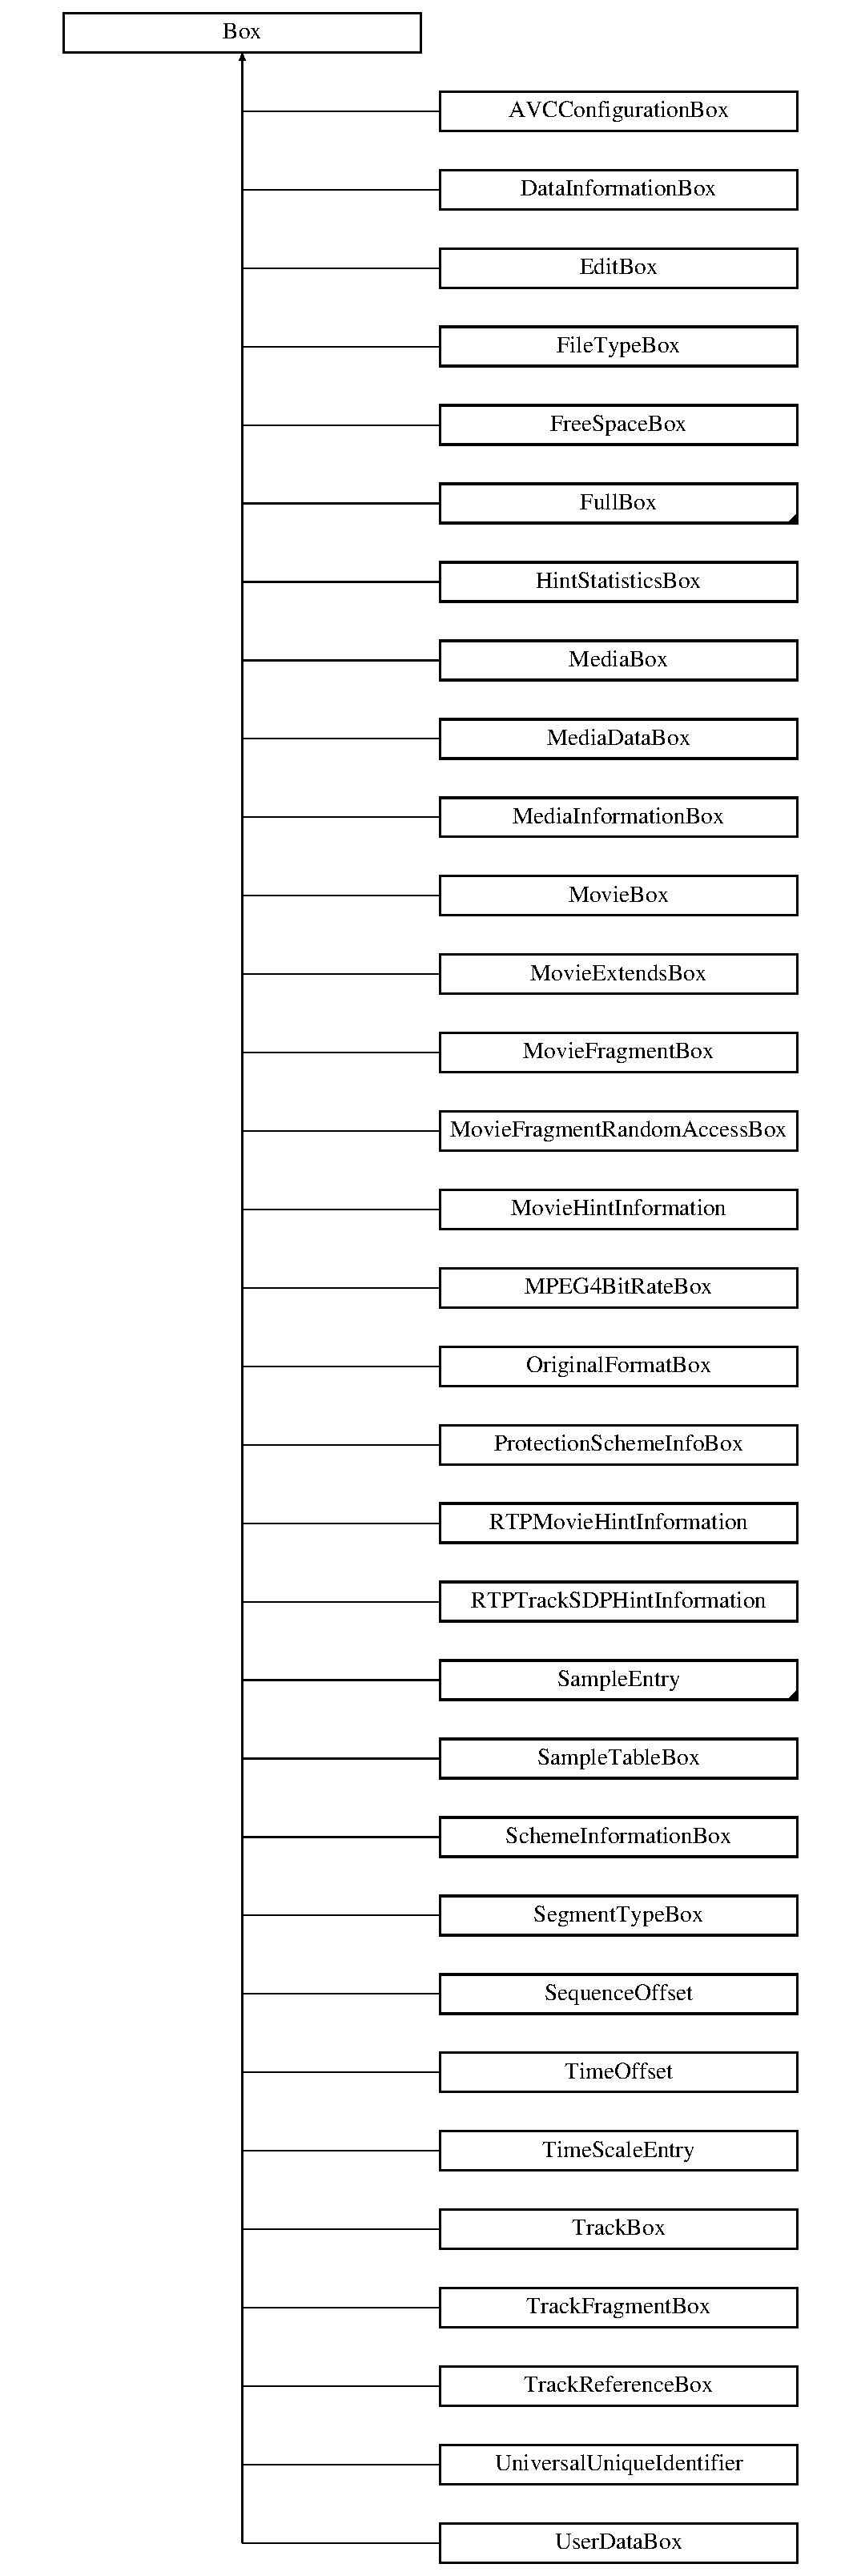
\includegraphics[height=12.000000cm]{class_box}
\end{center}
\end{figure}
\subsection*{Public Member Functions}
\begin{DoxyCompactItemize}
\item 
\hyperlink{class_box_a0cce9940febf67fa2e7af70c1884bc0f}{Box} (const unsigned int \&s, const Q\-String \&t, const unsigned long \&off)
\begin{DoxyCompactList}\small\item\em \hyperlink{class_box}{Box} constructor. \end{DoxyCompactList}\item 
virtual Q\-String \hyperlink{class_box_ab349afe9881614148ca93db089ae3723}{get\-Type} ()
\begin{DoxyCompactList}\small\item\em get\-Type \end{DoxyCompactList}\item 
virtual unsigned int \hyperlink{class_box_ae7997ebd366dd92a4f0604bae393ea77}{get\-Size} ()
\begin{DoxyCompactList}\small\item\em get\-Size \end{DoxyCompactList}\item 
virtual unsigned long int \hyperlink{class_box_a3aa52ebe50e92cffe331215c829f0328}{get\-Offset} () const 
\begin{DoxyCompactList}\small\item\em get\-Offset \end{DoxyCompactList}\item 
virtual bool \hyperlink{class_box_aa836717b34b2a26f84b6933d143da42b}{is\-Container} ()
\begin{DoxyCompactList}\small\item\em is\-Container \end{DoxyCompactList}\item 
virtual unsigned int \hyperlink{class_box_a2c9deb5e813bff43a2b2b62aafafe5b6}{get\-Container\-Offset} ()
\begin{DoxyCompactList}\small\item\em get\-Containet\-Offset \end{DoxyCompactList}\item 
virtual Q\-String \hyperlink{class_box_aa7c1e41e425cce53e0bd532cfafbb67d}{get\-Full\-Name} ()
\begin{DoxyCompactList}\small\item\em get\-Full\-Name \end{DoxyCompactList}\item 
virtual Q\-Standard\-Item\-Model $\ast$ \hyperlink{class_box_a5c7911f3c88eec77383c0a464979807d}{get\-Model} ()
\begin{DoxyCompactList}\small\item\em get\-Model Constructs and return Q\-Standard\-Item\-Model object that is appropriate for graphical representation (for elements like Q\-Tree\-View, Q\-Table\-View etc.). Returned model contains names of the box attributes and their value. Each pair it's in its own row. Name of the attribute is in column 0, value -\/ column 1. \end{DoxyCompactList}\end{DoxyCompactItemize}
\subsection*{Protected Attributes}
\begin{DoxyCompactItemize}
\item 
\hypertarget{class_box_a0c055cb66d94b40d80e8a18d3d52d230}{unsigned int \hyperlink{class_box_a0c055cb66d94b40d80e8a18d3d52d230}{size}}\label{class_box_a0c055cb66d94b40d80e8a18d3d52d230}

\begin{DoxyCompactList}\small\item\em size size of the box \end{DoxyCompactList}\item 
\hypertarget{class_box_a7222d6793ebff6bd17192a5c5740a78b}{Q\-String \hyperlink{class_box_a7222d6793ebff6bd17192a5c5740a78b}{type}}\label{class_box_a7222d6793ebff6bd17192a5c5740a78b}

\begin{DoxyCompactList}\small\item\em type type of the box \end{DoxyCompactList}\item 
\hypertarget{class_box_a02478afe7796308689a7929a5d17cd3d}{unsigned long int \hyperlink{class_box_a02478afe7796308689a7929a5d17cd3d}{offset}}\label{class_box_a02478afe7796308689a7929a5d17cd3d}

\begin{DoxyCompactList}\small\item\em offset byte offset of the box location \end{DoxyCompactList}\end{DoxyCompactItemize}


\subsection{Detailed Description}
The \hyperlink{class_box}{Box} class is representation of M\-P4 box. It contains parameters that all the classes should have. 

\begin{DoxySeeAlso}{See Also}
I\-S\-O/\-I\-E\-C 14496-\/12 Information technology – Coding of audio-\/visual objects – Part 12\-: I\-S\-O base media file format 
\end{DoxySeeAlso}


\subsection{Constructor \& Destructor Documentation}
\hypertarget{class_box_a0cce9940febf67fa2e7af70c1884bc0f}{\index{Box@{Box}!Box@{Box}}
\index{Box@{Box}!Box@{Box}}
\subsubsection[{Box}]{\setlength{\rightskip}{0pt plus 5cm}Box\-::\-Box (
\begin{DoxyParamCaption}
\item[{const unsigned int \&}]{s, }
\item[{const Q\-String \&}]{t, }
\item[{const unsigned long \&}]{off}
\end{DoxyParamCaption}
)}}\label{class_box_a0cce9940febf67fa2e7af70c1884bc0f}


\hyperlink{class_box}{Box} constructor. 


\begin{DoxyParams}{Parameters}
{\em s} & size of box in bytes \\
\hline
{\em t} & type of box (created from reading bytes in A\-S\-C\-I\-I code) \\
\hline
{\em off} & offset of box in bytes \\
\hline
\end{DoxyParams}


\subsection{Member Function Documentation}
\hypertarget{class_box_a2c9deb5e813bff43a2b2b62aafafe5b6}{\index{Box@{Box}!get\-Container\-Offset@{get\-Container\-Offset}}
\index{get\-Container\-Offset@{get\-Container\-Offset}!Box@{Box}}
\subsubsection[{get\-Container\-Offset}]{\setlength{\rightskip}{0pt plus 5cm}virtual unsigned int Box\-::get\-Container\-Offset (
\begin{DoxyParamCaption}
{}
\end{DoxyParamCaption}
)\hspace{0.3cm}{\ttfamily [inline]}, {\ttfamily [virtual]}}}\label{class_box_a2c9deb5e813bff43a2b2b62aafafe5b6}


get\-Containet\-Offset 

\begin{DoxyReturn}{Returns}
offset of child boxes in the box (in bytes) 
\end{DoxyReturn}


Reimplemented in \hyperlink{class_meta_box_a991bcf6b91fbe8f58b37118ccb2f44ca}{Meta\-Box}, \hyperlink{class_data_reference_box_a509baa8527d8fc5ff1d61d4e2508172f}{Data\-Reference\-Box}, \hyperlink{class_a_v_c_sample_entry_ab65d3ccefc8bcf0a0157d66189ecf8d8}{A\-V\-C\-Sample\-Entry}, \hyperlink{class_e_s_d_box_a17698371f055f5deec6e9819c9b302cd}{E\-S\-D\-Box}, \hyperlink{class_m_p4_audio_sample_entry_a81c5345f7b14c1fc8fe089dae5fd5793}{M\-P4\-Audio\-Sample\-Entry}, \hyperlink{class_m_p4_visual_sample_entry_a5ef15604b8bd6d3626dcbef1698346a9}{M\-P4\-Visual\-Sample\-Entry}, and \hyperlink{class_sample_description_box_af2fa7d915484805e19abf46f40e906f6}{Sample\-Description\-Box}.

\hypertarget{class_box_aa7c1e41e425cce53e0bd532cfafbb67d}{\index{Box@{Box}!get\-Full\-Name@{get\-Full\-Name}}
\index{get\-Full\-Name@{get\-Full\-Name}!Box@{Box}}
\subsubsection[{get\-Full\-Name}]{\setlength{\rightskip}{0pt plus 5cm}virtual Q\-String Box\-::get\-Full\-Name (
\begin{DoxyParamCaption}
{}
\end{DoxyParamCaption}
)\hspace{0.3cm}{\ttfamily [inline]}, {\ttfamily [virtual]}}}\label{class_box_aa7c1e41e425cce53e0bd532cfafbb67d}


get\-Full\-Name 

\begin{DoxyReturn}{Returns}
full\-Name of the box, e.\-g. \char`\"{}\-Media Data Box\char`\"{} 
\end{DoxyReturn}


Reimplemented in \hyperlink{class_universal_unique_identifier_aa2c40da68671ab3f272dcb8514921324}{Universal\-Unique\-Identifier}, \hyperlink{class_producer_reference_time_box_a989eb0b8ec1d3edc57b251e815cc246c}{Producer\-Reference\-Time\-Box}, \hyperlink{class_subsegment_index_box_ae476be69002235154639a5fe938eff60}{Subsegment\-Index\-Box}, \hyperlink{class_segment_index_box_a7e3ded610e2f9811909f2152071b7eb8}{Segment\-Index\-Box}, \hyperlink{class_level_assignment_box_a9b2449445de5d18f29915acce604d858}{Level\-Assignment\-Box}, \hyperlink{class_sample_auxiliary_information_offsets_box_a40dda3a60fe8424a9f31b964909b6fa5}{Sample\-Auxiliary\-Information\-Offsets\-Box}, \hyperlink{class_sample_auxiliary_information_sizes_box_af7c35b3682bb2ab65a0bf5b9ef58dd3e}{Sample\-Auxiliary\-Information\-Sizes\-Box}, \hyperlink{class_hint_statistics_box_acec0896d250145c53576fb9f079136ca}{Hint\-Statistics\-Box}, \hyperlink{class_r_t_p_track_s_d_p_hint_information_a4603595aa6393c8c9291e43d869c0313}{R\-T\-P\-Track\-S\-D\-P\-Hint\-Information}, \hyperlink{class_r_t_p_movie_hint_information_a392a45bf07f14c417c4acf3dde6b90d2}{R\-T\-P\-Movie\-Hint\-Information}, \hyperlink{class_movie_hint_information_ab85d823e7fd70195e0f066cd305dce1c}{Movie\-Hint\-Information}, \hyperlink{class_s_r_t_p_process_box_ae1f412cb4d3fe567a42226acd6b13542}{S\-R\-T\-P\-Process\-Box}, \hyperlink{class_sequence_offset_af94648de33aecf8edf6eb0d73565c991}{Sequence\-Offset}, \hyperlink{class_time_offset_a37cfed2c1ed2bb2cc6905c90e064cadb}{Time\-Offset}, \hyperlink{class_time_scale_entry_a0a6cd5076e6fd5a2ef2250985a602fd2}{Time\-Scale\-Entry}, \hyperlink{class_scheme_information_box_ac23d413584b8c7efe0693f42e8b05bcb}{Scheme\-Information\-Box}, \hyperlink{class_scheme_type_box_a0a66d06868e206070ba44ef2324e4e31}{Scheme\-Type\-Box}, \hyperlink{class_i_p_m_p_control_box_a5e9c6d323b59faa8d2d43ee2e24a4b33}{I\-P\-M\-P\-Control\-Box}, \hyperlink{class_i_p_m_p_info_box_aef8ac41ff48a6fa3ce83f81dbdd369a1}{I\-P\-M\-P\-Info\-Box}, \hyperlink{class_original_format_box_af113c3ee7fa52db04b3bb3c58aa09724}{Original\-Format\-Box}, \hyperlink{class_protection_scheme_info_box_a322ef8cac44eae717e95c395d80b9afe}{Protection\-Scheme\-Info\-Box}, \hyperlink{class_item_info_box_acc8b801d684beee63b12ea00aa84b1d4}{Item\-Info\-Box}, \hyperlink{class_item_info_entry_a7d744fa6aeb0ee948a898bb7b629a384}{Item\-Info\-Entry}, \hyperlink{class_item_protection_box_a282908379f31aeaacb0eac073050b132}{Item\-Protection\-Box}, \hyperlink{class_primary_item_box_a77154a0294bff85067fc8c6cddecb8f1}{Primary\-Item\-Box}, \hyperlink{class_item_location_box_a88ae4bd69cdcc39a4f54b894631c12fe}{Item\-Location\-Box}, \hyperlink{class_binary_x_m_l_box_a03f9dd3cec50f79bde9f6e861826badd}{Binary\-X\-M\-L\-Box}, \hyperlink{class_x_m_l_box_a430688e22c69256bfc823b979a5060c9}{X\-M\-L\-Box}, \hyperlink{class_meta_box_a2d7a7dced50efa9193cdb68a56a59e78}{Meta\-Box}, \hyperlink{class_progressive_download_info_box_a31f8b06687aff8fed0fc103c94636a7c}{Progressive\-Download\-Info\-Box}, \hyperlink{class_sub_sample_information_box_a8220480e149473cb07bd86e6dae71701}{Sub\-Sample\-Information\-Box}, \hyperlink{class_sample_scale_box_a10a781e0e86c780b2852359f5088bd9d}{Sample\-Scale\-Box}, \hyperlink{class_sample_group_description_box_a987897d30768742d06d40a4148c7c2ea}{Sample\-Group\-Description\-Box}, \hyperlink{class_sample_to_group_box_aa1cabba0625ae5ac6c32b63846e72957}{Sample\-To\-Group\-Box}, \hyperlink{class_sample_dependency_type_box_a2a8819e3085a47d092ddda32be36dbcd}{Sample\-Dependency\-Type\-Box}, \hyperlink{class_movie_fragment_random_access_offset_box_af4d75bd89f37a3e2de59d4e327924dff}{Movie\-Fragment\-Random\-Access\-Offset\-Box}, \hyperlink{class_movie_fragment_random_access_box_a6f57f73eaa945a9af8f5c512f5fd80da}{Movie\-Fragment\-Random\-Access\-Box}, \hyperlink{class_movie_fragment_header_box_a2a175cae00c09667bb8553e8e4ab7b16}{Movie\-Fragment\-Header\-Box}, \hyperlink{class_movie_fragment_box_a496f11dd218973b9eabc0d033cf489f5}{Movie\-Fragment\-Box}, \hyperlink{class_movie_extends_header_box_a04b51a9cf075645ba21dcaaa619407c9}{Movie\-Extends\-Header\-Box}, \hyperlink{class_movie_extends_box_ae61f578cd6f7e0e8f3eb1de0c1ae2c50}{Movie\-Extends\-Box}, \hyperlink{class_copy_right_box_a5aba245c42efd1c1c587a9a7ef1fc35c}{Copy\-Right\-Box}, \hyperlink{class_user_data_box_aa95cfad6fd0558e31894e76ed1bf8a20}{User\-Data\-Box}, \hyperlink{class_edit_list_box_a305003416ec092738d06298aaffbb47d}{Edit\-List\-Box}, \hyperlink{class_edit_box_a13ccdc9edfcb00039f5785bf1d33b30e}{Edit\-Box}, \hyperlink{class_free_space_box_a28d0e0e3e5111d4a741d03eeab1b40ea}{Free\-Space\-Box}, \hyperlink{class_data_reference_box_ac023a9fd6a4177dbe16569d3ced7fd1e}{Data\-Reference\-Box}, \hyperlink{class_data_entry_url_box_a33db27552c8aa8867b565b33fa3b43d5}{Data\-Entry\-Url\-Box}, \hyperlink{class_data_entry_urn_box_a85ff1a497b398ec76cdc74f28754927a}{Data\-Entry\-Urn\-Box}, \hyperlink{class_data_information_box_afb82c4d6fcfbdff60fd172a7d1e5800c}{Data\-Information\-Box}, \hyperlink{class_null_media_header_box_a1d934fede8322ee1eb4b5da2be999411}{Null\-Media\-Header\-Box}, \hyperlink{class_hint_media_header_box_aacaa05edc0b37296c6b0cad9b216babe}{Hint\-Media\-Header\-Box}, \hyperlink{class_sound_media_header_box_a942002b38261d7b015d9309ca02ccab6}{Sound\-Media\-Header\-Box}, \hyperlink{class_video_media_header_box_a6a6b15f956a608c18112b1b2b2317528}{Video\-Media\-Header\-Box}, \hyperlink{class_media_information_box_afa6c5040aa7d1533543100c0fbbc0e9d}{Media\-Information\-Box}, \hyperlink{class_movie_header_box_a90549b1eef690572412b138e3743e6c4}{Movie\-Header\-Box}, \hyperlink{class_m_p_e_g4_bit_rate_box_a5ee8e5653c4d5683e85c6b9f5b6746a1}{M\-P\-E\-G4\-Bit\-Rate\-Box}, \hyperlink{class_movie_box_a68e2952ae634633bbccaf61c749fa33f}{Movie\-Box}, \hyperlink{class_padding_bits_box_ab355f0ebfa4a84ef4a2737bc9c264004}{Padding\-Bits\-Box}, \hyperlink{class_degradation_priority_box_a97f91434e74e47bc9e10ff9a21dd3023}{Degradation\-Priority\-Box}, \hyperlink{class_a_v_c_configuration_box_a2cd37cfa63d1fa4130c6cd853a371e6f}{A\-V\-C\-Configuration\-Box}, \hyperlink{class_media_header_box_afa8deebe50a9958932c543a79e3c198c}{Media\-Header\-Box}, \hyperlink{class_shadow_sync_sample_box_ab6644ef80649f21ac098f0d78904e9df}{Shadow\-Sync\-Sample\-Box}, \hyperlink{class_handler_box_a77b90ca0801113aed5f6272035da0a04}{Handler\-Box}, \hyperlink{class_sync_sample_box_a9d3ab6e8730ca0cca633b7920e131413}{Sync\-Sample\-Box}, \hyperlink{class_media_data_box_a76ca0bfdfb66583db91784dd4d8e8ccb}{Media\-Data\-Box}, \hyperlink{class_a_v_c_sample_entry_a672f849ea0bd16cb832d1592ff8ae827}{A\-V\-C\-Sample\-Entry}, \hyperlink{class_track_fragment_base_media_decode_time_box_acf81a553080878b3066b24fc00b14f9e}{Track\-Fragment\-Base\-Media\-Decode\-Time\-Box}, \hyperlink{class_chunk_large_offset_box_acdadc159668e5e6ab286dbb840877f31}{Chunk\-Large\-Offset\-Box}, \hyperlink{class_media_box_a1fc835d61029b900e874039e2d29216e}{Media\-Box}, \hyperlink{class_e_s_d_box_a9e610dce6e72228e08fcbdfca0177c85}{E\-S\-D\-Box}, \hyperlink{class_track_fragment_random_access_box_afeb1c2b67373428008a209cf01f6df10}{Track\-Fragment\-Random\-Access\-Box}, \hyperlink{class_segment_type_box_aba34f8492af563e14e9f904eab862c62}{Segment\-Type\-Box}, \hyperlink{class_chunk_offset_box_a1c26ce6ada45f85c65761ed27f382848}{Chunk\-Offset\-Box}, \hyperlink{class_object_descriptor_box_ae01792b840bd4547ecc0aba4ee665998}{Object\-Descriptor\-Box}, \hyperlink{class_track_run_box_a26fb4feae53dac2aa48caaa39ccceb81}{Track\-Run\-Box}, \hyperlink{class_file_type_box_a680e45fdfe39b2e23ff46fc9f32153eb}{File\-Type\-Box}, \hyperlink{class_sample_to_chunk_box_a298e53e6d563e66b7b910f99caeac0c3}{Sample\-To\-Chunk\-Box}, \hyperlink{class_mpeg_sample_entry_ac07fbe3d0f06f9360acd2e60eb839928}{Mpeg\-Sample\-Entry}, \hyperlink{class_track_fragment_header_box_a6868fba2faed6053702b3c70751195e2}{Track\-Fragment\-Header\-Box}, \hyperlink{class_m_p4_audio_sample_entry_a81d787d905a0ee6fe1158daf8cddb64d}{M\-P4\-Audio\-Sample\-Entry}, \hyperlink{class_full_box_a0701464d8e7386653f025833308f76ee}{Full\-Box}, \hyperlink{class_compact_sample_size_box_a10c8ab4b452dd5c2d58e2c744ffac884}{Compact\-Sample\-Size\-Box}, \hyperlink{class_m_p4_visual_sample_entry_a82117470bd8bbda71839fff2b9a069c6}{M\-P4\-Visual\-Sample\-Entry}, \hyperlink{class_sample_size_box_a3cdb87618bba15d0c9e8cea9dde19ee5}{Sample\-Size\-Box}, \hyperlink{class_track_fragment_box_a1ab269642f375777c20b9ab52fbc72f7}{Track\-Fragment\-Box}, \hyperlink{class_audio_sample_entry_a928ab5498c0a8679ed624f9089dc5825}{Audio\-Sample\-Entry}, \hyperlink{class_track_extends_box_acaa1a49911d86e5ca02ce2038398ff5d}{Track\-Extends\-Box}, \hyperlink{class_sample_description_box_a47754fb62da6522d13ff58de1ede0f09}{Sample\-Description\-Box}, \hyperlink{class_visual_sample_entry_a8c48b121f4b5bb48d33bc9988a5dd856}{Visual\-Sample\-Entry}, \hyperlink{class_track_reference_box_ae140565faf9eb4e95fd8ab3de418c308}{Track\-Reference\-Box}, \hyperlink{class_composition_offset_box_a6ed0d84212f70f61a021b39e1114c0fb}{Composition\-Offset\-Box}, \hyperlink{class_track_header_box_a7bc710a767026e2128ae46a1d3302778}{Track\-Header\-Box}, \hyperlink{class_time_to_sample_box_a44c8086a9f61fb72f9549e8f997be7b9}{Time\-To\-Sample\-Box}, \hyperlink{class_hint_sample_entry_ac747c305de54a619efe66d5d8e0ec61a}{Hint\-Sample\-Entry}, \hyperlink{class_sample_table_box_acdaf2b1d02df4da6fee980f328d24dbb}{Sample\-Table\-Box}, \hyperlink{class_sample_entry_acbc7081715759b868797ad71b469a63e}{Sample\-Entry}, and \hyperlink{class_track_box_a2d45d42edb82a5445d54e184894aa730}{Track\-Box}.

\hypertarget{class_box_a5c7911f3c88eec77383c0a464979807d}{\index{Box@{Box}!get\-Model@{get\-Model}}
\index{get\-Model@{get\-Model}!Box@{Box}}
\subsubsection[{get\-Model}]{\setlength{\rightskip}{0pt plus 5cm}virtual Q\-Standard\-Item\-Model$\ast$ Box\-::get\-Model (
\begin{DoxyParamCaption}
{}
\end{DoxyParamCaption}
)\hspace{0.3cm}{\ttfamily [inline]}, {\ttfamily [virtual]}}}\label{class_box_a5c7911f3c88eec77383c0a464979807d}


get\-Model Constructs and return Q\-Standard\-Item\-Model object that is appropriate for graphical representation (for elements like Q\-Tree\-View, Q\-Table\-View etc.). Returned model contains names of the box attributes and their value. Each pair it's in its own row. Name of the attribute is in column 0, value -\/ column 1. 

\begin{DoxyReturn}{Returns}
model of \hyperlink{class_box}{Box} attributes 
\end{DoxyReturn}


Reimplemented in \hyperlink{class_segment_index_box_afc289658b786949624da7dc920ebd5e6}{Segment\-Index\-Box}, \hyperlink{class_movie_fragment_header_box_a768488b5d695c2ac834a041165a9be82}{Movie\-Fragment\-Header\-Box}, \hyperlink{class_movie_extends_header_box_adaeb21e662a49f852651f706af1b683a}{Movie\-Extends\-Header\-Box}, \hyperlink{class_edit_list_box_ab9a8848b0789b08e700447c3a279fcb4}{Edit\-List\-Box}, \hyperlink{class_data_reference_box_af73f1f378a20d2f705327cc815dc7396}{Data\-Reference\-Box}, \hyperlink{class_data_entry_url_box_a37fd12df4e0074f0bc2c8cc9cd3f7e5f}{Data\-Entry\-Url\-Box}, \hyperlink{class_sound_media_header_box_acc53b76481ed9c6e544b27c416f756e5}{Sound\-Media\-Header\-Box}, \hyperlink{class_video_media_header_box_aae14c3d53a5795039e3c5ccebc91d501}{Video\-Media\-Header\-Box}, \hyperlink{class_movie_header_box_a84bc9141e1de6ad9de73c00c9d861c7a}{Movie\-Header\-Box}, \hyperlink{class_m_p_e_g4_bit_rate_box_aee967785d4fb16f784b5b6dffcd850a8}{M\-P\-E\-G4\-Bit\-Rate\-Box}, \hyperlink{class_movie_box_a48d5f8248231d692efb16c7fdab53b31}{Movie\-Box}, \hyperlink{class_a_v_c_configuration_box_a034f358eb5231b98effd3835f81f538a}{A\-V\-C\-Configuration\-Box}, \hyperlink{class_media_header_box_a1754199a092cd0a1f0952883b119f375}{Media\-Header\-Box}, \hyperlink{class_handler_box_a3d0550ec682df1ea81856082f431bc28}{Handler\-Box}, \hyperlink{class_sync_sample_box_afe48e1f32651b46329c3834e642b18f9}{Sync\-Sample\-Box}, \hyperlink{class_media_data_box_af92d93a0b4a5d2051188ea0f7d555978}{Media\-Data\-Box}, \hyperlink{class_track_fragment_base_media_decode_time_box_a6a0cf2982f9e9a8a8ba5adf6c18d6caf}{Track\-Fragment\-Base\-Media\-Decode\-Time\-Box}, \hyperlink{class_chunk_large_offset_box_a16b02676650f3c08360bad4ac35470aa}{Chunk\-Large\-Offset\-Box}, \hyperlink{class_media_box_a3e4eae22e99bddfbcaac8c2950c542a1}{Media\-Box}, \hyperlink{class_segment_type_box_a0b2997e05595074bc692d87e1c12a3e1}{Segment\-Type\-Box}, \hyperlink{class_chunk_offset_box_aa9dfe2b91c236fca8b311c34d1b0a053}{Chunk\-Offset\-Box}, \hyperlink{class_track_run_box_ab2cc42d77e882ea0be127059ebda2c4d}{Track\-Run\-Box}, \hyperlink{class_file_type_box_a0d7a5d446140b1d10c9ab36233e87550}{File\-Type\-Box}, \hyperlink{class_sample_to_chunk_box_a503e73d6fda55a6dcbbf4c2b035d6fb8}{Sample\-To\-Chunk\-Box}, \hyperlink{class_track_fragment_header_box_ae27a4cc65245d755a88ae0661f568189}{Track\-Fragment\-Header\-Box}, \hyperlink{class_sample_size_box_a4ca94df68b61aebbe2c3b46b18a8d5e5}{Sample\-Size\-Box}, \hyperlink{class_track_fragment_box_a0a177d42598a374f5d187a3f968aeb01}{Track\-Fragment\-Box}, \hyperlink{class_audio_sample_entry_a8666027778c6cf9438d4af902c1793ab}{Audio\-Sample\-Entry}, \hyperlink{class_track_extends_box_a17e3133ff264960cb23e2431131da088}{Track\-Extends\-Box}, \hyperlink{class_sample_description_box_ae00adf8e73a8480b7299a88d9d65d88a}{Sample\-Description\-Box}, \hyperlink{class_visual_sample_entry_a475b074b66ad025a76c66888c0e24f46}{Visual\-Sample\-Entry}, \hyperlink{class_composition_offset_box_aeeeab60183eae5c832e9e46a055ba4e3}{Composition\-Offset\-Box}, \hyperlink{class_track_header_box_a59393dc4fe8791f266666f8f64efc510}{Track\-Header\-Box}, \hyperlink{class_time_to_sample_box_a28661d2be357ba4eb02e98c5026b619d}{Time\-To\-Sample\-Box}, \hyperlink{class_sample_table_box_a59a54b04800609fe96e3fbeaeaedfd13}{Sample\-Table\-Box}, \hyperlink{class_sample_entry_a0babc6ec796f6bf05a5e3e59d635ca79}{Sample\-Entry}, and \hyperlink{class_track_box_ab1412b2b26163ad23191427e6e934b90}{Track\-Box}.

\hypertarget{class_box_a3aa52ebe50e92cffe331215c829f0328}{\index{Box@{Box}!get\-Offset@{get\-Offset}}
\index{get\-Offset@{get\-Offset}!Box@{Box}}
\subsubsection[{get\-Offset}]{\setlength{\rightskip}{0pt plus 5cm}virtual unsigned long int Box\-::get\-Offset (
\begin{DoxyParamCaption}
{}
\end{DoxyParamCaption}
) const\hspace{0.3cm}{\ttfamily [inline]}, {\ttfamily [virtual]}}}\label{class_box_a3aa52ebe50e92cffe331215c829f0328}


get\-Offset 

\begin{DoxyReturn}{Returns}
offset of the box in bytes 
\end{DoxyReturn}
\hypertarget{class_box_ae7997ebd366dd92a4f0604bae393ea77}{\index{Box@{Box}!get\-Size@{get\-Size}}
\index{get\-Size@{get\-Size}!Box@{Box}}
\subsubsection[{get\-Size}]{\setlength{\rightskip}{0pt plus 5cm}virtual unsigned int Box\-::get\-Size (
\begin{DoxyParamCaption}
{}
\end{DoxyParamCaption}
)\hspace{0.3cm}{\ttfamily [inline]}, {\ttfamily [virtual]}}}\label{class_box_ae7997ebd366dd92a4f0604bae393ea77}


get\-Size 

\begin{DoxyReturn}{Returns}
size in bytes 
\end{DoxyReturn}
\hypertarget{class_box_ab349afe9881614148ca93db089ae3723}{\index{Box@{Box}!get\-Type@{get\-Type}}
\index{get\-Type@{get\-Type}!Box@{Box}}
\subsubsection[{get\-Type}]{\setlength{\rightskip}{0pt plus 5cm}virtual Q\-String Box\-::get\-Type (
\begin{DoxyParamCaption}
{}
\end{DoxyParamCaption}
)\hspace{0.3cm}{\ttfamily [inline]}, {\ttfamily [virtual]}}}\label{class_box_ab349afe9881614148ca93db089ae3723}


get\-Type 

\begin{DoxyReturn}{Returns}
type of the box 
\end{DoxyReturn}
\hypertarget{class_box_aa836717b34b2a26f84b6933d143da42b}{\index{Box@{Box}!is\-Container@{is\-Container}}
\index{is\-Container@{is\-Container}!Box@{Box}}
\subsubsection[{is\-Container}]{\setlength{\rightskip}{0pt plus 5cm}virtual bool Box\-::is\-Container (
\begin{DoxyParamCaption}
{}
\end{DoxyParamCaption}
)\hspace{0.3cm}{\ttfamily [inline]}, {\ttfamily [virtual]}}}\label{class_box_aa836717b34b2a26f84b6933d143da42b}


is\-Container 

\begin{DoxyReturn}{Returns}
true when box contains other boxes, false otherwise 
\end{DoxyReturn}


Reimplemented in \hyperlink{class_protection_scheme_info_box_ad5b64db8fc90bcc8cdbfc747ca09e48e}{Protection\-Scheme\-Info\-Box}, \hyperlink{class_item_protection_box_a3d1db2ceacc95601edf25808f3bcf4c3}{Item\-Protection\-Box}, \hyperlink{class_meta_box_a51ccaec850de68efb454358b2cf37522}{Meta\-Box}, \hyperlink{class_movie_fragment_random_access_box_a98067d945d3946d0bb3b41057b7bb24f}{Movie\-Fragment\-Random\-Access\-Box}, \hyperlink{class_movie_fragment_box_a10e2f1d3c5dc5c87fcbd35f88601af55}{Movie\-Fragment\-Box}, \hyperlink{class_movie_extends_box_a8b970223c7bc6518dc09a86a2398dc97}{Movie\-Extends\-Box}, \hyperlink{class_edit_box_a839c13a43cc4250ffe9c9747a3318bb2}{Edit\-Box}, \hyperlink{class_free_space_box_a704a3d5d180b53f0ef928be4213f6705}{Free\-Space\-Box}, \hyperlink{class_data_reference_box_ad78cbb0eb0ba1f25aee966178e4f2f0e}{Data\-Reference\-Box}, \hyperlink{class_data_information_box_a4423b54d49079a301760361e42fd4dbf}{Data\-Information\-Box}, \hyperlink{class_media_information_box_a5228b61c1967efca5ab2a1212872765a}{Media\-Information\-Box}, \hyperlink{class_m_p_e_g4_bit_rate_box_aafb5c5fe09ef9afbfe91e3cc5ce0ff5d}{M\-P\-E\-G4\-Bit\-Rate\-Box}, \hyperlink{class_movie_box_af75bd55df36733f36e9c9c3bde448d93}{Movie\-Box}, \hyperlink{class_a_v_c_configuration_box_a626fddbe3ea41877e8a8e97335948339}{A\-V\-C\-Configuration\-Box}, \hyperlink{class_a_v_c_sample_entry_ae0627e8954e878a70c9a67e337fd5d26}{A\-V\-C\-Sample\-Entry}, \hyperlink{class_media_box_a425be0e4e5c7bd559cea7e313da94e2d}{Media\-Box}, \hyperlink{class_mpeg_sample_entry_a264a9e2915c1a17f5c7e4ff7f59dab47}{Mpeg\-Sample\-Entry}, \hyperlink{class_m_p4_audio_sample_entry_a17ffcfa7b17574ed19bd38ccab77f705}{M\-P4\-Audio\-Sample\-Entry}, \hyperlink{class_m_p4_visual_sample_entry_aa683a32a4491a554bfc03b0fe1197bfc}{M\-P4\-Visual\-Sample\-Entry}, \hyperlink{class_track_fragment_box_a49538cd7fe1c888203eab7cee5cfb08c}{Track\-Fragment\-Box}, \hyperlink{class_sample_description_box_a227a7ad2f2d282a14cdbbed065fecfa5}{Sample\-Description\-Box}, \hyperlink{class_visual_sample_entry_a212a8d19ecf3236a8951c0161a85a72d}{Visual\-Sample\-Entry}, \hyperlink{class_sample_table_box_ad104b1eb63f6ce7926bbc7cee83fd29f}{Sample\-Table\-Box}, and \hyperlink{class_track_box_a9e3d52a20872169fc6f29c09f1e2ce95}{Track\-Box}.



The documentation for this class was generated from the following files\-:\begin{DoxyCompactItemize}
\item 
Model/\-Boxes/box.\-h\item 
Model/\-Boxes/box.\-cpp\end{DoxyCompactItemize}

\hypertarget{class_box_factory}{\section{Box\-Factory Class Reference}
\label{class_box_factory}\index{Box\-Factory@{Box\-Factory}}
}


The \hyperlink{class_box_factory}{Box\-Factory} class is a factory that creates \hyperlink{class_box}{Box} objects.  




{\ttfamily \#include $<$boxfactory.\-h$>$}

\subsection*{Public Member Functions}
\begin{DoxyCompactItemize}
\item 
\hyperlink{class_box_factory_af74b7bc4a67273516501a9d4cdd866d9}{Box\-Factory} (\hyperlink{class_analyzer}{Analyzer} $\ast$an)
\begin{DoxyCompactList}\small\item\em \hyperlink{class_box_factory}{Box\-Factory}. \end{DoxyCompactList}\item 
std\-::shared\-\_\-ptr$<$ \hyperlink{class_box}{Box} $>$ \hyperlink{class_box_factory_ac40e8b259f58eea47c0302f3227cd3f2}{get\-Box} (const unsigned int \&size=0, Q\-String type=\char`\"{}\char`\"{}, unsigned long int off=0)
\begin{DoxyCompactList}\small\item\em get\-Box creates \hyperlink{class_box}{Box} according to the given parameters and adds extra parameters depending on type of the box. \end{DoxyCompactList}\end{DoxyCompactItemize}


\subsection{Detailed Description}
The \hyperlink{class_box_factory}{Box\-Factory} class is a factory that creates \hyperlink{class_box}{Box} objects. 

\subsection{Constructor \& Destructor Documentation}
\hypertarget{class_box_factory_af74b7bc4a67273516501a9d4cdd866d9}{\index{Box\-Factory@{Box\-Factory}!Box\-Factory@{Box\-Factory}}
\index{Box\-Factory@{Box\-Factory}!BoxFactory@{Box\-Factory}}
\subsubsection[{Box\-Factory}]{\setlength{\rightskip}{0pt plus 5cm}Box\-Factory\-::\-Box\-Factory (
\begin{DoxyParamCaption}
\item[{{\bf Analyzer} $\ast$}]{an}
\end{DoxyParamCaption}
)}}\label{class_box_factory_af74b7bc4a67273516501a9d4cdd866d9}


\hyperlink{class_box_factory}{Box\-Factory}. 


\begin{DoxyParams}{Parameters}
{\em an} & analyzer that enables reading extra parameters of the box. \\
\hline
\end{DoxyParams}


\subsection{Member Function Documentation}
\hypertarget{class_box_factory_ac40e8b259f58eea47c0302f3227cd3f2}{\index{Box\-Factory@{Box\-Factory}!get\-Box@{get\-Box}}
\index{get\-Box@{get\-Box}!BoxFactory@{Box\-Factory}}
\subsubsection[{get\-Box}]{\setlength{\rightskip}{0pt plus 5cm}std\-::shared\-\_\-ptr$<$ {\bf Box} $>$ Box\-Factory\-::get\-Box (
\begin{DoxyParamCaption}
\item[{const unsigned int \&}]{size = {\ttfamily 0}, }
\item[{Q\-String}]{type = {\ttfamily \char`\"{}\char`\"{}}, }
\item[{unsigned long int}]{off = {\ttfamily 0}}
\end{DoxyParamCaption}
)}}\label{class_box_factory_ac40e8b259f58eea47c0302f3227cd3f2}


get\-Box creates \hyperlink{class_box}{Box} according to the given parameters and adds extra parameters depending on type of the box. 


\begin{DoxyParams}{Parameters}
{\em size} & size of the box \\
\hline
{\em type} & type of the box \\
\hline
{\em byte} & offset of the box location \\
\hline
\end{DoxyParams}
\begin{DoxyReturn}{Returns}
\hyperlink{class_box}{Box} created according to the given and extra parametrs 
\end{DoxyReturn}


The documentation for this class was generated from the following files\-:\begin{DoxyCompactItemize}
\item 
Model/\-Boxes/boxfactory.\-h\item 
Model/\-Boxes/boxfactory.\-cpp\end{DoxyCompactItemize}

\hypertarget{class_chunk_large_offset_box}{\section{Chunk\-Large\-Offset\-Box Class Reference}
\label{class_chunk_large_offset_box}\index{Chunk\-Large\-Offset\-Box@{Chunk\-Large\-Offset\-Box}}
}


The \hyperlink{class_chunk_large_offset_box}{Chunk\-Large\-Offset\-Box} class represents 'co64' box.  




{\ttfamily \#include $<$sampletablebox.\-h$>$}

Inheritance diagram for Chunk\-Large\-Offset\-Box\-:\begin{figure}[H]
\begin{center}
\leavevmode
\includegraphics[height=3.000000cm]{class_chunk_large_offset_box}
\end{center}
\end{figure}
\subsection*{Public Member Functions}
\begin{DoxyCompactItemize}
\item 
\hypertarget{class_chunk_large_offset_box_ab5be759993cf2d794c6ecdc1829e45f4}{{\bfseries Chunk\-Large\-Offset\-Box} (const unsigned int \&s, const Q\-String \&t, const unsigned long int \&off, const unsigned int \&v, const Q\-List$<$ unsigned int $>$ \&f, const unsigned long int \&ec, const Q\-List$<$ unsigned long int $>$ \&co)}\label{class_chunk_large_offset_box_ab5be759993cf2d794c6ecdc1829e45f4}

\item 
virtual Q\-String \hyperlink{class_chunk_large_offset_box_acdadc159668e5e6ab286dbb840877f31}{get\-Full\-Name} ()
\begin{DoxyCompactList}\small\item\em get\-Full\-Name \end{DoxyCompactList}\item 
virtual Q\-Standard\-Item\-Model $\ast$ \hyperlink{class_chunk_large_offset_box_a16b02676650f3c08360bad4ac35470aa}{get\-Model} ()
\begin{DoxyCompactList}\small\item\em get\-Model Constructs and return Q\-Standard\-Item\-Model object that is appropriate for graphical representation (for elements like Q\-Tree\-View, Q\-Table\-View etc.). Returned model contains names of the box attributes and their value. Each pair it's in its own row. Name of the attribute is in column 0, value -\/ column 1. \end{DoxyCompactList}\end{DoxyCompactItemize}
\subsection*{Additional Inherited Members}


\subsection{Detailed Description}
The \hyperlink{class_chunk_large_offset_box}{Chunk\-Large\-Offset\-Box} class represents 'co64' box. 

\begin{DoxySeeAlso}{See Also}
I\-S\-O/\-I\-E\-C 14496-\/12 Information technology – Coding of audio-\/visual objects – Part 12\-: I\-S\-O base media file format 
\end{DoxySeeAlso}


\subsection{Member Function Documentation}
\hypertarget{class_chunk_large_offset_box_acdadc159668e5e6ab286dbb840877f31}{\index{Chunk\-Large\-Offset\-Box@{Chunk\-Large\-Offset\-Box}!get\-Full\-Name@{get\-Full\-Name}}
\index{get\-Full\-Name@{get\-Full\-Name}!ChunkLargeOffsetBox@{Chunk\-Large\-Offset\-Box}}
\subsubsection[{get\-Full\-Name}]{\setlength{\rightskip}{0pt plus 5cm}virtual Q\-String Chunk\-Large\-Offset\-Box\-::get\-Full\-Name (
\begin{DoxyParamCaption}
{}
\end{DoxyParamCaption}
)\hspace{0.3cm}{\ttfamily [inline]}, {\ttfamily [virtual]}}}\label{class_chunk_large_offset_box_acdadc159668e5e6ab286dbb840877f31}


get\-Full\-Name 

\begin{DoxyReturn}{Returns}
full\-Name of the box, e.\-g. \char`\"{}\-Media Data Box\char`\"{} 
\end{DoxyReturn}


Reimplemented from \hyperlink{class_full_box_a0701464d8e7386653f025833308f76ee}{Full\-Box}.

\hypertarget{class_chunk_large_offset_box_a16b02676650f3c08360bad4ac35470aa}{\index{Chunk\-Large\-Offset\-Box@{Chunk\-Large\-Offset\-Box}!get\-Model@{get\-Model}}
\index{get\-Model@{get\-Model}!ChunkLargeOffsetBox@{Chunk\-Large\-Offset\-Box}}
\subsubsection[{get\-Model}]{\setlength{\rightskip}{0pt plus 5cm}Q\-Standard\-Item\-Model $\ast$ Chunk\-Large\-Offset\-Box\-::get\-Model (
\begin{DoxyParamCaption}
{}
\end{DoxyParamCaption}
)\hspace{0.3cm}{\ttfamily [virtual]}}}\label{class_chunk_large_offset_box_a16b02676650f3c08360bad4ac35470aa}


get\-Model Constructs and return Q\-Standard\-Item\-Model object that is appropriate for graphical representation (for elements like Q\-Tree\-View, Q\-Table\-View etc.). Returned model contains names of the box attributes and their value. Each pair it's in its own row. Name of the attribute is in column 0, value -\/ column 1. 

\begin{DoxyReturn}{Returns}
model of \hyperlink{class_box}{Box} attributes 
\end{DoxyReturn}


Reimplemented from \hyperlink{class_box_a5c7911f3c88eec77383c0a464979807d}{Box}.



The documentation for this class was generated from the following files\-:\begin{DoxyCompactItemize}
\item 
Model/\-Boxes/sampletablebox.\-h\item 
Model/\-Boxes/sampletablebox.\-cpp\end{DoxyCompactItemize}

\hypertarget{class_chunk_offset_box}{\section{Chunk\-Offset\-Box Class Reference}
\label{class_chunk_offset_box}\index{Chunk\-Offset\-Box@{Chunk\-Offset\-Box}}
}


The \hyperlink{class_chunk_offset_box}{Chunk\-Offset\-Box} class represents 'stco' box.  




{\ttfamily \#include $<$sampletablebox.\-h$>$}

Inheritance diagram for Chunk\-Offset\-Box\-:\begin{figure}[H]
\begin{center}
\leavevmode
\includegraphics[height=3.000000cm]{class_chunk_offset_box}
\end{center}
\end{figure}
\subsection*{Public Member Functions}
\begin{DoxyCompactItemize}
\item 
\hypertarget{class_chunk_offset_box_a5a86166fb59bfa186c7a4094aacd4645}{{\bfseries Chunk\-Offset\-Box} (const unsigned long int \&s, const Q\-String \&t, const unsigned long int \&off, const unsigned int \&v, const Q\-List$<$ unsigned int $>$ \&f, const unsigned int \&ec, const Q\-List$<$ unsigned int $>$ \&co)}\label{class_chunk_offset_box_a5a86166fb59bfa186c7a4094aacd4645}

\item 
virtual Q\-String \hyperlink{class_chunk_offset_box_a1c26ce6ada45f85c65761ed27f382848}{get\-Full\-Name} ()
\begin{DoxyCompactList}\small\item\em get\-Full\-Name \end{DoxyCompactList}\item 
virtual Q\-Standard\-Item\-Model $\ast$ \hyperlink{class_chunk_offset_box_aa9dfe2b91c236fca8b311c34d1b0a053}{get\-Model} ()
\begin{DoxyCompactList}\small\item\em get\-Model Constructs and return Q\-Standard\-Item\-Model object that is appropriate for graphical representation (for elements like Q\-Tree\-View, Q\-Table\-View etc.). Returned model contains names of the box attributes and their value. Each pair it's in its own row. Name of the attribute is in column 0, value -\/ column 1. \end{DoxyCompactList}\end{DoxyCompactItemize}
\subsection*{Additional Inherited Members}


\subsection{Detailed Description}
The \hyperlink{class_chunk_offset_box}{Chunk\-Offset\-Box} class represents 'stco' box. 

\begin{DoxySeeAlso}{See Also}
I\-S\-O/\-I\-E\-C 14496-\/12 Information technology – Coding of audio-\/visual objects – Part 12\-: I\-S\-O base media file format 
\end{DoxySeeAlso}


\subsection{Member Function Documentation}
\hypertarget{class_chunk_offset_box_a1c26ce6ada45f85c65761ed27f382848}{\index{Chunk\-Offset\-Box@{Chunk\-Offset\-Box}!get\-Full\-Name@{get\-Full\-Name}}
\index{get\-Full\-Name@{get\-Full\-Name}!ChunkOffsetBox@{Chunk\-Offset\-Box}}
\subsubsection[{get\-Full\-Name}]{\setlength{\rightskip}{0pt plus 5cm}virtual Q\-String Chunk\-Offset\-Box\-::get\-Full\-Name (
\begin{DoxyParamCaption}
{}
\end{DoxyParamCaption}
)\hspace{0.3cm}{\ttfamily [inline]}, {\ttfamily [virtual]}}}\label{class_chunk_offset_box_a1c26ce6ada45f85c65761ed27f382848}


get\-Full\-Name 

\begin{DoxyReturn}{Returns}
full\-Name of the box, e.\-g. \char`\"{}\-Media Data Box\char`\"{} 
\end{DoxyReturn}


Reimplemented from \hyperlink{class_full_box_a0701464d8e7386653f025833308f76ee}{Full\-Box}.

\hypertarget{class_chunk_offset_box_aa9dfe2b91c236fca8b311c34d1b0a053}{\index{Chunk\-Offset\-Box@{Chunk\-Offset\-Box}!get\-Model@{get\-Model}}
\index{get\-Model@{get\-Model}!ChunkOffsetBox@{Chunk\-Offset\-Box}}
\subsubsection[{get\-Model}]{\setlength{\rightskip}{0pt plus 5cm}Q\-Standard\-Item\-Model $\ast$ Chunk\-Offset\-Box\-::get\-Model (
\begin{DoxyParamCaption}
{}
\end{DoxyParamCaption}
)\hspace{0.3cm}{\ttfamily [virtual]}}}\label{class_chunk_offset_box_aa9dfe2b91c236fca8b311c34d1b0a053}


get\-Model Constructs and return Q\-Standard\-Item\-Model object that is appropriate for graphical representation (for elements like Q\-Tree\-View, Q\-Table\-View etc.). Returned model contains names of the box attributes and their value. Each pair it's in its own row. Name of the attribute is in column 0, value -\/ column 1. 

\begin{DoxyReturn}{Returns}
model of \hyperlink{class_box}{Box} attributes 
\end{DoxyReturn}


Reimplemented from \hyperlink{class_box_a5c7911f3c88eec77383c0a464979807d}{Box}.



The documentation for this class was generated from the following files\-:\begin{DoxyCompactItemize}
\item 
Model/\-Boxes/sampletablebox.\-h\item 
Model/\-Boxes/sampletablebox.\-cpp\end{DoxyCompactItemize}

\hypertarget{class_compact_sample_size_box}{\section{Compact\-Sample\-Size\-Box Class Reference}
\label{class_compact_sample_size_box}\index{Compact\-Sample\-Size\-Box@{Compact\-Sample\-Size\-Box}}
}


The \hyperlink{class_compact_sample_size_box}{Compact\-Sample\-Size\-Box} class represents 'stz2' box.  




{\ttfamily \#include $<$sampletablebox.\-h$>$}

Inheritance diagram for Compact\-Sample\-Size\-Box\-:\begin{figure}[H]
\begin{center}
\leavevmode
\includegraphics[height=3.000000cm]{class_compact_sample_size_box}
\end{center}
\end{figure}
\subsection*{Public Member Functions}
\begin{DoxyCompactItemize}
\item 
\hypertarget{class_compact_sample_size_box_aadd7045acff4abdf1562c9de33dcfba0}{{\bfseries Compact\-Sample\-Size\-Box} (const unsigned int \&s, const Q\-String \&t, const unsigned long int \&off, const unsigned int \&v, const Q\-List$<$ unsigned int $>$ \&f)}\label{class_compact_sample_size_box_aadd7045acff4abdf1562c9de33dcfba0}

\item 
virtual Q\-String \hyperlink{class_compact_sample_size_box_a10c8ab4b452dd5c2d58e2c744ffac884}{get\-Full\-Name} ()
\begin{DoxyCompactList}\small\item\em get\-Full\-Name \end{DoxyCompactList}\end{DoxyCompactItemize}
\subsection*{Additional Inherited Members}


\subsection{Detailed Description}
The \hyperlink{class_compact_sample_size_box}{Compact\-Sample\-Size\-Box} class represents 'stz2' box. 

\begin{DoxySeeAlso}{See Also}
I\-S\-O/\-I\-E\-C 14496-\/12 Information technology – Coding of audio-\/visual objects – Part 12\-: I\-S\-O base media file format 
\end{DoxySeeAlso}


\subsection{Member Function Documentation}
\hypertarget{class_compact_sample_size_box_a10c8ab4b452dd5c2d58e2c744ffac884}{\index{Compact\-Sample\-Size\-Box@{Compact\-Sample\-Size\-Box}!get\-Full\-Name@{get\-Full\-Name}}
\index{get\-Full\-Name@{get\-Full\-Name}!CompactSampleSizeBox@{Compact\-Sample\-Size\-Box}}
\subsubsection[{get\-Full\-Name}]{\setlength{\rightskip}{0pt plus 5cm}virtual Q\-String Compact\-Sample\-Size\-Box\-::get\-Full\-Name (
\begin{DoxyParamCaption}
{}
\end{DoxyParamCaption}
)\hspace{0.3cm}{\ttfamily [inline]}, {\ttfamily [virtual]}}}\label{class_compact_sample_size_box_a10c8ab4b452dd5c2d58e2c744ffac884}


get\-Full\-Name 

\begin{DoxyReturn}{Returns}
full\-Name of the box, e.\-g. \char`\"{}\-Media Data Box\char`\"{} 
\end{DoxyReturn}


Reimplemented from \hyperlink{class_full_box_a0701464d8e7386653f025833308f76ee}{Full\-Box}.



The documentation for this class was generated from the following files\-:\begin{DoxyCompactItemize}
\item 
Model/\-Boxes/sampletablebox.\-h\item 
Model/\-Boxes/sampletablebox.\-cpp\end{DoxyCompactItemize}

\hypertarget{class_composition_offset_box}{\section{Composition\-Offset\-Box Class Reference}
\label{class_composition_offset_box}\index{Composition\-Offset\-Box@{Composition\-Offset\-Box}}
}


The \hyperlink{class_composition_offset_box}{Composition\-Offset\-Box} class represents 'ctts' box.  




{\ttfamily \#include $<$sampletablebox.\-h$>$}

Inheritance diagram for Composition\-Offset\-Box\-:\begin{figure}[H]
\begin{center}
\leavevmode
\includegraphics[height=3.000000cm]{class_composition_offset_box}
\end{center}
\end{figure}
\subsection*{Public Member Functions}
\begin{DoxyCompactItemize}
\item 
\hypertarget{class_composition_offset_box_a4c0b13fc3e5957cd288cf73a6b247b6a}{{\bfseries Composition\-Offset\-Box} (const unsigned long int \&s, const Q\-String \&t, const unsigned long int \&off, const unsigned int \&v, const Q\-List$<$ unsigned int $>$ \&f, unsigned int ec, Q\-List$<$ unsigned int $>$ sc, Q\-List$<$ unsigned int $>$ sd)}\label{class_composition_offset_box_a4c0b13fc3e5957cd288cf73a6b247b6a}

\item 
virtual Q\-String \hyperlink{class_composition_offset_box_a6ed0d84212f70f61a021b39e1114c0fb}{get\-Full\-Name} ()
\begin{DoxyCompactList}\small\item\em get\-Full\-Name \end{DoxyCompactList}\item 
virtual Q\-Standard\-Item\-Model $\ast$ \hyperlink{class_composition_offset_box_aeeeab60183eae5c832e9e46a055ba4e3}{get\-Model} ()
\begin{DoxyCompactList}\small\item\em get\-Model Constructs and return Q\-Standard\-Item\-Model object that is appropriate for graphical representation (for elements like Q\-Tree\-View, Q\-Table\-View etc.). Returned model contains names of the box attributes and their value. Each pair it's in its own row. Name of the attribute is in column 0, value -\/ column 1. \end{DoxyCompactList}\end{DoxyCompactItemize}
\subsection*{Additional Inherited Members}


\subsection{Detailed Description}
The \hyperlink{class_composition_offset_box}{Composition\-Offset\-Box} class represents 'ctts' box. 

\begin{DoxySeeAlso}{See Also}
I\-S\-O/\-I\-E\-C 14496-\/12 Information technology – Coding of audio-\/visual objects – Part 12\-: I\-S\-O base media file format 
\end{DoxySeeAlso}


\subsection{Member Function Documentation}
\hypertarget{class_composition_offset_box_a6ed0d84212f70f61a021b39e1114c0fb}{\index{Composition\-Offset\-Box@{Composition\-Offset\-Box}!get\-Full\-Name@{get\-Full\-Name}}
\index{get\-Full\-Name@{get\-Full\-Name}!CompositionOffsetBox@{Composition\-Offset\-Box}}
\subsubsection[{get\-Full\-Name}]{\setlength{\rightskip}{0pt plus 5cm}virtual Q\-String Composition\-Offset\-Box\-::get\-Full\-Name (
\begin{DoxyParamCaption}
{}
\end{DoxyParamCaption}
)\hspace{0.3cm}{\ttfamily [inline]}, {\ttfamily [virtual]}}}\label{class_composition_offset_box_a6ed0d84212f70f61a021b39e1114c0fb}


get\-Full\-Name 

\begin{DoxyReturn}{Returns}
full\-Name of the box, e.\-g. \char`\"{}\-Media Data Box\char`\"{} 
\end{DoxyReturn}


Reimplemented from \hyperlink{class_full_box_a0701464d8e7386653f025833308f76ee}{Full\-Box}.

\hypertarget{class_composition_offset_box_aeeeab60183eae5c832e9e46a055ba4e3}{\index{Composition\-Offset\-Box@{Composition\-Offset\-Box}!get\-Model@{get\-Model}}
\index{get\-Model@{get\-Model}!CompositionOffsetBox@{Composition\-Offset\-Box}}
\subsubsection[{get\-Model}]{\setlength{\rightskip}{0pt plus 5cm}Q\-Standard\-Item\-Model $\ast$ Composition\-Offset\-Box\-::get\-Model (
\begin{DoxyParamCaption}
{}
\end{DoxyParamCaption}
)\hspace{0.3cm}{\ttfamily [virtual]}}}\label{class_composition_offset_box_aeeeab60183eae5c832e9e46a055ba4e3}


get\-Model Constructs and return Q\-Standard\-Item\-Model object that is appropriate for graphical representation (for elements like Q\-Tree\-View, Q\-Table\-View etc.). Returned model contains names of the box attributes and their value. Each pair it's in its own row. Name of the attribute is in column 0, value -\/ column 1. 

\begin{DoxyReturn}{Returns}
model of \hyperlink{class_box}{Box} attributes 
\end{DoxyReturn}


Reimplemented from \hyperlink{class_box_a5c7911f3c88eec77383c0a464979807d}{Box}.



The documentation for this class was generated from the following files\-:\begin{DoxyCompactItemize}
\item 
Model/\-Boxes/sampletablebox.\-h\item 
Model/\-Boxes/sampletablebox.\-cpp\end{DoxyCompactItemize}

\hypertarget{class_controller}{\section{Controller Class Reference}
\label{class_controller}\index{Controller@{Controller}}
}


The \hyperlink{class_controller}{Controller} class The class defines methods that enable to control the application. It gets info about events generated by users by receiving signals and defines response to them.  




{\ttfamily \#include $<$controller.\-h$>$}

Inheritance diagram for Controller\-:\begin{figure}[H]
\begin{center}
\leavevmode
\includegraphics[height=2.000000cm]{class_controller}
\end{center}
\end{figure}
\subsection*{Public Member Functions}
\begin{DoxyCompactItemize}
\item 
\hyperlink{class_controller_a7925b6f339420ce2581a4c23c2f4a58c}{Controller} (\hyperlink{class_main_window}{Main\-Window} $\ast$mw)
\begin{DoxyCompactList}\small\item\em \hyperlink{class_controller}{Controller}. \end{DoxyCompactList}\end{DoxyCompactItemize}


\subsection{Detailed Description}
The \hyperlink{class_controller}{Controller} class The class defines methods that enable to control the application. It gets info about events generated by users by receiving signals and defines response to them. 

\subsection{Constructor \& Destructor Documentation}
\hypertarget{class_controller_a7925b6f339420ce2581a4c23c2f4a58c}{\index{Controller@{Controller}!Controller@{Controller}}
\index{Controller@{Controller}!Controller@{Controller}}
\subsubsection[{Controller}]{\setlength{\rightskip}{0pt plus 5cm}Controller\-::\-Controller (
\begin{DoxyParamCaption}
\item[{{\bf Main\-Window} $\ast$}]{mw}
\end{DoxyParamCaption}
)}}\label{class_controller_a7925b6f339420ce2581a4c23c2f4a58c}


\hyperlink{class_controller}{Controller}. 


\begin{DoxyParams}{Parameters}
{\em mw} & main window of the application \\
\hline
\end{DoxyParams}


The documentation for this class was generated from the following files\-:\begin{DoxyCompactItemize}
\item 
C\-O\-N\-T\-R\-O\-L\-L\-E\-R/controller.\-h\item 
C\-O\-N\-T\-R\-O\-L\-L\-E\-R/controller.\-cpp\end{DoxyCompactItemize}

\hypertarget{class_copy_right_box}{\section{Copy\-Right\-Box Class Reference}
\label{class_copy_right_box}\index{Copy\-Right\-Box@{Copy\-Right\-Box}}
}


The \hyperlink{class_copy_right_box}{Copy\-Right\-Box} class represents 'cprt' box.  




{\ttfamily \#include $<$box.\-h$>$}

Inheritance diagram for Copy\-Right\-Box\-:\begin{figure}[H]
\begin{center}
\leavevmode
\includegraphics[height=3.000000cm]{class_copy_right_box}
\end{center}
\end{figure}
\subsection*{Public Member Functions}
\begin{DoxyCompactItemize}
\item 
\hypertarget{class_copy_right_box_a130cfb7dee18f0d2b78e39d679ba3000}{{\bfseries Copy\-Right\-Box} (const unsigned int \&s, const Q\-String \&t, const unsigned long int \&off, const unsigned int \&v, const Q\-List$<$ unsigned int $>$ \&f)}\label{class_copy_right_box_a130cfb7dee18f0d2b78e39d679ba3000}

\item 
virtual Q\-String \hyperlink{class_copy_right_box_a5aba245c42efd1c1c587a9a7ef1fc35c}{get\-Full\-Name} ()
\begin{DoxyCompactList}\small\item\em get\-Full\-Name \end{DoxyCompactList}\end{DoxyCompactItemize}
\subsection*{Additional Inherited Members}


\subsection{Detailed Description}
The \hyperlink{class_copy_right_box}{Copy\-Right\-Box} class represents 'cprt' box. 

\begin{DoxySeeAlso}{See Also}
I\-S\-O/\-I\-E\-C 14496-\/12 Information technology – Coding of audio-\/visual objects – Part 12\-: I\-S\-O base media file format 
\end{DoxySeeAlso}


\subsection{Member Function Documentation}
\hypertarget{class_copy_right_box_a5aba245c42efd1c1c587a9a7ef1fc35c}{\index{Copy\-Right\-Box@{Copy\-Right\-Box}!get\-Full\-Name@{get\-Full\-Name}}
\index{get\-Full\-Name@{get\-Full\-Name}!CopyRightBox@{Copy\-Right\-Box}}
\subsubsection[{get\-Full\-Name}]{\setlength{\rightskip}{0pt plus 5cm}virtual Q\-String Copy\-Right\-Box\-::get\-Full\-Name (
\begin{DoxyParamCaption}
{}
\end{DoxyParamCaption}
)\hspace{0.3cm}{\ttfamily [inline]}, {\ttfamily [virtual]}}}\label{class_copy_right_box_a5aba245c42efd1c1c587a9a7ef1fc35c}


get\-Full\-Name 

\begin{DoxyReturn}{Returns}
full\-Name of the box, e.\-g. \char`\"{}\-Media Data Box\char`\"{} 
\end{DoxyReturn}


Reimplemented from \hyperlink{class_full_box_a0701464d8e7386653f025833308f76ee}{Full\-Box}.



The documentation for this class was generated from the following files\-:\begin{DoxyCompactItemize}
\item 
Model/\-Boxes/box.\-h\item 
Model/\-Boxes/box.\-cpp\end{DoxyCompactItemize}

\hypertarget{class_dash_creator}{\section{Dash\-Creator Class Reference}
\label{class_dash_creator}\index{Dash\-Creator@{Dash\-Creator}}
}


The \hyperlink{class_dash_creator}{Dash\-Creator} class provides several methods that enables writing mp4 dash file. The file may be streamed via internet according to M\-P\-E\-G-\/\-D\-A\-S\-H standard.  




{\ttfamily \#include $<$dashcreator.\-h$>$}

\subsection*{Public Member Functions}
\begin{DoxyCompactItemize}
\item 
\hypertarget{class_dash_creator_af4545342e3a1ab0aac61e1b0b6265370}{{\bfseries Dash\-Creator} (const Q\-String \&path, const Q\-String \&name, \hyperlink{class_tree_model}{Tree\-Model} $\ast$mod)}\label{class_dash_creator_af4545342e3a1ab0aac61e1b0b6265370}

\item 
\hypertarget{class_dash_creator_adb1268e79a32fe34c75bed9b04a1357e}{bool {\bfseries write\-File} (const unsigned int \&max\-Sample\-Num)}\label{class_dash_creator_adb1268e79a32fe34c75bed9b04a1357e}

\item 
\hypertarget{class_dash_creator_a324d4deedf4f0e06881aeef712e79917}{bool {\bfseries write\-Files} (const unsigned int \&max\-Sample\-Num)}\label{class_dash_creator_a324d4deedf4f0e06881aeef712e79917}

\end{DoxyCompactItemize}


\subsection{Detailed Description}
The \hyperlink{class_dash_creator}{Dash\-Creator} class provides several methods that enables writing mp4 dash file. The file may be streamed via internet according to M\-P\-E\-G-\/\-D\-A\-S\-H standard. 

The documentation for this class was generated from the following files\-:\begin{DoxyCompactItemize}
\item 
Model/\-Dash/dashcreator.\-h\item 
Model/\-Dash/dashcreator.\-cpp\end{DoxyCompactItemize}

\hypertarget{class_dash_section}{\section{Dash\-Section Class Reference}
\label{class_dash_section}\index{Dash\-Section@{Dash\-Section}}
}


The \hyperlink{class_dash_section}{Dash\-Section} class \hyperlink{class_dash_section}{Dash\-Section} contains and displays widgets that build view of dash section of the application.  




{\ttfamily \#include $<$dashsection.\-h$>$}

Inheritance diagram for Dash\-Section\-:\begin{figure}[H]
\begin{center}
\leavevmode
\includegraphics[height=2.000000cm]{class_dash_section}
\end{center}
\end{figure}
\subsection*{Signals}
\begin{DoxyCompactItemize}
\item 
void \hyperlink{class_dash_section_a1def7fe671027a0aa457ef3928c5c584}{dash\-Dir\-Sig} (const Q\-String \&dir)
\begin{DoxyCompactList}\small\item\em dash\-Dir\-Sig \end{DoxyCompactList}\item 
void \hyperlink{class_dash_section_aa5d208d28ce0ca70904b5a709d714958}{remove\-File\-Sig} (const int \&row)
\begin{DoxyCompactList}\small\item\em remove\-File\-Sig \end{DoxyCompactList}\item 
void \hyperlink{class_dash_section_af294c83b94ff52df6a21aa6c01d681b2}{dash\-Files\-Selected\-Signal} (const bool \&one\-File, const Q\-String \&url)
\begin{DoxyCompactList}\small\item\em dash\-Files\-Selected\-Signal \end{DoxyCompactList}\end{DoxyCompactItemize}
\subsection*{Public Member Functions}
\begin{DoxyCompactItemize}
\item 
\hyperlink{class_dash_section_a5dffdfc94fbff1f7373350b46943f0e1}{Dash\-Section} (Q\-Widget $\ast$parent=0)
\begin{DoxyCompactList}\small\item\em \hyperlink{class_dash_section}{Dash\-Section}. \end{DoxyCompactList}\item 
void \hyperlink{class_dash_section_abd3bb2f76089674e16a956ec3f6cd4d8}{set\-Dash\-File\-List} (Q\-Abstract\-Item\-Model $\ast$file\-Model, const bool \&disabled=false)
\begin{DoxyCompactList}\small\item\em set\-Dash\-File\-List \end{DoxyCompactList}\end{DoxyCompactItemize}


\subsection{Detailed Description}
The \hyperlink{class_dash_section}{Dash\-Section} class \hyperlink{class_dash_section}{Dash\-Section} contains and displays widgets that build view of dash section of the application. 

\subsection{Constructor \& Destructor Documentation}
\hypertarget{class_dash_section_a5dffdfc94fbff1f7373350b46943f0e1}{\index{Dash\-Section@{Dash\-Section}!Dash\-Section@{Dash\-Section}}
\index{Dash\-Section@{Dash\-Section}!DashSection@{Dash\-Section}}
\subsubsection[{Dash\-Section}]{\setlength{\rightskip}{0pt plus 5cm}Dash\-Section\-::\-Dash\-Section (
\begin{DoxyParamCaption}
\item[{Q\-Widget $\ast$}]{parent = {\ttfamily 0}}
\end{DoxyParamCaption}
)\hspace{0.3cm}{\ttfamily [explicit]}}}\label{class_dash_section_a5dffdfc94fbff1f7373350b46943f0e1}


\hyperlink{class_dash_section}{Dash\-Section}. 

Public.


\begin{DoxyParams}{Parameters}
{\em model} & tree model of boxes \\
\hline
{\em parent} & Creates dash section. It contains of filenames listview, buttons (selecting directory of files, removing file from list and preparing selected files to dash streaming) and textline of U\-R\-L address. \\
\hline
\end{DoxyParams}


\subsection{Member Function Documentation}
\hypertarget{class_dash_section_a1def7fe671027a0aa457ef3928c5c584}{\index{Dash\-Section@{Dash\-Section}!dash\-Dir\-Sig@{dash\-Dir\-Sig}}
\index{dash\-Dir\-Sig@{dash\-Dir\-Sig}!DashSection@{Dash\-Section}}
\subsubsection[{dash\-Dir\-Sig}]{\setlength{\rightskip}{0pt plus 5cm}void Dash\-Section\-::dash\-Dir\-Sig (
\begin{DoxyParamCaption}
\item[{const Q\-String \&}]{dir}
\end{DoxyParamCaption}
)\hspace{0.3cm}{\ttfamily [signal]}}}\label{class_dash_section_a1def7fe671027a0aa457ef3928c5c584}


dash\-Dir\-Sig 


\begin{DoxyParams}{Parameters}
{\em dir} & selected directory \\
\hline
\end{DoxyParams}
\hypertarget{class_dash_section_af294c83b94ff52df6a21aa6c01d681b2}{\index{Dash\-Section@{Dash\-Section}!dash\-Files\-Selected\-Signal@{dash\-Files\-Selected\-Signal}}
\index{dash\-Files\-Selected\-Signal@{dash\-Files\-Selected\-Signal}!DashSection@{Dash\-Section}}
\subsubsection[{dash\-Files\-Selected\-Signal}]{\setlength{\rightskip}{0pt plus 5cm}void Dash\-Section\-::dash\-Files\-Selected\-Signal (
\begin{DoxyParamCaption}
\item[{const bool \&}]{one\-File, }
\item[{const Q\-String \&}]{url}
\end{DoxyParamCaption}
)\hspace{0.3cm}{\ttfamily [signal]}}}\label{class_dash_section_af294c83b94ff52df6a21aa6c01d681b2}


dash\-Files\-Selected\-Signal 


\begin{DoxyParams}{Parameters}
{\em one\-File} & indicates whether all segments of each presentation should be gathered in one file \\
\hline
{\em url} & U\-R\-L address where generated files will be available. It is inserted into \hyperlink{class_m_p_d}{M\-P\-D} file. \\
\hline
\end{DoxyParams}
\hypertarget{class_dash_section_aa5d208d28ce0ca70904b5a709d714958}{\index{Dash\-Section@{Dash\-Section}!remove\-File\-Sig@{remove\-File\-Sig}}
\index{remove\-File\-Sig@{remove\-File\-Sig}!DashSection@{Dash\-Section}}
\subsubsection[{remove\-File\-Sig}]{\setlength{\rightskip}{0pt plus 5cm}void Dash\-Section\-::remove\-File\-Sig (
\begin{DoxyParamCaption}
\item[{const int \&}]{row}
\end{DoxyParamCaption}
)\hspace{0.3cm}{\ttfamily [signal]}}}\label{class_dash_section_aa5d208d28ce0ca70904b5a709d714958}


remove\-File\-Sig 


\begin{DoxyParams}{Parameters}
{\em row} & row id of the filename record that shall be removed from the list \\
\hline
\end{DoxyParams}
\hypertarget{class_dash_section_abd3bb2f76089674e16a956ec3f6cd4d8}{\index{Dash\-Section@{Dash\-Section}!set\-Dash\-File\-List@{set\-Dash\-File\-List}}
\index{set\-Dash\-File\-List@{set\-Dash\-File\-List}!DashSection@{Dash\-Section}}
\subsubsection[{set\-Dash\-File\-List}]{\setlength{\rightskip}{0pt plus 5cm}void Dash\-Section\-::set\-Dash\-File\-List (
\begin{DoxyParamCaption}
\item[{Q\-Abstract\-Item\-Model $\ast$}]{file\-Model, }
\item[{const bool \&}]{disabled = {\ttfamily false}}
\end{DoxyParamCaption}
)}}\label{class_dash_section_abd3bb2f76089674e16a956ec3f6cd4d8}


set\-Dash\-File\-List 


\begin{DoxyParams}{Parameters}
{\em file\-Model} & model of selected filenames (full name -\/ with path) \\
\hline
{\em disabled} & indicates whether Add files button shall be disabled \\
\hline
\end{DoxyParams}


The documentation for this class was generated from the following files\-:\begin{DoxyCompactItemize}
\item 
View/dashsection.\-h\item 
View/dashsection.\-cpp\end{DoxyCompactItemize}

\hypertarget{class_dash_wrapper}{\section{Dash\-Wrapper Class Reference}
\label{class_dash_wrapper}\index{Dash\-Wrapper@{Dash\-Wrapper}}
}


The \hyperlink{class_dash_wrapper}{Dash\-Wrapper} class provides methods that adapts \hyperlink{class_dash_creator}{Dash\-Creator} and \hyperlink{class_m_p_d_writer}{M\-P\-D\-Writer} to \hyperlink{class_controller}{Controller} interface. Using this class M\-P4 files can be easily converted to forms appropriate to D\-A\-S\-H streaming and \hyperlink{class_m_p_d}{M\-P\-D} file can easily generated.  




{\ttfamily \#include $<$dashwrapper.\-h$>$}

\subsection*{Public Member Functions}
\begin{DoxyCompactItemize}
\item 
void \hyperlink{class_dash_wrapper_ae8755ff621924e486fced209ec64da8c}{set\-File\-Prop} (const Q\-String \&full\-Path)
\begin{DoxyCompactList}\small\item\em set\-File\-Prop \end{DoxyCompactList}\item 
bool \hyperlink{class_dash_wrapper_a6b005fe59242d1458b82354688ec6ecc}{write\-File} (const Q\-String \&date, const Q\-String \&name, const unsigned int \&max\-Sample\-Num)
\begin{DoxyCompactList}\small\item\em write\-File generates one file with all the segments of the presentation \end{DoxyCompactList}\item 
bool \hyperlink{class_dash_wrapper_afeccc99b561708539e29480b67ddb088}{write\-Files} (const Q\-String \&date, const Q\-String \&name, const unsigned int \&max\-Sample\-Num)
\begin{DoxyCompactList}\small\item\em write\-Files generates files each with one segment of the presentation \end{DoxyCompactList}\item 
void \hyperlink{class_dash_wrapper_a38bc9dc1273981e4ad3c141c4f3fc100}{set\-Mpd\-Props} ()
\begin{DoxyCompactList}\small\item\em set\-Mpd\-Props Sets some \hyperlink{class_m_p_d_writer}{M\-P\-D\-Writer} attributes that are necessary to generate \hyperlink{class_m_p_d}{M\-P\-D}\-: \end{DoxyCompactList}\item 
void \hyperlink{class_dash_wrapper_a2161004570a7a6f15602aa22f9f51fc6}{init\-M\-P\-D} (const bool \&one\-File)
\begin{DoxyCompactList}\small\item\em init\-M\-P\-D \end{DoxyCompactList}\item 
void \hyperlink{class_dash_wrapper_aa19d0c7e44cd86a17773b2b2d6e4c3e9}{add\-Representation} (const bool \&one\-File)
\begin{DoxyCompactList}\small\item\em add\-Representation adds representation of presentation to \hyperlink{class_m_p_d}{M\-P\-D} model \end{DoxyCompactList}\item 
void \hyperlink{class_dash_wrapper_aac80720e99709f1498f9bf8ed05a5066}{write\-M\-P\-D} (const Q\-String \&url)
\begin{DoxyCompactList}\small\item\em write\-M\-P\-D \end{DoxyCompactList}\item 
\hypertarget{class_dash_wrapper_a8e6f79427701c24714f99c6146ad768a}{void \hyperlink{class_dash_wrapper_a8e6f79427701c24714f99c6146ad768a}{clear} ()}\label{class_dash_wrapper_a8e6f79427701c24714f99c6146ad768a}

\begin{DoxyCompactList}\small\item\em clear clear all the attributes (deletes mpd\-Writer and sets to N\-U\-L\-L, all Q\-String are set to \char`\"{}\char`\"{}) \end{DoxyCompactList}\end{DoxyCompactItemize}


\subsection{Detailed Description}
The \hyperlink{class_dash_wrapper}{Dash\-Wrapper} class provides methods that adapts \hyperlink{class_dash_creator}{Dash\-Creator} and \hyperlink{class_m_p_d_writer}{M\-P\-D\-Writer} to \hyperlink{class_controller}{Controller} interface. Using this class M\-P4 files can be easily converted to forms appropriate to D\-A\-S\-H streaming and \hyperlink{class_m_p_d}{M\-P\-D} file can easily generated. 

\subsection{Member Function Documentation}
\hypertarget{class_dash_wrapper_aa19d0c7e44cd86a17773b2b2d6e4c3e9}{\index{Dash\-Wrapper@{Dash\-Wrapper}!add\-Representation@{add\-Representation}}
\index{add\-Representation@{add\-Representation}!DashWrapper@{Dash\-Wrapper}}
\subsubsection[{add\-Representation}]{\setlength{\rightskip}{0pt plus 5cm}void Dash\-Wrapper\-::add\-Representation (
\begin{DoxyParamCaption}
\item[{const bool \&}]{one\-File}
\end{DoxyParamCaption}
)}}\label{class_dash_wrapper_aa19d0c7e44cd86a17773b2b2d6e4c3e9}


add\-Representation adds representation of presentation to \hyperlink{class_m_p_d}{M\-P\-D} model 


\begin{DoxyParams}{Parameters}
{\em one\-File} & indicates wheter all the segments of presentation shall be placed in one file \\
\hline
\end{DoxyParams}
\hypertarget{class_dash_wrapper_a2161004570a7a6f15602aa22f9f51fc6}{\index{Dash\-Wrapper@{Dash\-Wrapper}!init\-M\-P\-D@{init\-M\-P\-D}}
\index{init\-M\-P\-D@{init\-M\-P\-D}!DashWrapper@{Dash\-Wrapper}}
\subsubsection[{init\-M\-P\-D}]{\setlength{\rightskip}{0pt plus 5cm}void Dash\-Wrapper\-::init\-M\-P\-D (
\begin{DoxyParamCaption}
\item[{const bool \&}]{one\-File}
\end{DoxyParamCaption}
)}}\label{class_dash_wrapper_a2161004570a7a6f15602aa22f9f51fc6}


init\-M\-P\-D 


\begin{DoxyParams}{Parameters}
{\em one\-File} & indicates wheter all the segments of presentation shall be placed in one file sets box tree model of original file in mpd\-Writer \\
\hline
\end{DoxyParams}
\hypertarget{class_dash_wrapper_ae8755ff621924e486fced209ec64da8c}{\index{Dash\-Wrapper@{Dash\-Wrapper}!set\-File\-Prop@{set\-File\-Prop}}
\index{set\-File\-Prop@{set\-File\-Prop}!DashWrapper@{Dash\-Wrapper}}
\subsubsection[{set\-File\-Prop}]{\setlength{\rightskip}{0pt plus 5cm}void Dash\-Wrapper\-::set\-File\-Prop (
\begin{DoxyParamCaption}
\item[{const Q\-String \&}]{full\-Path}
\end{DoxyParamCaption}
)}}\label{class_dash_wrapper_ae8755ff621924e486fced209ec64da8c}


set\-File\-Prop 

Files.


\begin{DoxyParams}{Parameters}
{\em full\-Path} & \\
\hline
\end{DoxyParams}
\hypertarget{class_dash_wrapper_a38bc9dc1273981e4ad3c141c4f3fc100}{\index{Dash\-Wrapper@{Dash\-Wrapper}!set\-Mpd\-Props@{set\-Mpd\-Props}}
\index{set\-Mpd\-Props@{set\-Mpd\-Props}!DashWrapper@{Dash\-Wrapper}}
\subsubsection[{set\-Mpd\-Props}]{\setlength{\rightskip}{0pt plus 5cm}void Dash\-Wrapper\-::set\-Mpd\-Props (
\begin{DoxyParamCaption}
{}
\end{DoxyParamCaption}
)}}\label{class_dash_wrapper_a38bc9dc1273981e4ad3c141c4f3fc100}


set\-Mpd\-Props Sets some \hyperlink{class_m_p_d_writer}{M\-P\-D\-Writer} attributes that are necessary to generate \hyperlink{class_m_p_d}{M\-P\-D}\-: 

\hyperlink{class_m_p_d}{M\-P\-D}.
\begin{DoxyItemize}
\item name of the original file (wihout path)
\item path to generated dash files 
\end{DoxyItemize}\hypertarget{class_dash_wrapper_a6b005fe59242d1458b82354688ec6ecc}{\index{Dash\-Wrapper@{Dash\-Wrapper}!write\-File@{write\-File}}
\index{write\-File@{write\-File}!DashWrapper@{Dash\-Wrapper}}
\subsubsection[{write\-File}]{\setlength{\rightskip}{0pt plus 5cm}bool Dash\-Wrapper\-::write\-File (
\begin{DoxyParamCaption}
\item[{const Q\-String \&}]{date, }
\item[{const Q\-String \&}]{name, }
\item[{const unsigned int \&}]{max\-Sample\-Num}
\end{DoxyParamCaption}
)}}\label{class_dash_wrapper_a6b005fe59242d1458b82354688ec6ecc}


write\-File generates one file with all the segments of the presentation 


\begin{DoxyParams}{Parameters}
{\em date} & date -\/ used to name catalof for generated file \\
\hline
{\em name} & full name of the original file which contains presentation (with path) \\
\hline
{\em max\-Sample\-Num} & max sample number in the segment \\
\hline
\end{DoxyParams}
\begin{DoxyReturn}{Returns}
true if file was successfully written 
\end{DoxyReturn}
\hypertarget{class_dash_wrapper_afeccc99b561708539e29480b67ddb088}{\index{Dash\-Wrapper@{Dash\-Wrapper}!write\-Files@{write\-Files}}
\index{write\-Files@{write\-Files}!DashWrapper@{Dash\-Wrapper}}
\subsubsection[{write\-Files}]{\setlength{\rightskip}{0pt plus 5cm}bool Dash\-Wrapper\-::write\-Files (
\begin{DoxyParamCaption}
\item[{const Q\-String \&}]{date, }
\item[{const Q\-String \&}]{name, }
\item[{const unsigned int \&}]{max\-Sample\-Num}
\end{DoxyParamCaption}
)}}\label{class_dash_wrapper_afeccc99b561708539e29480b67ddb088}


write\-Files generates files each with one segment of the presentation 


\begin{DoxyParams}{Parameters}
{\em date} & date -\/ used to name catalof for generated file \\
\hline
{\em name} & full name of the original file which contains presentation (with path) \\
\hline
{\em max\-Sample\-Num} & max sample number in the segment \\
\hline
\end{DoxyParams}
\begin{DoxyReturn}{Returns}
true if files were successfully written 
\end{DoxyReturn}
\hypertarget{class_dash_wrapper_aac80720e99709f1498f9bf8ed05a5066}{\index{Dash\-Wrapper@{Dash\-Wrapper}!write\-M\-P\-D@{write\-M\-P\-D}}
\index{write\-M\-P\-D@{write\-M\-P\-D}!DashWrapper@{Dash\-Wrapper}}
\subsubsection[{write\-M\-P\-D}]{\setlength{\rightskip}{0pt plus 5cm}void Dash\-Wrapper\-::write\-M\-P\-D (
\begin{DoxyParamCaption}
\item[{const Q\-String \&}]{url}
\end{DoxyParamCaption}
)}}\label{class_dash_wrapper_aac80720e99709f1498f9bf8ed05a5066}


write\-M\-P\-D 


\begin{DoxyParams}{Parameters}
{\em url} & U\-R\-L address where all the dash files will be place Writes Media Presentation File with earlier set parameters. The file is located in the same catalog as files with segments \\
\hline
\end{DoxyParams}


The documentation for this class was generated from the following files\-:\begin{DoxyCompactItemize}
\item 
Model/\-Dash/dashwrapper.\-h\item 
Model/\-Dash/dashwrapper.\-cpp\end{DoxyCompactItemize}

\hypertarget{class_data_entry_url_box}{\section{Data\-Entry\-Url\-Box Class Reference}
\label{class_data_entry_url_box}\index{Data\-Entry\-Url\-Box@{Data\-Entry\-Url\-Box}}
}


The \hyperlink{class_data_entry_url_box}{Data\-Entry\-Url\-Box} class represents 'url ' box.  




{\ttfamily \#include $<$box.\-h$>$}

Inheritance diagram for Data\-Entry\-Url\-Box\-:\begin{figure}[H]
\begin{center}
\leavevmode
\includegraphics[height=3.000000cm]{class_data_entry_url_box}
\end{center}
\end{figure}
\subsection*{Public Member Functions}
\begin{DoxyCompactItemize}
\item 
\hypertarget{class_data_entry_url_box_a032d473612d106aad0a1fa6703e1d76f}{{\bfseries Data\-Entry\-Url\-Box} (const unsigned int \&s, const Q\-String \&t, const unsigned long int \&off, const unsigned int \&v, const Q\-List$<$ unsigned int $>$ \&f, const Q\-String \&location)}\label{class_data_entry_url_box_a032d473612d106aad0a1fa6703e1d76f}

\item 
virtual Q\-String \hyperlink{class_data_entry_url_box_a33db27552c8aa8867b565b33fa3b43d5}{get\-Full\-Name} ()
\begin{DoxyCompactList}\small\item\em get\-Full\-Name \end{DoxyCompactList}\item 
virtual Q\-Standard\-Item\-Model $\ast$ \hyperlink{class_data_entry_url_box_a37fd12df4e0074f0bc2c8cc9cd3f7e5f}{get\-Model} ()
\begin{DoxyCompactList}\small\item\em get\-Model Constructs and return Q\-Standard\-Item\-Model object that is appropriate for graphical representation (for elements like Q\-Tree\-View, Q\-Table\-View etc.). Returned model contains names of the box attributes and their value. Each pair it's in its own row. Name of the attribute is in column 0, value -\/ column 1. \end{DoxyCompactList}\end{DoxyCompactItemize}
\subsection*{Protected Attributes}
\begin{DoxyCompactItemize}
\item 
\hypertarget{class_data_entry_url_box_a311596b970417100e3885345dd249606}{Q\-String {\bfseries location}}\label{class_data_entry_url_box_a311596b970417100e3885345dd249606}

\end{DoxyCompactItemize}


\subsection{Detailed Description}
The \hyperlink{class_data_entry_url_box}{Data\-Entry\-Url\-Box} class represents 'url ' box. 

\begin{DoxySeeAlso}{See Also}
I\-S\-O/\-I\-E\-C 14496-\/12 Information technology – Coding of audio-\/visual objects – Part 12\-: I\-S\-O base media file format 
\end{DoxySeeAlso}


\subsection{Member Function Documentation}
\hypertarget{class_data_entry_url_box_a33db27552c8aa8867b565b33fa3b43d5}{\index{Data\-Entry\-Url\-Box@{Data\-Entry\-Url\-Box}!get\-Full\-Name@{get\-Full\-Name}}
\index{get\-Full\-Name@{get\-Full\-Name}!DataEntryUrlBox@{Data\-Entry\-Url\-Box}}
\subsubsection[{get\-Full\-Name}]{\setlength{\rightskip}{0pt plus 5cm}virtual Q\-String Data\-Entry\-Url\-Box\-::get\-Full\-Name (
\begin{DoxyParamCaption}
{}
\end{DoxyParamCaption}
)\hspace{0.3cm}{\ttfamily [inline]}, {\ttfamily [virtual]}}}\label{class_data_entry_url_box_a33db27552c8aa8867b565b33fa3b43d5}


get\-Full\-Name 

\begin{DoxyReturn}{Returns}
full\-Name of the box, e.\-g. \char`\"{}\-Media Data Box\char`\"{} 
\end{DoxyReturn}


Reimplemented from \hyperlink{class_full_box_a0701464d8e7386653f025833308f76ee}{Full\-Box}.

\hypertarget{class_data_entry_url_box_a37fd12df4e0074f0bc2c8cc9cd3f7e5f}{\index{Data\-Entry\-Url\-Box@{Data\-Entry\-Url\-Box}!get\-Model@{get\-Model}}
\index{get\-Model@{get\-Model}!DataEntryUrlBox@{Data\-Entry\-Url\-Box}}
\subsubsection[{get\-Model}]{\setlength{\rightskip}{0pt plus 5cm}Q\-Standard\-Item\-Model $\ast$ Data\-Entry\-Url\-Box\-::get\-Model (
\begin{DoxyParamCaption}
{}
\end{DoxyParamCaption}
)\hspace{0.3cm}{\ttfamily [virtual]}}}\label{class_data_entry_url_box_a37fd12df4e0074f0bc2c8cc9cd3f7e5f}


get\-Model Constructs and return Q\-Standard\-Item\-Model object that is appropriate for graphical representation (for elements like Q\-Tree\-View, Q\-Table\-View etc.). Returned model contains names of the box attributes and their value. Each pair it's in its own row. Name of the attribute is in column 0, value -\/ column 1. 

\begin{DoxyReturn}{Returns}
model of \hyperlink{class_box}{Box} attributes 
\end{DoxyReturn}


Reimplemented from \hyperlink{class_box_a5c7911f3c88eec77383c0a464979807d}{Box}.



The documentation for this class was generated from the following files\-:\begin{DoxyCompactItemize}
\item 
Model/\-Boxes/box.\-h\item 
Model/\-Boxes/box.\-cpp\end{DoxyCompactItemize}

\hypertarget{class_data_entry_urn_box}{\section{Data\-Entry\-Urn\-Box Class Reference}
\label{class_data_entry_urn_box}\index{Data\-Entry\-Urn\-Box@{Data\-Entry\-Urn\-Box}}
}


The \hyperlink{class_data_entry_urn_box}{Data\-Entry\-Urn\-Box} class represents 'urn ' box.  




{\ttfamily \#include $<$box.\-h$>$}

Inheritance diagram for Data\-Entry\-Urn\-Box\-:\begin{figure}[H]
\begin{center}
\leavevmode
\includegraphics[height=3.000000cm]{class_data_entry_urn_box}
\end{center}
\end{figure}
\subsection*{Public Member Functions}
\begin{DoxyCompactItemize}
\item 
\hypertarget{class_data_entry_urn_box_a4813c21baa974434865012ff371f0634}{{\bfseries Data\-Entry\-Urn\-Box} (const unsigned int \&s, const Q\-String \&t, const unsigned long int \&off, const unsigned int \&v, const Q\-List$<$ unsigned int $>$ \&f)}\label{class_data_entry_urn_box_a4813c21baa974434865012ff371f0634}

\item 
virtual Q\-String \hyperlink{class_data_entry_urn_box_a85ff1a497b398ec76cdc74f28754927a}{get\-Full\-Name} ()
\begin{DoxyCompactList}\small\item\em get\-Full\-Name \end{DoxyCompactList}\end{DoxyCompactItemize}
\subsection*{Additional Inherited Members}


\subsection{Detailed Description}
The \hyperlink{class_data_entry_urn_box}{Data\-Entry\-Urn\-Box} class represents 'urn ' box. 

\begin{DoxySeeAlso}{See Also}
I\-S\-O/\-I\-E\-C 14496-\/12 Information technology – Coding of audio-\/visual objects – Part 12\-: I\-S\-O base media file format 
\end{DoxySeeAlso}


\subsection{Member Function Documentation}
\hypertarget{class_data_entry_urn_box_a85ff1a497b398ec76cdc74f28754927a}{\index{Data\-Entry\-Urn\-Box@{Data\-Entry\-Urn\-Box}!get\-Full\-Name@{get\-Full\-Name}}
\index{get\-Full\-Name@{get\-Full\-Name}!DataEntryUrnBox@{Data\-Entry\-Urn\-Box}}
\subsubsection[{get\-Full\-Name}]{\setlength{\rightskip}{0pt plus 5cm}virtual Q\-String Data\-Entry\-Urn\-Box\-::get\-Full\-Name (
\begin{DoxyParamCaption}
{}
\end{DoxyParamCaption}
)\hspace{0.3cm}{\ttfamily [inline]}, {\ttfamily [virtual]}}}\label{class_data_entry_urn_box_a85ff1a497b398ec76cdc74f28754927a}


get\-Full\-Name 

\begin{DoxyReturn}{Returns}
full\-Name of the box, e.\-g. \char`\"{}\-Media Data Box\char`\"{} 
\end{DoxyReturn}


Reimplemented from \hyperlink{class_full_box_a0701464d8e7386653f025833308f76ee}{Full\-Box}.



The documentation for this class was generated from the following files\-:\begin{DoxyCompactItemize}
\item 
Model/\-Boxes/box.\-h\item 
Model/\-Boxes/box.\-cpp\end{DoxyCompactItemize}

\hypertarget{class_data_information_box}{\section{Data\-Information\-Box Class Reference}
\label{class_data_information_box}\index{Data\-Information\-Box@{Data\-Information\-Box}}
}


The \hyperlink{class_data_information_box}{Data\-Information\-Box} class represents 'dinf' box.  




{\ttfamily \#include $<$box.\-h$>$}

Inheritance diagram for Data\-Information\-Box\-:\begin{figure}[H]
\begin{center}
\leavevmode
\includegraphics[height=2.000000cm]{class_data_information_box}
\end{center}
\end{figure}
\subsection*{Public Member Functions}
\begin{DoxyCompactItemize}
\item 
\hypertarget{class_data_information_box_ae74f4bcf8817ecace9af876b999bd718}{{\bfseries Data\-Information\-Box} (const unsigned int \&s, const Q\-String \&t, const unsigned long int \&off)}\label{class_data_information_box_ae74f4bcf8817ecace9af876b999bd718}

\item 
virtual bool \hyperlink{class_data_information_box_a4423b54d49079a301760361e42fd4dbf}{is\-Container} ()
\begin{DoxyCompactList}\small\item\em is\-Container \end{DoxyCompactList}\item 
virtual Q\-String \hyperlink{class_data_information_box_afb82c4d6fcfbdff60fd172a7d1e5800c}{get\-Full\-Name} ()
\begin{DoxyCompactList}\small\item\em get\-Full\-Name \end{DoxyCompactList}\end{DoxyCompactItemize}
\subsection*{Additional Inherited Members}


\subsection{Detailed Description}
The \hyperlink{class_data_information_box}{Data\-Information\-Box} class represents 'dinf' box. 

\begin{DoxySeeAlso}{See Also}
I\-S\-O/\-I\-E\-C 14496-\/12 Information technology – Coding of audio-\/visual objects – Part 12\-: I\-S\-O base media file format 
\end{DoxySeeAlso}


\subsection{Member Function Documentation}
\hypertarget{class_data_information_box_afb82c4d6fcfbdff60fd172a7d1e5800c}{\index{Data\-Information\-Box@{Data\-Information\-Box}!get\-Full\-Name@{get\-Full\-Name}}
\index{get\-Full\-Name@{get\-Full\-Name}!DataInformationBox@{Data\-Information\-Box}}
\subsubsection[{get\-Full\-Name}]{\setlength{\rightskip}{0pt plus 5cm}virtual Q\-String Data\-Information\-Box\-::get\-Full\-Name (
\begin{DoxyParamCaption}
{}
\end{DoxyParamCaption}
)\hspace{0.3cm}{\ttfamily [inline]}, {\ttfamily [virtual]}}}\label{class_data_information_box_afb82c4d6fcfbdff60fd172a7d1e5800c}


get\-Full\-Name 

\begin{DoxyReturn}{Returns}
full\-Name of the box, e.\-g. \char`\"{}\-Media Data Box\char`\"{} 
\end{DoxyReturn}


Reimplemented from \hyperlink{class_box_aa7c1e41e425cce53e0bd532cfafbb67d}{Box}.

\hypertarget{class_data_information_box_a4423b54d49079a301760361e42fd4dbf}{\index{Data\-Information\-Box@{Data\-Information\-Box}!is\-Container@{is\-Container}}
\index{is\-Container@{is\-Container}!DataInformationBox@{Data\-Information\-Box}}
\subsubsection[{is\-Container}]{\setlength{\rightskip}{0pt plus 5cm}virtual bool Data\-Information\-Box\-::is\-Container (
\begin{DoxyParamCaption}
{}
\end{DoxyParamCaption}
)\hspace{0.3cm}{\ttfamily [inline]}, {\ttfamily [virtual]}}}\label{class_data_information_box_a4423b54d49079a301760361e42fd4dbf}


is\-Container 

\begin{DoxyReturn}{Returns}
true when box contains other boxes, false otherwise 
\end{DoxyReturn}


Reimplemented from \hyperlink{class_box_aa836717b34b2a26f84b6933d143da42b}{Box}.



The documentation for this class was generated from the following files\-:\begin{DoxyCompactItemize}
\item 
Model/\-Boxes/box.\-h\item 
Model/\-Boxes/box.\-cpp\end{DoxyCompactItemize}

\hypertarget{class_data_reference_box}{\section{Data\-Reference\-Box Class Reference}
\label{class_data_reference_box}\index{Data\-Reference\-Box@{Data\-Reference\-Box}}
}


The \hyperlink{class_data_reference_box}{Data\-Reference\-Box} class represents 'dref' box.  




{\ttfamily \#include $<$box.\-h$>$}

Inheritance diagram for Data\-Reference\-Box\-:\begin{figure}[H]
\begin{center}
\leavevmode
\includegraphics[height=3.000000cm]{class_data_reference_box}
\end{center}
\end{figure}
\subsection*{Public Member Functions}
\begin{DoxyCompactItemize}
\item 
\hypertarget{class_data_reference_box_afad4046c4c7cb27fdbc4b007c8fc70b0}{{\bfseries Data\-Reference\-Box} (const unsigned int \&s, const Q\-String \&t, const unsigned long int \&off, const unsigned int \&v, const Q\-List$<$ unsigned int $>$ \&f, const unsigned long int \&ec)}\label{class_data_reference_box_afad4046c4c7cb27fdbc4b007c8fc70b0}

\item 
virtual Q\-String \hyperlink{class_data_reference_box_ac023a9fd6a4177dbe16569d3ced7fd1e}{get\-Full\-Name} ()
\begin{DoxyCompactList}\small\item\em get\-Full\-Name \end{DoxyCompactList}\item 
virtual Q\-Standard\-Item\-Model $\ast$ \hyperlink{class_data_reference_box_af73f1f378a20d2f705327cc815dc7396}{get\-Model} ()
\begin{DoxyCompactList}\small\item\em get\-Model Constructs and return Q\-Standard\-Item\-Model object that is appropriate for graphical representation (for elements like Q\-Tree\-View, Q\-Table\-View etc.). Returned model contains names of the box attributes and their value. Each pair it's in its own row. Name of the attribute is in column 0, value -\/ column 1. \end{DoxyCompactList}\item 
virtual bool \hyperlink{class_data_reference_box_ad78cbb0eb0ba1f25aee966178e4f2f0e}{is\-Container} ()
\begin{DoxyCompactList}\small\item\em is\-Container \end{DoxyCompactList}\item 
virtual unsigned int \hyperlink{class_data_reference_box_a509baa8527d8fc5ff1d61d4e2508172f}{get\-Container\-Offset} ()
\begin{DoxyCompactList}\small\item\em get\-Containet\-Offset \end{DoxyCompactList}\end{DoxyCompactItemize}
\subsection*{Protected Attributes}
\begin{DoxyCompactItemize}
\item 
\hypertarget{class_data_reference_box_aa789209cf665ff99ab5b802487fce8e7}{unsigned long int {\bfseries entry\-Count}}\label{class_data_reference_box_aa789209cf665ff99ab5b802487fce8e7}

\end{DoxyCompactItemize}


\subsection{Detailed Description}
The \hyperlink{class_data_reference_box}{Data\-Reference\-Box} class represents 'dref' box. 

\begin{DoxySeeAlso}{See Also}
I\-S\-O/\-I\-E\-C 14496-\/12 Information technology – Coding of audio-\/visual objects – Part 12\-: I\-S\-O base media file format 
\end{DoxySeeAlso}


\subsection{Member Function Documentation}
\hypertarget{class_data_reference_box_a509baa8527d8fc5ff1d61d4e2508172f}{\index{Data\-Reference\-Box@{Data\-Reference\-Box}!get\-Container\-Offset@{get\-Container\-Offset}}
\index{get\-Container\-Offset@{get\-Container\-Offset}!DataReferenceBox@{Data\-Reference\-Box}}
\subsubsection[{get\-Container\-Offset}]{\setlength{\rightskip}{0pt plus 5cm}virtual unsigned int Data\-Reference\-Box\-::get\-Container\-Offset (
\begin{DoxyParamCaption}
{}
\end{DoxyParamCaption}
)\hspace{0.3cm}{\ttfamily [inline]}, {\ttfamily [virtual]}}}\label{class_data_reference_box_a509baa8527d8fc5ff1d61d4e2508172f}


get\-Containet\-Offset 

\begin{DoxyReturn}{Returns}
offset of child boxes in the box (in bytes) 
\end{DoxyReturn}


Reimplemented from \hyperlink{class_box_a2c9deb5e813bff43a2b2b62aafafe5b6}{Box}.

\hypertarget{class_data_reference_box_ac023a9fd6a4177dbe16569d3ced7fd1e}{\index{Data\-Reference\-Box@{Data\-Reference\-Box}!get\-Full\-Name@{get\-Full\-Name}}
\index{get\-Full\-Name@{get\-Full\-Name}!DataReferenceBox@{Data\-Reference\-Box}}
\subsubsection[{get\-Full\-Name}]{\setlength{\rightskip}{0pt plus 5cm}virtual Q\-String Data\-Reference\-Box\-::get\-Full\-Name (
\begin{DoxyParamCaption}
{}
\end{DoxyParamCaption}
)\hspace{0.3cm}{\ttfamily [inline]}, {\ttfamily [virtual]}}}\label{class_data_reference_box_ac023a9fd6a4177dbe16569d3ced7fd1e}


get\-Full\-Name 

\begin{DoxyReturn}{Returns}
full\-Name of the box, e.\-g. \char`\"{}\-Media Data Box\char`\"{} 
\end{DoxyReturn}


Reimplemented from \hyperlink{class_full_box_a0701464d8e7386653f025833308f76ee}{Full\-Box}.

\hypertarget{class_data_reference_box_af73f1f378a20d2f705327cc815dc7396}{\index{Data\-Reference\-Box@{Data\-Reference\-Box}!get\-Model@{get\-Model}}
\index{get\-Model@{get\-Model}!DataReferenceBox@{Data\-Reference\-Box}}
\subsubsection[{get\-Model}]{\setlength{\rightskip}{0pt plus 5cm}Q\-Standard\-Item\-Model $\ast$ Data\-Reference\-Box\-::get\-Model (
\begin{DoxyParamCaption}
{}
\end{DoxyParamCaption}
)\hspace{0.3cm}{\ttfamily [virtual]}}}\label{class_data_reference_box_af73f1f378a20d2f705327cc815dc7396}


get\-Model Constructs and return Q\-Standard\-Item\-Model object that is appropriate for graphical representation (for elements like Q\-Tree\-View, Q\-Table\-View etc.). Returned model contains names of the box attributes and their value. Each pair it's in its own row. Name of the attribute is in column 0, value -\/ column 1. 

\begin{DoxyReturn}{Returns}
model of \hyperlink{class_box}{Box} attributes 
\end{DoxyReturn}


Reimplemented from \hyperlink{class_box_a5c7911f3c88eec77383c0a464979807d}{Box}.

\hypertarget{class_data_reference_box_ad78cbb0eb0ba1f25aee966178e4f2f0e}{\index{Data\-Reference\-Box@{Data\-Reference\-Box}!is\-Container@{is\-Container}}
\index{is\-Container@{is\-Container}!DataReferenceBox@{Data\-Reference\-Box}}
\subsubsection[{is\-Container}]{\setlength{\rightskip}{0pt plus 5cm}virtual bool Data\-Reference\-Box\-::is\-Container (
\begin{DoxyParamCaption}
{}
\end{DoxyParamCaption}
)\hspace{0.3cm}{\ttfamily [inline]}, {\ttfamily [virtual]}}}\label{class_data_reference_box_ad78cbb0eb0ba1f25aee966178e4f2f0e}


is\-Container 

\begin{DoxyReturn}{Returns}
true when box contains other boxes, false otherwise 
\end{DoxyReturn}


Reimplemented from \hyperlink{class_box_aa836717b34b2a26f84b6933d143da42b}{Box}.



The documentation for this class was generated from the following files\-:\begin{DoxyCompactItemize}
\item 
Model/\-Boxes/box.\-h\item 
Model/\-Boxes/box.\-cpp\end{DoxyCompactItemize}

\hypertarget{class_degradation_priority_box}{\section{Degradation\-Priority\-Box Class Reference}
\label{class_degradation_priority_box}\index{Degradation\-Priority\-Box@{Degradation\-Priority\-Box}}
}


The \hyperlink{class_degradation_priority_box}{Degradation\-Priority\-Box} class represents 'stdp' box.  




{\ttfamily \#include $<$sampletablebox.\-h$>$}

Inheritance diagram for Degradation\-Priority\-Box\-:\begin{figure}[H]
\begin{center}
\leavevmode
\includegraphics[height=3.000000cm]{class_degradation_priority_box}
\end{center}
\end{figure}
\subsection*{Public Member Functions}
\begin{DoxyCompactItemize}
\item 
\hypertarget{class_degradation_priority_box_ae26db0b571456b1637c26f48dd8e38de}{{\bfseries Degradation\-Priority\-Box} (const unsigned int \&s, const Q\-String \&t, const unsigned long int \&off, const unsigned int \&v, const Q\-List$<$ unsigned int $>$ \&f)}\label{class_degradation_priority_box_ae26db0b571456b1637c26f48dd8e38de}

\item 
virtual Q\-String \hyperlink{class_degradation_priority_box_a97f91434e74e47bc9e10ff9a21dd3023}{get\-Full\-Name} ()
\begin{DoxyCompactList}\small\item\em get\-Full\-Name \end{DoxyCompactList}\end{DoxyCompactItemize}
\subsection*{Additional Inherited Members}


\subsection{Detailed Description}
The \hyperlink{class_degradation_priority_box}{Degradation\-Priority\-Box} class represents 'stdp' box. 

\begin{DoxySeeAlso}{See Also}
I\-S\-O/\-I\-E\-C 14496-\/12 Information technology – Coding of audio-\/visual objects – Part 12\-: I\-S\-O base media file format 
\end{DoxySeeAlso}


\subsection{Member Function Documentation}
\hypertarget{class_degradation_priority_box_a97f91434e74e47bc9e10ff9a21dd3023}{\index{Degradation\-Priority\-Box@{Degradation\-Priority\-Box}!get\-Full\-Name@{get\-Full\-Name}}
\index{get\-Full\-Name@{get\-Full\-Name}!DegradationPriorityBox@{Degradation\-Priority\-Box}}
\subsubsection[{get\-Full\-Name}]{\setlength{\rightskip}{0pt plus 5cm}virtual Q\-String Degradation\-Priority\-Box\-::get\-Full\-Name (
\begin{DoxyParamCaption}
{}
\end{DoxyParamCaption}
)\hspace{0.3cm}{\ttfamily [inline]}, {\ttfamily [virtual]}}}\label{class_degradation_priority_box_a97f91434e74e47bc9e10ff9a21dd3023}


get\-Full\-Name 

\begin{DoxyReturn}{Returns}
full\-Name of the box, e.\-g. \char`\"{}\-Media Data Box\char`\"{} 
\end{DoxyReturn}


Reimplemented from \hyperlink{class_full_box_a0701464d8e7386653f025833308f76ee}{Full\-Box}.



The documentation for this class was generated from the following files\-:\begin{DoxyCompactItemize}
\item 
Model/\-Boxes/sampletablebox.\-h\item 
Model/\-Boxes/sampletablebox.\-cpp\end{DoxyCompactItemize}

\hypertarget{class_edit_box}{\section{Edit\-Box Class Reference}
\label{class_edit_box}\index{Edit\-Box@{Edit\-Box}}
}


The \hyperlink{class_edit_box}{Edit\-Box} class represents 'edts' box.  




{\ttfamily \#include $<$box.\-h$>$}

Inheritance diagram for Edit\-Box\-:\begin{figure}[H]
\begin{center}
\leavevmode
\includegraphics[height=2.000000cm]{class_edit_box}
\end{center}
\end{figure}
\subsection*{Public Member Functions}
\begin{DoxyCompactItemize}
\item 
\hypertarget{class_edit_box_afaa947b3a71901bee92fff7b19c65ca9}{{\bfseries Edit\-Box} (const unsigned int \&s, const Q\-String \&t, const unsigned long int \&off)}\label{class_edit_box_afaa947b3a71901bee92fff7b19c65ca9}

\item 
virtual bool \hyperlink{class_edit_box_a839c13a43cc4250ffe9c9747a3318bb2}{is\-Container} ()
\begin{DoxyCompactList}\small\item\em is\-Container \end{DoxyCompactList}\item 
virtual Q\-String \hyperlink{class_edit_box_a13ccdc9edfcb00039f5785bf1d33b30e}{get\-Full\-Name} ()
\begin{DoxyCompactList}\small\item\em get\-Full\-Name \end{DoxyCompactList}\end{DoxyCompactItemize}
\subsection*{Additional Inherited Members}


\subsection{Detailed Description}
The \hyperlink{class_edit_box}{Edit\-Box} class represents 'edts' box. 

\begin{DoxySeeAlso}{See Also}
I\-S\-O/\-I\-E\-C 14496-\/12 Information technology – Coding of audio-\/visual objects – Part 12\-: I\-S\-O base media file format 
\end{DoxySeeAlso}


\subsection{Member Function Documentation}
\hypertarget{class_edit_box_a13ccdc9edfcb00039f5785bf1d33b30e}{\index{Edit\-Box@{Edit\-Box}!get\-Full\-Name@{get\-Full\-Name}}
\index{get\-Full\-Name@{get\-Full\-Name}!EditBox@{Edit\-Box}}
\subsubsection[{get\-Full\-Name}]{\setlength{\rightskip}{0pt plus 5cm}virtual Q\-String Edit\-Box\-::get\-Full\-Name (
\begin{DoxyParamCaption}
{}
\end{DoxyParamCaption}
)\hspace{0.3cm}{\ttfamily [inline]}, {\ttfamily [virtual]}}}\label{class_edit_box_a13ccdc9edfcb00039f5785bf1d33b30e}


get\-Full\-Name 

\begin{DoxyReturn}{Returns}
full\-Name of the box, e.\-g. \char`\"{}\-Media Data Box\char`\"{} 
\end{DoxyReturn}


Reimplemented from \hyperlink{class_box_aa7c1e41e425cce53e0bd532cfafbb67d}{Box}.

\hypertarget{class_edit_box_a839c13a43cc4250ffe9c9747a3318bb2}{\index{Edit\-Box@{Edit\-Box}!is\-Container@{is\-Container}}
\index{is\-Container@{is\-Container}!EditBox@{Edit\-Box}}
\subsubsection[{is\-Container}]{\setlength{\rightskip}{0pt plus 5cm}virtual bool Edit\-Box\-::is\-Container (
\begin{DoxyParamCaption}
{}
\end{DoxyParamCaption}
)\hspace{0.3cm}{\ttfamily [inline]}, {\ttfamily [virtual]}}}\label{class_edit_box_a839c13a43cc4250ffe9c9747a3318bb2}


is\-Container 

\begin{DoxyReturn}{Returns}
true when box contains other boxes, false otherwise 
\end{DoxyReturn}


Reimplemented from \hyperlink{class_box_aa836717b34b2a26f84b6933d143da42b}{Box}.



The documentation for this class was generated from the following files\-:\begin{DoxyCompactItemize}
\item 
Model/\-Boxes/box.\-h\item 
Model/\-Boxes/box.\-cpp\end{DoxyCompactItemize}

\hypertarget{class_edit_list_box}{\section{Edit\-List\-Box Class Reference}
\label{class_edit_list_box}\index{Edit\-List\-Box@{Edit\-List\-Box}}
}


The \hyperlink{class_edit_list_box}{Edit\-List\-Box} class represents 'elst' box.  




{\ttfamily \#include $<$box.\-h$>$}

Inheritance diagram for Edit\-List\-Box\-:\begin{figure}[H]
\begin{center}
\leavevmode
\includegraphics[height=3.000000cm]{class_edit_list_box}
\end{center}
\end{figure}
\subsection*{Public Member Functions}
\begin{DoxyCompactItemize}
\item 
\hypertarget{class_edit_list_box_a121e8e60e0f173e0148e01ad5992da1f}{{\bfseries Edit\-List\-Box} (const unsigned int \&s, const Q\-String \&t, const unsigned long int \&off, const unsigned int \&v, const Q\-List$<$ unsigned int $>$ \&f, const unsigned int \&entry\-Count, const Q\-List$<$ unsigned long int $>$ \&segm\-D, const Q\-List$<$ unsigned long int $>$ \&med\-T, const Q\-List$<$ unsigned int $>$ \&mri, const Q\-List$<$ unsigned int $>$ \&mrf)}\label{class_edit_list_box_a121e8e60e0f173e0148e01ad5992da1f}

\item 
virtual Q\-String \hyperlink{class_edit_list_box_a305003416ec092738d06298aaffbb47d}{get\-Full\-Name} ()
\begin{DoxyCompactList}\small\item\em get\-Full\-Name \end{DoxyCompactList}\item 
virtual Q\-Standard\-Item\-Model $\ast$ \hyperlink{class_edit_list_box_ab9a8848b0789b08e700447c3a279fcb4}{get\-Model} ()
\begin{DoxyCompactList}\small\item\em get\-Model Constructs and return Q\-Standard\-Item\-Model object that is appropriate for graphical representation (for elements like Q\-Tree\-View, Q\-Table\-View etc.). Returned model contains names of the box attributes and their value. Each pair it's in its own row. Name of the attribute is in column 0, value -\/ column 1. \end{DoxyCompactList}\end{DoxyCompactItemize}
\subsection*{Protected Attributes}
\begin{DoxyCompactItemize}
\item 
\hypertarget{class_edit_list_box_a2e254b3b69bd27949000be19d027e5cf}{unsigned int {\bfseries entry\-Count}}\label{class_edit_list_box_a2e254b3b69bd27949000be19d027e5cf}

\item 
\hypertarget{class_edit_list_box_a7902fe02379b37c6297f8c71d0e29d64}{Q\-List$<$ unsigned long int $>$ {\bfseries segment\-Duration}}\label{class_edit_list_box_a7902fe02379b37c6297f8c71d0e29d64}

\item 
\hypertarget{class_edit_list_box_a5e9a1e91289bb009a170b19539211187}{Q\-List$<$ unsigned long int $>$ {\bfseries media\-Time}}\label{class_edit_list_box_a5e9a1e91289bb009a170b19539211187}

\item 
\hypertarget{class_edit_list_box_addb71ff6af68ddc3b11953055cf4bba8}{Q\-List$<$ unsigned int $>$ {\bfseries media\-Rate\-Integer}}\label{class_edit_list_box_addb71ff6af68ddc3b11953055cf4bba8}

\item 
\hypertarget{class_edit_list_box_a664f9d1b2ddbe48df176c26272d24d72}{Q\-List$<$ unsigned int $>$ {\bfseries media\-Rate\-Fraction}}\label{class_edit_list_box_a664f9d1b2ddbe48df176c26272d24d72}

\end{DoxyCompactItemize}


\subsection{Detailed Description}
The \hyperlink{class_edit_list_box}{Edit\-List\-Box} class represents 'elst' box. 

\begin{DoxySeeAlso}{See Also}
I\-S\-O/\-I\-E\-C 14496-\/12 Information technology – Coding of audio-\/visual objects – Part 12\-: I\-S\-O base media file format 
\end{DoxySeeAlso}


\subsection{Member Function Documentation}
\hypertarget{class_edit_list_box_a305003416ec092738d06298aaffbb47d}{\index{Edit\-List\-Box@{Edit\-List\-Box}!get\-Full\-Name@{get\-Full\-Name}}
\index{get\-Full\-Name@{get\-Full\-Name}!EditListBox@{Edit\-List\-Box}}
\subsubsection[{get\-Full\-Name}]{\setlength{\rightskip}{0pt plus 5cm}virtual Q\-String Edit\-List\-Box\-::get\-Full\-Name (
\begin{DoxyParamCaption}
{}
\end{DoxyParamCaption}
)\hspace{0.3cm}{\ttfamily [inline]}, {\ttfamily [virtual]}}}\label{class_edit_list_box_a305003416ec092738d06298aaffbb47d}


get\-Full\-Name 

\begin{DoxyReturn}{Returns}
full\-Name of the box, e.\-g. \char`\"{}\-Media Data Box\char`\"{} 
\end{DoxyReturn}


Reimplemented from \hyperlink{class_full_box_a0701464d8e7386653f025833308f76ee}{Full\-Box}.

\hypertarget{class_edit_list_box_ab9a8848b0789b08e700447c3a279fcb4}{\index{Edit\-List\-Box@{Edit\-List\-Box}!get\-Model@{get\-Model}}
\index{get\-Model@{get\-Model}!EditListBox@{Edit\-List\-Box}}
\subsubsection[{get\-Model}]{\setlength{\rightskip}{0pt plus 5cm}Q\-Standard\-Item\-Model $\ast$ Edit\-List\-Box\-::get\-Model (
\begin{DoxyParamCaption}
{}
\end{DoxyParamCaption}
)\hspace{0.3cm}{\ttfamily [virtual]}}}\label{class_edit_list_box_ab9a8848b0789b08e700447c3a279fcb4}


get\-Model Constructs and return Q\-Standard\-Item\-Model object that is appropriate for graphical representation (for elements like Q\-Tree\-View, Q\-Table\-View etc.). Returned model contains names of the box attributes and their value. Each pair it's in its own row. Name of the attribute is in column 0, value -\/ column 1. 

\begin{DoxyReturn}{Returns}
model of \hyperlink{class_box}{Box} attributes 
\end{DoxyReturn}


Reimplemented from \hyperlink{class_box_a5c7911f3c88eec77383c0a464979807d}{Box}.



The documentation for this class was generated from the following files\-:\begin{DoxyCompactItemize}
\item 
Model/\-Boxes/box.\-h\item 
Model/\-Boxes/box.\-cpp\end{DoxyCompactItemize}

\hypertarget{class_e_s_d_box}{\section{E\-S\-D\-Box Class Reference}
\label{class_e_s_d_box}\index{E\-S\-D\-Box@{E\-S\-D\-Box}}
}


The \hyperlink{class_e_s_d_box}{E\-S\-D\-Box} class represents 'esds' box.  




{\ttfamily \#include $<$sampleentry.\-h$>$}

Inheritance diagram for E\-S\-D\-Box\-:\begin{figure}[H]
\begin{center}
\leavevmode
\includegraphics[height=3.000000cm]{class_e_s_d_box}
\end{center}
\end{figure}
\subsection*{Public Member Functions}
\begin{DoxyCompactItemize}
\item 
\hypertarget{class_e_s_d_box_acdcab8b99adf00483b3e0b31ba262462}{{\bfseries E\-S\-D\-Box} (const unsigned long int \&s, const Q\-String \&t, const unsigned long int \&off, const unsigned int \&v, const Q\-List$<$ unsigned int $>$ \&f)}\label{class_e_s_d_box_acdcab8b99adf00483b3e0b31ba262462}

\item 
virtual unsigned int \hyperlink{class_e_s_d_box_a17698371f055f5deec6e9819c9b302cd}{get\-Container\-Offset} ()
\begin{DoxyCompactList}\small\item\em get\-Containet\-Offset \end{DoxyCompactList}\item 
virtual Q\-String \hyperlink{class_e_s_d_box_a9e610dce6e72228e08fcbdfca0177c85}{get\-Full\-Name} ()
\begin{DoxyCompactList}\small\item\em get\-Full\-Name \end{DoxyCompactList}\end{DoxyCompactItemize}
\subsection*{Additional Inherited Members}


\subsection{Detailed Description}
The \hyperlink{class_e_s_d_box}{E\-S\-D\-Box} class represents 'esds' box. 

\begin{DoxySeeAlso}{See Also}
I\-S\-O/\-I\-E\-C 14496-\/14 Information technology – Coding of audio-\/visual objects – Part 14\-: M\-P\-E\-G4 M\-P4 file format 
\end{DoxySeeAlso}


\subsection{Member Function Documentation}
\hypertarget{class_e_s_d_box_a17698371f055f5deec6e9819c9b302cd}{\index{E\-S\-D\-Box@{E\-S\-D\-Box}!get\-Container\-Offset@{get\-Container\-Offset}}
\index{get\-Container\-Offset@{get\-Container\-Offset}!ESDBox@{E\-S\-D\-Box}}
\subsubsection[{get\-Container\-Offset}]{\setlength{\rightskip}{0pt plus 5cm}virtual unsigned int E\-S\-D\-Box\-::get\-Container\-Offset (
\begin{DoxyParamCaption}
{}
\end{DoxyParamCaption}
)\hspace{0.3cm}{\ttfamily [inline]}, {\ttfamily [virtual]}}}\label{class_e_s_d_box_a17698371f055f5deec6e9819c9b302cd}


get\-Containet\-Offset 

\begin{DoxyReturn}{Returns}
offset of child boxes in the box (in bytes) 
\end{DoxyReturn}


Reimplemented from \hyperlink{class_box_a2c9deb5e813bff43a2b2b62aafafe5b6}{Box}.

\hypertarget{class_e_s_d_box_a9e610dce6e72228e08fcbdfca0177c85}{\index{E\-S\-D\-Box@{E\-S\-D\-Box}!get\-Full\-Name@{get\-Full\-Name}}
\index{get\-Full\-Name@{get\-Full\-Name}!ESDBox@{E\-S\-D\-Box}}
\subsubsection[{get\-Full\-Name}]{\setlength{\rightskip}{0pt plus 5cm}virtual Q\-String E\-S\-D\-Box\-::get\-Full\-Name (
\begin{DoxyParamCaption}
{}
\end{DoxyParamCaption}
)\hspace{0.3cm}{\ttfamily [inline]}, {\ttfamily [virtual]}}}\label{class_e_s_d_box_a9e610dce6e72228e08fcbdfca0177c85}


get\-Full\-Name 

\begin{DoxyReturn}{Returns}
full\-Name of the box, e.\-g. \char`\"{}\-Media Data Box\char`\"{} 
\end{DoxyReturn}


Reimplemented from \hyperlink{class_full_box_a0701464d8e7386653f025833308f76ee}{Full\-Box}.



The documentation for this class was generated from the following files\-:\begin{DoxyCompactItemize}
\item 
Model/\-Boxes/sampleentry.\-h\item 
Model/\-Boxes/sampleentry.\-cpp\end{DoxyCompactItemize}

\hypertarget{class_file_type_box}{\section{File\-Type\-Box Class Reference}
\label{class_file_type_box}\index{File\-Type\-Box@{File\-Type\-Box}}
}


The \hyperlink{class_file_type_box}{File\-Type\-Box} class represents 'ftyp' box.  




{\ttfamily \#include $<$box.\-h$>$}

Inheritance diagram for File\-Type\-Box\-:\begin{figure}[H]
\begin{center}
\leavevmode
\includegraphics[height=2.000000cm]{class_file_type_box}
\end{center}
\end{figure}
\subsection*{Public Member Functions}
\begin{DoxyCompactItemize}
\item 
\hypertarget{class_file_type_box_a9d4e67a72abcfe8b65ad8971d257d841}{{\bfseries File\-Type\-Box} (const unsigned long int \&s, const Q\-String \&t, const unsigned long int \&off, const Q\-String \&mb, const unsigned int \&mv, const Q\-List$<$ Q\-String $>$ \&cb)}\label{class_file_type_box_a9d4e67a72abcfe8b65ad8971d257d841}

\item 
virtual Q\-String \hyperlink{class_file_type_box_a680e45fdfe39b2e23ff46fc9f32153eb}{get\-Full\-Name} ()
\begin{DoxyCompactList}\small\item\em get\-Full\-Name \end{DoxyCompactList}\item 
virtual Q\-Standard\-Item\-Model $\ast$ \hyperlink{class_file_type_box_a0d7a5d446140b1d10c9ab36233e87550}{get\-Model} ()
\begin{DoxyCompactList}\small\item\em get\-Model Constructs and return Q\-Standard\-Item\-Model object that is appropriate for graphical representation (for elements like Q\-Tree\-View, Q\-Table\-View etc.). Returned model contains names of the box attributes and their value. Each pair it's in its own row. Name of the attribute is in column 0, value -\/ column 1. \end{DoxyCompactList}\end{DoxyCompactItemize}
\subsection*{Protected Attributes}
\begin{DoxyCompactItemize}
\item 
\hypertarget{class_file_type_box_ad22bad041aa38c68e631d4c2681deb71}{Q\-String {\bfseries major\-Brand}}\label{class_file_type_box_ad22bad041aa38c68e631d4c2681deb71}

\item 
\hypertarget{class_file_type_box_a7bdd87738818495f8b617a80779e0ff6}{unsigned int {\bfseries minor\-Version}}\label{class_file_type_box_a7bdd87738818495f8b617a80779e0ff6}

\item 
\hypertarget{class_file_type_box_a311164a4f8b63396ef5ebee15a551c3a}{Q\-List$<$ Q\-String $>$ {\bfseries compatible\-Brands}}\label{class_file_type_box_a311164a4f8b63396ef5ebee15a551c3a}

\end{DoxyCompactItemize}


\subsection{Detailed Description}
The \hyperlink{class_file_type_box}{File\-Type\-Box} class represents 'ftyp' box. 

\begin{DoxySeeAlso}{See Also}
I\-S\-O/\-I\-E\-C 14496-\/12 Information technology – Coding of audio-\/visual objects – Part 12\-: I\-S\-O base media file format 
\end{DoxySeeAlso}


\subsection{Member Function Documentation}
\hypertarget{class_file_type_box_a680e45fdfe39b2e23ff46fc9f32153eb}{\index{File\-Type\-Box@{File\-Type\-Box}!get\-Full\-Name@{get\-Full\-Name}}
\index{get\-Full\-Name@{get\-Full\-Name}!FileTypeBox@{File\-Type\-Box}}
\subsubsection[{get\-Full\-Name}]{\setlength{\rightskip}{0pt plus 5cm}virtual Q\-String File\-Type\-Box\-::get\-Full\-Name (
\begin{DoxyParamCaption}
{}
\end{DoxyParamCaption}
)\hspace{0.3cm}{\ttfamily [inline]}, {\ttfamily [virtual]}}}\label{class_file_type_box_a680e45fdfe39b2e23ff46fc9f32153eb}


get\-Full\-Name 

\begin{DoxyReturn}{Returns}
full\-Name of the box, e.\-g. \char`\"{}\-Media Data Box\char`\"{} 
\end{DoxyReturn}


Reimplemented from \hyperlink{class_box_aa7c1e41e425cce53e0bd532cfafbb67d}{Box}.

\hypertarget{class_file_type_box_a0d7a5d446140b1d10c9ab36233e87550}{\index{File\-Type\-Box@{File\-Type\-Box}!get\-Model@{get\-Model}}
\index{get\-Model@{get\-Model}!FileTypeBox@{File\-Type\-Box}}
\subsubsection[{get\-Model}]{\setlength{\rightskip}{0pt plus 5cm}Q\-Standard\-Item\-Model $\ast$ File\-Type\-Box\-::get\-Model (
\begin{DoxyParamCaption}
{}
\end{DoxyParamCaption}
)\hspace{0.3cm}{\ttfamily [virtual]}}}\label{class_file_type_box_a0d7a5d446140b1d10c9ab36233e87550}


get\-Model Constructs and return Q\-Standard\-Item\-Model object that is appropriate for graphical representation (for elements like Q\-Tree\-View, Q\-Table\-View etc.). Returned model contains names of the box attributes and their value. Each pair it's in its own row. Name of the attribute is in column 0, value -\/ column 1. 

\begin{DoxyReturn}{Returns}
model of \hyperlink{class_box}{Box} attributes 
\end{DoxyReturn}


Reimplemented from \hyperlink{class_box_a5c7911f3c88eec77383c0a464979807d}{Box}.



The documentation for this class was generated from the following files\-:\begin{DoxyCompactItemize}
\item 
Model/\-Boxes/box.\-h\item 
Model/\-Boxes/box.\-cpp\end{DoxyCompactItemize}

\hypertarget{class_free_space_box}{\section{Free\-Space\-Box Class Reference}
\label{class_free_space_box}\index{Free\-Space\-Box@{Free\-Space\-Box}}
}


The \hyperlink{class_free_space_box}{Free\-Space\-Box} class represents 'free' box.  




{\ttfamily \#include $<$box.\-h$>$}

Inheritance diagram for Free\-Space\-Box\-:\begin{figure}[H]
\begin{center}
\leavevmode
\includegraphics[height=2.000000cm]{class_free_space_box}
\end{center}
\end{figure}
\subsection*{Public Member Functions}
\begin{DoxyCompactItemize}
\item 
\hypertarget{class_free_space_box_aee1593f02d6d2d647b1a4c21da1ec0c8}{{\bfseries Free\-Space\-Box} (bool container, const unsigned int \&s, const Q\-String \&t, const unsigned long int \&off)}\label{class_free_space_box_aee1593f02d6d2d647b1a4c21da1ec0c8}

\item 
virtual bool \hyperlink{class_free_space_box_a704a3d5d180b53f0ef928be4213f6705}{is\-Container} ()
\begin{DoxyCompactList}\small\item\em is\-Container \end{DoxyCompactList}\item 
virtual Q\-String \hyperlink{class_free_space_box_a28d0e0e3e5111d4a741d03eeab1b40ea}{get\-Full\-Name} ()
\begin{DoxyCompactList}\small\item\em get\-Full\-Name \end{DoxyCompactList}\end{DoxyCompactItemize}
\subsection*{Protected Attributes}
\begin{DoxyCompactItemize}
\item 
\hypertarget{class_free_space_box_aa44c86bf1155aff8a38a6719cab22085}{bool {\bfseries container}}\label{class_free_space_box_aa44c86bf1155aff8a38a6719cab22085}

\end{DoxyCompactItemize}


\subsection{Detailed Description}
The \hyperlink{class_free_space_box}{Free\-Space\-Box} class represents 'free' box. 

\begin{DoxySeeAlso}{See Also}
I\-S\-O/\-I\-E\-C 14496-\/12 Information technology – Coding of audio-\/visual objects – Part 12\-: I\-S\-O base media file format 
\end{DoxySeeAlso}


\subsection{Member Function Documentation}
\hypertarget{class_free_space_box_a28d0e0e3e5111d4a741d03eeab1b40ea}{\index{Free\-Space\-Box@{Free\-Space\-Box}!get\-Full\-Name@{get\-Full\-Name}}
\index{get\-Full\-Name@{get\-Full\-Name}!FreeSpaceBox@{Free\-Space\-Box}}
\subsubsection[{get\-Full\-Name}]{\setlength{\rightskip}{0pt plus 5cm}virtual Q\-String Free\-Space\-Box\-::get\-Full\-Name (
\begin{DoxyParamCaption}
{}
\end{DoxyParamCaption}
)\hspace{0.3cm}{\ttfamily [inline]}, {\ttfamily [virtual]}}}\label{class_free_space_box_a28d0e0e3e5111d4a741d03eeab1b40ea}


get\-Full\-Name 

\begin{DoxyReturn}{Returns}
full\-Name of the box, e.\-g. \char`\"{}\-Media Data Box\char`\"{} 
\end{DoxyReturn}


Reimplemented from \hyperlink{class_box_aa7c1e41e425cce53e0bd532cfafbb67d}{Box}.

\hypertarget{class_free_space_box_a704a3d5d180b53f0ef928be4213f6705}{\index{Free\-Space\-Box@{Free\-Space\-Box}!is\-Container@{is\-Container}}
\index{is\-Container@{is\-Container}!FreeSpaceBox@{Free\-Space\-Box}}
\subsubsection[{is\-Container}]{\setlength{\rightskip}{0pt plus 5cm}virtual bool Free\-Space\-Box\-::is\-Container (
\begin{DoxyParamCaption}
{}
\end{DoxyParamCaption}
)\hspace{0.3cm}{\ttfamily [inline]}, {\ttfamily [virtual]}}}\label{class_free_space_box_a704a3d5d180b53f0ef928be4213f6705}


is\-Container 

\begin{DoxyReturn}{Returns}
true when box contains other boxes, false otherwise 
\end{DoxyReturn}


Reimplemented from \hyperlink{class_box_aa836717b34b2a26f84b6933d143da42b}{Box}.



The documentation for this class was generated from the following files\-:\begin{DoxyCompactItemize}
\item 
Model/\-Boxes/box.\-h\item 
Model/\-Boxes/box.\-cpp\end{DoxyCompactItemize}

\hypertarget{class_full_box}{\section{Full\-Box Class Reference}
\label{class_full_box}\index{Full\-Box@{Full\-Box}}
}


The \hyperlink{class_full_box}{Full\-Box} class represents Full \hyperlink{class_box}{Box}.  




{\ttfamily \#include $<$box.\-h$>$}

Inheritance diagram for Full\-Box\-:\begin{figure}[H]
\begin{center}
\leavevmode
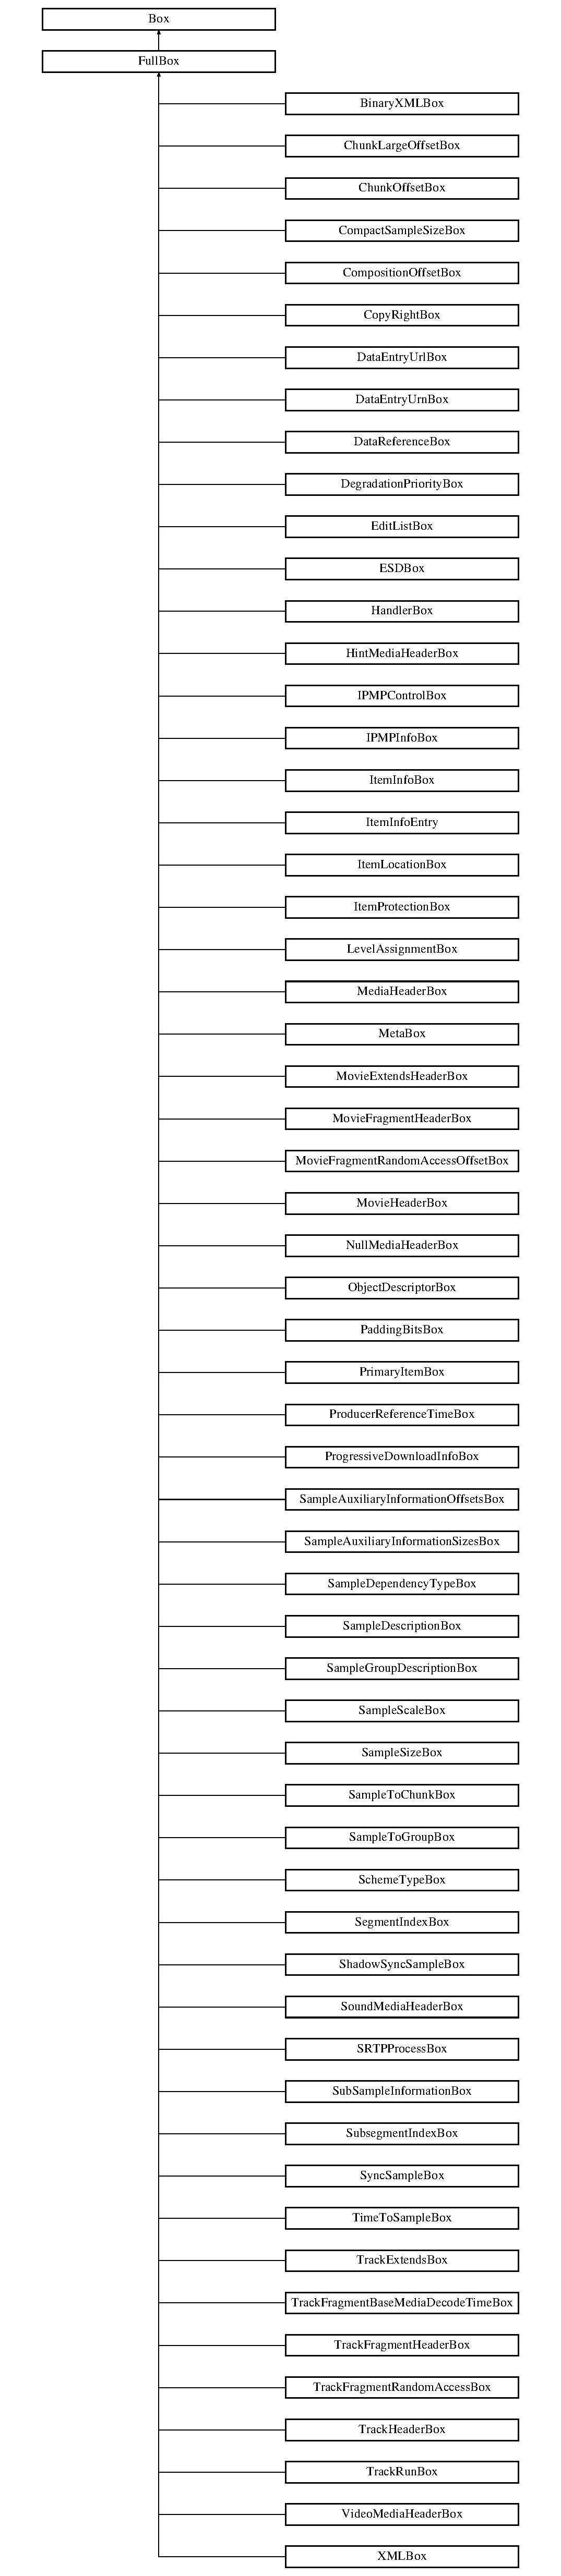
\includegraphics[height=12.000000cm]{class_full_box}
\end{center}
\end{figure}
\subsection*{Public Member Functions}
\begin{DoxyCompactItemize}
\item 
\hypertarget{class_full_box_a1dd227d6afcfddbd4bc5c4018e339858}{{\bfseries Full\-Box} (const unsigned long int \&s, const Q\-String \&t, const unsigned long int \&off, const unsigned int \&v, const Q\-List$<$ unsigned int $>$ \&f)}\label{class_full_box_a1dd227d6afcfddbd4bc5c4018e339858}

\item 
virtual Q\-String \hyperlink{class_full_box_a0701464d8e7386653f025833308f76ee}{get\-Full\-Name} ()
\begin{DoxyCompactList}\small\item\em get\-Full\-Name \end{DoxyCompactList}\item 
\hypertarget{class_full_box_afc93cc08ed7bc9b30ed219fd9b29d8a6}{unsigned int {\bfseries get\-Version} ()}\label{class_full_box_afc93cc08ed7bc9b30ed219fd9b29d8a6}

\item 
\hypertarget{class_full_box_a3569e34dffcdf998407fc2a77e5beb63}{Q\-List$<$ unsigned int $>$ {\bfseries get\-Flags} ()}\label{class_full_box_a3569e34dffcdf998407fc2a77e5beb63}

\end{DoxyCompactItemize}
\subsection*{Protected Attributes}
\begin{DoxyCompactItemize}
\item 
\hypertarget{class_full_box_a1fcf373fb0a760b702c02c20c18bb089}{unsigned int \hyperlink{class_full_box_a1fcf373fb0a760b702c02c20c18bb089}{version}}\label{class_full_box_a1fcf373fb0a760b702c02c20c18bb089}

\begin{DoxyCompactList}\small\item\em version indicates version of \hyperlink{class_full_box}{Full\-Box}. When set to 1, some of the paramaters can have bigger size (64-\/bit instead of 32-\/bit) \end{DoxyCompactList}\item 
\hypertarget{class_full_box_a3bfedd3ddb29af4762e0ef40c4c6830b}{Q\-List$<$ unsigned int $>$ \hyperlink{class_full_box_a3bfedd3ddb29af4762e0ef40c4c6830b}{flags}}\label{class_full_box_a3bfedd3ddb29af4762e0ef40c4c6830b}

\begin{DoxyCompactList}\small\item\em flags 3 unsigned int numbers that can determine forward content of the box or meaning of the other attributes. \end{DoxyCompactList}\end{DoxyCompactItemize}


\subsection{Detailed Description}
The \hyperlink{class_full_box}{Full\-Box} class represents Full \hyperlink{class_box}{Box}. 

\begin{DoxySeeAlso}{See Also}
I\-S\-O/\-I\-E\-C 14496-\/12 Information technology – Coding of audio-\/visual objects – Part 12\-: I\-S\-O base media file format 
\end{DoxySeeAlso}


\subsection{Member Function Documentation}
\hypertarget{class_full_box_a0701464d8e7386653f025833308f76ee}{\index{Full\-Box@{Full\-Box}!get\-Full\-Name@{get\-Full\-Name}}
\index{get\-Full\-Name@{get\-Full\-Name}!FullBox@{Full\-Box}}
\subsubsection[{get\-Full\-Name}]{\setlength{\rightskip}{0pt plus 5cm}virtual Q\-String Full\-Box\-::get\-Full\-Name (
\begin{DoxyParamCaption}
{}
\end{DoxyParamCaption}
)\hspace{0.3cm}{\ttfamily [inline]}, {\ttfamily [virtual]}}}\label{class_full_box_a0701464d8e7386653f025833308f76ee}


get\-Full\-Name 

\begin{DoxyReturn}{Returns}
full\-Name of the box, e.\-g. \char`\"{}\-Media Data Box\char`\"{} 
\end{DoxyReturn}


Reimplemented from \hyperlink{class_box_aa7c1e41e425cce53e0bd532cfafbb67d}{Box}.



Reimplemented in \hyperlink{class_padding_bits_box_ab355f0ebfa4a84ef4a2737bc9c264004}{Padding\-Bits\-Box}, \hyperlink{class_degradation_priority_box_a97f91434e74e47bc9e10ff9a21dd3023}{Degradation\-Priority\-Box}, \hyperlink{class_shadow_sync_sample_box_ab6644ef80649f21ac098f0d78904e9df}{Shadow\-Sync\-Sample\-Box}, \hyperlink{class_sync_sample_box_a9d3ab6e8730ca0cca633b7920e131413}{Sync\-Sample\-Box}, \hyperlink{class_handler_box_a77b90ca0801113aed5f6272035da0a04}{Handler\-Box}, \hyperlink{class_chunk_large_offset_box_acdadc159668e5e6ab286dbb840877f31}{Chunk\-Large\-Offset\-Box}, \hyperlink{class_track_fragment_base_media_decode_time_box_acf81a553080878b3066b24fc00b14f9e}{Track\-Fragment\-Base\-Media\-Decode\-Time\-Box}, \hyperlink{class_chunk_offset_box_a1c26ce6ada45f85c65761ed27f382848}{Chunk\-Offset\-Box}, \hyperlink{class_track_fragment_random_access_box_afeb1c2b67373428008a209cf01f6df10}{Track\-Fragment\-Random\-Access\-Box}, \hyperlink{class_e_s_d_box_a9e610dce6e72228e08fcbdfca0177c85}{E\-S\-D\-Box}, \hyperlink{class_sample_to_chunk_box_a298e53e6d563e66b7b910f99caeac0c3}{Sample\-To\-Chunk\-Box}, \hyperlink{class_track_run_box_a26fb4feae53dac2aa48caaa39ccceb81}{Track\-Run\-Box}, \hyperlink{class_object_descriptor_box_ae01792b840bd4547ecc0aba4ee665998}{Object\-Descriptor\-Box}, \hyperlink{class_compact_sample_size_box_a10c8ab4b452dd5c2d58e2c744ffac884}{Compact\-Sample\-Size\-Box}, \hyperlink{class_track_fragment_header_box_a6868fba2faed6053702b3c70751195e2}{Track\-Fragment\-Header\-Box}, \hyperlink{class_sample_size_box_a3cdb87618bba15d0c9e8cea9dde19ee5}{Sample\-Size\-Box}, \hyperlink{class_track_extends_box_acaa1a49911d86e5ca02ce2038398ff5d}{Track\-Extends\-Box}, \hyperlink{class_sample_description_box_a47754fb62da6522d13ff58de1ede0f09}{Sample\-Description\-Box}, \hyperlink{class_composition_offset_box_a6ed0d84212f70f61a021b39e1114c0fb}{Composition\-Offset\-Box}, \hyperlink{class_track_header_box_a7bc710a767026e2128ae46a1d3302778}{Track\-Header\-Box}, and \hyperlink{class_time_to_sample_box_a44c8086a9f61fb72f9549e8f997be7b9}{Time\-To\-Sample\-Box}.



The documentation for this class was generated from the following files\-:\begin{DoxyCompactItemize}
\item 
Model/\-Boxes/box.\-h\item 
Model/\-Boxes/box.\-cpp\end{DoxyCompactItemize}

\hypertarget{class_handler_box}{\section{Handler\-Box Class Reference}
\label{class_handler_box}\index{Handler\-Box@{Handler\-Box}}
}


The \hyperlink{class_handler_box}{Handler\-Box} class represents 'hdlr' box.  




{\ttfamily \#include $<$trackbox.\-h$>$}

Inheritance diagram for Handler\-Box\-:\begin{figure}[H]
\begin{center}
\leavevmode
\includegraphics[height=3.000000cm]{class_handler_box}
\end{center}
\end{figure}
\subsection*{Public Member Functions}
\begin{DoxyCompactItemize}
\item 
\hypertarget{class_handler_box_ad1069caa75de739c4499ff77418fffb8}{{\bfseries Handler\-Box} (const unsigned int \&s, const Q\-String \&t, const unsigned long int \&off, const unsigned int \&v, const Q\-List$<$ unsigned int $>$ \&f, const unsigned int \&pred, const unsigned int \&hand, const Q\-List$<$ unsigned int $>$ \&res, const Q\-String \&nam)}\label{class_handler_box_ad1069caa75de739c4499ff77418fffb8}

\item 
virtual Q\-String \hyperlink{class_handler_box_a77b90ca0801113aed5f6272035da0a04}{get\-Full\-Name} ()
\begin{DoxyCompactList}\small\item\em get\-Full\-Name \end{DoxyCompactList}\item 
virtual Q\-Standard\-Item\-Model $\ast$ \hyperlink{class_handler_box_a3d0550ec682df1ea81856082f431bc28}{get\-Model} ()
\begin{DoxyCompactList}\small\item\em get\-Model Constructs and return Q\-Standard\-Item\-Model object that is appropriate for graphical representation (for elements like Q\-Tree\-View, Q\-Table\-View etc.). Returned model contains names of the box attributes and their value. Each pair it's in its own row. Name of the attribute is in column 0, value -\/ column 1. \end{DoxyCompactList}\end{DoxyCompactItemize}
\subsection*{Protected Attributes}
\begin{DoxyCompactItemize}
\item 
\hypertarget{class_handler_box_a75290b7e77971baba1230544d075d181}{unsigned int {\bfseries version}}\label{class_handler_box_a75290b7e77971baba1230544d075d181}

\item 
\hypertarget{class_handler_box_ac8d6fb255dda61138323555971f56ca9}{unsigned int {\bfseries predefined}}\label{class_handler_box_ac8d6fb255dda61138323555971f56ca9}

\item 
\hypertarget{class_handler_box_a425b38b548469f337591d4fcb1ff910c}{unsigned long int {\bfseries handler\-Type}}\label{class_handler_box_a425b38b548469f337591d4fcb1ff910c}

\item 
\hypertarget{class_handler_box_a53b9cfd0f9d8d43d65024c28ece584ea}{Q\-List$<$ unsigned int $>$ {\bfseries reserved}}\label{class_handler_box_a53b9cfd0f9d8d43d65024c28ece584ea}

\item 
\hypertarget{class_handler_box_af7343083076dec8d92d885099f7c11a0}{Q\-String {\bfseries name}}\label{class_handler_box_af7343083076dec8d92d885099f7c11a0}

\end{DoxyCompactItemize}


\subsection{Detailed Description}
The \hyperlink{class_handler_box}{Handler\-Box} class represents 'hdlr' box. 

\begin{DoxySeeAlso}{See Also}
I\-S\-O/\-I\-E\-C 14496-\/12 Information technology – Coding of audio-\/visual objects – Part 12\-: I\-S\-O base media file format 
\end{DoxySeeAlso}


\subsection{Member Function Documentation}
\hypertarget{class_handler_box_a77b90ca0801113aed5f6272035da0a04}{\index{Handler\-Box@{Handler\-Box}!get\-Full\-Name@{get\-Full\-Name}}
\index{get\-Full\-Name@{get\-Full\-Name}!HandlerBox@{Handler\-Box}}
\subsubsection[{get\-Full\-Name}]{\setlength{\rightskip}{0pt plus 5cm}virtual Q\-String Handler\-Box\-::get\-Full\-Name (
\begin{DoxyParamCaption}
{}
\end{DoxyParamCaption}
)\hspace{0.3cm}{\ttfamily [inline]}, {\ttfamily [virtual]}}}\label{class_handler_box_a77b90ca0801113aed5f6272035da0a04}


get\-Full\-Name 

\begin{DoxyReturn}{Returns}
full\-Name of the box, e.\-g. \char`\"{}\-Media Data Box\char`\"{} 
\end{DoxyReturn}


Reimplemented from \hyperlink{class_full_box_a0701464d8e7386653f025833308f76ee}{Full\-Box}.

\hypertarget{class_handler_box_a3d0550ec682df1ea81856082f431bc28}{\index{Handler\-Box@{Handler\-Box}!get\-Model@{get\-Model}}
\index{get\-Model@{get\-Model}!HandlerBox@{Handler\-Box}}
\subsubsection[{get\-Model}]{\setlength{\rightskip}{0pt plus 5cm}Q\-Standard\-Item\-Model $\ast$ Handler\-Box\-::get\-Model (
\begin{DoxyParamCaption}
{}
\end{DoxyParamCaption}
)\hspace{0.3cm}{\ttfamily [virtual]}}}\label{class_handler_box_a3d0550ec682df1ea81856082f431bc28}


get\-Model Constructs and return Q\-Standard\-Item\-Model object that is appropriate for graphical representation (for elements like Q\-Tree\-View, Q\-Table\-View etc.). Returned model contains names of the box attributes and their value. Each pair it's in its own row. Name of the attribute is in column 0, value -\/ column 1. 

\begin{DoxyReturn}{Returns}
model of \hyperlink{class_box}{Box} attributes 
\end{DoxyReturn}


Reimplemented from \hyperlink{class_box_a5c7911f3c88eec77383c0a464979807d}{Box}.



The documentation for this class was generated from the following files\-:\begin{DoxyCompactItemize}
\item 
Model/\-Boxes/trackbox.\-h\item 
Model/\-Boxes/trackbox.\-cpp\end{DoxyCompactItemize}

\hypertarget{class_hint_media_header_box}{\section{Hint\-Media\-Header\-Box Class Reference}
\label{class_hint_media_header_box}\index{Hint\-Media\-Header\-Box@{Hint\-Media\-Header\-Box}}
}


The \hyperlink{class_hint_media_header_box}{Hint\-Media\-Header\-Box} class represents 'hmhd' box.  




{\ttfamily \#include $<$box.\-h$>$}

Inheritance diagram for Hint\-Media\-Header\-Box\-:\begin{figure}[H]
\begin{center}
\leavevmode
\includegraphics[height=3.000000cm]{class_hint_media_header_box}
\end{center}
\end{figure}
\subsection*{Public Member Functions}
\begin{DoxyCompactItemize}
\item 
\hypertarget{class_hint_media_header_box_abdca8334746625953b8e3f13d2461048}{{\bfseries Hint\-Media\-Header\-Box} (const unsigned int \&s, const Q\-String \&t, const unsigned long int \&off, const unsigned int \&v, const Q\-List$<$ unsigned int $>$ \&f)}\label{class_hint_media_header_box_abdca8334746625953b8e3f13d2461048}

\item 
virtual Q\-String \hyperlink{class_hint_media_header_box_aacaa05edc0b37296c6b0cad9b216babe}{get\-Full\-Name} ()
\begin{DoxyCompactList}\small\item\em get\-Full\-Name \end{DoxyCompactList}\end{DoxyCompactItemize}
\subsection*{Additional Inherited Members}


\subsection{Detailed Description}
The \hyperlink{class_hint_media_header_box}{Hint\-Media\-Header\-Box} class represents 'hmhd' box. 

\begin{DoxySeeAlso}{See Also}
I\-S\-O/\-I\-E\-C 14496-\/12 Information technology – Coding of audio-\/visual objects – Part 12\-: I\-S\-O base media file format 
\end{DoxySeeAlso}


\subsection{Member Function Documentation}
\hypertarget{class_hint_media_header_box_aacaa05edc0b37296c6b0cad9b216babe}{\index{Hint\-Media\-Header\-Box@{Hint\-Media\-Header\-Box}!get\-Full\-Name@{get\-Full\-Name}}
\index{get\-Full\-Name@{get\-Full\-Name}!HintMediaHeaderBox@{Hint\-Media\-Header\-Box}}
\subsubsection[{get\-Full\-Name}]{\setlength{\rightskip}{0pt plus 5cm}virtual Q\-String Hint\-Media\-Header\-Box\-::get\-Full\-Name (
\begin{DoxyParamCaption}
{}
\end{DoxyParamCaption}
)\hspace{0.3cm}{\ttfamily [inline]}, {\ttfamily [virtual]}}}\label{class_hint_media_header_box_aacaa05edc0b37296c6b0cad9b216babe}


get\-Full\-Name 

\begin{DoxyReturn}{Returns}
full\-Name of the box, e.\-g. \char`\"{}\-Media Data Box\char`\"{} 
\end{DoxyReturn}


Reimplemented from \hyperlink{class_full_box_a0701464d8e7386653f025833308f76ee}{Full\-Box}.



The documentation for this class was generated from the following files\-:\begin{DoxyCompactItemize}
\item 
Model/\-Boxes/box.\-h\item 
Model/\-Boxes/box.\-cpp\end{DoxyCompactItemize}

\hypertarget{class_hint_sample_entry}{\section{Hint\-Sample\-Entry Class Reference}
\label{class_hint_sample_entry}\index{Hint\-Sample\-Entry@{Hint\-Sample\-Entry}}
}


The \hyperlink{class_hint_sample_entry}{Hint\-Sample\-Entry} class represents Hint Sample Entry Class.  




{\ttfamily \#include $<$sampleentry.\-h$>$}

Inheritance diagram for Hint\-Sample\-Entry\-:\begin{figure}[H]
\begin{center}
\leavevmode
\includegraphics[height=3.000000cm]{class_hint_sample_entry}
\end{center}
\end{figure}
\subsection*{Public Member Functions}
\begin{DoxyCompactItemize}
\item 
\hypertarget{class_hint_sample_entry_ad981306f2f9352416a0657cc2eaa8668}{{\bfseries Hint\-Sample\-Entry} (const unsigned long int \&s, const Q\-String \&t, const unsigned long int \&off, const Q\-List$<$ unsigned int $>$ \&res, const unsigned int \&dri)}\label{class_hint_sample_entry_ad981306f2f9352416a0657cc2eaa8668}

\item 
virtual Q\-String \hyperlink{class_hint_sample_entry_ac747c305de54a619efe66d5d8e0ec61a}{get\-Full\-Name} ()
\begin{DoxyCompactList}\small\item\em get\-Full\-Name \end{DoxyCompactList}\end{DoxyCompactItemize}
\subsection*{Additional Inherited Members}


\subsection{Detailed Description}
The \hyperlink{class_hint_sample_entry}{Hint\-Sample\-Entry} class represents Hint Sample Entry Class. 

\begin{DoxySeeAlso}{See Also}
I\-S\-O/\-I\-E\-C 14496-\/12 Information technology – Coding of audio-\/visual objects – Part 12\-: I\-S\-O base media file format 
\end{DoxySeeAlso}


\subsection{Member Function Documentation}
\hypertarget{class_hint_sample_entry_ac747c305de54a619efe66d5d8e0ec61a}{\index{Hint\-Sample\-Entry@{Hint\-Sample\-Entry}!get\-Full\-Name@{get\-Full\-Name}}
\index{get\-Full\-Name@{get\-Full\-Name}!HintSampleEntry@{Hint\-Sample\-Entry}}
\subsubsection[{get\-Full\-Name}]{\setlength{\rightskip}{0pt plus 5cm}virtual Q\-String Hint\-Sample\-Entry\-::get\-Full\-Name (
\begin{DoxyParamCaption}
{}
\end{DoxyParamCaption}
)\hspace{0.3cm}{\ttfamily [inline]}, {\ttfamily [virtual]}}}\label{class_hint_sample_entry_ac747c305de54a619efe66d5d8e0ec61a}


get\-Full\-Name 

\begin{DoxyReturn}{Returns}
full\-Name of the box, e.\-g. \char`\"{}\-Media Data Box\char`\"{} 
\end{DoxyReturn}


Reimplemented from \hyperlink{class_sample_entry_acbc7081715759b868797ad71b469a63e}{Sample\-Entry}.



The documentation for this class was generated from the following files\-:\begin{DoxyCompactItemize}
\item 
Model/\-Boxes/sampleentry.\-h\item 
Model/\-Boxes/sampleentry.\-cpp\end{DoxyCompactItemize}

\hypertarget{class_hint_statistics_box}{\section{Hint\-Statistics\-Box Class Reference}
\label{class_hint_statistics_box}\index{Hint\-Statistics\-Box@{Hint\-Statistics\-Box}}
}


The \hyperlink{class_hint_statistics_box}{Hint\-Statistics\-Box} class represents 'hinf' box.  




{\ttfamily \#include $<$box.\-h$>$}

Inheritance diagram for Hint\-Statistics\-Box\-:\begin{figure}[H]
\begin{center}
\leavevmode
\includegraphics[height=2.000000cm]{class_hint_statistics_box}
\end{center}
\end{figure}
\subsection*{Public Member Functions}
\begin{DoxyCompactItemize}
\item 
\hypertarget{class_hint_statistics_box_a31d6a7f3945b501f5e77b0c735ddfbe2}{{\bfseries Hint\-Statistics\-Box} (const unsigned int \&s, const Q\-String \&t, const unsigned long int \&off)}\label{class_hint_statistics_box_a31d6a7f3945b501f5e77b0c735ddfbe2}

\item 
virtual Q\-String \hyperlink{class_hint_statistics_box_acec0896d250145c53576fb9f079136ca}{get\-Full\-Name} ()
\begin{DoxyCompactList}\small\item\em get\-Full\-Name \end{DoxyCompactList}\end{DoxyCompactItemize}
\subsection*{Additional Inherited Members}


\subsection{Detailed Description}
The \hyperlink{class_hint_statistics_box}{Hint\-Statistics\-Box} class represents 'hinf' box. 

\begin{DoxySeeAlso}{See Also}
I\-S\-O/\-I\-E\-C 14496-\/12 Information technology – Coding of audio-\/visual objects – Part 12\-: I\-S\-O base media file format 
\end{DoxySeeAlso}


\subsection{Member Function Documentation}
\hypertarget{class_hint_statistics_box_acec0896d250145c53576fb9f079136ca}{\index{Hint\-Statistics\-Box@{Hint\-Statistics\-Box}!get\-Full\-Name@{get\-Full\-Name}}
\index{get\-Full\-Name@{get\-Full\-Name}!HintStatisticsBox@{Hint\-Statistics\-Box}}
\subsubsection[{get\-Full\-Name}]{\setlength{\rightskip}{0pt plus 5cm}virtual Q\-String Hint\-Statistics\-Box\-::get\-Full\-Name (
\begin{DoxyParamCaption}
{}
\end{DoxyParamCaption}
)\hspace{0.3cm}{\ttfamily [inline]}, {\ttfamily [virtual]}}}\label{class_hint_statistics_box_acec0896d250145c53576fb9f079136ca}


get\-Full\-Name 

\begin{DoxyReturn}{Returns}
full\-Name of the box, e.\-g. \char`\"{}\-Media Data Box\char`\"{} 
\end{DoxyReturn}


Reimplemented from \hyperlink{class_box_aa7c1e41e425cce53e0bd532cfafbb67d}{Box}.



The documentation for this class was generated from the following files\-:\begin{DoxyCompactItemize}
\item 
Model/\-Boxes/box.\-h\item 
Model/\-Boxes/box.\-cpp\end{DoxyCompactItemize}

\hypertarget{class_initialization}{\section{Initialization Class Reference}
\label{class_initialization}\index{Initialization@{Initialization}}
}


The \hyperlink{class_initialization}{Initialization} class represents \hyperlink{class_initialization}{Initialization} element of Media Presentation Description xml file.  




{\ttfamily \#include $<$segmentlist.\-h$>$}

\subsection*{Public Member Functions}
\begin{DoxyCompactItemize}
\item 
void \hyperlink{class_initialization_adbcec26db9b9b33a9b370875e656a93c}{write} (Q\-Xml\-Stream\-Writer $\ast$stream)
\begin{DoxyCompactList}\small\item\em write Writes \hyperlink{class_initialization}{Initialization} vertex into Media Presentation Description file \end{DoxyCompactList}\item 
\hypertarget{class_initialization_acb7cef5e5fd3b5c8efa67ec28097469f}{Q\-String {\bfseries get\-Range} () const }\label{class_initialization_acb7cef5e5fd3b5c8efa67ec28097469f}

\item 
\hypertarget{class_initialization_a82064f6832cf34a835ffef527d445c29}{void {\bfseries set\-Range} (const Q\-String \&value)}\label{class_initialization_a82064f6832cf34a835ffef527d445c29}

\item 
\hypertarget{class_initialization_a00fa04548517a51d0313a05250a12dab}{Q\-String {\bfseries get\-Source\-U\-R\-L} () const }\label{class_initialization_a00fa04548517a51d0313a05250a12dab}

\item 
\hypertarget{class_initialization_a82a2cf2f57099460d76de18bf3b9b6fe}{void {\bfseries set\-Source\-U\-R\-L} (const Q\-String \&value)}\label{class_initialization_a82a2cf2f57099460d76de18bf3b9b6fe}

\end{DoxyCompactItemize}


\subsection{Detailed Description}
The \hyperlink{class_initialization}{Initialization} class represents \hyperlink{class_initialization}{Initialization} element of Media Presentation Description xml file. 

\begin{DoxySeeAlso}{See Also}
I\-S\-O/\-I\-E\-C 23009-\/1\-:2012 Information technology – Dynamic adaptive streaming over H\-T\-T\-P (D\-A\-S\-H) – Part 1\-: Media presentation description and segment formats 
\end{DoxySeeAlso}


\subsection{Member Function Documentation}
\hypertarget{class_initialization_adbcec26db9b9b33a9b370875e656a93c}{\index{Initialization@{Initialization}!write@{write}}
\index{write@{write}!Initialization@{Initialization}}
\subsubsection[{write}]{\setlength{\rightskip}{0pt plus 5cm}void Initialization\-::write (
\begin{DoxyParamCaption}
\item[{Q\-Xml\-Stream\-Writer $\ast$}]{stream}
\end{DoxyParamCaption}
)}}\label{class_initialization_adbcec26db9b9b33a9b370875e656a93c}


write Writes \hyperlink{class_initialization}{Initialization} vertex into Media Presentation Description file 


\begin{DoxyParams}{Parameters}
{\em stream} & stream of the \hyperlink{class_m_p_d}{M\-P\-D} file \\
\hline
\end{DoxyParams}


The documentation for this class was generated from the following files\-:\begin{DoxyCompactItemize}
\item 
Model/\-Mpd/segmentlist.\-h\item 
Model/\-Mpd/segmentlist.\-cpp\end{DoxyCompactItemize}

\input{class_i_p_m_p_control_box}
\hypertarget{class_i_p_m_p_info_box}{\section{I\-P\-M\-P\-Info\-Box Class Reference}
\label{class_i_p_m_p_info_box}\index{I\-P\-M\-P\-Info\-Box@{I\-P\-M\-P\-Info\-Box}}
}


The \hyperlink{class_i_p_m_p_info_box}{I\-P\-M\-P\-Info\-Box} class represents 'imif' box.  




{\ttfamily \#include $<$box.\-h$>$}

Inheritance diagram for I\-P\-M\-P\-Info\-Box\-:\begin{figure}[H]
\begin{center}
\leavevmode
\includegraphics[height=3.000000cm]{class_i_p_m_p_info_box}
\end{center}
\end{figure}
\subsection*{Public Member Functions}
\begin{DoxyCompactItemize}
\item 
\hypertarget{class_i_p_m_p_info_box_aedab61143da41997c6dfc121a3982297}{{\bfseries I\-P\-M\-P\-Info\-Box} (const unsigned int \&s, const Q\-String \&t, const unsigned long int \&off, const unsigned int \&v, const Q\-List$<$ unsigned int $>$ \&f)}\label{class_i_p_m_p_info_box_aedab61143da41997c6dfc121a3982297}

\item 
virtual Q\-String \hyperlink{class_i_p_m_p_info_box_aef8ac41ff48a6fa3ce83f81dbdd369a1}{get\-Full\-Name} ()
\begin{DoxyCompactList}\small\item\em get\-Full\-Name \end{DoxyCompactList}\end{DoxyCompactItemize}
\subsection*{Additional Inherited Members}


\subsection{Detailed Description}
The \hyperlink{class_i_p_m_p_info_box}{I\-P\-M\-P\-Info\-Box} class represents 'imif' box. 

\begin{DoxySeeAlso}{See Also}
I\-S\-O/\-I\-E\-C 14496-\/12 Information technology – Coding of audio-\/visual objects – Part 12\-: I\-S\-O base media file format 
\end{DoxySeeAlso}


\subsection{Member Function Documentation}
\hypertarget{class_i_p_m_p_info_box_aef8ac41ff48a6fa3ce83f81dbdd369a1}{\index{I\-P\-M\-P\-Info\-Box@{I\-P\-M\-P\-Info\-Box}!get\-Full\-Name@{get\-Full\-Name}}
\index{get\-Full\-Name@{get\-Full\-Name}!IPMPInfoBox@{I\-P\-M\-P\-Info\-Box}}
\subsubsection[{get\-Full\-Name}]{\setlength{\rightskip}{0pt plus 5cm}virtual Q\-String I\-P\-M\-P\-Info\-Box\-::get\-Full\-Name (
\begin{DoxyParamCaption}
{}
\end{DoxyParamCaption}
)\hspace{0.3cm}{\ttfamily [inline]}, {\ttfamily [virtual]}}}\label{class_i_p_m_p_info_box_aef8ac41ff48a6fa3ce83f81dbdd369a1}


get\-Full\-Name 

\begin{DoxyReturn}{Returns}
full\-Name of the box, e.\-g. \char`\"{}\-Media Data Box\char`\"{} 
\end{DoxyReturn}


Reimplemented from \hyperlink{class_full_box_a0701464d8e7386653f025833308f76ee}{Full\-Box}.



The documentation for this class was generated from the following files\-:\begin{DoxyCompactItemize}
\item 
Model/\-Boxes/box.\-h\item 
Model/\-Boxes/box.\-cpp\end{DoxyCompactItemize}

\hypertarget{class_item_info_box}{\section{Item\-Info\-Box Class Reference}
\label{class_item_info_box}\index{Item\-Info\-Box@{Item\-Info\-Box}}
}


The \hyperlink{class_item_info_box}{Item\-Info\-Box} class represents 'iinf' box.  




{\ttfamily \#include $<$box.\-h$>$}

Inheritance diagram for Item\-Info\-Box\-:\begin{figure}[H]
\begin{center}
\leavevmode
\includegraphics[height=3.000000cm]{class_item_info_box}
\end{center}
\end{figure}
\subsection*{Public Member Functions}
\begin{DoxyCompactItemize}
\item 
\hypertarget{class_item_info_box_a8325c989bebeace0d276f118b95705e0}{{\bfseries Item\-Info\-Box} (const unsigned int \&s, const Q\-String \&t, const unsigned long int \&off, const unsigned int \&v, const Q\-List$<$ unsigned int $>$ \&f)}\label{class_item_info_box_a8325c989bebeace0d276f118b95705e0}

\item 
virtual Q\-String \hyperlink{class_item_info_box_acc8b801d684beee63b12ea00aa84b1d4}{get\-Full\-Name} ()
\begin{DoxyCompactList}\small\item\em get\-Full\-Name \end{DoxyCompactList}\end{DoxyCompactItemize}
\subsection*{Additional Inherited Members}


\subsection{Detailed Description}
The \hyperlink{class_item_info_box}{Item\-Info\-Box} class represents 'iinf' box. 

\begin{DoxySeeAlso}{See Also}
I\-S\-O/\-I\-E\-C 14496-\/12 Information technology – Coding of audio-\/visual objects – Part 12\-: I\-S\-O base media file format 
\end{DoxySeeAlso}


\subsection{Member Function Documentation}
\hypertarget{class_item_info_box_acc8b801d684beee63b12ea00aa84b1d4}{\index{Item\-Info\-Box@{Item\-Info\-Box}!get\-Full\-Name@{get\-Full\-Name}}
\index{get\-Full\-Name@{get\-Full\-Name}!ItemInfoBox@{Item\-Info\-Box}}
\subsubsection[{get\-Full\-Name}]{\setlength{\rightskip}{0pt plus 5cm}virtual Q\-String Item\-Info\-Box\-::get\-Full\-Name (
\begin{DoxyParamCaption}
{}
\end{DoxyParamCaption}
)\hspace{0.3cm}{\ttfamily [inline]}, {\ttfamily [virtual]}}}\label{class_item_info_box_acc8b801d684beee63b12ea00aa84b1d4}


get\-Full\-Name 

\begin{DoxyReturn}{Returns}
full\-Name of the box, e.\-g. \char`\"{}\-Media Data Box\char`\"{} 
\end{DoxyReturn}


Reimplemented from \hyperlink{class_full_box_a0701464d8e7386653f025833308f76ee}{Full\-Box}.



The documentation for this class was generated from the following files\-:\begin{DoxyCompactItemize}
\item 
Model/\-Boxes/box.\-h\item 
Model/\-Boxes/box.\-cpp\end{DoxyCompactItemize}

\hypertarget{class_item_info_entry}{\section{Item\-Info\-Entry Class Reference}
\label{class_item_info_entry}\index{Item\-Info\-Entry@{Item\-Info\-Entry}}
}


The \hyperlink{class_item_info_entry}{Item\-Info\-Entry} class represents 'infe' box.  




{\ttfamily \#include $<$box.\-h$>$}

Inheritance diagram for Item\-Info\-Entry\-:\begin{figure}[H]
\begin{center}
\leavevmode
\includegraphics[height=3.000000cm]{class_item_info_entry}
\end{center}
\end{figure}
\subsection*{Public Member Functions}
\begin{DoxyCompactItemize}
\item 
\hypertarget{class_item_info_entry_a0f977408181457a930b5a32d662ce183}{{\bfseries Item\-Info\-Entry} (const unsigned int \&s, const Q\-String \&t, const unsigned long int \&off, const unsigned int \&v, const Q\-List$<$ unsigned int $>$ \&f)}\label{class_item_info_entry_a0f977408181457a930b5a32d662ce183}

\item 
virtual Q\-String \hyperlink{class_item_info_entry_a7d744fa6aeb0ee948a898bb7b629a384}{get\-Full\-Name} ()
\begin{DoxyCompactList}\small\item\em get\-Full\-Name \end{DoxyCompactList}\end{DoxyCompactItemize}
\subsection*{Additional Inherited Members}


\subsection{Detailed Description}
The \hyperlink{class_item_info_entry}{Item\-Info\-Entry} class represents 'infe' box. 

\begin{DoxySeeAlso}{See Also}
I\-S\-O/\-I\-E\-C 14496-\/12 Information technology – Coding of audio-\/visual objects – Part 12\-: I\-S\-O base media file format 
\end{DoxySeeAlso}


\subsection{Member Function Documentation}
\hypertarget{class_item_info_entry_a7d744fa6aeb0ee948a898bb7b629a384}{\index{Item\-Info\-Entry@{Item\-Info\-Entry}!get\-Full\-Name@{get\-Full\-Name}}
\index{get\-Full\-Name@{get\-Full\-Name}!ItemInfoEntry@{Item\-Info\-Entry}}
\subsubsection[{get\-Full\-Name}]{\setlength{\rightskip}{0pt plus 5cm}virtual Q\-String Item\-Info\-Entry\-::get\-Full\-Name (
\begin{DoxyParamCaption}
{}
\end{DoxyParamCaption}
)\hspace{0.3cm}{\ttfamily [inline]}, {\ttfamily [virtual]}}}\label{class_item_info_entry_a7d744fa6aeb0ee948a898bb7b629a384}


get\-Full\-Name 

\begin{DoxyReturn}{Returns}
full\-Name of the box, e.\-g. \char`\"{}\-Media Data Box\char`\"{} 
\end{DoxyReturn}


Reimplemented from \hyperlink{class_full_box_a0701464d8e7386653f025833308f76ee}{Full\-Box}.



The documentation for this class was generated from the following files\-:\begin{DoxyCompactItemize}
\item 
Model/\-Boxes/box.\-h\item 
Model/\-Boxes/box.\-cpp\end{DoxyCompactItemize}

\hypertarget{class_item_location_box}{\section{Item\-Location\-Box Class Reference}
\label{class_item_location_box}\index{Item\-Location\-Box@{Item\-Location\-Box}}
}


The \hyperlink{class_item_location_box}{Item\-Location\-Box} class represents 'iloc' box.  




{\ttfamily \#include $<$box.\-h$>$}

Inheritance diagram for Item\-Location\-Box\-:\begin{figure}[H]
\begin{center}
\leavevmode
\includegraphics[height=3.000000cm]{class_item_location_box}
\end{center}
\end{figure}
\subsection*{Public Member Functions}
\begin{DoxyCompactItemize}
\item 
\hypertarget{class_item_location_box_ac474e27389e8141b00ea61cd1a5f9d1b}{{\bfseries Item\-Location\-Box} (const unsigned int \&s, const Q\-String \&t, const unsigned long int \&off, const unsigned int \&v, const Q\-List$<$ unsigned int $>$ \&f)}\label{class_item_location_box_ac474e27389e8141b00ea61cd1a5f9d1b}

\item 
virtual Q\-String \hyperlink{class_item_location_box_a88ae4bd69cdcc39a4f54b894631c12fe}{get\-Full\-Name} ()
\begin{DoxyCompactList}\small\item\em get\-Full\-Name \end{DoxyCompactList}\end{DoxyCompactItemize}
\subsection*{Additional Inherited Members}


\subsection{Detailed Description}
The \hyperlink{class_item_location_box}{Item\-Location\-Box} class represents 'iloc' box. 

\begin{DoxySeeAlso}{See Also}
I\-S\-O/\-I\-E\-C 14496-\/12 Information technology – Coding of audio-\/visual objects – Part 12\-: I\-S\-O base media file format 
\end{DoxySeeAlso}


\subsection{Member Function Documentation}
\hypertarget{class_item_location_box_a88ae4bd69cdcc39a4f54b894631c12fe}{\index{Item\-Location\-Box@{Item\-Location\-Box}!get\-Full\-Name@{get\-Full\-Name}}
\index{get\-Full\-Name@{get\-Full\-Name}!ItemLocationBox@{Item\-Location\-Box}}
\subsubsection[{get\-Full\-Name}]{\setlength{\rightskip}{0pt plus 5cm}virtual Q\-String Item\-Location\-Box\-::get\-Full\-Name (
\begin{DoxyParamCaption}
{}
\end{DoxyParamCaption}
)\hspace{0.3cm}{\ttfamily [inline]}, {\ttfamily [virtual]}}}\label{class_item_location_box_a88ae4bd69cdcc39a4f54b894631c12fe}


get\-Full\-Name 

\begin{DoxyReturn}{Returns}
full\-Name of the box, e.\-g. \char`\"{}\-Media Data Box\char`\"{} 
\end{DoxyReturn}


Reimplemented from \hyperlink{class_full_box_a0701464d8e7386653f025833308f76ee}{Full\-Box}.



The documentation for this class was generated from the following files\-:\begin{DoxyCompactItemize}
\item 
Model/\-Boxes/box.\-h\item 
Model/\-Boxes/box.\-cpp\end{DoxyCompactItemize}

\hypertarget{class_item_protection_box}{\section{Item\-Protection\-Box Class Reference}
\label{class_item_protection_box}\index{Item\-Protection\-Box@{Item\-Protection\-Box}}
}


The \hyperlink{class_item_protection_box}{Item\-Protection\-Box} class represents 'ipro' box.  




{\ttfamily \#include $<$box.\-h$>$}

Inheritance diagram for Item\-Protection\-Box\-:\begin{figure}[H]
\begin{center}
\leavevmode
\includegraphics[height=3.000000cm]{class_item_protection_box}
\end{center}
\end{figure}
\subsection*{Public Member Functions}
\begin{DoxyCompactItemize}
\item 
\hypertarget{class_item_protection_box_ac9688520f3d4da689467b2e72df74b08}{{\bfseries Item\-Protection\-Box} (const unsigned int \&s, const Q\-String \&t, const unsigned long int \&off, const unsigned int \&v, const Q\-List$<$ unsigned int $>$ \&f)}\label{class_item_protection_box_ac9688520f3d4da689467b2e72df74b08}

\item 
virtual bool \hyperlink{class_item_protection_box_a3d1db2ceacc95601edf25808f3bcf4c3}{is\-Container} ()
\begin{DoxyCompactList}\small\item\em is\-Container \end{DoxyCompactList}\item 
virtual Q\-String \hyperlink{class_item_protection_box_a282908379f31aeaacb0eac073050b132}{get\-Full\-Name} ()
\begin{DoxyCompactList}\small\item\em get\-Full\-Name \end{DoxyCompactList}\end{DoxyCompactItemize}
\subsection*{Additional Inherited Members}


\subsection{Detailed Description}
The \hyperlink{class_item_protection_box}{Item\-Protection\-Box} class represents 'ipro' box. 

\begin{DoxySeeAlso}{See Also}
I\-S\-O/\-I\-E\-C 14496-\/12 Information technology – Coding of audio-\/visual objects – Part 12\-: I\-S\-O base media file format 
\end{DoxySeeAlso}


\subsection{Member Function Documentation}
\hypertarget{class_item_protection_box_a282908379f31aeaacb0eac073050b132}{\index{Item\-Protection\-Box@{Item\-Protection\-Box}!get\-Full\-Name@{get\-Full\-Name}}
\index{get\-Full\-Name@{get\-Full\-Name}!ItemProtectionBox@{Item\-Protection\-Box}}
\subsubsection[{get\-Full\-Name}]{\setlength{\rightskip}{0pt plus 5cm}virtual Q\-String Item\-Protection\-Box\-::get\-Full\-Name (
\begin{DoxyParamCaption}
{}
\end{DoxyParamCaption}
)\hspace{0.3cm}{\ttfamily [inline]}, {\ttfamily [virtual]}}}\label{class_item_protection_box_a282908379f31aeaacb0eac073050b132}


get\-Full\-Name 

\begin{DoxyReturn}{Returns}
full\-Name of the box, e.\-g. \char`\"{}\-Media Data Box\char`\"{} 
\end{DoxyReturn}


Reimplemented from \hyperlink{class_full_box_a0701464d8e7386653f025833308f76ee}{Full\-Box}.

\hypertarget{class_item_protection_box_a3d1db2ceacc95601edf25808f3bcf4c3}{\index{Item\-Protection\-Box@{Item\-Protection\-Box}!is\-Container@{is\-Container}}
\index{is\-Container@{is\-Container}!ItemProtectionBox@{Item\-Protection\-Box}}
\subsubsection[{is\-Container}]{\setlength{\rightskip}{0pt plus 5cm}virtual bool Item\-Protection\-Box\-::is\-Container (
\begin{DoxyParamCaption}
{}
\end{DoxyParamCaption}
)\hspace{0.3cm}{\ttfamily [inline]}, {\ttfamily [virtual]}}}\label{class_item_protection_box_a3d1db2ceacc95601edf25808f3bcf4c3}


is\-Container 

\begin{DoxyReturn}{Returns}
true when box contains other boxes, false otherwise 
\end{DoxyReturn}


Reimplemented from \hyperlink{class_box_aa836717b34b2a26f84b6933d143da42b}{Box}.



The documentation for this class was generated from the following files\-:\begin{DoxyCompactItemize}
\item 
Model/\-Boxes/box.\-h\item 
Model/\-Boxes/box.\-cpp\end{DoxyCompactItemize}

\input{class_level_assignment_box}
\hypertarget{class_main_window}{\section{Main\-Window Class Reference}
\label{class_main_window}\index{Main\-Window@{Main\-Window}}
}


The \hyperlink{class_main_window}{Main\-Window} class defines a main window of the application.  




{\ttfamily \#include $<$mainwindow.\-h$>$}

Inheritance diagram for Main\-Window\-:\begin{figure}[H]
\begin{center}
\leavevmode
\includegraphics[height=2.000000cm]{class_main_window}
\end{center}
\end{figure}
\subsection*{Signals}
\begin{DoxyCompactItemize}
\item 
void \hyperlink{class_main_window_a49edf26b374679e5569a25de2f05ab87}{file\-Selected} (const Q\-String \&file\-Name)
\begin{DoxyCompactList}\small\item\em file\-Selected \end{DoxyCompactList}\item 
void \hyperlink{class_main_window_adc10d5521d5f7c43a57fceb4e2a5953e}{box\-Selected} (Q\-Item\-Selection\-Model $\ast$selection)
\begin{DoxyCompactList}\small\item\em box\-Selected \end{DoxyCompactList}\item 
void \hyperlink{class_main_window_add6f50ee0cfda97372eea9fbfea8f09b}{search\-Box} (const Q\-String \&box\-Type)
\begin{DoxyCompactList}\small\item\em search\-Box \end{DoxyCompactList}\item 
void \hyperlink{class_main_window_a3cacf65545a464647562b468a0e08f36}{dash\-Files\-Selected\-Signal} (const bool \&one\-File, const Q\-String \&url)
\begin{DoxyCompactList}\small\item\em dash\-Files\-Selected\-Signal \end{DoxyCompactList}\item 
void \hyperlink{class_main_window_ab20d195ebd6ecf001235d88f1c7c680b}{dash\-Dir\-Selected\-Sig} (const Q\-String \&dir)
\begin{DoxyCompactList}\small\item\em dash\-Dir\-Selected\-Sig \end{DoxyCompactList}\item 
void \hyperlink{class_main_window_a9afe6d97db65fe1cdff622187fbb86bc}{remove\-File\-Sig} (const int \&row)
\begin{DoxyCompactList}\small\item\em remove\-File\-Sig \end{DoxyCompactList}\end{DoxyCompactItemize}
\subsection*{Public Member Functions}
\begin{DoxyCompactItemize}
\item 
\hyperlink{class_main_window_a8b244be8b7b7db1b08de2a2acb9409db}{Main\-Window} (Q\-Widget $\ast$parent=0)
\begin{DoxyCompactList}\small\item\em \hyperlink{class_main_window}{Main\-Window} Constructor of \hyperlink{class_main_window}{Main\-Window}. \end{DoxyCompactList}\item 
void \hyperlink{class_main_window_a9757b11e83740195027a8fe486e9f221}{file\-Analyzed} (\hyperlink{class_tree_model}{Tree\-Model} $\ast$model, const Q\-String \&file\-Name)
\begin{DoxyCompactList}\small\item\em file\-Analyzed \end{DoxyCompactList}\item 
void \hyperlink{class_main_window_a8a8ff9ef51b23c7fff3102ae6c0f5fdf}{print\-Selected\-Box} (Q\-Standard\-Item\-Model $\ast$model, \hyperlink{class_tree_item}{Tree\-Item} $\ast$item)
\begin{DoxyCompactList}\small\item\em print\-Selected\-Box \end{DoxyCompactList}\item 
void \hyperlink{class_main_window_a199be1af8e0e67ce6b8cba1f16985419}{select\-Boxes\-Found} (Q\-Model\-Index\-List \&boxes, const Q\-String \&full\-Name)
\begin{DoxyCompactList}\small\item\em select\-Boxes\-Found \end{DoxyCompactList}\item 
void \hyperlink{class_main_window_a0689a36479aab4d796a075f4e19e943c}{show\-Warning\-Dialog} (const Q\-String \&mes)
\begin{DoxyCompactList}\small\item\em show\-Warning\-Dialog \end{DoxyCompactList}\item 
void \hyperlink{class_main_window_aad00715d0134957d18cc8b2cfafc99ad}{show\-Info\-Dialog} (const Q\-String \&mes)
\begin{DoxyCompactList}\small\item\em show\-Info\-Dialog \end{DoxyCompactList}\item 
void \hyperlink{class_main_window_a01d701eed725194421c397b3d5ad77ce}{set\-Dash\-File\-List} (Q\-Abstract\-Item\-Model $\ast$file\-Model, const bool disabled=true)
\begin{DoxyCompactList}\small\item\em set\-Dash\-File\-List \end{DoxyCompactList}\end{DoxyCompactItemize}


\subsection{Detailed Description}
The \hyperlink{class_main_window}{Main\-Window} class defines a main window of the application. 

\subsection{Constructor \& Destructor Documentation}
\hypertarget{class_main_window_a8b244be8b7b7db1b08de2a2acb9409db}{\index{Main\-Window@{Main\-Window}!Main\-Window@{Main\-Window}}
\index{Main\-Window@{Main\-Window}!MainWindow@{Main\-Window}}
\subsubsection[{Main\-Window}]{\setlength{\rightskip}{0pt plus 5cm}Main\-Window\-::\-Main\-Window (
\begin{DoxyParamCaption}
\item[{Q\-Widget $\ast$}]{parent = {\ttfamily 0}}
\end{DoxyParamCaption}
)\hspace{0.3cm}{\ttfamily [explicit]}}}\label{class_main_window_a8b244be8b7b7db1b08de2a2acb9409db}


\hyperlink{class_main_window}{Main\-Window} Constructor of \hyperlink{class_main_window}{Main\-Window}. 

Public.


\begin{DoxyParams}{Parameters}
{\em parent} & Creates window only with menus. \\
\hline
\end{DoxyParams}


\subsection{Member Function Documentation}
\hypertarget{class_main_window_adc10d5521d5f7c43a57fceb4e2a5953e}{\index{Main\-Window@{Main\-Window}!box\-Selected@{box\-Selected}}
\index{box\-Selected@{box\-Selected}!MainWindow@{Main\-Window}}
\subsubsection[{box\-Selected}]{\setlength{\rightskip}{0pt plus 5cm}void Main\-Window\-::box\-Selected (
\begin{DoxyParamCaption}
\item[{Q\-Item\-Selection\-Model $\ast$}]{selection}
\end{DoxyParamCaption}
)\hspace{0.3cm}{\ttfamily [signal]}}}\label{class_main_window_adc10d5521d5f7c43a57fceb4e2a5953e}


box\-Selected 


\begin{DoxyParams}{Parameters}
{\em selection} & model of selected record in box tree \\
\hline
\end{DoxyParams}
\hypertarget{class_main_window_ab20d195ebd6ecf001235d88f1c7c680b}{\index{Main\-Window@{Main\-Window}!dash\-Dir\-Selected\-Sig@{dash\-Dir\-Selected\-Sig}}
\index{dash\-Dir\-Selected\-Sig@{dash\-Dir\-Selected\-Sig}!MainWindow@{Main\-Window}}
\subsubsection[{dash\-Dir\-Selected\-Sig}]{\setlength{\rightskip}{0pt plus 5cm}void Main\-Window\-::dash\-Dir\-Selected\-Sig (
\begin{DoxyParamCaption}
\item[{const Q\-String \&}]{dir}
\end{DoxyParamCaption}
)\hspace{0.3cm}{\ttfamily [signal]}}}\label{class_main_window_ab20d195ebd6ecf001235d88f1c7c680b}


dash\-Dir\-Selected\-Sig 


\begin{DoxyParams}{Parameters}
{\em dir} & selected directory \\
\hline
\end{DoxyParams}
\hypertarget{class_main_window_a3cacf65545a464647562b468a0e08f36}{\index{Main\-Window@{Main\-Window}!dash\-Files\-Selected\-Signal@{dash\-Files\-Selected\-Signal}}
\index{dash\-Files\-Selected\-Signal@{dash\-Files\-Selected\-Signal}!MainWindow@{Main\-Window}}
\subsubsection[{dash\-Files\-Selected\-Signal}]{\setlength{\rightskip}{0pt plus 5cm}void Main\-Window\-::dash\-Files\-Selected\-Signal (
\begin{DoxyParamCaption}
\item[{const bool \&}]{one\-File, }
\item[{const Q\-String \&}]{url}
\end{DoxyParamCaption}
)\hspace{0.3cm}{\ttfamily [signal]}}}\label{class_main_window_a3cacf65545a464647562b468a0e08f36}


dash\-Files\-Selected\-Signal 


\begin{DoxyParams}{Parameters}
{\em one\-File} & indicates whether all segments of each presentation should be gathered in one file \\
\hline
{\em url} & U\-R\-L address where generated files will be available. It is inserted into \hyperlink{class_m_p_d}{M\-P\-D} file \\
\hline
\end{DoxyParams}
\hypertarget{class_main_window_a9757b11e83740195027a8fe486e9f221}{\index{Main\-Window@{Main\-Window}!file\-Analyzed@{file\-Analyzed}}
\index{file\-Analyzed@{file\-Analyzed}!MainWindow@{Main\-Window}}
\subsubsection[{file\-Analyzed}]{\setlength{\rightskip}{0pt plus 5cm}void Main\-Window\-::file\-Analyzed (
\begin{DoxyParamCaption}
\item[{{\bf Tree\-Model} $\ast$}]{model, }
\item[{const Q\-String \&}]{file\-Name}
\end{DoxyParamCaption}
)}}\label{class_main_window_a9757b11e83740195027a8fe486e9f221}


file\-Analyzed 


\begin{DoxyParams}{Parameters}
{\em model} & pointer to \hyperlink{class_tree_model}{Tree\-Model} of anylazed M\-P4 file \\
\hline
{\em file\-Name} & name of the analyzed M\-P4 file The method creates appropriate \hyperlink{class_analyze_section}{Analyze\-Section} to display tree of boxes and table of contents. \\
\hline
\end{DoxyParams}
\hypertarget{class_main_window_a49edf26b374679e5569a25de2f05ab87}{\index{Main\-Window@{Main\-Window}!file\-Selected@{file\-Selected}}
\index{file\-Selected@{file\-Selected}!MainWindow@{Main\-Window}}
\subsubsection[{file\-Selected}]{\setlength{\rightskip}{0pt plus 5cm}void Main\-Window\-::file\-Selected (
\begin{DoxyParamCaption}
\item[{const Q\-String \&}]{file\-Name}
\end{DoxyParamCaption}
)\hspace{0.3cm}{\ttfamily [signal]}}}\label{class_main_window_a49edf26b374679e5569a25de2f05ab87}


file\-Selected 


\begin{DoxyParams}{Parameters}
{\em file\-Name} & full name (with path) of the selected file \\
\hline
\end{DoxyParams}
\hypertarget{class_main_window_a8a8ff9ef51b23c7fff3102ae6c0f5fdf}{\index{Main\-Window@{Main\-Window}!print\-Selected\-Box@{print\-Selected\-Box}}
\index{print\-Selected\-Box@{print\-Selected\-Box}!MainWindow@{Main\-Window}}
\subsubsection[{print\-Selected\-Box}]{\setlength{\rightskip}{0pt plus 5cm}void Main\-Window\-::print\-Selected\-Box (
\begin{DoxyParamCaption}
\item[{Q\-Standard\-Item\-Model $\ast$}]{model, }
\item[{{\bf Tree\-Item} $\ast$}]{item}
\end{DoxyParamCaption}
)}}\label{class_main_window_a8a8ff9ef51b23c7fff3102ae6c0f5fdf}


print\-Selected\-Box 


\begin{DoxyParams}{Parameters}
{\em model} & Model of contents of the selected box. \\
\hline
{\em item} & \hyperlink{class_tree_item}{Tree\-Item} object that represents selected box Prints content of the selected box in the table of \hyperlink{class_analyze_section}{Analyze\-Section}. \\
\hline
\end{DoxyParams}
\hypertarget{class_main_window_a9afe6d97db65fe1cdff622187fbb86bc}{\index{Main\-Window@{Main\-Window}!remove\-File\-Sig@{remove\-File\-Sig}}
\index{remove\-File\-Sig@{remove\-File\-Sig}!MainWindow@{Main\-Window}}
\subsubsection[{remove\-File\-Sig}]{\setlength{\rightskip}{0pt plus 5cm}void Main\-Window\-::remove\-File\-Sig (
\begin{DoxyParamCaption}
\item[{const int \&}]{row}
\end{DoxyParamCaption}
)\hspace{0.3cm}{\ttfamily [signal]}}}\label{class_main_window_a9afe6d97db65fe1cdff622187fbb86bc}


remove\-File\-Sig 


\begin{DoxyParams}{Parameters}
{\em row} & row id of file that shall be removed \\
\hline
\end{DoxyParams}
\hypertarget{class_main_window_add6f50ee0cfda97372eea9fbfea8f09b}{\index{Main\-Window@{Main\-Window}!search\-Box@{search\-Box}}
\index{search\-Box@{search\-Box}!MainWindow@{Main\-Window}}
\subsubsection[{search\-Box}]{\setlength{\rightskip}{0pt plus 5cm}void Main\-Window\-::search\-Box (
\begin{DoxyParamCaption}
\item[{const Q\-String \&}]{box\-Type}
\end{DoxyParamCaption}
)\hspace{0.3cm}{\ttfamily [signal]}}}\label{class_main_window_add6f50ee0cfda97372eea9fbfea8f09b}


search\-Box 


\begin{DoxyParams}{Parameters}
{\em box\-Type} & typed box type \\
\hline
\end{DoxyParams}
\hypertarget{class_main_window_a199be1af8e0e67ce6b8cba1f16985419}{\index{Main\-Window@{Main\-Window}!select\-Boxes\-Found@{select\-Boxes\-Found}}
\index{select\-Boxes\-Found@{select\-Boxes\-Found}!MainWindow@{Main\-Window}}
\subsubsection[{select\-Boxes\-Found}]{\setlength{\rightskip}{0pt plus 5cm}void Main\-Window\-::select\-Boxes\-Found (
\begin{DoxyParamCaption}
\item[{Q\-Model\-Index\-List \&}]{boxes, }
\item[{const Q\-String \&}]{full\-Name}
\end{DoxyParamCaption}
)}}\label{class_main_window_a199be1af8e0e67ce6b8cba1f16985419}


select\-Boxes\-Found 


\begin{DoxyParams}{Parameters}
{\em boxes} & list of boxes that shall be selected \\
\hline
{\em full\-Name} & full name of the boxes The method is called by \hyperlink{class_controller}{Controller} after searching for boxes having given type. It selects box records given and exapands tree so that selected records are visible. \\
\hline
\end{DoxyParams}
\hypertarget{class_main_window_a01d701eed725194421c397b3d5ad77ce}{\index{Main\-Window@{Main\-Window}!set\-Dash\-File\-List@{set\-Dash\-File\-List}}
\index{set\-Dash\-File\-List@{set\-Dash\-File\-List}!MainWindow@{Main\-Window}}
\subsubsection[{set\-Dash\-File\-List}]{\setlength{\rightskip}{0pt plus 5cm}void Main\-Window\-::set\-Dash\-File\-List (
\begin{DoxyParamCaption}
\item[{Q\-Abstract\-Item\-Model $\ast$}]{file\-Model, }
\item[{const bool}]{disabled = {\ttfamily true}}
\end{DoxyParamCaption}
)}}\label{class_main_window_a01d701eed725194421c397b3d5ad77ce}


set\-Dash\-File\-List 


\begin{DoxyParams}{Parameters}
{\em file\-Model} & model of filenames list that shall be display in dash listview \\
\hline
{\em empty} & indicates wheteher the \char`\"{}open files\char`\"{} button shall be disabled. \\
\hline
\end{DoxyParams}
\hypertarget{class_main_window_aad00715d0134957d18cc8b2cfafc99ad}{\index{Main\-Window@{Main\-Window}!show\-Info\-Dialog@{show\-Info\-Dialog}}
\index{show\-Info\-Dialog@{show\-Info\-Dialog}!MainWindow@{Main\-Window}}
\subsubsection[{show\-Info\-Dialog}]{\setlength{\rightskip}{0pt plus 5cm}void Main\-Window\-::show\-Info\-Dialog (
\begin{DoxyParamCaption}
\item[{const Q\-String \&}]{mes}
\end{DoxyParamCaption}
)}}\label{class_main_window_aad00715d0134957d18cc8b2cfafc99ad}


show\-Info\-Dialog 


\begin{DoxyParams}{Parameters}
{\em mes} & message to display Shows info dialog with given message. \\
\hline
\end{DoxyParams}
\hypertarget{class_main_window_a0689a36479aab4d796a075f4e19e943c}{\index{Main\-Window@{Main\-Window}!show\-Warning\-Dialog@{show\-Warning\-Dialog}}
\index{show\-Warning\-Dialog@{show\-Warning\-Dialog}!MainWindow@{Main\-Window}}
\subsubsection[{show\-Warning\-Dialog}]{\setlength{\rightskip}{0pt plus 5cm}void Main\-Window\-::show\-Warning\-Dialog (
\begin{DoxyParamCaption}
\item[{const Q\-String \&}]{mes}
\end{DoxyParamCaption}
)}}\label{class_main_window_a0689a36479aab4d796a075f4e19e943c}


show\-Warning\-Dialog 


\begin{DoxyParams}{Parameters}
{\em mes} & message to display Shows warning dialog with given message. \\
\hline
\end{DoxyParams}


The documentation for this class was generated from the following files\-:\begin{DoxyCompactItemize}
\item 
View/mainwindow.\-h\item 
View/mainwindow.\-cpp\end{DoxyCompactItemize}

\hypertarget{class_media_box}{\section{Media\-Box Class Reference}
\label{class_media_box}\index{Media\-Box@{Media\-Box}}
}


The \hyperlink{class_media_box}{Media\-Box} class represents 'mdia' box.  




{\ttfamily \#include $<$box.\-h$>$}

Inheritance diagram for Media\-Box\-:\begin{figure}[H]
\begin{center}
\leavevmode
\includegraphics[height=2.000000cm]{class_media_box}
\end{center}
\end{figure}
\subsection*{Public Member Functions}
\begin{DoxyCompactItemize}
\item 
\hypertarget{class_media_box_a0a69119d88934b49b081c950efdf5a1e}{{\bfseries Media\-Box} (const unsigned int \&s, const Q\-String \&t, const unsigned long \&off)}\label{class_media_box_a0a69119d88934b49b081c950efdf5a1e}

\item 
virtual bool \hyperlink{class_media_box_a425be0e4e5c7bd559cea7e313da94e2d}{is\-Container} ()
\begin{DoxyCompactList}\small\item\em is\-Container \end{DoxyCompactList}\item 
virtual Q\-String \hyperlink{class_media_box_a1fc835d61029b900e874039e2d29216e}{get\-Full\-Name} ()
\begin{DoxyCompactList}\small\item\em get\-Full\-Name \end{DoxyCompactList}\item 
virtual Q\-Standard\-Item\-Model $\ast$ \hyperlink{class_media_box_a3e4eae22e99bddfbcaac8c2950c542a1}{get\-Model} ()
\begin{DoxyCompactList}\small\item\em get\-Model Constructs and return Q\-Standard\-Item\-Model object that is appropriate for graphical representation (for elements like Q\-Tree\-View, Q\-Table\-View etc.). Returned model contains names of the box attributes and their value. Each pair it's in its own row. Name of the attribute is in column 0, value -\/ column 1. \end{DoxyCompactList}\end{DoxyCompactItemize}
\subsection*{Additional Inherited Members}


\subsection{Detailed Description}
The \hyperlink{class_media_box}{Media\-Box} class represents 'mdia' box. 

/$\ast$\begin{DoxySeeAlso}{See Also}
I\-S\-O/\-I\-E\-C 14496-\/12 Information technology – Coding of audio-\/visual objects – Part 12\-: I\-S\-O base media file format 
\end{DoxySeeAlso}


\subsection{Member Function Documentation}
\hypertarget{class_media_box_a1fc835d61029b900e874039e2d29216e}{\index{Media\-Box@{Media\-Box}!get\-Full\-Name@{get\-Full\-Name}}
\index{get\-Full\-Name@{get\-Full\-Name}!MediaBox@{Media\-Box}}
\subsubsection[{get\-Full\-Name}]{\setlength{\rightskip}{0pt plus 5cm}virtual Q\-String Media\-Box\-::get\-Full\-Name (
\begin{DoxyParamCaption}
{}
\end{DoxyParamCaption}
)\hspace{0.3cm}{\ttfamily [inline]}, {\ttfamily [virtual]}}}\label{class_media_box_a1fc835d61029b900e874039e2d29216e}


get\-Full\-Name 

\begin{DoxyReturn}{Returns}
full\-Name of the box, e.\-g. \char`\"{}\-Media Data Box\char`\"{} 
\end{DoxyReturn}


Reimplemented from \hyperlink{class_box_aa7c1e41e425cce53e0bd532cfafbb67d}{Box}.

\hypertarget{class_media_box_a3e4eae22e99bddfbcaac8c2950c542a1}{\index{Media\-Box@{Media\-Box}!get\-Model@{get\-Model}}
\index{get\-Model@{get\-Model}!MediaBox@{Media\-Box}}
\subsubsection[{get\-Model}]{\setlength{\rightskip}{0pt plus 5cm}virtual Q\-Standard\-Item\-Model$\ast$ Media\-Box\-::get\-Model (
\begin{DoxyParamCaption}
{}
\end{DoxyParamCaption}
)\hspace{0.3cm}{\ttfamily [inline]}, {\ttfamily [virtual]}}}\label{class_media_box_a3e4eae22e99bddfbcaac8c2950c542a1}


get\-Model Constructs and return Q\-Standard\-Item\-Model object that is appropriate for graphical representation (for elements like Q\-Tree\-View, Q\-Table\-View etc.). Returned model contains names of the box attributes and their value. Each pair it's in its own row. Name of the attribute is in column 0, value -\/ column 1. 

\begin{DoxyReturn}{Returns}
model of \hyperlink{class_box}{Box} attributes 
\end{DoxyReturn}


Reimplemented from \hyperlink{class_box_a5c7911f3c88eec77383c0a464979807d}{Box}.

\hypertarget{class_media_box_a425be0e4e5c7bd559cea7e313da94e2d}{\index{Media\-Box@{Media\-Box}!is\-Container@{is\-Container}}
\index{is\-Container@{is\-Container}!MediaBox@{Media\-Box}}
\subsubsection[{is\-Container}]{\setlength{\rightskip}{0pt plus 5cm}virtual bool Media\-Box\-::is\-Container (
\begin{DoxyParamCaption}
{}
\end{DoxyParamCaption}
)\hspace{0.3cm}{\ttfamily [inline]}, {\ttfamily [virtual]}}}\label{class_media_box_a425be0e4e5c7bd559cea7e313da94e2d}


is\-Container 

\begin{DoxyReturn}{Returns}
true when box contains other boxes, false otherwise 
\end{DoxyReturn}


Reimplemented from \hyperlink{class_box_aa836717b34b2a26f84b6933d143da42b}{Box}.



The documentation for this class was generated from the following files\-:\begin{DoxyCompactItemize}
\item 
Model/\-Boxes/box.\-h\item 
Model/\-Boxes/box.\-cpp\end{DoxyCompactItemize}

\hypertarget{class_media_data_box}{\section{Media\-Data\-Box Class Reference}
\label{class_media_data_box}\index{Media\-Data\-Box@{Media\-Data\-Box}}
}


The \hyperlink{class_media_data_box}{Media\-Data\-Box} class represents 'mdat' box.  




{\ttfamily \#include $<$box.\-h$>$}

Inheritance diagram for Media\-Data\-Box\-:\begin{figure}[H]
\begin{center}
\leavevmode
\includegraphics[height=2.000000cm]{class_media_data_box}
\end{center}
\end{figure}
\subsection*{Public Member Functions}
\begin{DoxyCompactItemize}
\item 
\hypertarget{class_media_data_box_a6ecfd1ac7f37b534cbdb4a72ed660cb1}{{\bfseries Media\-Data\-Box} (const unsigned int \&s, const Q\-String \&t, const unsigned long int \&off)}\label{class_media_data_box_a6ecfd1ac7f37b534cbdb4a72ed660cb1}

\item 
virtual Q\-String \hyperlink{class_media_data_box_a76ca0bfdfb66583db91784dd4d8e8ccb}{get\-Full\-Name} ()
\begin{DoxyCompactList}\small\item\em get\-Full\-Name \end{DoxyCompactList}\item 
virtual Q\-Standard\-Item\-Model $\ast$ \hyperlink{class_media_data_box_af92d93a0b4a5d2051188ea0f7d555978}{get\-Model} ()
\begin{DoxyCompactList}\small\item\em get\-Model Constructs and return Q\-Standard\-Item\-Model object that is appropriate for graphical representation (for elements like Q\-Tree\-View, Q\-Table\-View etc.). Returned model contains names of the box attributes and their value. Each pair it's in its own row. Name of the attribute is in column 0, value -\/ column 1. \end{DoxyCompactList}\end{DoxyCompactItemize}
\subsection*{Additional Inherited Members}


\subsection{Detailed Description}
The \hyperlink{class_media_data_box}{Media\-Data\-Box} class represents 'mdat' box. 

/$\ast$! $\ast$\begin{DoxySeeAlso}{See Also}
I\-S\-O/\-I\-E\-C 14496-\/12 Information technology – Coding of audio-\/visual objects – Part 12\-: I\-S\-O base media file format /$\ast$! 
\end{DoxySeeAlso}


\subsection{Member Function Documentation}
\hypertarget{class_media_data_box_a76ca0bfdfb66583db91784dd4d8e8ccb}{\index{Media\-Data\-Box@{Media\-Data\-Box}!get\-Full\-Name@{get\-Full\-Name}}
\index{get\-Full\-Name@{get\-Full\-Name}!MediaDataBox@{Media\-Data\-Box}}
\subsubsection[{get\-Full\-Name}]{\setlength{\rightskip}{0pt plus 5cm}virtual Q\-String Media\-Data\-Box\-::get\-Full\-Name (
\begin{DoxyParamCaption}
{}
\end{DoxyParamCaption}
)\hspace{0.3cm}{\ttfamily [inline]}, {\ttfamily [virtual]}}}\label{class_media_data_box_a76ca0bfdfb66583db91784dd4d8e8ccb}


get\-Full\-Name 

\begin{DoxyReturn}{Returns}
full\-Name of the box, e.\-g. \char`\"{}\-Media Data Box\char`\"{} 
\end{DoxyReturn}


Reimplemented from \hyperlink{class_box_aa7c1e41e425cce53e0bd532cfafbb67d}{Box}.

\hypertarget{class_media_data_box_af92d93a0b4a5d2051188ea0f7d555978}{\index{Media\-Data\-Box@{Media\-Data\-Box}!get\-Model@{get\-Model}}
\index{get\-Model@{get\-Model}!MediaDataBox@{Media\-Data\-Box}}
\subsubsection[{get\-Model}]{\setlength{\rightskip}{0pt plus 5cm}virtual Q\-Standard\-Item\-Model$\ast$ Media\-Data\-Box\-::get\-Model (
\begin{DoxyParamCaption}
{}
\end{DoxyParamCaption}
)\hspace{0.3cm}{\ttfamily [inline]}, {\ttfamily [virtual]}}}\label{class_media_data_box_af92d93a0b4a5d2051188ea0f7d555978}


get\-Model Constructs and return Q\-Standard\-Item\-Model object that is appropriate for graphical representation (for elements like Q\-Tree\-View, Q\-Table\-View etc.). Returned model contains names of the box attributes and their value. Each pair it's in its own row. Name of the attribute is in column 0, value -\/ column 1. 

\begin{DoxyReturn}{Returns}
model of \hyperlink{class_box}{Box} attributes 
\end{DoxyReturn}


Reimplemented from \hyperlink{class_box_a5c7911f3c88eec77383c0a464979807d}{Box}.



The documentation for this class was generated from the following files\-:\begin{DoxyCompactItemize}
\item 
Model/\-Boxes/box.\-h\item 
Model/\-Boxes/box.\-cpp\end{DoxyCompactItemize}

\hypertarget{class_media_header_box}{\section{Media\-Header\-Box Class Reference}
\label{class_media_header_box}\index{Media\-Header\-Box@{Media\-Header\-Box}}
}


The \hyperlink{class_media_header_box}{Media\-Header\-Box} class represents 'mdhd' box.  




{\ttfamily \#include $<$box.\-h$>$}

Inheritance diagram for Media\-Header\-Box\-:\begin{figure}[H]
\begin{center}
\leavevmode
\includegraphics[height=3.000000cm]{class_media_header_box}
\end{center}
\end{figure}
\subsection*{Public Member Functions}
\begin{DoxyCompactItemize}
\item 
\hypertarget{class_media_header_box_a97e6aa715d357b94c4ba6f7726ce2a88}{{\bfseries Media\-Header\-Box} (const unsigned int \&s, const Q\-String \&t, const unsigned long int \&off, const unsigned int \&v, const Q\-List$<$ unsigned int $>$ \&f, const unsigned long int \&ct, const unsigned long int \&mt, const unsigned int \&ts, const unsigned long int \&dur, const bool \&pad, const Q\-List$<$ unsigned int $>$ \&lan, const unsigned int \&pd)}\label{class_media_header_box_a97e6aa715d357b94c4ba6f7726ce2a88}

\item 
virtual Q\-String \hyperlink{class_media_header_box_afa8deebe50a9958932c543a79e3c198c}{get\-Full\-Name} ()
\begin{DoxyCompactList}\small\item\em get\-Full\-Name \end{DoxyCompactList}\item 
virtual Q\-Standard\-Item\-Model $\ast$ \hyperlink{class_media_header_box_a1754199a092cd0a1f0952883b119f375}{get\-Model} ()
\begin{DoxyCompactList}\small\item\em get\-Model Constructs and return Q\-Standard\-Item\-Model object that is appropriate for graphical representation (for elements like Q\-Tree\-View, Q\-Table\-View etc.). Returned model contains names of the box attributes and their value. Each pair it's in its own row. Name of the attribute is in column 0, value -\/ column 1. \end{DoxyCompactList}\item 
\hypertarget{class_media_header_box_ad3ff57e3623008c9087c266c37b27371}{unsigned long int {\bfseries get\-Media\-Time\-Scale} ()}\label{class_media_header_box_ad3ff57e3623008c9087c266c37b27371}

\end{DoxyCompactItemize}
\subsection*{Protected Attributes}
\begin{DoxyCompactItemize}
\item 
\hypertarget{class_media_header_box_aa31498fefedc9b9077a7486f76140ecd}{unsigned long int {\bfseries creation\-Time}}\label{class_media_header_box_aa31498fefedc9b9077a7486f76140ecd}

\item 
\hypertarget{class_media_header_box_a872193550ac3891acf96df43e91154dc}{unsigned long int {\bfseries modification\-Time}}\label{class_media_header_box_a872193550ac3891acf96df43e91154dc}

\item 
\hypertarget{class_media_header_box_a3790a43230e4737e452a6fec809c89fc}{unsigned int {\bfseries timescale}}\label{class_media_header_box_a3790a43230e4737e452a6fec809c89fc}

\item 
\hypertarget{class_media_header_box_a4d026fb742aba8692402ff4e04b8a1d7}{unsigned long int {\bfseries duration}}\label{class_media_header_box_a4d026fb742aba8692402ff4e04b8a1d7}

\item 
\hypertarget{class_media_header_box_a34c0881b8a18ae6f7678f03ed4df68be}{bool {\bfseries pad}}\label{class_media_header_box_a34c0881b8a18ae6f7678f03ed4df68be}

\item 
\hypertarget{class_media_header_box_aad810d8fe025eb93601325ab71b44868}{Q\-List$<$ unsigned int $>$ {\bfseries language}}\label{class_media_header_box_aad810d8fe025eb93601325ab71b44868}

\item 
\hypertarget{class_media_header_box_a230fa2799a86d0847076b33dcbe0d3d4}{unsigned int {\bfseries predefined}}\label{class_media_header_box_a230fa2799a86d0847076b33dcbe0d3d4}

\end{DoxyCompactItemize}


\subsection{Detailed Description}
The \hyperlink{class_media_header_box}{Media\-Header\-Box} class represents 'mdhd' box. 

\begin{DoxySeeAlso}{See Also}
I\-S\-O/\-I\-E\-C 14496-\/12 Information technology – Coding of audio-\/visual objects – Part 12\-: I\-S\-O base media file format 
\end{DoxySeeAlso}


\subsection{Member Function Documentation}
\hypertarget{class_media_header_box_afa8deebe50a9958932c543a79e3c198c}{\index{Media\-Header\-Box@{Media\-Header\-Box}!get\-Full\-Name@{get\-Full\-Name}}
\index{get\-Full\-Name@{get\-Full\-Name}!MediaHeaderBox@{Media\-Header\-Box}}
\subsubsection[{get\-Full\-Name}]{\setlength{\rightskip}{0pt plus 5cm}virtual Q\-String Media\-Header\-Box\-::get\-Full\-Name (
\begin{DoxyParamCaption}
{}
\end{DoxyParamCaption}
)\hspace{0.3cm}{\ttfamily [inline]}, {\ttfamily [virtual]}}}\label{class_media_header_box_afa8deebe50a9958932c543a79e3c198c}


get\-Full\-Name 

\begin{DoxyReturn}{Returns}
full\-Name of the box, e.\-g. \char`\"{}\-Media Data Box\char`\"{} 
\end{DoxyReturn}


Reimplemented from \hyperlink{class_full_box_a0701464d8e7386653f025833308f76ee}{Full\-Box}.

\hypertarget{class_media_header_box_a1754199a092cd0a1f0952883b119f375}{\index{Media\-Header\-Box@{Media\-Header\-Box}!get\-Model@{get\-Model}}
\index{get\-Model@{get\-Model}!MediaHeaderBox@{Media\-Header\-Box}}
\subsubsection[{get\-Model}]{\setlength{\rightskip}{0pt plus 5cm}Q\-Standard\-Item\-Model $\ast$ Media\-Header\-Box\-::get\-Model (
\begin{DoxyParamCaption}
{}
\end{DoxyParamCaption}
)\hspace{0.3cm}{\ttfamily [virtual]}}}\label{class_media_header_box_a1754199a092cd0a1f0952883b119f375}


get\-Model Constructs and return Q\-Standard\-Item\-Model object that is appropriate for graphical representation (for elements like Q\-Tree\-View, Q\-Table\-View etc.). Returned model contains names of the box attributes and their value. Each pair it's in its own row. Name of the attribute is in column 0, value -\/ column 1. 

\begin{DoxyReturn}{Returns}
model of \hyperlink{class_box}{Box} attributes 
\end{DoxyReturn}


Reimplemented from \hyperlink{class_box_a5c7911f3c88eec77383c0a464979807d}{Box}.



The documentation for this class was generated from the following files\-:\begin{DoxyCompactItemize}
\item 
Model/\-Boxes/box.\-h\item 
Model/\-Boxes/box.\-cpp\end{DoxyCompactItemize}

\hypertarget{class_media_information_box}{\section{Media\-Information\-Box Class Reference}
\label{class_media_information_box}\index{Media\-Information\-Box@{Media\-Information\-Box}}
}


The \hyperlink{class_media_information_box}{Media\-Information\-Box} class represents 'minf' box.  




{\ttfamily \#include $<$box.\-h$>$}

Inheritance diagram for Media\-Information\-Box\-:\begin{figure}[H]
\begin{center}
\leavevmode
\includegraphics[height=2.000000cm]{class_media_information_box}
\end{center}
\end{figure}
\subsection*{Public Member Functions}
\begin{DoxyCompactItemize}
\item 
\hypertarget{class_media_information_box_aae1a46b311b6d40b5d1904230af28ab1}{{\bfseries Media\-Information\-Box} (const unsigned int \&s, const Q\-String \&t, const unsigned long int \&off)}\label{class_media_information_box_aae1a46b311b6d40b5d1904230af28ab1}

\item 
virtual bool \hyperlink{class_media_information_box_a5228b61c1967efca5ab2a1212872765a}{is\-Container} ()
\begin{DoxyCompactList}\small\item\em is\-Container \end{DoxyCompactList}\item 
virtual Q\-String \hyperlink{class_media_information_box_afa6c5040aa7d1533543100c0fbbc0e9d}{get\-Full\-Name} ()
\begin{DoxyCompactList}\small\item\em get\-Full\-Name \end{DoxyCompactList}\end{DoxyCompactItemize}
\subsection*{Additional Inherited Members}


\subsection{Detailed Description}
The \hyperlink{class_media_information_box}{Media\-Information\-Box} class represents 'minf' box. 

\begin{DoxySeeAlso}{See Also}
I\-S\-O/\-I\-E\-C 14496-\/12 Information technology – Coding of audio-\/visual objects – Part 12\-: I\-S\-O base media file format 
\end{DoxySeeAlso}


\subsection{Member Function Documentation}
\hypertarget{class_media_information_box_afa6c5040aa7d1533543100c0fbbc0e9d}{\index{Media\-Information\-Box@{Media\-Information\-Box}!get\-Full\-Name@{get\-Full\-Name}}
\index{get\-Full\-Name@{get\-Full\-Name}!MediaInformationBox@{Media\-Information\-Box}}
\subsubsection[{get\-Full\-Name}]{\setlength{\rightskip}{0pt plus 5cm}virtual Q\-String Media\-Information\-Box\-::get\-Full\-Name (
\begin{DoxyParamCaption}
{}
\end{DoxyParamCaption}
)\hspace{0.3cm}{\ttfamily [inline]}, {\ttfamily [virtual]}}}\label{class_media_information_box_afa6c5040aa7d1533543100c0fbbc0e9d}


get\-Full\-Name 

\begin{DoxyReturn}{Returns}
full\-Name of the box, e.\-g. \char`\"{}\-Media Data Box\char`\"{} 
\end{DoxyReturn}


Reimplemented from \hyperlink{class_box_aa7c1e41e425cce53e0bd532cfafbb67d}{Box}.

\hypertarget{class_media_information_box_a5228b61c1967efca5ab2a1212872765a}{\index{Media\-Information\-Box@{Media\-Information\-Box}!is\-Container@{is\-Container}}
\index{is\-Container@{is\-Container}!MediaInformationBox@{Media\-Information\-Box}}
\subsubsection[{is\-Container}]{\setlength{\rightskip}{0pt plus 5cm}virtual bool Media\-Information\-Box\-::is\-Container (
\begin{DoxyParamCaption}
{}
\end{DoxyParamCaption}
)\hspace{0.3cm}{\ttfamily [inline]}, {\ttfamily [virtual]}}}\label{class_media_information_box_a5228b61c1967efca5ab2a1212872765a}


is\-Container 

\begin{DoxyReturn}{Returns}
true when box contains other boxes, false otherwise 
\end{DoxyReturn}


Reimplemented from \hyperlink{class_box_aa836717b34b2a26f84b6933d143da42b}{Box}.



The documentation for this class was generated from the following files\-:\begin{DoxyCompactItemize}
\item 
Model/\-Boxes/box.\-h\item 
Model/\-Boxes/box.\-cpp\end{DoxyCompactItemize}

\hypertarget{class_meta_box}{\section{Meta\-Box Class Reference}
\label{class_meta_box}\index{Meta\-Box@{Meta\-Box}}
}


The \hyperlink{class_meta_box}{Meta\-Box} class represents 'meta' box.  




{\ttfamily \#include $<$box.\-h$>$}

Inheritance diagram for Meta\-Box\-:\begin{figure}[H]
\begin{center}
\leavevmode
\includegraphics[height=3.000000cm]{class_meta_box}
\end{center}
\end{figure}
\subsection*{Public Member Functions}
\begin{DoxyCompactItemize}
\item 
\hypertarget{class_meta_box_afe2a22ed4f01e107ec4ff0affac6db29}{{\bfseries Meta\-Box} (const unsigned int \&s, const Q\-String \&t, const unsigned long int \&off, const unsigned int \&v, const Q\-List$<$ unsigned int $>$ \&f)}\label{class_meta_box_afe2a22ed4f01e107ec4ff0affac6db29}

\item 
virtual bool \hyperlink{class_meta_box_a51ccaec850de68efb454358b2cf37522}{is\-Container} ()
\begin{DoxyCompactList}\small\item\em is\-Container \end{DoxyCompactList}\item 
virtual unsigned int \hyperlink{class_meta_box_a991bcf6b91fbe8f58b37118ccb2f44ca}{get\-Container\-Offset} ()
\begin{DoxyCompactList}\small\item\em get\-Containet\-Offset \end{DoxyCompactList}\item 
virtual Q\-String \hyperlink{class_meta_box_a2d7a7dced50efa9193cdb68a56a59e78}{get\-Full\-Name} ()
\begin{DoxyCompactList}\small\item\em get\-Full\-Name \end{DoxyCompactList}\end{DoxyCompactItemize}
\subsection*{Additional Inherited Members}


\subsection{Detailed Description}
The \hyperlink{class_meta_box}{Meta\-Box} class represents 'meta' box. 

\begin{DoxySeeAlso}{See Also}
I\-S\-O/\-I\-E\-C 14496-\/12 Information technology – Coding of audio-\/visual objects – Part 12\-: I\-S\-O base media file format 
\end{DoxySeeAlso}


\subsection{Member Function Documentation}
\hypertarget{class_meta_box_a991bcf6b91fbe8f58b37118ccb2f44ca}{\index{Meta\-Box@{Meta\-Box}!get\-Container\-Offset@{get\-Container\-Offset}}
\index{get\-Container\-Offset@{get\-Container\-Offset}!MetaBox@{Meta\-Box}}
\subsubsection[{get\-Container\-Offset}]{\setlength{\rightskip}{0pt plus 5cm}virtual unsigned int Meta\-Box\-::get\-Container\-Offset (
\begin{DoxyParamCaption}
{}
\end{DoxyParamCaption}
)\hspace{0.3cm}{\ttfamily [inline]}, {\ttfamily [virtual]}}}\label{class_meta_box_a991bcf6b91fbe8f58b37118ccb2f44ca}


get\-Containet\-Offset 

\begin{DoxyReturn}{Returns}
offset of child boxes in the box (in bytes) 
\end{DoxyReturn}


Reimplemented from \hyperlink{class_box_a2c9deb5e813bff43a2b2b62aafafe5b6}{Box}.

\hypertarget{class_meta_box_a2d7a7dced50efa9193cdb68a56a59e78}{\index{Meta\-Box@{Meta\-Box}!get\-Full\-Name@{get\-Full\-Name}}
\index{get\-Full\-Name@{get\-Full\-Name}!MetaBox@{Meta\-Box}}
\subsubsection[{get\-Full\-Name}]{\setlength{\rightskip}{0pt plus 5cm}virtual Q\-String Meta\-Box\-::get\-Full\-Name (
\begin{DoxyParamCaption}
{}
\end{DoxyParamCaption}
)\hspace{0.3cm}{\ttfamily [inline]}, {\ttfamily [virtual]}}}\label{class_meta_box_a2d7a7dced50efa9193cdb68a56a59e78}


get\-Full\-Name 

\begin{DoxyReturn}{Returns}
full\-Name of the box, e.\-g. \char`\"{}\-Media Data Box\char`\"{} 
\end{DoxyReturn}


Reimplemented from \hyperlink{class_full_box_a0701464d8e7386653f025833308f76ee}{Full\-Box}.

\hypertarget{class_meta_box_a51ccaec850de68efb454358b2cf37522}{\index{Meta\-Box@{Meta\-Box}!is\-Container@{is\-Container}}
\index{is\-Container@{is\-Container}!MetaBox@{Meta\-Box}}
\subsubsection[{is\-Container}]{\setlength{\rightskip}{0pt plus 5cm}virtual bool Meta\-Box\-::is\-Container (
\begin{DoxyParamCaption}
{}
\end{DoxyParamCaption}
)\hspace{0.3cm}{\ttfamily [inline]}, {\ttfamily [virtual]}}}\label{class_meta_box_a51ccaec850de68efb454358b2cf37522}


is\-Container 

\begin{DoxyReturn}{Returns}
true when box contains other boxes, false otherwise 
\end{DoxyReturn}


Reimplemented from \hyperlink{class_box_aa836717b34b2a26f84b6933d143da42b}{Box}.



The documentation for this class was generated from the following files\-:\begin{DoxyCompactItemize}
\item 
Model/\-Boxes/box.\-h\item 
Model/\-Boxes/box.\-cpp\end{DoxyCompactItemize}

\hypertarget{class_movie_box}{\section{Movie\-Box Class Reference}
\label{class_movie_box}\index{Movie\-Box@{Movie\-Box}}
}


The \hyperlink{class_movie_box}{Movie\-Box} class represents 'moov' box.  




{\ttfamily \#include $<$box.\-h$>$}

Inheritance diagram for Movie\-Box\-:\begin{figure}[H]
\begin{center}
\leavevmode
\includegraphics[height=2.000000cm]{class_movie_box}
\end{center}
\end{figure}
\subsection*{Public Member Functions}
\begin{DoxyCompactItemize}
\item 
\hypertarget{class_movie_box_aee45e25c2a711842ae029643d4870c31}{{\bfseries Movie\-Box} (const unsigned int \&s, const Q\-String \&t, const unsigned long int \&off)}\label{class_movie_box_aee45e25c2a711842ae029643d4870c31}

\item 
virtual bool \hyperlink{class_movie_box_af75bd55df36733f36e9c9c3bde448d93}{is\-Container} ()
\begin{DoxyCompactList}\small\item\em is\-Container \end{DoxyCompactList}\item 
virtual Q\-String \hyperlink{class_movie_box_a68e2952ae634633bbccaf61c749fa33f}{get\-Full\-Name} ()
\begin{DoxyCompactList}\small\item\em get\-Full\-Name \end{DoxyCompactList}\item 
virtual Q\-Standard\-Item\-Model $\ast$ \hyperlink{class_movie_box_a48d5f8248231d692efb16c7fdab53b31}{get\-Model} ()
\begin{DoxyCompactList}\small\item\em get\-Model Constructs and return Q\-Standard\-Item\-Model object that is appropriate for graphical representation (for elements like Q\-Tree\-View, Q\-Table\-View etc.). Returned model contains names of the box attributes and their value. Each pair it's in its own row. Name of the attribute is in column 0, value -\/ column 1. \end{DoxyCompactList}\end{DoxyCompactItemize}
\subsection*{Additional Inherited Members}


\subsection{Detailed Description}
The \hyperlink{class_movie_box}{Movie\-Box} class represents 'moov' box. 

\begin{DoxySeeAlso}{See Also}
I\-S\-O/\-I\-E\-C 14496-\/12 Information technology – Coding of audio-\/visual objects – Part 12\-: I\-S\-O base media file format 
\end{DoxySeeAlso}


\subsection{Member Function Documentation}
\hypertarget{class_movie_box_a68e2952ae634633bbccaf61c749fa33f}{\index{Movie\-Box@{Movie\-Box}!get\-Full\-Name@{get\-Full\-Name}}
\index{get\-Full\-Name@{get\-Full\-Name}!MovieBox@{Movie\-Box}}
\subsubsection[{get\-Full\-Name}]{\setlength{\rightskip}{0pt plus 5cm}virtual Q\-String Movie\-Box\-::get\-Full\-Name (
\begin{DoxyParamCaption}
{}
\end{DoxyParamCaption}
)\hspace{0.3cm}{\ttfamily [inline]}, {\ttfamily [virtual]}}}\label{class_movie_box_a68e2952ae634633bbccaf61c749fa33f}


get\-Full\-Name 

\begin{DoxyReturn}{Returns}
full\-Name of the box, e.\-g. \char`\"{}\-Media Data Box\char`\"{} 
\end{DoxyReturn}


Reimplemented from \hyperlink{class_box_aa7c1e41e425cce53e0bd532cfafbb67d}{Box}.

\hypertarget{class_movie_box_a48d5f8248231d692efb16c7fdab53b31}{\index{Movie\-Box@{Movie\-Box}!get\-Model@{get\-Model}}
\index{get\-Model@{get\-Model}!MovieBox@{Movie\-Box}}
\subsubsection[{get\-Model}]{\setlength{\rightskip}{0pt plus 5cm}virtual Q\-Standard\-Item\-Model$\ast$ Movie\-Box\-::get\-Model (
\begin{DoxyParamCaption}
{}
\end{DoxyParamCaption}
)\hspace{0.3cm}{\ttfamily [inline]}, {\ttfamily [virtual]}}}\label{class_movie_box_a48d5f8248231d692efb16c7fdab53b31}


get\-Model Constructs and return Q\-Standard\-Item\-Model object that is appropriate for graphical representation (for elements like Q\-Tree\-View, Q\-Table\-View etc.). Returned model contains names of the box attributes and their value. Each pair it's in its own row. Name of the attribute is in column 0, value -\/ column 1. 

\begin{DoxyReturn}{Returns}
model of \hyperlink{class_box}{Box} attributes 
\end{DoxyReturn}


Reimplemented from \hyperlink{class_box_a5c7911f3c88eec77383c0a464979807d}{Box}.

\hypertarget{class_movie_box_af75bd55df36733f36e9c9c3bde448d93}{\index{Movie\-Box@{Movie\-Box}!is\-Container@{is\-Container}}
\index{is\-Container@{is\-Container}!MovieBox@{Movie\-Box}}
\subsubsection[{is\-Container}]{\setlength{\rightskip}{0pt plus 5cm}virtual bool Movie\-Box\-::is\-Container (
\begin{DoxyParamCaption}
{}
\end{DoxyParamCaption}
)\hspace{0.3cm}{\ttfamily [inline]}, {\ttfamily [virtual]}}}\label{class_movie_box_af75bd55df36733f36e9c9c3bde448d93}


is\-Container 

\begin{DoxyReturn}{Returns}
true when box contains other boxes, false otherwise 
\end{DoxyReturn}


Reimplemented from \hyperlink{class_box_aa836717b34b2a26f84b6933d143da42b}{Box}.



The documentation for this class was generated from the following files\-:\begin{DoxyCompactItemize}
\item 
Model/\-Boxes/box.\-h\item 
Model/\-Boxes/box.\-cpp\end{DoxyCompactItemize}

\hypertarget{class_movie_extends_box}{\section{Movie\-Extends\-Box Class Reference}
\label{class_movie_extends_box}\index{Movie\-Extends\-Box@{Movie\-Extends\-Box}}
}


The \hyperlink{class_movie_extends_box}{Movie\-Extends\-Box} class represents 'mvex' box.  




{\ttfamily \#include $<$box.\-h$>$}

Inheritance diagram for Movie\-Extends\-Box\-:\begin{figure}[H]
\begin{center}
\leavevmode
\includegraphics[height=2.000000cm]{class_movie_extends_box}
\end{center}
\end{figure}
\subsection*{Public Member Functions}
\begin{DoxyCompactItemize}
\item 
\hypertarget{class_movie_extends_box_a7da17e025996da2beafee208b116f1fd}{{\bfseries Movie\-Extends\-Box} (const unsigned int \&s, const Q\-String \&t, const unsigned long int \&off)}\label{class_movie_extends_box_a7da17e025996da2beafee208b116f1fd}

\item 
virtual bool \hyperlink{class_movie_extends_box_a8b970223c7bc6518dc09a86a2398dc97}{is\-Container} ()
\begin{DoxyCompactList}\small\item\em is\-Container \end{DoxyCompactList}\item 
virtual Q\-String \hyperlink{class_movie_extends_box_ae61f578cd6f7e0e8f3eb1de0c1ae2c50}{get\-Full\-Name} ()
\begin{DoxyCompactList}\small\item\em get\-Full\-Name \end{DoxyCompactList}\end{DoxyCompactItemize}
\subsection*{Additional Inherited Members}


\subsection{Detailed Description}
The \hyperlink{class_movie_extends_box}{Movie\-Extends\-Box} class represents 'mvex' box. 

\begin{DoxySeeAlso}{See Also}
I\-S\-O/\-I\-E\-C 14496-\/12 Information technology – Coding of audio-\/visual objects – Part 12\-: I\-S\-O base media file format 
\end{DoxySeeAlso}


\subsection{Member Function Documentation}
\hypertarget{class_movie_extends_box_ae61f578cd6f7e0e8f3eb1de0c1ae2c50}{\index{Movie\-Extends\-Box@{Movie\-Extends\-Box}!get\-Full\-Name@{get\-Full\-Name}}
\index{get\-Full\-Name@{get\-Full\-Name}!MovieExtendsBox@{Movie\-Extends\-Box}}
\subsubsection[{get\-Full\-Name}]{\setlength{\rightskip}{0pt plus 5cm}virtual Q\-String Movie\-Extends\-Box\-::get\-Full\-Name (
\begin{DoxyParamCaption}
{}
\end{DoxyParamCaption}
)\hspace{0.3cm}{\ttfamily [inline]}, {\ttfamily [virtual]}}}\label{class_movie_extends_box_ae61f578cd6f7e0e8f3eb1de0c1ae2c50}


get\-Full\-Name 

\begin{DoxyReturn}{Returns}
full\-Name of the box, e.\-g. \char`\"{}\-Media Data Box\char`\"{} 
\end{DoxyReturn}


Reimplemented from \hyperlink{class_box_aa7c1e41e425cce53e0bd532cfafbb67d}{Box}.

\hypertarget{class_movie_extends_box_a8b970223c7bc6518dc09a86a2398dc97}{\index{Movie\-Extends\-Box@{Movie\-Extends\-Box}!is\-Container@{is\-Container}}
\index{is\-Container@{is\-Container}!MovieExtendsBox@{Movie\-Extends\-Box}}
\subsubsection[{is\-Container}]{\setlength{\rightskip}{0pt plus 5cm}virtual bool Movie\-Extends\-Box\-::is\-Container (
\begin{DoxyParamCaption}
{}
\end{DoxyParamCaption}
)\hspace{0.3cm}{\ttfamily [inline]}, {\ttfamily [virtual]}}}\label{class_movie_extends_box_a8b970223c7bc6518dc09a86a2398dc97}


is\-Container 

\begin{DoxyReturn}{Returns}
true when box contains other boxes, false otherwise 
\end{DoxyReturn}


Reimplemented from \hyperlink{class_box_aa836717b34b2a26f84b6933d143da42b}{Box}.



The documentation for this class was generated from the following files\-:\begin{DoxyCompactItemize}
\item 
Model/\-Boxes/box.\-h\item 
Model/\-Boxes/box.\-cpp\end{DoxyCompactItemize}

\hypertarget{class_movie_extends_header_box}{\section{Movie\-Extends\-Header\-Box Class Reference}
\label{class_movie_extends_header_box}\index{Movie\-Extends\-Header\-Box@{Movie\-Extends\-Header\-Box}}
}


The \hyperlink{class_movie_extends_header_box}{Movie\-Extends\-Header\-Box} class represents 'mehd' box.  




{\ttfamily \#include $<$box.\-h$>$}

Inheritance diagram for Movie\-Extends\-Header\-Box\-:\begin{figure}[H]
\begin{center}
\leavevmode
\includegraphics[height=3.000000cm]{class_movie_extends_header_box}
\end{center}
\end{figure}
\subsection*{Public Member Functions}
\begin{DoxyCompactItemize}
\item 
\hypertarget{class_movie_extends_header_box_a22ba65276ec50ac74de46d0e5eb3e490}{{\bfseries Movie\-Extends\-Header\-Box} (const unsigned int \&s, const Q\-String \&t, const unsigned long int \&off, const unsigned int \&v, const Q\-List$<$ unsigned int $>$ \&f, const unsigned long int \&fd)}\label{class_movie_extends_header_box_a22ba65276ec50ac74de46d0e5eb3e490}

\item 
virtual Q\-String \hyperlink{class_movie_extends_header_box_a04b51a9cf075645ba21dcaaa619407c9}{get\-Full\-Name} ()
\begin{DoxyCompactList}\small\item\em get\-Full\-Name \end{DoxyCompactList}\item 
virtual Q\-Standard\-Item\-Model $\ast$ \hyperlink{class_movie_extends_header_box_adaeb21e662a49f852651f706af1b683a}{get\-Model} ()
\begin{DoxyCompactList}\small\item\em get\-Model Constructs and return Q\-Standard\-Item\-Model object that is appropriate for graphical representation (for elements like Q\-Tree\-View, Q\-Table\-View etc.). Returned model contains names of the box attributes and their value. Each pair it's in its own row. Name of the attribute is in column 0, value -\/ column 1. \end{DoxyCompactList}\end{DoxyCompactItemize}
\subsection*{Protected Attributes}
\begin{DoxyCompactItemize}
\item 
\hypertarget{class_movie_extends_header_box_a7a9990e2579b793fb8d698d674dcff4e}{unsigned long int {\bfseries fragment\-Duration}}\label{class_movie_extends_header_box_a7a9990e2579b793fb8d698d674dcff4e}

\end{DoxyCompactItemize}


\subsection{Detailed Description}
The \hyperlink{class_movie_extends_header_box}{Movie\-Extends\-Header\-Box} class represents 'mehd' box. 

\begin{DoxySeeAlso}{See Also}
I\-S\-O/\-I\-E\-C 14496-\/12 Information technology – Coding of audio-\/visual objects – Part 12\-: I\-S\-O base media file format 
\end{DoxySeeAlso}


\subsection{Member Function Documentation}
\hypertarget{class_movie_extends_header_box_a04b51a9cf075645ba21dcaaa619407c9}{\index{Movie\-Extends\-Header\-Box@{Movie\-Extends\-Header\-Box}!get\-Full\-Name@{get\-Full\-Name}}
\index{get\-Full\-Name@{get\-Full\-Name}!MovieExtendsHeaderBox@{Movie\-Extends\-Header\-Box}}
\subsubsection[{get\-Full\-Name}]{\setlength{\rightskip}{0pt plus 5cm}virtual Q\-String Movie\-Extends\-Header\-Box\-::get\-Full\-Name (
\begin{DoxyParamCaption}
{}
\end{DoxyParamCaption}
)\hspace{0.3cm}{\ttfamily [inline]}, {\ttfamily [virtual]}}}\label{class_movie_extends_header_box_a04b51a9cf075645ba21dcaaa619407c9}


get\-Full\-Name 

\begin{DoxyReturn}{Returns}
full\-Name of the box, e.\-g. \char`\"{}\-Media Data Box\char`\"{} 
\end{DoxyReturn}


Reimplemented from \hyperlink{class_full_box_a0701464d8e7386653f025833308f76ee}{Full\-Box}.

\hypertarget{class_movie_extends_header_box_adaeb21e662a49f852651f706af1b683a}{\index{Movie\-Extends\-Header\-Box@{Movie\-Extends\-Header\-Box}!get\-Model@{get\-Model}}
\index{get\-Model@{get\-Model}!MovieExtendsHeaderBox@{Movie\-Extends\-Header\-Box}}
\subsubsection[{get\-Model}]{\setlength{\rightskip}{0pt plus 5cm}Q\-Standard\-Item\-Model $\ast$ Movie\-Extends\-Header\-Box\-::get\-Model (
\begin{DoxyParamCaption}
{}
\end{DoxyParamCaption}
)\hspace{0.3cm}{\ttfamily [virtual]}}}\label{class_movie_extends_header_box_adaeb21e662a49f852651f706af1b683a}


get\-Model Constructs and return Q\-Standard\-Item\-Model object that is appropriate for graphical representation (for elements like Q\-Tree\-View, Q\-Table\-View etc.). Returned model contains names of the box attributes and their value. Each pair it's in its own row. Name of the attribute is in column 0, value -\/ column 1. 

\begin{DoxyReturn}{Returns}
model of \hyperlink{class_box}{Box} attributes 
\end{DoxyReturn}


Reimplemented from \hyperlink{class_box_a5c7911f3c88eec77383c0a464979807d}{Box}.



The documentation for this class was generated from the following files\-:\begin{DoxyCompactItemize}
\item 
Model/\-Boxes/box.\-h\item 
Model/\-Boxes/box.\-cpp\end{DoxyCompactItemize}

\hypertarget{class_movie_fragment_box}{\section{Movie\-Fragment\-Box Class Reference}
\label{class_movie_fragment_box}\index{Movie\-Fragment\-Box@{Movie\-Fragment\-Box}}
}


The \hyperlink{class_movie_fragment_box}{Movie\-Fragment\-Box} class represents 'moof' box.  




{\ttfamily \#include $<$box.\-h$>$}

Inheritance diagram for Movie\-Fragment\-Box\-:\begin{figure}[H]
\begin{center}
\leavevmode
\includegraphics[height=2.000000cm]{class_movie_fragment_box}
\end{center}
\end{figure}
\subsection*{Public Member Functions}
\begin{DoxyCompactItemize}
\item 
\hypertarget{class_movie_fragment_box_aab2f4428e74c543fffc03bbcd27b0580}{{\bfseries Movie\-Fragment\-Box} (const unsigned int \&s, const Q\-String \&t, const unsigned long int \&off)}\label{class_movie_fragment_box_aab2f4428e74c543fffc03bbcd27b0580}

\item 
virtual bool \hyperlink{class_movie_fragment_box_a10e2f1d3c5dc5c87fcbd35f88601af55}{is\-Container} ()
\begin{DoxyCompactList}\small\item\em is\-Container \end{DoxyCompactList}\item 
virtual Q\-String \hyperlink{class_movie_fragment_box_a496f11dd218973b9eabc0d033cf489f5}{get\-Full\-Name} ()
\begin{DoxyCompactList}\small\item\em get\-Full\-Name \end{DoxyCompactList}\end{DoxyCompactItemize}
\subsection*{Additional Inherited Members}


\subsection{Detailed Description}
The \hyperlink{class_movie_fragment_box}{Movie\-Fragment\-Box} class represents 'moof' box. 

\begin{DoxySeeAlso}{See Also}
I\-S\-O/\-I\-E\-C 14496-\/12 Information technology – Coding of audio-\/visual objects – Part 12\-: I\-S\-O base media file format 
\end{DoxySeeAlso}


\subsection{Member Function Documentation}
\hypertarget{class_movie_fragment_box_a496f11dd218973b9eabc0d033cf489f5}{\index{Movie\-Fragment\-Box@{Movie\-Fragment\-Box}!get\-Full\-Name@{get\-Full\-Name}}
\index{get\-Full\-Name@{get\-Full\-Name}!MovieFragmentBox@{Movie\-Fragment\-Box}}
\subsubsection[{get\-Full\-Name}]{\setlength{\rightskip}{0pt plus 5cm}virtual Q\-String Movie\-Fragment\-Box\-::get\-Full\-Name (
\begin{DoxyParamCaption}
{}
\end{DoxyParamCaption}
)\hspace{0.3cm}{\ttfamily [inline]}, {\ttfamily [virtual]}}}\label{class_movie_fragment_box_a496f11dd218973b9eabc0d033cf489f5}


get\-Full\-Name 

\begin{DoxyReturn}{Returns}
full\-Name of the box, e.\-g. \char`\"{}\-Media Data Box\char`\"{} 
\end{DoxyReturn}


Reimplemented from \hyperlink{class_box_aa7c1e41e425cce53e0bd532cfafbb67d}{Box}.

\hypertarget{class_movie_fragment_box_a10e2f1d3c5dc5c87fcbd35f88601af55}{\index{Movie\-Fragment\-Box@{Movie\-Fragment\-Box}!is\-Container@{is\-Container}}
\index{is\-Container@{is\-Container}!MovieFragmentBox@{Movie\-Fragment\-Box}}
\subsubsection[{is\-Container}]{\setlength{\rightskip}{0pt plus 5cm}virtual bool Movie\-Fragment\-Box\-::is\-Container (
\begin{DoxyParamCaption}
{}
\end{DoxyParamCaption}
)\hspace{0.3cm}{\ttfamily [inline]}, {\ttfamily [virtual]}}}\label{class_movie_fragment_box_a10e2f1d3c5dc5c87fcbd35f88601af55}


is\-Container 

\begin{DoxyReturn}{Returns}
true when box contains other boxes, false otherwise 
\end{DoxyReturn}


Reimplemented from \hyperlink{class_box_aa836717b34b2a26f84b6933d143da42b}{Box}.



The documentation for this class was generated from the following files\-:\begin{DoxyCompactItemize}
\item 
Model/\-Boxes/box.\-h\item 
Model/\-Boxes/box.\-cpp\end{DoxyCompactItemize}

\hypertarget{class_movie_fragment_header_box}{\section{Movie\-Fragment\-Header\-Box Class Reference}
\label{class_movie_fragment_header_box}\index{Movie\-Fragment\-Header\-Box@{Movie\-Fragment\-Header\-Box}}
}


The \hyperlink{class_movie_fragment_header_box}{Movie\-Fragment\-Header\-Box} class represents 'mfhd' box.  




{\ttfamily \#include $<$box.\-h$>$}

Inheritance diagram for Movie\-Fragment\-Header\-Box\-:\begin{figure}[H]
\begin{center}
\leavevmode
\includegraphics[height=3.000000cm]{class_movie_fragment_header_box}
\end{center}
\end{figure}
\subsection*{Public Member Functions}
\begin{DoxyCompactItemize}
\item 
\hypertarget{class_movie_fragment_header_box_acf18d33447c0444f44dbfddb4b626d57}{{\bfseries Movie\-Fragment\-Header\-Box} (const unsigned int \&s, const Q\-String \&t, const unsigned long int \&off, const long \&sn, const unsigned int \&v, const Q\-List$<$ unsigned int $>$ \&f)}\label{class_movie_fragment_header_box_acf18d33447c0444f44dbfddb4b626d57}

\item 
virtual Q\-String \hyperlink{class_movie_fragment_header_box_a2a175cae00c09667bb8553e8e4ab7b16}{get\-Full\-Name} ()
\begin{DoxyCompactList}\small\item\em get\-Full\-Name \end{DoxyCompactList}\item 
virtual Q\-Standard\-Item\-Model $\ast$ \hyperlink{class_movie_fragment_header_box_a768488b5d695c2ac834a041165a9be82}{get\-Model} ()
\begin{DoxyCompactList}\small\item\em get\-Model Constructs and return Q\-Standard\-Item\-Model object that is appropriate for graphical representation (for elements like Q\-Tree\-View, Q\-Table\-View etc.). Returned model contains names of the box attributes and their value. Each pair it's in its own row. Name of the attribute is in column 0, value -\/ column 1. \end{DoxyCompactList}\end{DoxyCompactItemize}
\subsection*{Protected Attributes}
\begin{DoxyCompactItemize}
\item 
\hypertarget{class_movie_fragment_header_box_a04df63da424f40852950820a27a4c1c6}{unsigned int {\bfseries sequence\-Number}}\label{class_movie_fragment_header_box_a04df63da424f40852950820a27a4c1c6}

\end{DoxyCompactItemize}


\subsection{Detailed Description}
The \hyperlink{class_movie_fragment_header_box}{Movie\-Fragment\-Header\-Box} class represents 'mfhd' box. 

\begin{DoxySeeAlso}{See Also}
I\-S\-O/\-I\-E\-C 14496-\/12 Information technology – Coding of audio-\/visual objects – Part 12\-: I\-S\-O base media file format 
\end{DoxySeeAlso}


\subsection{Member Function Documentation}
\hypertarget{class_movie_fragment_header_box_a2a175cae00c09667bb8553e8e4ab7b16}{\index{Movie\-Fragment\-Header\-Box@{Movie\-Fragment\-Header\-Box}!get\-Full\-Name@{get\-Full\-Name}}
\index{get\-Full\-Name@{get\-Full\-Name}!MovieFragmentHeaderBox@{Movie\-Fragment\-Header\-Box}}
\subsubsection[{get\-Full\-Name}]{\setlength{\rightskip}{0pt plus 5cm}virtual Q\-String Movie\-Fragment\-Header\-Box\-::get\-Full\-Name (
\begin{DoxyParamCaption}
{}
\end{DoxyParamCaption}
)\hspace{0.3cm}{\ttfamily [inline]}, {\ttfamily [virtual]}}}\label{class_movie_fragment_header_box_a2a175cae00c09667bb8553e8e4ab7b16}


get\-Full\-Name 

\begin{DoxyReturn}{Returns}
full\-Name of the box, e.\-g. \char`\"{}\-Media Data Box\char`\"{} 
\end{DoxyReturn}


Reimplemented from \hyperlink{class_full_box_a0701464d8e7386653f025833308f76ee}{Full\-Box}.

\hypertarget{class_movie_fragment_header_box_a768488b5d695c2ac834a041165a9be82}{\index{Movie\-Fragment\-Header\-Box@{Movie\-Fragment\-Header\-Box}!get\-Model@{get\-Model}}
\index{get\-Model@{get\-Model}!MovieFragmentHeaderBox@{Movie\-Fragment\-Header\-Box}}
\subsubsection[{get\-Model}]{\setlength{\rightskip}{0pt plus 5cm}Q\-Standard\-Item\-Model $\ast$ Movie\-Fragment\-Header\-Box\-::get\-Model (
\begin{DoxyParamCaption}
{}
\end{DoxyParamCaption}
)\hspace{0.3cm}{\ttfamily [virtual]}}}\label{class_movie_fragment_header_box_a768488b5d695c2ac834a041165a9be82}


get\-Model Constructs and return Q\-Standard\-Item\-Model object that is appropriate for graphical representation (for elements like Q\-Tree\-View, Q\-Table\-View etc.). Returned model contains names of the box attributes and their value. Each pair it's in its own row. Name of the attribute is in column 0, value -\/ column 1. 

\begin{DoxyReturn}{Returns}
model of \hyperlink{class_box}{Box} attributes 
\end{DoxyReturn}


Reimplemented from \hyperlink{class_box_a5c7911f3c88eec77383c0a464979807d}{Box}.



The documentation for this class was generated from the following files\-:\begin{DoxyCompactItemize}
\item 
Model/\-Boxes/box.\-h\item 
Model/\-Boxes/box.\-cpp\end{DoxyCompactItemize}

\hypertarget{class_movie_fragment_random_access_box}{\section{Movie\-Fragment\-Random\-Access\-Box Class Reference}
\label{class_movie_fragment_random_access_box}\index{Movie\-Fragment\-Random\-Access\-Box@{Movie\-Fragment\-Random\-Access\-Box}}
}


The \hyperlink{class_movie_fragment_random_access_box}{Movie\-Fragment\-Random\-Access\-Box} class represents 'mfra' box.  




{\ttfamily \#include $<$box.\-h$>$}

Inheritance diagram for Movie\-Fragment\-Random\-Access\-Box\-:\begin{figure}[H]
\begin{center}
\leavevmode
\includegraphics[height=2.000000cm]{class_movie_fragment_random_access_box}
\end{center}
\end{figure}
\subsection*{Public Member Functions}
\begin{DoxyCompactItemize}
\item 
\hypertarget{class_movie_fragment_random_access_box_a20a4b86e89a7a82e8df13d0457835c0b}{{\bfseries Movie\-Fragment\-Random\-Access\-Box} (const unsigned int \&s, const Q\-String \&t, const unsigned long int \&off)}\label{class_movie_fragment_random_access_box_a20a4b86e89a7a82e8df13d0457835c0b}

\item 
virtual bool \hyperlink{class_movie_fragment_random_access_box_a98067d945d3946d0bb3b41057b7bb24f}{is\-Container} ()
\begin{DoxyCompactList}\small\item\em is\-Container \end{DoxyCompactList}\item 
virtual Q\-String \hyperlink{class_movie_fragment_random_access_box_a6f57f73eaa945a9af8f5c512f5fd80da}{get\-Full\-Name} ()
\begin{DoxyCompactList}\small\item\em get\-Full\-Name \end{DoxyCompactList}\end{DoxyCompactItemize}
\subsection*{Additional Inherited Members}


\subsection{Detailed Description}
The \hyperlink{class_movie_fragment_random_access_box}{Movie\-Fragment\-Random\-Access\-Box} class represents 'mfra' box. 

\begin{DoxySeeAlso}{See Also}
I\-S\-O/\-I\-E\-C 14496-\/12 Information technology – Coding of audio-\/visual objects – Part 12\-: I\-S\-O base media file format 
\end{DoxySeeAlso}


\subsection{Member Function Documentation}
\hypertarget{class_movie_fragment_random_access_box_a6f57f73eaa945a9af8f5c512f5fd80da}{\index{Movie\-Fragment\-Random\-Access\-Box@{Movie\-Fragment\-Random\-Access\-Box}!get\-Full\-Name@{get\-Full\-Name}}
\index{get\-Full\-Name@{get\-Full\-Name}!MovieFragmentRandomAccessBox@{Movie\-Fragment\-Random\-Access\-Box}}
\subsubsection[{get\-Full\-Name}]{\setlength{\rightskip}{0pt plus 5cm}virtual Q\-String Movie\-Fragment\-Random\-Access\-Box\-::get\-Full\-Name (
\begin{DoxyParamCaption}
{}
\end{DoxyParamCaption}
)\hspace{0.3cm}{\ttfamily [inline]}, {\ttfamily [virtual]}}}\label{class_movie_fragment_random_access_box_a6f57f73eaa945a9af8f5c512f5fd80da}


get\-Full\-Name 

\begin{DoxyReturn}{Returns}
full\-Name of the box, e.\-g. \char`\"{}\-Media Data Box\char`\"{} 
\end{DoxyReturn}


Reimplemented from \hyperlink{class_box_aa7c1e41e425cce53e0bd532cfafbb67d}{Box}.

\hypertarget{class_movie_fragment_random_access_box_a98067d945d3946d0bb3b41057b7bb24f}{\index{Movie\-Fragment\-Random\-Access\-Box@{Movie\-Fragment\-Random\-Access\-Box}!is\-Container@{is\-Container}}
\index{is\-Container@{is\-Container}!MovieFragmentRandomAccessBox@{Movie\-Fragment\-Random\-Access\-Box}}
\subsubsection[{is\-Container}]{\setlength{\rightskip}{0pt plus 5cm}virtual bool Movie\-Fragment\-Random\-Access\-Box\-::is\-Container (
\begin{DoxyParamCaption}
{}
\end{DoxyParamCaption}
)\hspace{0.3cm}{\ttfamily [inline]}, {\ttfamily [virtual]}}}\label{class_movie_fragment_random_access_box_a98067d945d3946d0bb3b41057b7bb24f}


is\-Container 

\begin{DoxyReturn}{Returns}
true when box contains other boxes, false otherwise 
\end{DoxyReturn}


Reimplemented from \hyperlink{class_box_aa836717b34b2a26f84b6933d143da42b}{Box}.



The documentation for this class was generated from the following files\-:\begin{DoxyCompactItemize}
\item 
Model/\-Boxes/box.\-h\item 
Model/\-Boxes/box.\-cpp\end{DoxyCompactItemize}

\hypertarget{class_movie_fragment_random_access_offset_box}{\section{Movie\-Fragment\-Random\-Access\-Offset\-Box Class Reference}
\label{class_movie_fragment_random_access_offset_box}\index{Movie\-Fragment\-Random\-Access\-Offset\-Box@{Movie\-Fragment\-Random\-Access\-Offset\-Box}}
}


The \hyperlink{class_movie_fragment_random_access_offset_box}{Movie\-Fragment\-Random\-Access\-Offset\-Box} class represents 'mfro' box.  




{\ttfamily \#include $<$box.\-h$>$}

Inheritance diagram for Movie\-Fragment\-Random\-Access\-Offset\-Box\-:\begin{figure}[H]
\begin{center}
\leavevmode
\includegraphics[height=3.000000cm]{class_movie_fragment_random_access_offset_box}
\end{center}
\end{figure}
\subsection*{Public Member Functions}
\begin{DoxyCompactItemize}
\item 
\hypertarget{class_movie_fragment_random_access_offset_box_a8e88a290e7c0b235c4eda4480f1995c8}{{\bfseries Movie\-Fragment\-Random\-Access\-Offset\-Box} (const unsigned int \&s, const Q\-String \&t, const unsigned long int \&off, const unsigned int \&v, const Q\-List$<$ unsigned int $>$ \&f)}\label{class_movie_fragment_random_access_offset_box_a8e88a290e7c0b235c4eda4480f1995c8}

\item 
virtual Q\-String \hyperlink{class_movie_fragment_random_access_offset_box_af4d75bd89f37a3e2de59d4e327924dff}{get\-Full\-Name} ()
\begin{DoxyCompactList}\small\item\em get\-Full\-Name \end{DoxyCompactList}\end{DoxyCompactItemize}
\subsection*{Additional Inherited Members}


\subsection{Detailed Description}
The \hyperlink{class_movie_fragment_random_access_offset_box}{Movie\-Fragment\-Random\-Access\-Offset\-Box} class represents 'mfro' box. 

\begin{DoxySeeAlso}{See Also}
I\-S\-O/\-I\-E\-C 14496-\/12 Information technology – Coding of audio-\/visual objects – Part 12\-: I\-S\-O base media file format 
\end{DoxySeeAlso}


\subsection{Member Function Documentation}
\hypertarget{class_movie_fragment_random_access_offset_box_af4d75bd89f37a3e2de59d4e327924dff}{\index{Movie\-Fragment\-Random\-Access\-Offset\-Box@{Movie\-Fragment\-Random\-Access\-Offset\-Box}!get\-Full\-Name@{get\-Full\-Name}}
\index{get\-Full\-Name@{get\-Full\-Name}!MovieFragmentRandomAccessOffsetBox@{Movie\-Fragment\-Random\-Access\-Offset\-Box}}
\subsubsection[{get\-Full\-Name}]{\setlength{\rightskip}{0pt plus 5cm}virtual Q\-String Movie\-Fragment\-Random\-Access\-Offset\-Box\-::get\-Full\-Name (
\begin{DoxyParamCaption}
{}
\end{DoxyParamCaption}
)\hspace{0.3cm}{\ttfamily [inline]}, {\ttfamily [virtual]}}}\label{class_movie_fragment_random_access_offset_box_af4d75bd89f37a3e2de59d4e327924dff}


get\-Full\-Name 

\begin{DoxyReturn}{Returns}
full\-Name of the box, e.\-g. \char`\"{}\-Media Data Box\char`\"{} 
\end{DoxyReturn}


Reimplemented from \hyperlink{class_full_box_a0701464d8e7386653f025833308f76ee}{Full\-Box}.



The documentation for this class was generated from the following files\-:\begin{DoxyCompactItemize}
\item 
Model/\-Boxes/box.\-h\item 
Model/\-Boxes/box.\-cpp\end{DoxyCompactItemize}

\hypertarget{class_movie_header_box}{\section{Movie\-Header\-Box Class Reference}
\label{class_movie_header_box}\index{Movie\-Header\-Box@{Movie\-Header\-Box}}
}


The \hyperlink{class_movie_header_box}{Movie\-Header\-Box} class represents 'mvhd' box.  




{\ttfamily \#include $<$box.\-h$>$}

Inheritance diagram for Movie\-Header\-Box\-:\begin{figure}[H]
\begin{center}
\leavevmode
\includegraphics[height=3.000000cm]{class_movie_header_box}
\end{center}
\end{figure}
\subsection*{Public Member Functions}
\begin{DoxyCompactItemize}
\item 
\hypertarget{class_movie_header_box_a686c826b13d4dde96d8a453b2dac558b}{{\bfseries Movie\-Header\-Box} (const unsigned int \&s, const Q\-String \&t, const unsigned long int \&off, const unsigned int \&v, const Q\-List$<$ unsigned int $>$ \&f, const unsigned long int \&creation\-Time, const unsigned long int \&modification\-Time, const unsigned long int \&time\-Scale, const unsigned long int \&duration, const unsigned int \&rate, const unsigned int \&volume, const unsigned int \&reserved16, const Q\-List$<$ unsigned long int $>$ \&reserved32, const Q\-List$<$ unsigned long int $>$ \&mx, const Q\-List$<$ unsigned long int $>$ \&pr, const unsigned long int \&next\-Track\-Id)}\label{class_movie_header_box_a686c826b13d4dde96d8a453b2dac558b}

\item 
virtual Q\-String \hyperlink{class_movie_header_box_a90549b1eef690572412b138e3743e6c4}{get\-Full\-Name} ()
\begin{DoxyCompactList}\small\item\em get\-Full\-Name \end{DoxyCompactList}\item 
virtual Q\-Standard\-Item\-Model $\ast$ \hyperlink{class_movie_header_box_a84bc9141e1de6ad9de73c00c9d861c7a}{get\-Model} ()
\begin{DoxyCompactList}\small\item\em get\-Model Constructs and return Q\-Standard\-Item\-Model object that is appropriate for graphical representation (for elements like Q\-Tree\-View, Q\-Table\-View etc.). Returned model contains names of the box attributes and their value. Each pair it's in its own row. Name of the attribute is in column 0, value -\/ column 1. \end{DoxyCompactList}\item 
\hypertarget{class_movie_header_box_aa0846ad516bc00c568c8574fa00feba5}{unsigned long int {\bfseries get\-Duration} ()}\label{class_movie_header_box_aa0846ad516bc00c568c8574fa00feba5}

\item 
\hypertarget{class_movie_header_box_afe7780215eb8d05666edc59141c0b16b}{unsigned long int {\bfseries get\-Time\-Scale} ()}\label{class_movie_header_box_afe7780215eb8d05666edc59141c0b16b}

\end{DoxyCompactItemize}
\subsection*{Protected Attributes}
\begin{DoxyCompactItemize}
\item 
\hypertarget{class_movie_header_box_aa10ec3645b9839b739be8dc56eb5f080}{unsigned long int {\bfseries creation\-Time}}\label{class_movie_header_box_aa10ec3645b9839b739be8dc56eb5f080}

\item 
\hypertarget{class_movie_header_box_a5c568e1ff611aca7abda522ac1d20f38}{unsigned long int {\bfseries modification\-Time}}\label{class_movie_header_box_a5c568e1ff611aca7abda522ac1d20f38}

\item 
\hypertarget{class_movie_header_box_acf7962fac07a68e97018f76a600064e5}{unsigned long int {\bfseries time\-Scale}}\label{class_movie_header_box_acf7962fac07a68e97018f76a600064e5}

\item 
\hypertarget{class_movie_header_box_ac8813c7356944b5efcc4d5ccbce008dc}{unsigned long int {\bfseries duration}}\label{class_movie_header_box_ac8813c7356944b5efcc4d5ccbce008dc}

\item 
\hypertarget{class_movie_header_box_af82b82415e8682aba63e7a48a438b0fd}{unsigned int {\bfseries rate}}\label{class_movie_header_box_af82b82415e8682aba63e7a48a438b0fd}

\item 
\hypertarget{class_movie_header_box_a8faaa6dd6ba2e876bb36055f5274f437}{unsigned int {\bfseries volume}}\label{class_movie_header_box_a8faaa6dd6ba2e876bb36055f5274f437}

\item 
\hypertarget{class_movie_header_box_abebcda3372e107c07862cadc2a6353f2}{unsigned int {\bfseries reserved16}}\label{class_movie_header_box_abebcda3372e107c07862cadc2a6353f2}

\item 
\hypertarget{class_movie_header_box_af6b0a84485c8b8a62c0784614f0c9ee6}{Q\-List$<$ unsigned long int $>$ {\bfseries reserved32}}\label{class_movie_header_box_af6b0a84485c8b8a62c0784614f0c9ee6}

\item 
\hypertarget{class_movie_header_box_af7658e6d8db02f20faaecbc800865fe8}{Q\-List$<$ unsigned long int $>$ {\bfseries matrix}}\label{class_movie_header_box_af7658e6d8db02f20faaecbc800865fe8}

\item 
\hypertarget{class_movie_header_box_a4226b61569d5fbcae27d4fccbde0af8d}{Q\-List$<$ unsigned long int $>$ {\bfseries predefined}}\label{class_movie_header_box_a4226b61569d5fbcae27d4fccbde0af8d}

\item 
\hypertarget{class_movie_header_box_a7335502d5ace122be30e627194e7ff9a}{unsigned int long {\bfseries next\-Track\-Id}}\label{class_movie_header_box_a7335502d5ace122be30e627194e7ff9a}

\end{DoxyCompactItemize}


\subsection{Detailed Description}
The \hyperlink{class_movie_header_box}{Movie\-Header\-Box} class represents 'mvhd' box. 

\begin{DoxySeeAlso}{See Also}
I\-S\-O/\-I\-E\-C 14496-\/12 Information technology – Coding of audio-\/visual objects – Part 12\-: I\-S\-O base media file format 
\end{DoxySeeAlso}


\subsection{Member Function Documentation}
\hypertarget{class_movie_header_box_a90549b1eef690572412b138e3743e6c4}{\index{Movie\-Header\-Box@{Movie\-Header\-Box}!get\-Full\-Name@{get\-Full\-Name}}
\index{get\-Full\-Name@{get\-Full\-Name}!MovieHeaderBox@{Movie\-Header\-Box}}
\subsubsection[{get\-Full\-Name}]{\setlength{\rightskip}{0pt plus 5cm}virtual Q\-String Movie\-Header\-Box\-::get\-Full\-Name (
\begin{DoxyParamCaption}
{}
\end{DoxyParamCaption}
)\hspace{0.3cm}{\ttfamily [inline]}, {\ttfamily [virtual]}}}\label{class_movie_header_box_a90549b1eef690572412b138e3743e6c4}


get\-Full\-Name 

\begin{DoxyReturn}{Returns}
full\-Name of the box, e.\-g. \char`\"{}\-Media Data Box\char`\"{} 
\end{DoxyReturn}


Reimplemented from \hyperlink{class_full_box_a0701464d8e7386653f025833308f76ee}{Full\-Box}.

\hypertarget{class_movie_header_box_a84bc9141e1de6ad9de73c00c9d861c7a}{\index{Movie\-Header\-Box@{Movie\-Header\-Box}!get\-Model@{get\-Model}}
\index{get\-Model@{get\-Model}!MovieHeaderBox@{Movie\-Header\-Box}}
\subsubsection[{get\-Model}]{\setlength{\rightskip}{0pt plus 5cm}Q\-Standard\-Item\-Model $\ast$ Movie\-Header\-Box\-::get\-Model (
\begin{DoxyParamCaption}
{}
\end{DoxyParamCaption}
)\hspace{0.3cm}{\ttfamily [virtual]}}}\label{class_movie_header_box_a84bc9141e1de6ad9de73c00c9d861c7a}


get\-Model Constructs and return Q\-Standard\-Item\-Model object that is appropriate for graphical representation (for elements like Q\-Tree\-View, Q\-Table\-View etc.). Returned model contains names of the box attributes and their value. Each pair it's in its own row. Name of the attribute is in column 0, value -\/ column 1. 

\begin{DoxyReturn}{Returns}
model of \hyperlink{class_box}{Box} attributes 
\end{DoxyReturn}


Reimplemented from \hyperlink{class_box_a5c7911f3c88eec77383c0a464979807d}{Box}.



The documentation for this class was generated from the following files\-:\begin{DoxyCompactItemize}
\item 
Model/\-Boxes/box.\-h\item 
Model/\-Boxes/box.\-cpp\end{DoxyCompactItemize}

\hypertarget{class_movie_hint_information}{\section{Movie\-Hint\-Information Class Reference}
\label{class_movie_hint_information}\index{Movie\-Hint\-Information@{Movie\-Hint\-Information}}
}


The \hyperlink{class_movie_hint_information}{Movie\-Hint\-Information} class represents 'hnti' box.  




{\ttfamily \#include $<$box.\-h$>$}

Inheritance diagram for Movie\-Hint\-Information\-:\begin{figure}[H]
\begin{center}
\leavevmode
\includegraphics[height=2.000000cm]{class_movie_hint_information}
\end{center}
\end{figure}
\subsection*{Public Member Functions}
\begin{DoxyCompactItemize}
\item 
\hypertarget{class_movie_hint_information_a1f99b67674a151c9f3b4742a151c2743}{{\bfseries Movie\-Hint\-Information} (const unsigned int \&s, const Q\-String \&t, const unsigned long int \&off)}\label{class_movie_hint_information_a1f99b67674a151c9f3b4742a151c2743}

\item 
virtual Q\-String \hyperlink{class_movie_hint_information_ab85d823e7fd70195e0f066cd305dce1c}{get\-Full\-Name} ()
\begin{DoxyCompactList}\small\item\em get\-Full\-Name \end{DoxyCompactList}\end{DoxyCompactItemize}
\subsection*{Additional Inherited Members}


\subsection{Detailed Description}
The \hyperlink{class_movie_hint_information}{Movie\-Hint\-Information} class represents 'hnti' box. 

\begin{DoxySeeAlso}{See Also}
I\-S\-O/\-I\-E\-C 14496-\/12 Information technology – Coding of audio-\/visual objects – Part 12\-: I\-S\-O base media file format 
\end{DoxySeeAlso}


\subsection{Member Function Documentation}
\hypertarget{class_movie_hint_information_ab85d823e7fd70195e0f066cd305dce1c}{\index{Movie\-Hint\-Information@{Movie\-Hint\-Information}!get\-Full\-Name@{get\-Full\-Name}}
\index{get\-Full\-Name@{get\-Full\-Name}!MovieHintInformation@{Movie\-Hint\-Information}}
\subsubsection[{get\-Full\-Name}]{\setlength{\rightskip}{0pt plus 5cm}virtual Q\-String Movie\-Hint\-Information\-::get\-Full\-Name (
\begin{DoxyParamCaption}
{}
\end{DoxyParamCaption}
)\hspace{0.3cm}{\ttfamily [inline]}, {\ttfamily [virtual]}}}\label{class_movie_hint_information_ab85d823e7fd70195e0f066cd305dce1c}


get\-Full\-Name 

\begin{DoxyReturn}{Returns}
full\-Name of the box, e.\-g. \char`\"{}\-Media Data Box\char`\"{} 
\end{DoxyReturn}


Reimplemented from \hyperlink{class_box_aa7c1e41e425cce53e0bd532cfafbb67d}{Box}.



The documentation for this class was generated from the following files\-:\begin{DoxyCompactItemize}
\item 
Model/\-Boxes/box.\-h\item 
Model/\-Boxes/box.\-cpp\end{DoxyCompactItemize}

\hypertarget{class_m_p4_audio_sample_entry}{\section{M\-P4\-Audio\-Sample\-Entry Class Reference}
\label{class_m_p4_audio_sample_entry}\index{M\-P4\-Audio\-Sample\-Entry@{M\-P4\-Audio\-Sample\-Entry}}
}


The \hyperlink{class_m_p4_audio_sample_entry}{M\-P4\-Audio\-Sample\-Entry} class represents 'mp4a' box.  




{\ttfamily \#include $<$sampleentry.\-h$>$}

Inheritance diagram for M\-P4\-Audio\-Sample\-Entry\-:\begin{figure}[H]
\begin{center}
\leavevmode
\includegraphics[height=4.000000cm]{class_m_p4_audio_sample_entry}
\end{center}
\end{figure}
\subsection*{Public Member Functions}
\begin{DoxyCompactItemize}
\item 
\hypertarget{class_m_p4_audio_sample_entry_a744193cef07d69037cd0b0ed7eb7feea}{{\bfseries M\-P4\-Audio\-Sample\-Entry} (const unsigned long int \&s, const Q\-String \&t, const unsigned long int \&off, const Q\-List$<$ unsigned int $>$ \&res, const unsigned int \&dri, const Q\-List$<$ unsigned int $>$ \&res1, const unsigned int \&chc, const unsigned long int \&ss, const unsigned int \&pred, const unsigned int \&res2, const unsigned long int \&srate)}\label{class_m_p4_audio_sample_entry_a744193cef07d69037cd0b0ed7eb7feea}

\item 
virtual bool \hyperlink{class_m_p4_audio_sample_entry_a17ffcfa7b17574ed19bd38ccab77f705}{is\-Container} ()
\begin{DoxyCompactList}\small\item\em is\-Container \end{DoxyCompactList}\item 
virtual unsigned int \hyperlink{class_m_p4_audio_sample_entry_a81c5345f7b14c1fc8fe089dae5fd5793}{get\-Container\-Offset} ()
\begin{DoxyCompactList}\small\item\em get\-Containet\-Offset \end{DoxyCompactList}\item 
virtual Q\-String \hyperlink{class_m_p4_audio_sample_entry_a81d787d905a0ee6fe1158daf8cddb64d}{get\-Full\-Name} ()
\begin{DoxyCompactList}\small\item\em get\-Full\-Name \end{DoxyCompactList}\end{DoxyCompactItemize}
\subsection*{Additional Inherited Members}


\subsection{Detailed Description}
The \hyperlink{class_m_p4_audio_sample_entry}{M\-P4\-Audio\-Sample\-Entry} class represents 'mp4a' box. 

\begin{DoxySeeAlso}{See Also}
I\-S\-O/\-I\-E\-C 14496-\/12 Information technology – Coding of audio-\/visual objects – Part 12\-: I\-S\-O base media file format 
\end{DoxySeeAlso}


\subsection{Member Function Documentation}
\hypertarget{class_m_p4_audio_sample_entry_a81c5345f7b14c1fc8fe089dae5fd5793}{\index{M\-P4\-Audio\-Sample\-Entry@{M\-P4\-Audio\-Sample\-Entry}!get\-Container\-Offset@{get\-Container\-Offset}}
\index{get\-Container\-Offset@{get\-Container\-Offset}!MP4AudioSampleEntry@{M\-P4\-Audio\-Sample\-Entry}}
\subsubsection[{get\-Container\-Offset}]{\setlength{\rightskip}{0pt plus 5cm}virtual unsigned int M\-P4\-Audio\-Sample\-Entry\-::get\-Container\-Offset (
\begin{DoxyParamCaption}
{}
\end{DoxyParamCaption}
)\hspace{0.3cm}{\ttfamily [inline]}, {\ttfamily [virtual]}}}\label{class_m_p4_audio_sample_entry_a81c5345f7b14c1fc8fe089dae5fd5793}


get\-Containet\-Offset 

\begin{DoxyReturn}{Returns}
offset of child boxes in the box (in bytes) 
\end{DoxyReturn}


Reimplemented from \hyperlink{class_box_a2c9deb5e813bff43a2b2b62aafafe5b6}{Box}.

\hypertarget{class_m_p4_audio_sample_entry_a81d787d905a0ee6fe1158daf8cddb64d}{\index{M\-P4\-Audio\-Sample\-Entry@{M\-P4\-Audio\-Sample\-Entry}!get\-Full\-Name@{get\-Full\-Name}}
\index{get\-Full\-Name@{get\-Full\-Name}!MP4AudioSampleEntry@{M\-P4\-Audio\-Sample\-Entry}}
\subsubsection[{get\-Full\-Name}]{\setlength{\rightskip}{0pt plus 5cm}virtual Q\-String M\-P4\-Audio\-Sample\-Entry\-::get\-Full\-Name (
\begin{DoxyParamCaption}
{}
\end{DoxyParamCaption}
)\hspace{0.3cm}{\ttfamily [inline]}, {\ttfamily [virtual]}}}\label{class_m_p4_audio_sample_entry_a81d787d905a0ee6fe1158daf8cddb64d}


get\-Full\-Name 

\begin{DoxyReturn}{Returns}
full\-Name of the box, e.\-g. \char`\"{}\-Media Data Box\char`\"{} 
\end{DoxyReturn}


Reimplemented from \hyperlink{class_audio_sample_entry_a928ab5498c0a8679ed624f9089dc5825}{Audio\-Sample\-Entry}.

\hypertarget{class_m_p4_audio_sample_entry_a17ffcfa7b17574ed19bd38ccab77f705}{\index{M\-P4\-Audio\-Sample\-Entry@{M\-P4\-Audio\-Sample\-Entry}!is\-Container@{is\-Container}}
\index{is\-Container@{is\-Container}!MP4AudioSampleEntry@{M\-P4\-Audio\-Sample\-Entry}}
\subsubsection[{is\-Container}]{\setlength{\rightskip}{0pt plus 5cm}virtual bool M\-P4\-Audio\-Sample\-Entry\-::is\-Container (
\begin{DoxyParamCaption}
{}
\end{DoxyParamCaption}
)\hspace{0.3cm}{\ttfamily [inline]}, {\ttfamily [virtual]}}}\label{class_m_p4_audio_sample_entry_a17ffcfa7b17574ed19bd38ccab77f705}


is\-Container 

\begin{DoxyReturn}{Returns}
true when box contains other boxes, false otherwise 
\end{DoxyReturn}


Reimplemented from \hyperlink{class_box_aa836717b34b2a26f84b6933d143da42b}{Box}.



The documentation for this class was generated from the following files\-:\begin{DoxyCompactItemize}
\item 
Model/\-Boxes/sampleentry.\-h\item 
Model/\-Boxes/sampleentry.\-cpp\end{DoxyCompactItemize}

\hypertarget{class_m_p4_visual_sample_entry}{\section{M\-P4\-Visual\-Sample\-Entry Class Reference}
\label{class_m_p4_visual_sample_entry}\index{M\-P4\-Visual\-Sample\-Entry@{M\-P4\-Visual\-Sample\-Entry}}
}


The \hyperlink{class_m_p4_visual_sample_entry}{M\-P4\-Visual\-Sample\-Entry} class represents 'mp4v' box.  




{\ttfamily \#include $<$sampleentry.\-h$>$}

Inheritance diagram for M\-P4\-Visual\-Sample\-Entry\-:\begin{figure}[H]
\begin{center}
\leavevmode
\includegraphics[height=4.000000cm]{class_m_p4_visual_sample_entry}
\end{center}
\end{figure}
\subsection*{Public Member Functions}
\begin{DoxyCompactItemize}
\item 
\hypertarget{class_m_p4_visual_sample_entry_ae211ead3bb5bd22b369e217d2586bb8b}{{\bfseries M\-P4\-Visual\-Sample\-Entry} (const unsigned long int \&s, const Q\-String \&t, const unsigned long int \&off, const Q\-List$<$ unsigned int $>$ \&res, const unsigned int \&dri, const unsigned int \&pd, const unsigned int \&r2, const Q\-List$<$ unsigned int $>$ \&pd1, const unsigned int \&wdth, const unsigned int \&hght, const unsigned int \&hr, const unsigned int \&vr, const unsigned int \&r3, const unsigned int \&fc, const Q\-String \&csn, const unsigned int \&dpth, const unsigned int \&pd2)}\label{class_m_p4_visual_sample_entry_ae211ead3bb5bd22b369e217d2586bb8b}

\item 
virtual bool \hyperlink{class_m_p4_visual_sample_entry_aa683a32a4491a554bfc03b0fe1197bfc}{is\-Container} ()
\begin{DoxyCompactList}\small\item\em is\-Container \end{DoxyCompactList}\item 
virtual unsigned int \hyperlink{class_m_p4_visual_sample_entry_a5ef15604b8bd6d3626dcbef1698346a9}{get\-Container\-Offset} ()
\begin{DoxyCompactList}\small\item\em get\-Containet\-Offset \end{DoxyCompactList}\item 
virtual Q\-String \hyperlink{class_m_p4_visual_sample_entry_a82117470bd8bbda71839fff2b9a069c6}{get\-Full\-Name} ()
\begin{DoxyCompactList}\small\item\em get\-Full\-Name \end{DoxyCompactList}\end{DoxyCompactItemize}
\subsection*{Additional Inherited Members}


\subsection{Detailed Description}
The \hyperlink{class_m_p4_visual_sample_entry}{M\-P4\-Visual\-Sample\-Entry} class represents 'mp4v' box. 

\begin{DoxySeeAlso}{See Also}
I\-S\-O/\-I\-E\-C 14496-\/12 Information technology – Coding of audio-\/visual objects – Part 12\-: I\-S\-O base media file format 
\end{DoxySeeAlso}


\subsection{Member Function Documentation}
\hypertarget{class_m_p4_visual_sample_entry_a5ef15604b8bd6d3626dcbef1698346a9}{\index{M\-P4\-Visual\-Sample\-Entry@{M\-P4\-Visual\-Sample\-Entry}!get\-Container\-Offset@{get\-Container\-Offset}}
\index{get\-Container\-Offset@{get\-Container\-Offset}!MP4VisualSampleEntry@{M\-P4\-Visual\-Sample\-Entry}}
\subsubsection[{get\-Container\-Offset}]{\setlength{\rightskip}{0pt plus 5cm}virtual unsigned int M\-P4\-Visual\-Sample\-Entry\-::get\-Container\-Offset (
\begin{DoxyParamCaption}
{}
\end{DoxyParamCaption}
)\hspace{0.3cm}{\ttfamily [inline]}, {\ttfamily [virtual]}}}\label{class_m_p4_visual_sample_entry_a5ef15604b8bd6d3626dcbef1698346a9}


get\-Containet\-Offset 

\begin{DoxyReturn}{Returns}
offset of child boxes in the box (in bytes) 
\end{DoxyReturn}


Reimplemented from \hyperlink{class_box_a2c9deb5e813bff43a2b2b62aafafe5b6}{Box}.

\hypertarget{class_m_p4_visual_sample_entry_a82117470bd8bbda71839fff2b9a069c6}{\index{M\-P4\-Visual\-Sample\-Entry@{M\-P4\-Visual\-Sample\-Entry}!get\-Full\-Name@{get\-Full\-Name}}
\index{get\-Full\-Name@{get\-Full\-Name}!MP4VisualSampleEntry@{M\-P4\-Visual\-Sample\-Entry}}
\subsubsection[{get\-Full\-Name}]{\setlength{\rightskip}{0pt plus 5cm}virtual Q\-String M\-P4\-Visual\-Sample\-Entry\-::get\-Full\-Name (
\begin{DoxyParamCaption}
{}
\end{DoxyParamCaption}
)\hspace{0.3cm}{\ttfamily [inline]}, {\ttfamily [virtual]}}}\label{class_m_p4_visual_sample_entry_a82117470bd8bbda71839fff2b9a069c6}


get\-Full\-Name 

\begin{DoxyReturn}{Returns}
full\-Name of the box, e.\-g. \char`\"{}\-Media Data Box\char`\"{} 
\end{DoxyReturn}


Reimplemented from \hyperlink{class_visual_sample_entry_a8c48b121f4b5bb48d33bc9988a5dd856}{Visual\-Sample\-Entry}.

\hypertarget{class_m_p4_visual_sample_entry_aa683a32a4491a554bfc03b0fe1197bfc}{\index{M\-P4\-Visual\-Sample\-Entry@{M\-P4\-Visual\-Sample\-Entry}!is\-Container@{is\-Container}}
\index{is\-Container@{is\-Container}!MP4VisualSampleEntry@{M\-P4\-Visual\-Sample\-Entry}}
\subsubsection[{is\-Container}]{\setlength{\rightskip}{0pt plus 5cm}virtual bool M\-P4\-Visual\-Sample\-Entry\-::is\-Container (
\begin{DoxyParamCaption}
{}
\end{DoxyParamCaption}
)\hspace{0.3cm}{\ttfamily [inline]}, {\ttfamily [virtual]}}}\label{class_m_p4_visual_sample_entry_aa683a32a4491a554bfc03b0fe1197bfc}


is\-Container 

\begin{DoxyReturn}{Returns}
true when box contains other boxes, false otherwise 
\end{DoxyReturn}


Reimplemented from \hyperlink{class_visual_sample_entry_a212a8d19ecf3236a8951c0161a85a72d}{Visual\-Sample\-Entry}.



The documentation for this class was generated from the following files\-:\begin{DoxyCompactItemize}
\item 
Model/\-Boxes/sampleentry.\-h\item 
Model/\-Boxes/sampleentry.\-cpp\end{DoxyCompactItemize}

\hypertarget{class_m_p_d}{\section{M\-P\-D Class Reference}
\label{class_m_p_d}\index{M\-P\-D@{M\-P\-D}}
}


The \hyperlink{class_m_p_d}{M\-P\-D} class represents \hyperlink{class_m_p_d}{M\-P\-D} element of Media Presentation Description xml file.  




{\ttfamily \#include $<$mpd.\-h$>$}

\subsection*{Public Member Functions}
\begin{DoxyCompactItemize}
\item 
void \hyperlink{class_m_p_d_a07c1991933d680f2a7843ce2f6a2c872}{write} (Q\-Xml\-Stream\-Writer $\ast$stream)
\begin{DoxyCompactList}\small\item\em write Writes \hyperlink{class_m_p_d}{M\-P\-D} vertex into Media Presentation Description file \end{DoxyCompactList}\item 
\hypertarget{class_m_p_d_abef22bc61326c9cab64b3c81f20c2ed4}{void {\bfseries add\-Period} ()}\label{class_m_p_d_abef22bc61326c9cab64b3c81f20c2ed4}

\item 
\hypertarget{class_m_p_d_a7db11aa6e893900945dfab48a49badf4}{void {\bfseries add\-Period} (\hyperlink{class_period}{Period} $\ast$period)}\label{class_m_p_d_a7db11aa6e893900945dfab48a49badf4}

\item 
\hypertarget{class_m_p_d_a5ea10b02c9a9b987cd925a73c1b76598}{Q\-String {\bfseries get\-Type} () const }\label{class_m_p_d_a5ea10b02c9a9b987cd925a73c1b76598}

\item 
\hypertarget{class_m_p_d_ade3d7bf9b45b7f9e92a07092ff7973e9}{void {\bfseries set\-Type} (const Q\-String \&value)}\label{class_m_p_d_ade3d7bf9b45b7f9e92a07092ff7973e9}

\item 
\hypertarget{class_m_p_d_a3794a668a5e1ec568369b95d87f60f52}{Q\-String {\bfseries get\-Xmlns} () const }\label{class_m_p_d_a3794a668a5e1ec568369b95d87f60f52}

\item 
\hypertarget{class_m_p_d_affdfac3c4819f6fec7a764f6d3de74f6}{void {\bfseries set\-Xmlns} (const Q\-String \&value)}\label{class_m_p_d_affdfac3c4819f6fec7a764f6d3de74f6}

\item 
\hypertarget{class_m_p_d_ac61b91a39916cbf245ea6cab51201bf4}{Q\-String {\bfseries get\-Min\-Buffer\-Time} () const }\label{class_m_p_d_ac61b91a39916cbf245ea6cab51201bf4}

\item 
\hypertarget{class_m_p_d_a0d0d16afaf031b12cd3db8267e3765ef}{void {\bfseries set\-Min\-Buffer\-Time} (const Q\-String \&value)}\label{class_m_p_d_a0d0d16afaf031b12cd3db8267e3765ef}

\item 
\hypertarget{class_m_p_d_ac039a05b52ae45e39fc84543595bba96}{Q\-String {\bfseries get\-Media\-Presentation\-Duration} () const }\label{class_m_p_d_ac039a05b52ae45e39fc84543595bba96}

\item 
\hypertarget{class_m_p_d_a2b24d6f7bcf7ba92b5056f71b77247ea}{void {\bfseries set\-Media\-Presentation\-Duration} (const Q\-String \&value)}\label{class_m_p_d_a2b24d6f7bcf7ba92b5056f71b77247ea}

\item 
\hypertarget{class_m_p_d_afb4b801c75e2ae965ffc1ca10fef8f4a}{Q\-String {\bfseries get\-Profiles} () const }\label{class_m_p_d_afb4b801c75e2ae965ffc1ca10fef8f4a}

\item 
\hypertarget{class_m_p_d_a9a38f0851e320fe5142389919712fc6a}{void {\bfseries set\-Profiles} (const Q\-String \&value)}\label{class_m_p_d_a9a38f0851e320fe5142389919712fc6a}

\item 
\hypertarget{class_m_p_d_aec048be38c5d0a748d5f467485f0bd2a}{Q\-List$<$ \hyperlink{class_period}{Period} $\ast$ $>$ {\bfseries get\-Periods} () const }\label{class_m_p_d_aec048be38c5d0a748d5f467485f0bd2a}

\item 
\hypertarget{class_m_p_d_a0f3a3f95fdb879bda0c8660d51a24049}{void {\bfseries set\-Periods} (const Q\-List$<$ \hyperlink{class_period}{Period} $\ast$ $>$ \&value)}\label{class_m_p_d_a0f3a3f95fdb879bda0c8660d51a24049}

\item 
\hypertarget{class_m_p_d_a46a1e484ee025e82443efee595c1b4d6}{\hyperlink{class_base_u_r_l}{Base\-U\-R\-L} $\ast$ {\bfseries get\-Base\-U\-R\-L} () const }\label{class_m_p_d_a46a1e484ee025e82443efee595c1b4d6}

\item 
\hypertarget{class_m_p_d_a0b679407ec7578f214132615aff29acb}{void {\bfseries set\-Base\-U\-R\-L} (const Q\-String \&url)}\label{class_m_p_d_a0b679407ec7578f214132615aff29acb}

\end{DoxyCompactItemize}


\subsection{Detailed Description}
The \hyperlink{class_m_p_d}{M\-P\-D} class represents \hyperlink{class_m_p_d}{M\-P\-D} element of Media Presentation Description xml file. 

\begin{DoxySeeAlso}{See Also}
I\-S\-O/\-I\-E\-C 23009-\/1\-:2012 Information technology – Dynamic adaptive streaming over H\-T\-T\-P (D\-A\-S\-H) – Part 1\-: Media presentation description and segment formats 
\end{DoxySeeAlso}


\subsection{Member Function Documentation}
\hypertarget{class_m_p_d_a07c1991933d680f2a7843ce2f6a2c872}{\index{M\-P\-D@{M\-P\-D}!write@{write}}
\index{write@{write}!MPD@{M\-P\-D}}
\subsubsection[{write}]{\setlength{\rightskip}{0pt plus 5cm}void M\-P\-D\-::write (
\begin{DoxyParamCaption}
\item[{Q\-Xml\-Stream\-Writer $\ast$}]{stream}
\end{DoxyParamCaption}
)}}\label{class_m_p_d_a07c1991933d680f2a7843ce2f6a2c872}


write Writes \hyperlink{class_m_p_d}{M\-P\-D} vertex into Media Presentation Description file 


\begin{DoxyParams}{Parameters}
{\em stream} & stream of the \hyperlink{class_m_p_d}{M\-P\-D} file \\
\hline
\end{DoxyParams}


The documentation for this class was generated from the following files\-:\begin{DoxyCompactItemize}
\item 
Model/\-Mpd/mpd.\-h\item 
Model/\-Mpd/mpd.\-cpp\end{DoxyCompactItemize}

\hypertarget{class_m_p_d_writer}{\section{M\-P\-D\-Writer Class Reference}
\label{class_m_p_d_writer}\index{M\-P\-D\-Writer@{M\-P\-D\-Writer}}
}


The \hyperlink{class_m_p_d_writer}{M\-P\-D\-Writer} class contains methods that create and write \hyperlink{class_m_p_d}{M\-P\-D} file.  




{\ttfamily \#include $<$mpd.\-h$>$}

\subsection*{Public Member Functions}
\begin{DoxyCompactItemize}
\item 
void \hyperlink{class_m_p_d_writer_a6e014465e66d27b34efc52ae6c32fdd9}{add\-Representation} (const Q\-String \&path, const Q\-String \&fn, const bool \&one\-File)
\begin{DoxyCompactList}\small\item\em add\-Representation adds representation to \hyperlink{class_m_p_d}{M\-P\-D} data model \end{DoxyCompactList}\item 
void \hyperlink{class_m_p_d_writer_a5aa7772d432aab1eb501fb20f3a1d0af}{init} (bool one\-File)
\begin{DoxyCompactList}\small\item\em init sets init information (about presentation). The method shall be called before write(...) \end{DoxyCompactList}\item 
void \hyperlink{class_m_p_d_writer_a4d1fb1b9b816050498f54642b3fac073}{set\-Dash\-Path} (const Q\-String \&dash\-Path)
\begin{DoxyCompactList}\small\item\em set\-Dash\-Path \end{DoxyCompactList}\item 
void \hyperlink{class_m_p_d_writer_a366910941d11fd2094b746d91ab00732}{write\-M\-P\-D} (const Q\-String \&url)
\begin{DoxyCompactList}\small\item\em write Writes \hyperlink{class_m_p_d}{M\-P\-D} file \end{DoxyCompactList}\item 
\hypertarget{class_m_p_d_writer_a71368fe4d1badbec026e800ba33c846d}{Q\-String {\bfseries get\-Original\-File\-Name} () const }\label{class_m_p_d_writer_a71368fe4d1badbec026e800ba33c846d}

\item 
\hypertarget{class_m_p_d_writer_abdf037e38bd1d3ea0eb29d901212d78e}{void {\bfseries set\-Original\-File\-Name} (const Q\-String \&value)}\label{class_m_p_d_writer_abdf037e38bd1d3ea0eb29d901212d78e}

\end{DoxyCompactItemize}


\subsection{Detailed Description}
The \hyperlink{class_m_p_d_writer}{M\-P\-D\-Writer} class contains methods that create and write \hyperlink{class_m_p_d}{M\-P\-D} file. 

\subsection{Member Function Documentation}
\hypertarget{class_m_p_d_writer_a6e014465e66d27b34efc52ae6c32fdd9}{\index{M\-P\-D\-Writer@{M\-P\-D\-Writer}!add\-Representation@{add\-Representation}}
\index{add\-Representation@{add\-Representation}!MPDWriter@{M\-P\-D\-Writer}}
\subsubsection[{add\-Representation}]{\setlength{\rightskip}{0pt plus 5cm}void M\-P\-D\-Writer\-::add\-Representation (
\begin{DoxyParamCaption}
\item[{const Q\-String \&}]{path, }
\item[{const Q\-String \&}]{fn, }
\item[{const bool \&}]{one\-File}
\end{DoxyParamCaption}
)}}\label{class_m_p_d_writer_a6e014465e66d27b34efc52ae6c32fdd9}


add\-Representation adds representation to \hyperlink{class_m_p_d}{M\-P\-D} data model 


\begin{DoxyParams}{Parameters}
{\em path} & path to original file of representation \\
\hline
{\em fn} & filename (without path) to original representation file \\
\hline
{\em one\-File} & indicated wheter all the media data segments of each representation are located in one file or not \\
\hline
\end{DoxyParams}
\hypertarget{class_m_p_d_writer_a5aa7772d432aab1eb501fb20f3a1d0af}{\index{M\-P\-D\-Writer@{M\-P\-D\-Writer}!init@{init}}
\index{init@{init}!MPDWriter@{M\-P\-D\-Writer}}
\subsubsection[{init}]{\setlength{\rightskip}{0pt plus 5cm}void M\-P\-D\-Writer\-::init (
\begin{DoxyParamCaption}
\item[{bool}]{one\-File}
\end{DoxyParamCaption}
)}}\label{class_m_p_d_writer_a5aa7772d432aab1eb501fb20f3a1d0af}


init sets init information (about presentation). The method shall be called before write(...) 


\begin{DoxyParams}{Parameters}
{\em one\-File} & indicated wheter all the media data segments of each representation are located in one file or not \\
\hline
\end{DoxyParams}
\hypertarget{class_m_p_d_writer_a4d1fb1b9b816050498f54642b3fac073}{\index{M\-P\-D\-Writer@{M\-P\-D\-Writer}!set\-Dash\-Path@{set\-Dash\-Path}}
\index{set\-Dash\-Path@{set\-Dash\-Path}!MPDWriter@{M\-P\-D\-Writer}}
\subsubsection[{set\-Dash\-Path}]{\setlength{\rightskip}{0pt plus 5cm}void M\-P\-D\-Writer\-::set\-Dash\-Path (
\begin{DoxyParamCaption}
\item[{const Q\-String \&}]{dash\-Path}
\end{DoxyParamCaption}
)}}\label{class_m_p_d_writer_a4d1fb1b9b816050498f54642b3fac073}


set\-Dash\-Path 


\begin{DoxyParams}{Parameters}
{\em dash\-Path} & path to created files with media data segments \\
\hline
\end{DoxyParams}
\hypertarget{class_m_p_d_writer_a366910941d11fd2094b746d91ab00732}{\index{M\-P\-D\-Writer@{M\-P\-D\-Writer}!write\-M\-P\-D@{write\-M\-P\-D}}
\index{write\-M\-P\-D@{write\-M\-P\-D}!MPDWriter@{M\-P\-D\-Writer}}
\subsubsection[{write\-M\-P\-D}]{\setlength{\rightskip}{0pt plus 5cm}void M\-P\-D\-Writer\-::write\-M\-P\-D (
\begin{DoxyParamCaption}
\item[{const Q\-String \&}]{url}
\end{DoxyParamCaption}
)}}\label{class_m_p_d_writer_a366910941d11fd2094b746d91ab00732}


write Writes \hyperlink{class_m_p_d}{M\-P\-D} file 


\begin{DoxyParams}{Parameters}
{\em url} & U\-R\-L address where all the files will be located during transmission \\
\hline
\end{DoxyParams}


The documentation for this class was generated from the following files\-:\begin{DoxyCompactItemize}
\item 
Model/\-Mpd/mpd.\-h\item 
Model/\-Mpd/mpd.\-cpp\end{DoxyCompactItemize}

\hypertarget{class_m_p_e_g4_bit_rate_box}{\section{M\-P\-E\-G4\-Bit\-Rate\-Box Class Reference}
\label{class_m_p_e_g4_bit_rate_box}\index{M\-P\-E\-G4\-Bit\-Rate\-Box@{M\-P\-E\-G4\-Bit\-Rate\-Box}}
}


The \hyperlink{class_m_p_e_g4_bit_rate_box}{M\-P\-E\-G4\-Bit\-Rate\-Box} class represents 'btrt' box.  




{\ttfamily \#include $<$sampleentry.\-h$>$}

Inheritance diagram for M\-P\-E\-G4\-Bit\-Rate\-Box\-:\begin{figure}[H]
\begin{center}
\leavevmode
\includegraphics[height=2.000000cm]{class_m_p_e_g4_bit_rate_box}
\end{center}
\end{figure}
\subsection*{Public Member Functions}
\begin{DoxyCompactItemize}
\item 
\hypertarget{class_m_p_e_g4_bit_rate_box_a32fc34caebc36046150263587a1dd83c}{{\bfseries M\-P\-E\-G4\-Bit\-Rate\-Box} (const unsigned int \&s, const Q\-String \&t, const unsigned long int \&off, const unsigned long int \&bs\-D\-B, const unsigned long int \&maxbr, const unsigned long int \&avg\-Br)}\label{class_m_p_e_g4_bit_rate_box_a32fc34caebc36046150263587a1dd83c}

\item 
virtual bool \hyperlink{class_m_p_e_g4_bit_rate_box_aafb5c5fe09ef9afbfe91e3cc5ce0ff5d}{is\-Container} ()
\begin{DoxyCompactList}\small\item\em is\-Container \end{DoxyCompactList}\item 
virtual Q\-String \hyperlink{class_m_p_e_g4_bit_rate_box_a5ee8e5653c4d5683e85c6b9f5b6746a1}{get\-Full\-Name} ()
\begin{DoxyCompactList}\small\item\em get\-Full\-Name \end{DoxyCompactList}\item 
virtual Q\-Standard\-Item\-Model $\ast$ \hyperlink{class_m_p_e_g4_bit_rate_box_aee967785d4fb16f784b5b6dffcd850a8}{get\-Model} ()
\begin{DoxyCompactList}\small\item\em get\-Model Constructs and return Q\-Standard\-Item\-Model object that is appropriate for graphical representation (for elements like Q\-Tree\-View, Q\-Table\-View etc.). Returned model contains names of the box attributes and their value. Each pair it's in its own row. Name of the attribute is in column 0, value -\/ column 1. \end{DoxyCompactList}\end{DoxyCompactItemize}
\subsection*{Additional Inherited Members}


\subsection{Detailed Description}
The \hyperlink{class_m_p_e_g4_bit_rate_box}{M\-P\-E\-G4\-Bit\-Rate\-Box} class represents 'btrt' box. 

\begin{DoxySeeAlso}{See Also}
I\-S\-O/\-I\-E\-C 14496-\/15 Information technology – Coding of audio-\/visual objects – Part 15\-: Advanced Video Coding (A\-V\-C) file format 
\end{DoxySeeAlso}


\subsection{Member Function Documentation}
\hypertarget{class_m_p_e_g4_bit_rate_box_a5ee8e5653c4d5683e85c6b9f5b6746a1}{\index{M\-P\-E\-G4\-Bit\-Rate\-Box@{M\-P\-E\-G4\-Bit\-Rate\-Box}!get\-Full\-Name@{get\-Full\-Name}}
\index{get\-Full\-Name@{get\-Full\-Name}!MPEG4BitRateBox@{M\-P\-E\-G4\-Bit\-Rate\-Box}}
\subsubsection[{get\-Full\-Name}]{\setlength{\rightskip}{0pt plus 5cm}virtual Q\-String M\-P\-E\-G4\-Bit\-Rate\-Box\-::get\-Full\-Name (
\begin{DoxyParamCaption}
{}
\end{DoxyParamCaption}
)\hspace{0.3cm}{\ttfamily [inline]}, {\ttfamily [virtual]}}}\label{class_m_p_e_g4_bit_rate_box_a5ee8e5653c4d5683e85c6b9f5b6746a1}


get\-Full\-Name 

\begin{DoxyReturn}{Returns}
full\-Name of the box, e.\-g. \char`\"{}\-Media Data Box\char`\"{} 
\end{DoxyReturn}


Reimplemented from \hyperlink{class_box_aa7c1e41e425cce53e0bd532cfafbb67d}{Box}.

\hypertarget{class_m_p_e_g4_bit_rate_box_aee967785d4fb16f784b5b6dffcd850a8}{\index{M\-P\-E\-G4\-Bit\-Rate\-Box@{M\-P\-E\-G4\-Bit\-Rate\-Box}!get\-Model@{get\-Model}}
\index{get\-Model@{get\-Model}!MPEG4BitRateBox@{M\-P\-E\-G4\-Bit\-Rate\-Box}}
\subsubsection[{get\-Model}]{\setlength{\rightskip}{0pt plus 5cm}Q\-Standard\-Item\-Model $\ast$ M\-P\-E\-G4\-Bit\-Rate\-Box\-::get\-Model (
\begin{DoxyParamCaption}
{}
\end{DoxyParamCaption}
)\hspace{0.3cm}{\ttfamily [virtual]}}}\label{class_m_p_e_g4_bit_rate_box_aee967785d4fb16f784b5b6dffcd850a8}


get\-Model Constructs and return Q\-Standard\-Item\-Model object that is appropriate for graphical representation (for elements like Q\-Tree\-View, Q\-Table\-View etc.). Returned model contains names of the box attributes and their value. Each pair it's in its own row. Name of the attribute is in column 0, value -\/ column 1. 

\begin{DoxyReturn}{Returns}
model of \hyperlink{class_box}{Box} attributes 
\end{DoxyReturn}


Reimplemented from \hyperlink{class_box_a5c7911f3c88eec77383c0a464979807d}{Box}.

\hypertarget{class_m_p_e_g4_bit_rate_box_aafb5c5fe09ef9afbfe91e3cc5ce0ff5d}{\index{M\-P\-E\-G4\-Bit\-Rate\-Box@{M\-P\-E\-G4\-Bit\-Rate\-Box}!is\-Container@{is\-Container}}
\index{is\-Container@{is\-Container}!MPEG4BitRateBox@{M\-P\-E\-G4\-Bit\-Rate\-Box}}
\subsubsection[{is\-Container}]{\setlength{\rightskip}{0pt plus 5cm}virtual bool M\-P\-E\-G4\-Bit\-Rate\-Box\-::is\-Container (
\begin{DoxyParamCaption}
{}
\end{DoxyParamCaption}
)\hspace{0.3cm}{\ttfamily [inline]}, {\ttfamily [virtual]}}}\label{class_m_p_e_g4_bit_rate_box_aafb5c5fe09ef9afbfe91e3cc5ce0ff5d}


is\-Container 

\begin{DoxyReturn}{Returns}
true when box contains other boxes, false otherwise 
\end{DoxyReturn}


Reimplemented from \hyperlink{class_box_aa836717b34b2a26f84b6933d143da42b}{Box}.



The documentation for this class was generated from the following files\-:\begin{DoxyCompactItemize}
\item 
Model/\-Boxes/sampleentry.\-h\item 
Model/\-Boxes/sampleentry.\-cpp\end{DoxyCompactItemize}

\hypertarget{class_mpeg_sample_entry}{\section{Mpeg\-Sample\-Entry Class Reference}
\label{class_mpeg_sample_entry}\index{Mpeg\-Sample\-Entry@{Mpeg\-Sample\-Entry}}
}


The \hyperlink{class_mpeg_sample_entry}{Mpeg\-Sample\-Entry} class represents 'mp4s' box.  




{\ttfamily \#include $<$sampleentry.\-h$>$}

Inheritance diagram for Mpeg\-Sample\-Entry\-:\begin{figure}[H]
\begin{center}
\leavevmode
\includegraphics[height=3.000000cm]{class_mpeg_sample_entry}
\end{center}
\end{figure}
\subsection*{Public Member Functions}
\begin{DoxyCompactItemize}
\item 
\hypertarget{class_mpeg_sample_entry_a34a929d5f793e6dd82cf2f92c73c3964}{{\bfseries Mpeg\-Sample\-Entry} (const unsigned int \&s, const Q\-String \&t, const unsigned long int \&off, const Q\-List$<$ unsigned int $>$ \&res, const unsigned int \&dri)}\label{class_mpeg_sample_entry_a34a929d5f793e6dd82cf2f92c73c3964}

\item 
virtual bool \hyperlink{class_mpeg_sample_entry_a264a9e2915c1a17f5c7e4ff7f59dab47}{is\-Container} ()
\begin{DoxyCompactList}\small\item\em is\-Container \end{DoxyCompactList}\item 
virtual Q\-String \hyperlink{class_mpeg_sample_entry_ac07fbe3d0f06f9360acd2e60eb839928}{get\-Full\-Name} ()
\begin{DoxyCompactList}\small\item\em get\-Full\-Name \end{DoxyCompactList}\end{DoxyCompactItemize}
\subsection*{Additional Inherited Members}


\subsection{Detailed Description}
The \hyperlink{class_mpeg_sample_entry}{Mpeg\-Sample\-Entry} class represents 'mp4s' box. 

\begin{DoxySeeAlso}{See Also}
I\-S\-O/\-I\-E\-C 14496-\/12 Information technology – Coding of audio-\/visual objects – Part 12\-: I\-S\-O base media file format 
\end{DoxySeeAlso}


\subsection{Member Function Documentation}
\hypertarget{class_mpeg_sample_entry_ac07fbe3d0f06f9360acd2e60eb839928}{\index{Mpeg\-Sample\-Entry@{Mpeg\-Sample\-Entry}!get\-Full\-Name@{get\-Full\-Name}}
\index{get\-Full\-Name@{get\-Full\-Name}!MpegSampleEntry@{Mpeg\-Sample\-Entry}}
\subsubsection[{get\-Full\-Name}]{\setlength{\rightskip}{0pt plus 5cm}virtual Q\-String Mpeg\-Sample\-Entry\-::get\-Full\-Name (
\begin{DoxyParamCaption}
{}
\end{DoxyParamCaption}
)\hspace{0.3cm}{\ttfamily [inline]}, {\ttfamily [virtual]}}}\label{class_mpeg_sample_entry_ac07fbe3d0f06f9360acd2e60eb839928}


get\-Full\-Name 

\begin{DoxyReturn}{Returns}
full\-Name of the box, e.\-g. \char`\"{}\-Media Data Box\char`\"{} 
\end{DoxyReturn}


Reimplemented from \hyperlink{class_sample_entry_acbc7081715759b868797ad71b469a63e}{Sample\-Entry}.

\hypertarget{class_mpeg_sample_entry_a264a9e2915c1a17f5c7e4ff7f59dab47}{\index{Mpeg\-Sample\-Entry@{Mpeg\-Sample\-Entry}!is\-Container@{is\-Container}}
\index{is\-Container@{is\-Container}!MpegSampleEntry@{Mpeg\-Sample\-Entry}}
\subsubsection[{is\-Container}]{\setlength{\rightskip}{0pt plus 5cm}virtual bool Mpeg\-Sample\-Entry\-::is\-Container (
\begin{DoxyParamCaption}
{}
\end{DoxyParamCaption}
)\hspace{0.3cm}{\ttfamily [inline]}, {\ttfamily [virtual]}}}\label{class_mpeg_sample_entry_a264a9e2915c1a17f5c7e4ff7f59dab47}


is\-Container 

\begin{DoxyReturn}{Returns}
true when box contains other boxes, false otherwise 
\end{DoxyReturn}


Reimplemented from \hyperlink{class_box_aa836717b34b2a26f84b6933d143da42b}{Box}.



The documentation for this class was generated from the following files\-:\begin{DoxyCompactItemize}
\item 
Model/\-Boxes/sampleentry.\-h\item 
Model/\-Boxes/sampleentry.\-cpp\end{DoxyCompactItemize}

\hypertarget{class_no_such_a_box_exception}{\section{No\-Such\-A\-Box\-Exception Class Reference}
\label{class_no_such_a_box_exception}\index{No\-Such\-A\-Box\-Exception@{No\-Such\-A\-Box\-Exception}}
}
Inheritance diagram for No\-Such\-A\-Box\-Exception\-:\begin{figure}[H]
\begin{center}
\leavevmode
\includegraphics[height=2.000000cm]{class_no_such_a_box_exception}
\end{center}
\end{figure}
\subsection*{Public Member Functions}
\begin{DoxyCompactItemize}
\item 
\hypertarget{class_no_such_a_box_exception_a8e7a3bc3b9043ce902447846e4d03197}{void {\bfseries raise} () const }\label{class_no_such_a_box_exception_a8e7a3bc3b9043ce902447846e4d03197}

\item 
\hypertarget{class_no_such_a_box_exception_a2bbaca48346ae41db62615549e999593}{\hyperlink{class_no_such_a_box_exception}{No\-Such\-A\-Box\-Exception} $\ast$ {\bfseries clone} () const }\label{class_no_such_a_box_exception_a2bbaca48346ae41db62615549e999593}

\end{DoxyCompactItemize}


The documentation for this class was generated from the following file\-:\begin{DoxyCompactItemize}
\item 
Model/\-Boxes/exceptions.\-h\end{DoxyCompactItemize}

\hypertarget{class_null_media_header_box}{\section{Null\-Media\-Header\-Box Class Reference}
\label{class_null_media_header_box}\index{Null\-Media\-Header\-Box@{Null\-Media\-Header\-Box}}
}


The \hyperlink{class_null_media_header_box}{Null\-Media\-Header\-Box} class represents 'nmhd' box.  




{\ttfamily \#include $<$box.\-h$>$}

Inheritance diagram for Null\-Media\-Header\-Box\-:\begin{figure}[H]
\begin{center}
\leavevmode
\includegraphics[height=3.000000cm]{class_null_media_header_box}
\end{center}
\end{figure}
\subsection*{Public Member Functions}
\begin{DoxyCompactItemize}
\item 
\hypertarget{class_null_media_header_box_acef467db61af12f809a73d352bc46982}{{\bfseries Null\-Media\-Header\-Box} (const unsigned int \&s, const Q\-String \&t, const unsigned long int \&off, const unsigned int \&v, const Q\-List$<$ unsigned int $>$ \&f)}\label{class_null_media_header_box_acef467db61af12f809a73d352bc46982}

\item 
virtual Q\-String \hyperlink{class_null_media_header_box_a1d934fede8322ee1eb4b5da2be999411}{get\-Full\-Name} ()
\begin{DoxyCompactList}\small\item\em get\-Full\-Name \end{DoxyCompactList}\end{DoxyCompactItemize}
\subsection*{Additional Inherited Members}


\subsection{Detailed Description}
The \hyperlink{class_null_media_header_box}{Null\-Media\-Header\-Box} class represents 'nmhd' box. 

\begin{DoxySeeAlso}{See Also}
I\-S\-O/\-I\-E\-C 14496-\/12 Information technology – Coding of audio-\/visual objects – Part 12\-: I\-S\-O base media file format 
\end{DoxySeeAlso}


\subsection{Member Function Documentation}
\hypertarget{class_null_media_header_box_a1d934fede8322ee1eb4b5da2be999411}{\index{Null\-Media\-Header\-Box@{Null\-Media\-Header\-Box}!get\-Full\-Name@{get\-Full\-Name}}
\index{get\-Full\-Name@{get\-Full\-Name}!NullMediaHeaderBox@{Null\-Media\-Header\-Box}}
\subsubsection[{get\-Full\-Name}]{\setlength{\rightskip}{0pt plus 5cm}virtual Q\-String Null\-Media\-Header\-Box\-::get\-Full\-Name (
\begin{DoxyParamCaption}
{}
\end{DoxyParamCaption}
)\hspace{0.3cm}{\ttfamily [inline]}, {\ttfamily [virtual]}}}\label{class_null_media_header_box_a1d934fede8322ee1eb4b5da2be999411}


get\-Full\-Name 

\begin{DoxyReturn}{Returns}
full\-Name of the box, e.\-g. \char`\"{}\-Media Data Box\char`\"{} 
\end{DoxyReturn}


Reimplemented from \hyperlink{class_full_box_a0701464d8e7386653f025833308f76ee}{Full\-Box}.



The documentation for this class was generated from the following files\-:\begin{DoxyCompactItemize}
\item 
Model/\-Boxes/box.\-h\item 
Model/\-Boxes/box.\-cpp\end{DoxyCompactItemize}

\hypertarget{class_object_descriptor_box}{\section{Object\-Descriptor\-Box Class Reference}
\label{class_object_descriptor_box}\index{Object\-Descriptor\-Box@{Object\-Descriptor\-Box}}
}


The \hyperlink{class_object_descriptor_box}{Object\-Descriptor\-Box} class represents 'iods' box.  




{\ttfamily \#include $<$sampleentry.\-h$>$}

Inheritance diagram for Object\-Descriptor\-Box\-:\begin{figure}[H]
\begin{center}
\leavevmode
\includegraphics[height=3.000000cm]{class_object_descriptor_box}
\end{center}
\end{figure}
\subsection*{Public Member Functions}
\begin{DoxyCompactItemize}
\item 
\hypertarget{class_object_descriptor_box_aa1587ec019949166fbfc9a112fa68c11}{{\bfseries Object\-Descriptor\-Box} (const unsigned int \&s, const Q\-String \&t, const unsigned long int \&off, const unsigned int \&v, const Q\-List$<$ unsigned int $>$ \&f)}\label{class_object_descriptor_box_aa1587ec019949166fbfc9a112fa68c11}

\item 
virtual Q\-String \hyperlink{class_object_descriptor_box_ae01792b840bd4547ecc0aba4ee665998}{get\-Full\-Name} ()
\begin{DoxyCompactList}\small\item\em get\-Full\-Name \end{DoxyCompactList}\end{DoxyCompactItemize}
\subsection*{Additional Inherited Members}


\subsection{Detailed Description}
The \hyperlink{class_object_descriptor_box}{Object\-Descriptor\-Box} class represents 'iods' box. 

\begin{DoxySeeAlso}{See Also}
I\-S\-O/\-I\-E\-C 14496-\/14 Information technology – Coding of audio-\/visual objects – Part 14\-: M\-P\-E\-G4 M\-P4 file format 
\end{DoxySeeAlso}


\subsection{Member Function Documentation}
\hypertarget{class_object_descriptor_box_ae01792b840bd4547ecc0aba4ee665998}{\index{Object\-Descriptor\-Box@{Object\-Descriptor\-Box}!get\-Full\-Name@{get\-Full\-Name}}
\index{get\-Full\-Name@{get\-Full\-Name}!ObjectDescriptorBox@{Object\-Descriptor\-Box}}
\subsubsection[{get\-Full\-Name}]{\setlength{\rightskip}{0pt plus 5cm}virtual Q\-String Object\-Descriptor\-Box\-::get\-Full\-Name (
\begin{DoxyParamCaption}
{}
\end{DoxyParamCaption}
)\hspace{0.3cm}{\ttfamily [inline]}, {\ttfamily [virtual]}}}\label{class_object_descriptor_box_ae01792b840bd4547ecc0aba4ee665998}


get\-Full\-Name 

\begin{DoxyReturn}{Returns}
full\-Name of the box, e.\-g. \char`\"{}\-Media Data Box\char`\"{} 
\end{DoxyReturn}


Reimplemented from \hyperlink{class_full_box_a0701464d8e7386653f025833308f76ee}{Full\-Box}.



The documentation for this class was generated from the following files\-:\begin{DoxyCompactItemize}
\item 
Model/\-Boxes/sampleentry.\-h\item 
Model/\-Boxes/sampleentry.\-cpp\end{DoxyCompactItemize}

\input{class_original_format_box}
\hypertarget{class_padding_bits_box}{\section{Padding\-Bits\-Box Class Reference}
\label{class_padding_bits_box}\index{Padding\-Bits\-Box@{Padding\-Bits\-Box}}
}


The \hyperlink{class_padding_bits_box}{Padding\-Bits\-Box} class represents 'padb' box.  




{\ttfamily \#include $<$sampletablebox.\-h$>$}

Inheritance diagram for Padding\-Bits\-Box\-:\begin{figure}[H]
\begin{center}
\leavevmode
\includegraphics[height=3.000000cm]{class_padding_bits_box}
\end{center}
\end{figure}
\subsection*{Public Member Functions}
\begin{DoxyCompactItemize}
\item 
\hypertarget{class_padding_bits_box_a27f28dbc947e8d3d1458f89f20551e79}{{\bfseries Padding\-Bits\-Box} (const unsigned long int \&s, const Q\-String \&t, const unsigned long int \&off, const unsigned int \&v, const Q\-List$<$ unsigned int $>$ \&f)}\label{class_padding_bits_box_a27f28dbc947e8d3d1458f89f20551e79}

\item 
virtual Q\-String \hyperlink{class_padding_bits_box_ab355f0ebfa4a84ef4a2737bc9c264004}{get\-Full\-Name} ()
\begin{DoxyCompactList}\small\item\em get\-Full\-Name \end{DoxyCompactList}\end{DoxyCompactItemize}
\subsection*{Additional Inherited Members}


\subsection{Detailed Description}
The \hyperlink{class_padding_bits_box}{Padding\-Bits\-Box} class represents 'padb' box. 

\begin{DoxySeeAlso}{See Also}
I\-S\-O/\-I\-E\-C 14496-\/12 Information technology – Coding of audio-\/visual objects – Part 12\-: I\-S\-O base media file format 
\end{DoxySeeAlso}


\subsection{Member Function Documentation}
\hypertarget{class_padding_bits_box_ab355f0ebfa4a84ef4a2737bc9c264004}{\index{Padding\-Bits\-Box@{Padding\-Bits\-Box}!get\-Full\-Name@{get\-Full\-Name}}
\index{get\-Full\-Name@{get\-Full\-Name}!PaddingBitsBox@{Padding\-Bits\-Box}}
\subsubsection[{get\-Full\-Name}]{\setlength{\rightskip}{0pt plus 5cm}virtual Q\-String Padding\-Bits\-Box\-::get\-Full\-Name (
\begin{DoxyParamCaption}
{}
\end{DoxyParamCaption}
)\hspace{0.3cm}{\ttfamily [inline]}, {\ttfamily [virtual]}}}\label{class_padding_bits_box_ab355f0ebfa4a84ef4a2737bc9c264004}


get\-Full\-Name 

\begin{DoxyReturn}{Returns}
full\-Name of the box, e.\-g. \char`\"{}\-Media Data Box\char`\"{} 
\end{DoxyReturn}


Reimplemented from \hyperlink{class_full_box_a0701464d8e7386653f025833308f76ee}{Full\-Box}.



The documentation for this class was generated from the following files\-:\begin{DoxyCompactItemize}
\item 
Model/\-Boxes/sampletablebox.\-h\item 
Model/\-Boxes/sampletablebox.\-cpp\end{DoxyCompactItemize}

\hypertarget{class_period}{\section{Period Class Reference}
\label{class_period}\index{Period@{Period}}
}


The \hyperlink{class_period}{Period} class specifies the information of a \hyperlink{class_period}{Period}.  




{\ttfamily \#include $<$period.\-h$>$}

\subsection*{Public Member Functions}
\begin{DoxyCompactItemize}
\item 
void \hyperlink{class_period_afa22d2b626be153a49ae9194f6027676}{write} (Q\-Xml\-Stream\-Writer $\ast$stream)
\begin{DoxyCompactList}\small\item\em write Writes \hyperlink{class_period}{Period} vertex into Media Presentation Description file \end{DoxyCompactList}\item 
\hypertarget{class_period_a8e7139a1e32f58faca736d4162998035}{unsigned int {\bfseries get\-Id} () const }\label{class_period_a8e7139a1e32f58faca736d4162998035}

\item 
\hypertarget{class_period_ae13d617aa1a99d6aabfe33bb3dff5ead}{void {\bfseries set\-Id} (unsigned int value)}\label{class_period_ae13d617aa1a99d6aabfe33bb3dff5ead}

\item 
\hypertarget{class_period_a842f7763b3ee02b3196808d7434e83d2}{Q\-String {\bfseries get\-Duration} () const }\label{class_period_a842f7763b3ee02b3196808d7434e83d2}

\item 
\hypertarget{class_period_a8df6ac7816e627e71561dff34475df5d}{void {\bfseries set\-Duration} (const Q\-String \&value)}\label{class_period_a8df6ac7816e627e71561dff34475df5d}

\item 
\hypertarget{class_period_a175391b527970b3ccc3a14c1a7d5fd8f}{Q\-String {\bfseries get\-Start} () const }\label{class_period_a175391b527970b3ccc3a14c1a7d5fd8f}

\item 
\hypertarget{class_period_a7740fb9322048f6def916cae7cbbd5e2}{void {\bfseries set\-Start} (const Q\-String \&value)}\label{class_period_a7740fb9322048f6def916cae7cbbd5e2}

\item 
\hypertarget{class_period_a68ee6161e16432085d959ece33df3814}{void {\bfseries add\-Adaptation\-Set} ()}\label{class_period_a68ee6161e16432085d959ece33df3814}

\item 
\hypertarget{class_period_ab92d8a4a57bc1fdd5a40aff266ed476b}{void {\bfseries add\-Adaptation\-Set} (\hyperlink{class_adaptation_set}{Adaptation\-Set} $\ast$adapt\-Set)}\label{class_period_ab92d8a4a57bc1fdd5a40aff266ed476b}

\end{DoxyCompactItemize}


\subsection{Detailed Description}
The \hyperlink{class_period}{Period} class specifies the information of a \hyperlink{class_period}{Period}. 


\begin{DoxyItemize}
\item atrributes\-:
\begin{DoxyEnumerate}
\item id (optional)
\item start (optional)
\item duration (optional)
\item bitstreamswitching (optional with default value\-: false)
\end{DoxyEnumerate}
\item elements\-:
\begin{DoxyEnumerate}
\item \hyperlink{class_base_u_r_l}{Base\-U\-R\-L} (0..N)
\item \hyperlink{class_segment_base}{Segment\-Base} (0..1)
\item \hyperlink{class_segment_list}{Segment\-List} (0..1)
\item Segment\-Template (0..1)
\item \hyperlink{class_adaptation_set}{Adaptation\-Set} (0..N)
\item Subset (0..N) 
\end{DoxyEnumerate}
\end{DoxyItemize}

\subsection{Member Function Documentation}
\hypertarget{class_period_afa22d2b626be153a49ae9194f6027676}{\index{Period@{Period}!write@{write}}
\index{write@{write}!Period@{Period}}
\subsubsection[{write}]{\setlength{\rightskip}{0pt plus 5cm}void Period\-::write (
\begin{DoxyParamCaption}
\item[{Q\-Xml\-Stream\-Writer $\ast$}]{stream}
\end{DoxyParamCaption}
)}}\label{class_period_afa22d2b626be153a49ae9194f6027676}


write Writes \hyperlink{class_period}{Period} vertex into Media Presentation Description file 


\begin{DoxyParams}{Parameters}
{\em stream} & stream of the \hyperlink{class_m_p_d}{M\-P\-D} file \\
\hline
\end{DoxyParams}


The documentation for this class was generated from the following files\-:\begin{DoxyCompactItemize}
\item 
Model/\-Mpd/period.\-h\item 
Model/\-Mpd/period.\-cpp\end{DoxyCompactItemize}

\hypertarget{class_primary_item_box}{\section{Primary\-Item\-Box Class Reference}
\label{class_primary_item_box}\index{Primary\-Item\-Box@{Primary\-Item\-Box}}
}


The \hyperlink{class_primary_item_box}{Primary\-Item\-Box} class represents 'pitm' box.  




{\ttfamily \#include $<$box.\-h$>$}

Inheritance diagram for Primary\-Item\-Box\-:\begin{figure}[H]
\begin{center}
\leavevmode
\includegraphics[height=3.000000cm]{class_primary_item_box}
\end{center}
\end{figure}
\subsection*{Public Member Functions}
\begin{DoxyCompactItemize}
\item 
\hypertarget{class_primary_item_box_ab9c4c98cff888ed8ef48d85a93dcc610}{{\bfseries Primary\-Item\-Box} (const unsigned int \&s, const Q\-String \&t, const unsigned long int \&off, const unsigned int \&v, const Q\-List$<$ unsigned int $>$ \&f)}\label{class_primary_item_box_ab9c4c98cff888ed8ef48d85a93dcc610}

\item 
virtual Q\-String \hyperlink{class_primary_item_box_a77154a0294bff85067fc8c6cddecb8f1}{get\-Full\-Name} ()
\begin{DoxyCompactList}\small\item\em get\-Full\-Name \end{DoxyCompactList}\end{DoxyCompactItemize}
\subsection*{Additional Inherited Members}


\subsection{Detailed Description}
The \hyperlink{class_primary_item_box}{Primary\-Item\-Box} class represents 'pitm' box. 

\begin{DoxySeeAlso}{See Also}
I\-S\-O/\-I\-E\-C 14496-\/12 Information technology – Coding of audio-\/visual objects – Part 12\-: I\-S\-O base media file format 
\end{DoxySeeAlso}


\subsection{Member Function Documentation}
\hypertarget{class_primary_item_box_a77154a0294bff85067fc8c6cddecb8f1}{\index{Primary\-Item\-Box@{Primary\-Item\-Box}!get\-Full\-Name@{get\-Full\-Name}}
\index{get\-Full\-Name@{get\-Full\-Name}!PrimaryItemBox@{Primary\-Item\-Box}}
\subsubsection[{get\-Full\-Name}]{\setlength{\rightskip}{0pt plus 5cm}virtual Q\-String Primary\-Item\-Box\-::get\-Full\-Name (
\begin{DoxyParamCaption}
{}
\end{DoxyParamCaption}
)\hspace{0.3cm}{\ttfamily [inline]}, {\ttfamily [virtual]}}}\label{class_primary_item_box_a77154a0294bff85067fc8c6cddecb8f1}


get\-Full\-Name 

\begin{DoxyReturn}{Returns}
full\-Name of the box, e.\-g. \char`\"{}\-Media Data Box\char`\"{} 
\end{DoxyReturn}


Reimplemented from \hyperlink{class_full_box_a0701464d8e7386653f025833308f76ee}{Full\-Box}.



The documentation for this class was generated from the following files\-:\begin{DoxyCompactItemize}
\item 
Model/\-Boxes/box.\-h\item 
Model/\-Boxes/box.\-cpp\end{DoxyCompactItemize}

\hypertarget{class_producer_reference_time_box}{\section{Producer\-Reference\-Time\-Box Class Reference}
\label{class_producer_reference_time_box}\index{Producer\-Reference\-Time\-Box@{Producer\-Reference\-Time\-Box}}
}


The \hyperlink{class_producer_reference_time_box}{Producer\-Reference\-Time\-Box} class represents 'pfrt' box.  




{\ttfamily \#include $<$box.\-h$>$}

Inheritance diagram for Producer\-Reference\-Time\-Box\-:\begin{figure}[H]
\begin{center}
\leavevmode
\includegraphics[height=3.000000cm]{class_producer_reference_time_box}
\end{center}
\end{figure}
\subsection*{Public Member Functions}
\begin{DoxyCompactItemize}
\item 
\hypertarget{class_producer_reference_time_box_a70199982e36836260272786b3605fd83}{{\bfseries Producer\-Reference\-Time\-Box} (const unsigned int \&s, const Q\-String \&t, const unsigned long int \&off, const unsigned int \&v, const Q\-List$<$ unsigned int $>$ \&f)}\label{class_producer_reference_time_box_a70199982e36836260272786b3605fd83}

\item 
virtual Q\-String \hyperlink{class_producer_reference_time_box_a989eb0b8ec1d3edc57b251e815cc246c}{get\-Full\-Name} ()
\begin{DoxyCompactList}\small\item\em get\-Full\-Name \end{DoxyCompactList}\end{DoxyCompactItemize}
\subsection*{Additional Inherited Members}


\subsection{Detailed Description}
The \hyperlink{class_producer_reference_time_box}{Producer\-Reference\-Time\-Box} class represents 'pfrt' box. 

\begin{DoxySeeAlso}{See Also}
I\-S\-O/\-I\-E\-C 14496-\/12\-:2008/\-F\-D\-A\-M 3\-:2011 – Information technology – Coding of audio-\/visual objects – Part 12\-: I\-S\-O base media file format, A\-M\-E\-N\-D\-M\-E\-N\-T 3\-: D\-A\-S\-H support and R\-T\-P reception hint track processing 
\end{DoxySeeAlso}


\subsection{Member Function Documentation}
\hypertarget{class_producer_reference_time_box_a989eb0b8ec1d3edc57b251e815cc246c}{\index{Producer\-Reference\-Time\-Box@{Producer\-Reference\-Time\-Box}!get\-Full\-Name@{get\-Full\-Name}}
\index{get\-Full\-Name@{get\-Full\-Name}!ProducerReferenceTimeBox@{Producer\-Reference\-Time\-Box}}
\subsubsection[{get\-Full\-Name}]{\setlength{\rightskip}{0pt plus 5cm}virtual Q\-String Producer\-Reference\-Time\-Box\-::get\-Full\-Name (
\begin{DoxyParamCaption}
{}
\end{DoxyParamCaption}
)\hspace{0.3cm}{\ttfamily [inline]}, {\ttfamily [virtual]}}}\label{class_producer_reference_time_box_a989eb0b8ec1d3edc57b251e815cc246c}


get\-Full\-Name 

\begin{DoxyReturn}{Returns}
full\-Name of the box, e.\-g. \char`\"{}\-Media Data Box\char`\"{} 
\end{DoxyReturn}


Reimplemented from \hyperlink{class_full_box_a0701464d8e7386653f025833308f76ee}{Full\-Box}.



The documentation for this class was generated from the following files\-:\begin{DoxyCompactItemize}
\item 
Model/\-Boxes/box.\-h\item 
Model/\-Boxes/box.\-cpp\end{DoxyCompactItemize}

\hypertarget{class_program_information}{\section{Program\-Information Class Reference}
\label{class_program_information}\index{Program\-Information@{Program\-Information}}
}


The \hyperlink{class_program_information}{Program\-Information} class specifies descriptive information about the program. It's been not used yet.  




{\ttfamily \#include $<$mpd.\-h$>$}

\subsection*{Public Member Functions}
\begin{DoxyCompactItemize}
\item 
\hypertarget{class_program_information_a7bd58817f43161397f476881961028fa}{Q\-String {\bfseries get\-Lang} () const }\label{class_program_information_a7bd58817f43161397f476881961028fa}

\item 
\hypertarget{class_program_information_aba59ff0f88687d670f252db33b53a649}{void {\bfseries set\-Lang} (const Q\-String \&value)}\label{class_program_information_aba59ff0f88687d670f252db33b53a649}

\item 
\hypertarget{class_program_information_ac54f5b650b5b206233b737b3c128fcc7}{Q\-String {\bfseries get\-More\-Information\-U\-R\-L} () const }\label{class_program_information_ac54f5b650b5b206233b737b3c128fcc7}

\item 
\hypertarget{class_program_information_a45ad7806b9d4aede5be915267694822d}{void {\bfseries set\-More\-Information\-U\-R\-L} (const Q\-String \&value)}\label{class_program_information_a45ad7806b9d4aede5be915267694822d}

\item 
\hypertarget{class_program_information_a3a9b7232d8ed4fdc683071772c775866}{Q\-String {\bfseries get\-Title} () const }\label{class_program_information_a3a9b7232d8ed4fdc683071772c775866}

\item 
\hypertarget{class_program_information_a7267b89c040b1a6e8cdb8666fbec9755}{void {\bfseries set\-Title} (const Q\-String \&value)}\label{class_program_information_a7267b89c040b1a6e8cdb8666fbec9755}

\item 
\hypertarget{class_program_information_ac520dd002aa17bfa0e0e14597edde494}{Q\-String {\bfseries get\-Source} () const }\label{class_program_information_ac520dd002aa17bfa0e0e14597edde494}

\item 
\hypertarget{class_program_information_a4fef4fa47d8039e52847af2fee8d933a}{void {\bfseries set\-Source} (const Q\-String \&value)}\label{class_program_information_a4fef4fa47d8039e52847af2fee8d933a}

\item 
\hypertarget{class_program_information_adcae064c0cfb0dea7a8e3c5bb27c832b}{Q\-String {\bfseries get\-Copyright} () const }\label{class_program_information_adcae064c0cfb0dea7a8e3c5bb27c832b}

\item 
\hypertarget{class_program_information_aa686cc12c2b0c7bc924eef529a088dfc}{void {\bfseries set\-Copyright} (const Q\-String \&value)}\label{class_program_information_aa686cc12c2b0c7bc924eef529a088dfc}

\end{DoxyCompactItemize}


\subsection{Detailed Description}
The \hyperlink{class_program_information}{Program\-Information} class specifies descriptive information about the program. It's been not used yet. 

The documentation for this class was generated from the following files\-:\begin{DoxyCompactItemize}
\item 
Model/\-Mpd/mpd.\-h\item 
Model/\-Mpd/mpd.\-cpp\end{DoxyCompactItemize}

\hypertarget{class_progressive_download_info_box}{\section{Progressive\-Download\-Info\-Box Class Reference}
\label{class_progressive_download_info_box}\index{Progressive\-Download\-Info\-Box@{Progressive\-Download\-Info\-Box}}
}


The \hyperlink{class_progressive_download_info_box}{Progressive\-Download\-Info\-Box} class represents 'pdin' box.  




{\ttfamily \#include $<$box.\-h$>$}

Inheritance diagram for Progressive\-Download\-Info\-Box\-:\begin{figure}[H]
\begin{center}
\leavevmode
\includegraphics[height=3.000000cm]{class_progressive_download_info_box}
\end{center}
\end{figure}
\subsection*{Public Member Functions}
\begin{DoxyCompactItemize}
\item 
\hypertarget{class_progressive_download_info_box_a56d856c9d28d9d238c7a273f957a1fb7}{{\bfseries Progressive\-Download\-Info\-Box} (const unsigned int \&s, const Q\-String \&t, const unsigned long int \&off, const unsigned int \&v, const Q\-List$<$ unsigned int $>$ \&f)}\label{class_progressive_download_info_box_a56d856c9d28d9d238c7a273f957a1fb7}

\item 
virtual Q\-String \hyperlink{class_progressive_download_info_box_a31f8b06687aff8fed0fc103c94636a7c}{get\-Full\-Name} ()
\begin{DoxyCompactList}\small\item\em get\-Full\-Name \end{DoxyCompactList}\end{DoxyCompactItemize}
\subsection*{Additional Inherited Members}


\subsection{Detailed Description}
The \hyperlink{class_progressive_download_info_box}{Progressive\-Download\-Info\-Box} class represents 'pdin' box. 

\begin{DoxySeeAlso}{See Also}
I\-S\-O/\-I\-E\-C 14496-\/12 Information technology – Coding of audio-\/visual objects – Part 12\-: I\-S\-O base media file format 
\end{DoxySeeAlso}


\subsection{Member Function Documentation}
\hypertarget{class_progressive_download_info_box_a31f8b06687aff8fed0fc103c94636a7c}{\index{Progressive\-Download\-Info\-Box@{Progressive\-Download\-Info\-Box}!get\-Full\-Name@{get\-Full\-Name}}
\index{get\-Full\-Name@{get\-Full\-Name}!ProgressiveDownloadInfoBox@{Progressive\-Download\-Info\-Box}}
\subsubsection[{get\-Full\-Name}]{\setlength{\rightskip}{0pt plus 5cm}virtual Q\-String Progressive\-Download\-Info\-Box\-::get\-Full\-Name (
\begin{DoxyParamCaption}
{}
\end{DoxyParamCaption}
)\hspace{0.3cm}{\ttfamily [inline]}, {\ttfamily [virtual]}}}\label{class_progressive_download_info_box_a31f8b06687aff8fed0fc103c94636a7c}


get\-Full\-Name 

\begin{DoxyReturn}{Returns}
full\-Name of the box, e.\-g. \char`\"{}\-Media Data Box\char`\"{} 
\end{DoxyReturn}


Reimplemented from \hyperlink{class_full_box_a0701464d8e7386653f025833308f76ee}{Full\-Box}.



The documentation for this class was generated from the following files\-:\begin{DoxyCompactItemize}
\item 
Model/\-Boxes/box.\-h\item 
Model/\-Boxes/box.\-cpp\end{DoxyCompactItemize}

\hypertarget{class_protection_scheme_info_box}{\section{Protection\-Scheme\-Info\-Box Class Reference}
\label{class_protection_scheme_info_box}\index{Protection\-Scheme\-Info\-Box@{Protection\-Scheme\-Info\-Box}}
}


The \hyperlink{class_protection_scheme_info_box}{Protection\-Scheme\-Info\-Box} class represents 'sinf' box.  




{\ttfamily \#include $<$box.\-h$>$}

Inheritance diagram for Protection\-Scheme\-Info\-Box\-:\begin{figure}[H]
\begin{center}
\leavevmode
\includegraphics[height=2.000000cm]{class_protection_scheme_info_box}
\end{center}
\end{figure}
\subsection*{Public Member Functions}
\begin{DoxyCompactItemize}
\item 
\hypertarget{class_protection_scheme_info_box_a7a864c66107f1ab8d0c28a097b0e634e}{{\bfseries Protection\-Scheme\-Info\-Box} (const unsigned int \&s, const Q\-String \&t, const unsigned long int \&off)}\label{class_protection_scheme_info_box_a7a864c66107f1ab8d0c28a097b0e634e}

\item 
virtual bool \hyperlink{class_protection_scheme_info_box_ad5b64db8fc90bcc8cdbfc747ca09e48e}{is\-Container} ()
\begin{DoxyCompactList}\small\item\em is\-Container \end{DoxyCompactList}\item 
virtual Q\-String \hyperlink{class_protection_scheme_info_box_a322ef8cac44eae717e95c395d80b9afe}{get\-Full\-Name} ()
\begin{DoxyCompactList}\small\item\em get\-Full\-Name \end{DoxyCompactList}\end{DoxyCompactItemize}
\subsection*{Additional Inherited Members}


\subsection{Detailed Description}
The \hyperlink{class_protection_scheme_info_box}{Protection\-Scheme\-Info\-Box} class represents 'sinf' box. 

\begin{DoxySeeAlso}{See Also}
I\-S\-O/\-I\-E\-C 14496-\/12 Information technology – Coding of audio-\/visual objects – Part 12\-: I\-S\-O base media file format 
\end{DoxySeeAlso}


\subsection{Member Function Documentation}
\hypertarget{class_protection_scheme_info_box_a322ef8cac44eae717e95c395d80b9afe}{\index{Protection\-Scheme\-Info\-Box@{Protection\-Scheme\-Info\-Box}!get\-Full\-Name@{get\-Full\-Name}}
\index{get\-Full\-Name@{get\-Full\-Name}!ProtectionSchemeInfoBox@{Protection\-Scheme\-Info\-Box}}
\subsubsection[{get\-Full\-Name}]{\setlength{\rightskip}{0pt plus 5cm}virtual Q\-String Protection\-Scheme\-Info\-Box\-::get\-Full\-Name (
\begin{DoxyParamCaption}
{}
\end{DoxyParamCaption}
)\hspace{0.3cm}{\ttfamily [inline]}, {\ttfamily [virtual]}}}\label{class_protection_scheme_info_box_a322ef8cac44eae717e95c395d80b9afe}


get\-Full\-Name 

\begin{DoxyReturn}{Returns}
full\-Name of the box, e.\-g. \char`\"{}\-Media Data Box\char`\"{} 
\end{DoxyReturn}


Reimplemented from \hyperlink{class_box_aa7c1e41e425cce53e0bd532cfafbb67d}{Box}.

\hypertarget{class_protection_scheme_info_box_ad5b64db8fc90bcc8cdbfc747ca09e48e}{\index{Protection\-Scheme\-Info\-Box@{Protection\-Scheme\-Info\-Box}!is\-Container@{is\-Container}}
\index{is\-Container@{is\-Container}!ProtectionSchemeInfoBox@{Protection\-Scheme\-Info\-Box}}
\subsubsection[{is\-Container}]{\setlength{\rightskip}{0pt plus 5cm}virtual bool Protection\-Scheme\-Info\-Box\-::is\-Container (
\begin{DoxyParamCaption}
{}
\end{DoxyParamCaption}
)\hspace{0.3cm}{\ttfamily [inline]}, {\ttfamily [virtual]}}}\label{class_protection_scheme_info_box_ad5b64db8fc90bcc8cdbfc747ca09e48e}


is\-Container 

\begin{DoxyReturn}{Returns}
true when box contains other boxes, false otherwise 
\end{DoxyReturn}


Reimplemented from \hyperlink{class_box_aa836717b34b2a26f84b6933d143da42b}{Box}.



The documentation for this class was generated from the following files\-:\begin{DoxyCompactItemize}
\item 
Model/\-Boxes/box.\-h\item 
Model/\-Boxes/box.\-cpp\end{DoxyCompactItemize}

\hypertarget{class_representation}{\section{Representation Class Reference}
\label{class_representation}\index{Representation@{Representation}}
}


The \hyperlink{class_representation}{Representation} class contains a description of a \hyperlink{class_representation}{Representation}.  




{\ttfamily \#include $<$period.\-h$>$}

\subsection*{Public Member Functions}
\begin{DoxyCompactItemize}
\item 
void \hyperlink{class_representation_a0befd1aad26c098b99070a59a4d5b10e}{write} (Q\-Xml\-Stream\-Writer $\ast$stream)
\begin{DoxyCompactList}\small\item\em write Writes \hyperlink{class_representation}{Representation} vertex into Media Presentation Description file \end{DoxyCompactList}\item 
\hypertarget{class_representation_afd732c9b77d61d051cb2f4e6dfc1f3b5}{unsigned int {\bfseries get\-Id} () const }\label{class_representation_afd732c9b77d61d051cb2f4e6dfc1f3b5}

\item 
\hypertarget{class_representation_aed538f97ef8c89ed0b30113454cbd73f}{void {\bfseries set\-Id} (unsigned int value)}\label{class_representation_aed538f97ef8c89ed0b30113454cbd73f}

\item 
\hypertarget{class_representation_a93772fa1b471c4b12bad64f8ab0846a3}{Q\-String {\bfseries get\-Mime\-Type} () const }\label{class_representation_a93772fa1b471c4b12bad64f8ab0846a3}

\item 
\hypertarget{class_representation_a1c2eb5b39b782c60880f0f06ae977837}{void {\bfseries set\-Mime\-Type} (const Q\-String \&value)}\label{class_representation_a1c2eb5b39b782c60880f0f06ae977837}

\item 
\hypertarget{class_representation_a4b1e758aa922f79e52b80311de331230}{Q\-String {\bfseries get\-Codecs} () const }\label{class_representation_a4b1e758aa922f79e52b80311de331230}

\item 
\hypertarget{class_representation_ae2837ad052b1abe3bcd4afb2b2b1330b}{void {\bfseries set\-Codecs} (const Q\-String \&value)}\label{class_representation_ae2837ad052b1abe3bcd4afb2b2b1330b}

\item 
\hypertarget{class_representation_a76da401a3b97174efb92e8fdccc560c5}{unsigned int {\bfseries get\-Width} () const }\label{class_representation_a76da401a3b97174efb92e8fdccc560c5}

\item 
\hypertarget{class_representation_ac92413acf846b60ea0f314eac991f00f}{void {\bfseries set\-Width} (unsigned int value)}\label{class_representation_ac92413acf846b60ea0f314eac991f00f}

\item 
\hypertarget{class_representation_a9c4d00b24e4d114fe7494a65e359b91a}{unsigned int {\bfseries get\-Height} () const }\label{class_representation_a9c4d00b24e4d114fe7494a65e359b91a}

\item 
\hypertarget{class_representation_a0ce0ec235b15cafae7315d0ef7bfd3cb}{void {\bfseries set\-Height} (unsigned int value)}\label{class_representation_a0ce0ec235b15cafae7315d0ef7bfd3cb}

\item 
\hypertarget{class_representation_a3f1f8e04be3fdcf6dd04572d7f45a0f1}{unsigned int {\bfseries get\-Frame\-Rate} () const }\label{class_representation_a3f1f8e04be3fdcf6dd04572d7f45a0f1}

\item 
\hypertarget{class_representation_a886af686d0ca3a9d41d8f085eb969576}{void {\bfseries set\-Frame\-Rate} (unsigned int value)}\label{class_representation_a886af686d0ca3a9d41d8f085eb969576}

\item 
\hypertarget{class_representation_a594ecaac7de674fd2fd2c9fe9450ca54}{Q\-String {\bfseries get\-Sar} () const }\label{class_representation_a594ecaac7de674fd2fd2c9fe9450ca54}

\item 
\hypertarget{class_representation_a1489a1648b72387597d83c2c2d0d3870}{void {\bfseries set\-Sar} (const Q\-String \&value)}\label{class_representation_a1489a1648b72387597d83c2c2d0d3870}

\item 
\hypertarget{class_representation_a4d0dc6b4403e0c2ba1c9f1be9e431fec}{unsigned short {\bfseries get\-Start\-With\-S\-A\-P} () const }\label{class_representation_a4d0dc6b4403e0c2ba1c9f1be9e431fec}

\item 
\hypertarget{class_representation_a16ec43f250f1082f563b4bb05a0f4565}{void {\bfseries set\-Start\-With\-S\-A\-P} (unsigned short value)}\label{class_representation_a16ec43f250f1082f563b4bb05a0f4565}

\item 
\hypertarget{class_representation_ac0b5cf15746aea6cf43402c920124229}{unsigned int {\bfseries get\-Bandwidth} () const }\label{class_representation_ac0b5cf15746aea6cf43402c920124229}

\item 
\hypertarget{class_representation_a5b4f51f1fe3a8ee56995b732d3f240b7}{void {\bfseries set\-Bandwidth} (unsigned int value)}\label{class_representation_a5b4f51f1fe3a8ee56995b732d3f240b7}

\item 
\hypertarget{class_representation_ac98b7e695c72f779fa526295178f0250}{\hyperlink{class_base_u_r_l}{Base\-U\-R\-L} $\ast$ {\bfseries get\-Baseurl} () const }\label{class_representation_ac98b7e695c72f779fa526295178f0250}

\item 
\hypertarget{class_representation_ad41ecf11e7bc0df85d4783a1584d2f03}{void {\bfseries set\-Baseurl} (\hyperlink{class_base_u_r_l}{Base\-U\-R\-L} $\ast$value)}\label{class_representation_ad41ecf11e7bc0df85d4783a1584d2f03}

\item 
\hypertarget{class_representation_affd2bb951e1e0521a314111ce2bf5853}{\hyperlink{class_segment_list}{Segment\-List} $\ast$ {\bfseries get\-Segment\-List} () const }\label{class_representation_affd2bb951e1e0521a314111ce2bf5853}

\item 
\hypertarget{class_representation_ae4ce85864f025ac1c01c71cdc19fa4e0}{void {\bfseries set\-Segment\-List} (\hyperlink{class_segment_list}{Segment\-List} $\ast$value)}\label{class_representation_ae4ce85864f025ac1c01c71cdc19fa4e0}

\item 
\hypertarget{class_representation_a871d457a4f692048dc29410f72ca87e8}{void {\bfseries set\-Segment\-Base} (\hyperlink{class_segment_base}{Segment\-Base} $\ast$value)}\label{class_representation_a871d457a4f692048dc29410f72ca87e8}

\end{DoxyCompactItemize}


\subsection{Detailed Description}
The \hyperlink{class_representation}{Representation} class contains a description of a \hyperlink{class_representation}{Representation}. 


\begin{DoxyItemize}
\item atrributes\-:
\begin{DoxyEnumerate}
\item id (optional)
\item bandwidith (optional)
\item quality\-Ranking (optional)
\item dependency\-Id (optional)
\item media\-Stream\-Structure\-Id (optional)
\item Common\-Attributes\-Elements
\end{DoxyEnumerate}
\item elements\-:
\begin{DoxyEnumerate}
\item \hyperlink{class_base_u_r_l}{Base\-U\-R\-L} (0..N)
\item Sub\-Representation (0..N)
\item \hyperlink{class_segment_base}{Segment\-Base} (0..1)
\item \hyperlink{class_segment_list}{Segment\-List} (0..1)
\item Segment\-Template (0..1) 
\end{DoxyEnumerate}
\end{DoxyItemize}

\subsection{Member Function Documentation}
\hypertarget{class_representation_a0befd1aad26c098b99070a59a4d5b10e}{\index{Representation@{Representation}!write@{write}}
\index{write@{write}!Representation@{Representation}}
\subsubsection[{write}]{\setlength{\rightskip}{0pt plus 5cm}void Representation\-::write (
\begin{DoxyParamCaption}
\item[{Q\-Xml\-Stream\-Writer $\ast$}]{stream}
\end{DoxyParamCaption}
)}}\label{class_representation_a0befd1aad26c098b99070a59a4d5b10e}


write Writes \hyperlink{class_representation}{Representation} vertex into Media Presentation Description file 


\begin{DoxyParams}{Parameters}
{\em stream} & stream of the \hyperlink{class_m_p_d}{M\-P\-D} file \\
\hline
\end{DoxyParams}


The documentation for this class was generated from the following files\-:\begin{DoxyCompactItemize}
\item 
Model/\-Mpd/period.\-h\item 
Model/\-Mpd/period.\-cpp\end{DoxyCompactItemize}

\hypertarget{class_r_t_p_movie_hint_information}{\section{R\-T\-P\-Movie\-Hint\-Information Class Reference}
\label{class_r_t_p_movie_hint_information}\index{R\-T\-P\-Movie\-Hint\-Information@{R\-T\-P\-Movie\-Hint\-Information}}
}


The \hyperlink{class_r_t_p_movie_hint_information}{R\-T\-P\-Movie\-Hint\-Information} class represents 'rtp ' box.  




{\ttfamily \#include $<$box.\-h$>$}

Inheritance diagram for R\-T\-P\-Movie\-Hint\-Information\-:\begin{figure}[H]
\begin{center}
\leavevmode
\includegraphics[height=2.000000cm]{class_r_t_p_movie_hint_information}
\end{center}
\end{figure}
\subsection*{Public Member Functions}
\begin{DoxyCompactItemize}
\item 
\hypertarget{class_r_t_p_movie_hint_information_a5628083591c72ddc3bad312e87f20e34}{{\bfseries R\-T\-P\-Movie\-Hint\-Information} (const unsigned int \&s, const Q\-String \&t, const unsigned long int \&off)}\label{class_r_t_p_movie_hint_information_a5628083591c72ddc3bad312e87f20e34}

\item 
virtual Q\-String \hyperlink{class_r_t_p_movie_hint_information_a392a45bf07f14c417c4acf3dde6b90d2}{get\-Full\-Name} ()
\begin{DoxyCompactList}\small\item\em get\-Full\-Name \end{DoxyCompactList}\end{DoxyCompactItemize}
\subsection*{Additional Inherited Members}


\subsection{Detailed Description}
The \hyperlink{class_r_t_p_movie_hint_information}{R\-T\-P\-Movie\-Hint\-Information} class represents 'rtp ' box. 

\begin{DoxySeeAlso}{See Also}
I\-S\-O/\-I\-E\-C 14496-\/12 Information technology – Coding of audio-\/visual objects – Part 12\-: I\-S\-O base media file format 
\end{DoxySeeAlso}


\subsection{Member Function Documentation}
\hypertarget{class_r_t_p_movie_hint_information_a392a45bf07f14c417c4acf3dde6b90d2}{\index{R\-T\-P\-Movie\-Hint\-Information@{R\-T\-P\-Movie\-Hint\-Information}!get\-Full\-Name@{get\-Full\-Name}}
\index{get\-Full\-Name@{get\-Full\-Name}!RTPMovieHintInformation@{R\-T\-P\-Movie\-Hint\-Information}}
\subsubsection[{get\-Full\-Name}]{\setlength{\rightskip}{0pt plus 5cm}virtual Q\-String R\-T\-P\-Movie\-Hint\-Information\-::get\-Full\-Name (
\begin{DoxyParamCaption}
{}
\end{DoxyParamCaption}
)\hspace{0.3cm}{\ttfamily [inline]}, {\ttfamily [virtual]}}}\label{class_r_t_p_movie_hint_information_a392a45bf07f14c417c4acf3dde6b90d2}


get\-Full\-Name 

\begin{DoxyReturn}{Returns}
full\-Name of the box, e.\-g. \char`\"{}\-Media Data Box\char`\"{} 
\end{DoxyReturn}


Reimplemented from \hyperlink{class_box_aa7c1e41e425cce53e0bd532cfafbb67d}{Box}.



The documentation for this class was generated from the following files\-:\begin{DoxyCompactItemize}
\item 
Model/\-Boxes/box.\-h\item 
Model/\-Boxes/box.\-cpp\end{DoxyCompactItemize}

\hypertarget{class_r_t_p_track_s_d_p_hint_information}{\section{R\-T\-P\-Track\-S\-D\-P\-Hint\-Information Class Reference}
\label{class_r_t_p_track_s_d_p_hint_information}\index{R\-T\-P\-Track\-S\-D\-P\-Hint\-Information@{R\-T\-P\-Track\-S\-D\-P\-Hint\-Information}}
}


The \hyperlink{class_r_t_p_track_s_d_p_hint_information}{R\-T\-P\-Track\-S\-D\-P\-Hint\-Information} class represents 'sdp ' box.  




{\ttfamily \#include $<$box.\-h$>$}

Inheritance diagram for R\-T\-P\-Track\-S\-D\-P\-Hint\-Information\-:\begin{figure}[H]
\begin{center}
\leavevmode
\includegraphics[height=2.000000cm]{class_r_t_p_track_s_d_p_hint_information}
\end{center}
\end{figure}
\subsection*{Public Member Functions}
\begin{DoxyCompactItemize}
\item 
\hypertarget{class_r_t_p_track_s_d_p_hint_information_a77f7a50365f9a5107c3ccbed0f4d4986}{{\bfseries R\-T\-P\-Track\-S\-D\-P\-Hint\-Information} (const unsigned int \&s, const Q\-String \&t, const unsigned long int \&off)}\label{class_r_t_p_track_s_d_p_hint_information_a77f7a50365f9a5107c3ccbed0f4d4986}

\item 
virtual Q\-String \hyperlink{class_r_t_p_track_s_d_p_hint_information_a4603595aa6393c8c9291e43d869c0313}{get\-Full\-Name} ()
\begin{DoxyCompactList}\small\item\em get\-Full\-Name \end{DoxyCompactList}\end{DoxyCompactItemize}
\subsection*{Additional Inherited Members}


\subsection{Detailed Description}
The \hyperlink{class_r_t_p_track_s_d_p_hint_information}{R\-T\-P\-Track\-S\-D\-P\-Hint\-Information} class represents 'sdp ' box. 

\begin{DoxySeeAlso}{See Also}
I\-S\-O/\-I\-E\-C 14496-\/12 Information technology – Coding of audio-\/visual objects – Part 12\-: I\-S\-O base media file format 
\end{DoxySeeAlso}


\subsection{Member Function Documentation}
\hypertarget{class_r_t_p_track_s_d_p_hint_information_a4603595aa6393c8c9291e43d869c0313}{\index{R\-T\-P\-Track\-S\-D\-P\-Hint\-Information@{R\-T\-P\-Track\-S\-D\-P\-Hint\-Information}!get\-Full\-Name@{get\-Full\-Name}}
\index{get\-Full\-Name@{get\-Full\-Name}!RTPTrackSDPHintInformation@{R\-T\-P\-Track\-S\-D\-P\-Hint\-Information}}
\subsubsection[{get\-Full\-Name}]{\setlength{\rightskip}{0pt plus 5cm}virtual Q\-String R\-T\-P\-Track\-S\-D\-P\-Hint\-Information\-::get\-Full\-Name (
\begin{DoxyParamCaption}
{}
\end{DoxyParamCaption}
)\hspace{0.3cm}{\ttfamily [inline]}, {\ttfamily [virtual]}}}\label{class_r_t_p_track_s_d_p_hint_information_a4603595aa6393c8c9291e43d869c0313}


get\-Full\-Name 

\begin{DoxyReturn}{Returns}
full\-Name of the box, e.\-g. \char`\"{}\-Media Data Box\char`\"{} 
\end{DoxyReturn}


Reimplemented from \hyperlink{class_box_aa7c1e41e425cce53e0bd532cfafbb67d}{Box}.



The documentation for this class was generated from the following files\-:\begin{DoxyCompactItemize}
\item 
Model/\-Boxes/box.\-h\item 
Model/\-Boxes/box.\-cpp\end{DoxyCompactItemize}

\hypertarget{class_sample_auxiliary_information_offsets_box}{\section{Sample\-Auxiliary\-Information\-Offsets\-Box Class Reference}
\label{class_sample_auxiliary_information_offsets_box}\index{Sample\-Auxiliary\-Information\-Offsets\-Box@{Sample\-Auxiliary\-Information\-Offsets\-Box}}
}


The \hyperlink{class_sample_auxiliary_information_offsets_box}{Sample\-Auxiliary\-Information\-Offsets\-Box} class represents 'saio' box.  




{\ttfamily \#include $<$box.\-h$>$}

Inheritance diagram for Sample\-Auxiliary\-Information\-Offsets\-Box\-:\begin{figure}[H]
\begin{center}
\leavevmode
\includegraphics[height=3.000000cm]{class_sample_auxiliary_information_offsets_box}
\end{center}
\end{figure}
\subsection*{Public Member Functions}
\begin{DoxyCompactItemize}
\item 
\hypertarget{class_sample_auxiliary_information_offsets_box_a45c6ed0747286cda2d140f6a0c778b90}{{\bfseries Sample\-Auxiliary\-Information\-Offsets\-Box} (const unsigned int \&s, const Q\-String \&t, const unsigned long int \&off, const unsigned int \&v, const Q\-List$<$ unsigned int $>$ \&f)}\label{class_sample_auxiliary_information_offsets_box_a45c6ed0747286cda2d140f6a0c778b90}

\item 
virtual Q\-String \hyperlink{class_sample_auxiliary_information_offsets_box_a40dda3a60fe8424a9f31b964909b6fa5}{get\-Full\-Name} ()
\begin{DoxyCompactList}\small\item\em get\-Full\-Name \end{DoxyCompactList}\end{DoxyCompactItemize}
\subsection*{Additional Inherited Members}


\subsection{Detailed Description}
The \hyperlink{class_sample_auxiliary_information_offsets_box}{Sample\-Auxiliary\-Information\-Offsets\-Box} class represents 'saio' box. 

\begin{DoxySeeAlso}{See Also}
I\-S\-O/\-I\-E\-C 14496-\/12\-:2008/\-F\-D\-A\-M 3\-:2011 – Information technology – Coding of audio-\/visual objects – Part 12\-: I\-S\-O base media file format, A\-M\-E\-N\-D\-M\-E\-N\-T 3\-: D\-A\-S\-H support and R\-T\-P reception hint track processing 
\end{DoxySeeAlso}


\subsection{Member Function Documentation}
\hypertarget{class_sample_auxiliary_information_offsets_box_a40dda3a60fe8424a9f31b964909b6fa5}{\index{Sample\-Auxiliary\-Information\-Offsets\-Box@{Sample\-Auxiliary\-Information\-Offsets\-Box}!get\-Full\-Name@{get\-Full\-Name}}
\index{get\-Full\-Name@{get\-Full\-Name}!SampleAuxiliaryInformationOffsetsBox@{Sample\-Auxiliary\-Information\-Offsets\-Box}}
\subsubsection[{get\-Full\-Name}]{\setlength{\rightskip}{0pt plus 5cm}virtual Q\-String Sample\-Auxiliary\-Information\-Offsets\-Box\-::get\-Full\-Name (
\begin{DoxyParamCaption}
{}
\end{DoxyParamCaption}
)\hspace{0.3cm}{\ttfamily [inline]}, {\ttfamily [virtual]}}}\label{class_sample_auxiliary_information_offsets_box_a40dda3a60fe8424a9f31b964909b6fa5}


get\-Full\-Name 

\begin{DoxyReturn}{Returns}
full\-Name of the box, e.\-g. \char`\"{}\-Media Data Box\char`\"{} 
\end{DoxyReturn}


Reimplemented from \hyperlink{class_full_box_a0701464d8e7386653f025833308f76ee}{Full\-Box}.



The documentation for this class was generated from the following files\-:\begin{DoxyCompactItemize}
\item 
Model/\-Boxes/box.\-h\item 
Model/\-Boxes/box.\-cpp\end{DoxyCompactItemize}

\hypertarget{class_sample_auxiliary_information_sizes_box}{\section{Sample\-Auxiliary\-Information\-Sizes\-Box Class Reference}
\label{class_sample_auxiliary_information_sizes_box}\index{Sample\-Auxiliary\-Information\-Sizes\-Box@{Sample\-Auxiliary\-Information\-Sizes\-Box}}
}


mpeg dash  




{\ttfamily \#include $<$box.\-h$>$}

Inheritance diagram for Sample\-Auxiliary\-Information\-Sizes\-Box\-:\begin{figure}[H]
\begin{center}
\leavevmode
\includegraphics[height=3.000000cm]{class_sample_auxiliary_information_sizes_box}
\end{center}
\end{figure}
\subsection*{Public Member Functions}
\begin{DoxyCompactItemize}
\item 
\hypertarget{class_sample_auxiliary_information_sizes_box_a5d9f540fa10208962f455fc666965434}{\hyperlink{class_sample_auxiliary_information_sizes_box_a5d9f540fa10208962f455fc666965434}{Sample\-Auxiliary\-Information\-Sizes\-Box} (const unsigned int \&s, const Q\-String \&t, const unsigned long int \&off, const unsigned int \&v, const Q\-List$<$ unsigned int $>$ \&f)}\label{class_sample_auxiliary_information_sizes_box_a5d9f540fa10208962f455fc666965434}

\begin{DoxyCompactList}\small\item\em mpeg dash \end{DoxyCompactList}\item 
virtual Q\-String \hyperlink{class_sample_auxiliary_information_sizes_box_af7c35b3682bb2ab65a0bf5b9ef58dd3e}{get\-Full\-Name} ()
\begin{DoxyCompactList}\small\item\em get\-Full\-Name \end{DoxyCompactList}\end{DoxyCompactItemize}
\subsection*{Additional Inherited Members}


\subsection{Detailed Description}
mpeg dash 

The \hyperlink{class_sample_auxiliary_information_sizes_box}{Sample\-Auxiliary\-Information\-Sizes\-Box} class represents 'saiz' box \begin{DoxySeeAlso}{See Also}
I\-S\-O/\-I\-E\-C 14496-\/12\-:2008/\-F\-D\-A\-M 3\-:2011 – Information technology – Coding of audio-\/visual objects – Part 12\-: I\-S\-O base media file format, A\-M\-E\-N\-D\-M\-E\-N\-T 3\-: D\-A\-S\-H support and R\-T\-P reception hint track processing 
\end{DoxySeeAlso}


\subsection{Member Function Documentation}
\hypertarget{class_sample_auxiliary_information_sizes_box_af7c35b3682bb2ab65a0bf5b9ef58dd3e}{\index{Sample\-Auxiliary\-Information\-Sizes\-Box@{Sample\-Auxiliary\-Information\-Sizes\-Box}!get\-Full\-Name@{get\-Full\-Name}}
\index{get\-Full\-Name@{get\-Full\-Name}!SampleAuxiliaryInformationSizesBox@{Sample\-Auxiliary\-Information\-Sizes\-Box}}
\subsubsection[{get\-Full\-Name}]{\setlength{\rightskip}{0pt plus 5cm}virtual Q\-String Sample\-Auxiliary\-Information\-Sizes\-Box\-::get\-Full\-Name (
\begin{DoxyParamCaption}
{}
\end{DoxyParamCaption}
)\hspace{0.3cm}{\ttfamily [inline]}, {\ttfamily [virtual]}}}\label{class_sample_auxiliary_information_sizes_box_af7c35b3682bb2ab65a0bf5b9ef58dd3e}


get\-Full\-Name 

\begin{DoxyReturn}{Returns}
full\-Name of the box, e.\-g. \char`\"{}\-Media Data Box\char`\"{} 
\end{DoxyReturn}


Reimplemented from \hyperlink{class_full_box_a0701464d8e7386653f025833308f76ee}{Full\-Box}.



The documentation for this class was generated from the following files\-:\begin{DoxyCompactItemize}
\item 
Model/\-Boxes/box.\-h\item 
Model/\-Boxes/box.\-cpp\end{DoxyCompactItemize}

\hypertarget{class_sample_dependency_type_box}{\section{Sample\-Dependency\-Type\-Box Class Reference}
\label{class_sample_dependency_type_box}\index{Sample\-Dependency\-Type\-Box@{Sample\-Dependency\-Type\-Box}}
}


The \hyperlink{class_sample_dependency_type_box}{Sample\-Dependency\-Type\-Box} class represents 'sdtp' box.  




{\ttfamily \#include $<$box.\-h$>$}

Inheritance diagram for Sample\-Dependency\-Type\-Box\-:\begin{figure}[H]
\begin{center}
\leavevmode
\includegraphics[height=3.000000cm]{class_sample_dependency_type_box}
\end{center}
\end{figure}
\subsection*{Public Member Functions}
\begin{DoxyCompactItemize}
\item 
\hypertarget{class_sample_dependency_type_box_ae81a6b4fef0e1ae9f43b24fe3e6cffdc}{{\bfseries Sample\-Dependency\-Type\-Box} (const unsigned int \&s, const Q\-String \&t, const unsigned long int \&off, const unsigned int \&v, const Q\-List$<$ unsigned int $>$ \&f)}\label{class_sample_dependency_type_box_ae81a6b4fef0e1ae9f43b24fe3e6cffdc}

\item 
virtual Q\-String \hyperlink{class_sample_dependency_type_box_a2a8819e3085a47d092ddda32be36dbcd}{get\-Full\-Name} ()
\begin{DoxyCompactList}\small\item\em get\-Full\-Name \end{DoxyCompactList}\end{DoxyCompactItemize}
\subsection*{Additional Inherited Members}


\subsection{Detailed Description}
The \hyperlink{class_sample_dependency_type_box}{Sample\-Dependency\-Type\-Box} class represents 'sdtp' box. 

\begin{DoxySeeAlso}{See Also}
I\-S\-O/\-I\-E\-C 14496-\/12 Information technology – Coding of audio-\/visual objects – Part 12\-: I\-S\-O base media file format 
\end{DoxySeeAlso}


\subsection{Member Function Documentation}
\hypertarget{class_sample_dependency_type_box_a2a8819e3085a47d092ddda32be36dbcd}{\index{Sample\-Dependency\-Type\-Box@{Sample\-Dependency\-Type\-Box}!get\-Full\-Name@{get\-Full\-Name}}
\index{get\-Full\-Name@{get\-Full\-Name}!SampleDependencyTypeBox@{Sample\-Dependency\-Type\-Box}}
\subsubsection[{get\-Full\-Name}]{\setlength{\rightskip}{0pt plus 5cm}virtual Q\-String Sample\-Dependency\-Type\-Box\-::get\-Full\-Name (
\begin{DoxyParamCaption}
{}
\end{DoxyParamCaption}
)\hspace{0.3cm}{\ttfamily [inline]}, {\ttfamily [virtual]}}}\label{class_sample_dependency_type_box_a2a8819e3085a47d092ddda32be36dbcd}


get\-Full\-Name 

\begin{DoxyReturn}{Returns}
full\-Name of the box, e.\-g. \char`\"{}\-Media Data Box\char`\"{} 
\end{DoxyReturn}


Reimplemented from \hyperlink{class_full_box_a0701464d8e7386653f025833308f76ee}{Full\-Box}.



The documentation for this class was generated from the following files\-:\begin{DoxyCompactItemize}
\item 
Model/\-Boxes/box.\-h\item 
Model/\-Boxes/box.\-cpp\end{DoxyCompactItemize}

\hypertarget{class_sample_description_box}{\section{Sample\-Description\-Box Class Reference}
\label{class_sample_description_box}\index{Sample\-Description\-Box@{Sample\-Description\-Box}}
}


The \hyperlink{class_sample_description_box}{Sample\-Description\-Box} class represents 'stsd' box.  




{\ttfamily \#include $<$sampletablebox.\-h$>$}

Inheritance diagram for Sample\-Description\-Box\-:\begin{figure}[H]
\begin{center}
\leavevmode
\includegraphics[height=3.000000cm]{class_sample_description_box}
\end{center}
\end{figure}
\subsection*{Public Member Functions}
\begin{DoxyCompactItemize}
\item 
\hypertarget{class_sample_description_box_a14cef4a77ad120c33acfc39342a7d648}{{\bfseries Sample\-Description\-Box} (const unsigned long int \&s, const Q\-String \&t, const unsigned long int \&off, const unsigned int \&v, const Q\-List$<$ unsigned int $>$ \&f, const unsigned int \&ec)}\label{class_sample_description_box_a14cef4a77ad120c33acfc39342a7d648}

\item 
virtual bool \hyperlink{class_sample_description_box_a227a7ad2f2d282a14cdbbed065fecfa5}{is\-Container} ()
\begin{DoxyCompactList}\small\item\em is\-Container \end{DoxyCompactList}\item 
virtual unsigned int \hyperlink{class_sample_description_box_af2fa7d915484805e19abf46f40e906f6}{get\-Container\-Offset} ()
\begin{DoxyCompactList}\small\item\em get\-Containet\-Offset \end{DoxyCompactList}\item 
virtual Q\-String \hyperlink{class_sample_description_box_a47754fb62da6522d13ff58de1ede0f09}{get\-Full\-Name} ()
\begin{DoxyCompactList}\small\item\em get\-Full\-Name \end{DoxyCompactList}\item 
unsigned long int \hyperlink{class_sample_description_box_a2581cd57076984fef7051c792eff1b50}{get\-Entry\-Count} ()
\begin{DoxyCompactList}\small\item\em get\-Entry\-Count \end{DoxyCompactList}\item 
virtual Q\-Standard\-Item\-Model $\ast$ \hyperlink{class_sample_description_box_ae00adf8e73a8480b7299a88d9d65d88a}{get\-Model} ()
\begin{DoxyCompactList}\small\item\em get\-Model Constructs and return Q\-Standard\-Item\-Model object that is appropriate for graphical representation (for elements like Q\-Tree\-View, Q\-Table\-View etc.). Returned model contains names of the box attributes and their value. Each pair it's in its own row. Name of the attribute is in column 0, value -\/ column 1. \end{DoxyCompactList}\end{DoxyCompactItemize}
\subsection*{Additional Inherited Members}


\subsection{Detailed Description}
The \hyperlink{class_sample_description_box}{Sample\-Description\-Box} class represents 'stsd' box. 

\begin{DoxySeeAlso}{See Also}
I\-S\-O/\-I\-E\-C 14496-\/12 Information technology – Coding of audio-\/visual objects – Part 12\-: I\-S\-O base media file format 
\end{DoxySeeAlso}


\subsection{Member Function Documentation}
\hypertarget{class_sample_description_box_af2fa7d915484805e19abf46f40e906f6}{\index{Sample\-Description\-Box@{Sample\-Description\-Box}!get\-Container\-Offset@{get\-Container\-Offset}}
\index{get\-Container\-Offset@{get\-Container\-Offset}!SampleDescriptionBox@{Sample\-Description\-Box}}
\subsubsection[{get\-Container\-Offset}]{\setlength{\rightskip}{0pt plus 5cm}virtual unsigned int Sample\-Description\-Box\-::get\-Container\-Offset (
\begin{DoxyParamCaption}
{}
\end{DoxyParamCaption}
)\hspace{0.3cm}{\ttfamily [inline]}, {\ttfamily [virtual]}}}\label{class_sample_description_box_af2fa7d915484805e19abf46f40e906f6}


get\-Containet\-Offset 

\begin{DoxyReturn}{Returns}
offset of child boxes in the box (in bytes) 
\end{DoxyReturn}


Reimplemented from \hyperlink{class_box_a2c9deb5e813bff43a2b2b62aafafe5b6}{Box}.

\hypertarget{class_sample_description_box_a2581cd57076984fef7051c792eff1b50}{\index{Sample\-Description\-Box@{Sample\-Description\-Box}!get\-Entry\-Count@{get\-Entry\-Count}}
\index{get\-Entry\-Count@{get\-Entry\-Count}!SampleDescriptionBox@{Sample\-Description\-Box}}
\subsubsection[{get\-Entry\-Count}]{\setlength{\rightskip}{0pt plus 5cm}unsigned long int Sample\-Description\-Box\-::get\-Entry\-Count (
\begin{DoxyParamCaption}
{}
\end{DoxyParamCaption}
)\hspace{0.3cm}{\ttfamily [inline]}}}\label{class_sample_description_box_a2581cd57076984fef7051c792eff1b50}


get\-Entry\-Count 

\begin{DoxyReturn}{Returns}
entry\-\_\-count 
\end{DoxyReturn}
\hypertarget{class_sample_description_box_a47754fb62da6522d13ff58de1ede0f09}{\index{Sample\-Description\-Box@{Sample\-Description\-Box}!get\-Full\-Name@{get\-Full\-Name}}
\index{get\-Full\-Name@{get\-Full\-Name}!SampleDescriptionBox@{Sample\-Description\-Box}}
\subsubsection[{get\-Full\-Name}]{\setlength{\rightskip}{0pt plus 5cm}virtual Q\-String Sample\-Description\-Box\-::get\-Full\-Name (
\begin{DoxyParamCaption}
{}
\end{DoxyParamCaption}
)\hspace{0.3cm}{\ttfamily [inline]}, {\ttfamily [virtual]}}}\label{class_sample_description_box_a47754fb62da6522d13ff58de1ede0f09}


get\-Full\-Name 

\begin{DoxyReturn}{Returns}
full\-Name of the box, e.\-g. \char`\"{}\-Media Data Box\char`\"{} 
\end{DoxyReturn}


Reimplemented from \hyperlink{class_full_box_a0701464d8e7386653f025833308f76ee}{Full\-Box}.

\hypertarget{class_sample_description_box_ae00adf8e73a8480b7299a88d9d65d88a}{\index{Sample\-Description\-Box@{Sample\-Description\-Box}!get\-Model@{get\-Model}}
\index{get\-Model@{get\-Model}!SampleDescriptionBox@{Sample\-Description\-Box}}
\subsubsection[{get\-Model}]{\setlength{\rightskip}{0pt plus 5cm}Q\-Standard\-Item\-Model $\ast$ Sample\-Description\-Box\-::get\-Model (
\begin{DoxyParamCaption}
{}
\end{DoxyParamCaption}
)\hspace{0.3cm}{\ttfamily [virtual]}}}\label{class_sample_description_box_ae00adf8e73a8480b7299a88d9d65d88a}


get\-Model Constructs and return Q\-Standard\-Item\-Model object that is appropriate for graphical representation (for elements like Q\-Tree\-View, Q\-Table\-View etc.). Returned model contains names of the box attributes and their value. Each pair it's in its own row. Name of the attribute is in column 0, value -\/ column 1. 

\begin{DoxyReturn}{Returns}
model of \hyperlink{class_box}{Box} attributes 
\end{DoxyReturn}


Reimplemented from \hyperlink{class_box_a5c7911f3c88eec77383c0a464979807d}{Box}.

\hypertarget{class_sample_description_box_a227a7ad2f2d282a14cdbbed065fecfa5}{\index{Sample\-Description\-Box@{Sample\-Description\-Box}!is\-Container@{is\-Container}}
\index{is\-Container@{is\-Container}!SampleDescriptionBox@{Sample\-Description\-Box}}
\subsubsection[{is\-Container}]{\setlength{\rightskip}{0pt plus 5cm}virtual bool Sample\-Description\-Box\-::is\-Container (
\begin{DoxyParamCaption}
{}
\end{DoxyParamCaption}
)\hspace{0.3cm}{\ttfamily [inline]}, {\ttfamily [virtual]}}}\label{class_sample_description_box_a227a7ad2f2d282a14cdbbed065fecfa5}


is\-Container 

\begin{DoxyReturn}{Returns}
true when box contains other boxes, false otherwise 
\end{DoxyReturn}


Reimplemented from \hyperlink{class_box_aa836717b34b2a26f84b6933d143da42b}{Box}.



The documentation for this class was generated from the following files\-:\begin{DoxyCompactItemize}
\item 
Model/\-Boxes/sampletablebox.\-h\item 
Model/\-Boxes/sampletablebox.\-cpp\end{DoxyCompactItemize}

\hypertarget{class_sample_entry}{\section{Sample\-Entry Class Reference}
\label{class_sample_entry}\index{Sample\-Entry@{Sample\-Entry}}
}


The \hyperlink{class_sample_entry}{Sample\-Entry} class represents Sample Entry.  




{\ttfamily \#include $<$sampleentry.\-h$>$}

Inheritance diagram for Sample\-Entry\-:\begin{figure}[H]
\begin{center}
\leavevmode
\includegraphics[height=2.947368cm]{class_sample_entry}
\end{center}
\end{figure}
\subsection*{Public Member Functions}
\begin{DoxyCompactItemize}
\item 
\hypertarget{class_sample_entry_a2681da26049fbb806e5324f57fe57d15}{{\bfseries Sample\-Entry} (const unsigned int \&s, const Q\-String \&t, const unsigned long int \&off, const Q\-List$<$ unsigned int $>$ \&res, const unsigned int \&dri)}\label{class_sample_entry_a2681da26049fbb806e5324f57fe57d15}

\item 
virtual Q\-String \hyperlink{class_sample_entry_acbc7081715759b868797ad71b469a63e}{get\-Full\-Name} ()
\begin{DoxyCompactList}\small\item\em get\-Full\-Name \end{DoxyCompactList}\item 
virtual Q\-Standard\-Item\-Model $\ast$ \hyperlink{class_sample_entry_a0babc6ec796f6bf05a5e3e59d635ca79}{get\-Model} ()
\begin{DoxyCompactList}\small\item\em get\-Model Constructs and return Q\-Standard\-Item\-Model object that is appropriate for graphical representation (for elements like Q\-Tree\-View, Q\-Table\-View etc.). Returned model contains names of the box attributes and their value. Each pair it's in its own row. Name of the attribute is in column 0, value -\/ column 1. \end{DoxyCompactList}\end{DoxyCompactItemize}
\subsection*{Protected Attributes}
\begin{DoxyCompactItemize}
\item 
\hypertarget{class_sample_entry_a107db03ee5cdfea6d79e671c4a307008}{Q\-List$<$ unsigned int $>$ {\bfseries reserved}}\label{class_sample_entry_a107db03ee5cdfea6d79e671c4a307008}

\item 
\hypertarget{class_sample_entry_a1d79941cccb4bd444b1896f16122d392}{unsigned int {\bfseries data\-Reference\-Index}}\label{class_sample_entry_a1d79941cccb4bd444b1896f16122d392}

\end{DoxyCompactItemize}


\subsection{Detailed Description}
The \hyperlink{class_sample_entry}{Sample\-Entry} class represents Sample Entry. 

\begin{DoxySeeAlso}{See Also}
I\-S\-O/\-I\-E\-C 14496-\/12 Information technology – Coding of audio-\/visual objects – Part 12\-: I\-S\-O base media file format 
\end{DoxySeeAlso}


\subsection{Member Function Documentation}
\hypertarget{class_sample_entry_acbc7081715759b868797ad71b469a63e}{\index{Sample\-Entry@{Sample\-Entry}!get\-Full\-Name@{get\-Full\-Name}}
\index{get\-Full\-Name@{get\-Full\-Name}!SampleEntry@{Sample\-Entry}}
\subsubsection[{get\-Full\-Name}]{\setlength{\rightskip}{0pt plus 5cm}virtual Q\-String Sample\-Entry\-::get\-Full\-Name (
\begin{DoxyParamCaption}
{}
\end{DoxyParamCaption}
)\hspace{0.3cm}{\ttfamily [inline]}, {\ttfamily [virtual]}}}\label{class_sample_entry_acbc7081715759b868797ad71b469a63e}


get\-Full\-Name 

\begin{DoxyReturn}{Returns}
full\-Name of the box, e.\-g. \char`\"{}\-Media Data Box\char`\"{} 
\end{DoxyReturn}


Reimplemented from \hyperlink{class_box_aa7c1e41e425cce53e0bd532cfafbb67d}{Box}.



Reimplemented in \hyperlink{class_a_v_c_sample_entry_a672f849ea0bd16cb832d1592ff8ae827}{A\-V\-C\-Sample\-Entry}, \hyperlink{class_mpeg_sample_entry_ac07fbe3d0f06f9360acd2e60eb839928}{Mpeg\-Sample\-Entry}, \hyperlink{class_m_p4_audio_sample_entry_a81d787d905a0ee6fe1158daf8cddb64d}{M\-P4\-Audio\-Sample\-Entry}, \hyperlink{class_m_p4_visual_sample_entry_a82117470bd8bbda71839fff2b9a069c6}{M\-P4\-Visual\-Sample\-Entry}, \hyperlink{class_audio_sample_entry_a928ab5498c0a8679ed624f9089dc5825}{Audio\-Sample\-Entry}, \hyperlink{class_visual_sample_entry_a8c48b121f4b5bb48d33bc9988a5dd856}{Visual\-Sample\-Entry}, and \hyperlink{class_hint_sample_entry_ac747c305de54a619efe66d5d8e0ec61a}{Hint\-Sample\-Entry}.

\hypertarget{class_sample_entry_a0babc6ec796f6bf05a5e3e59d635ca79}{\index{Sample\-Entry@{Sample\-Entry}!get\-Model@{get\-Model}}
\index{get\-Model@{get\-Model}!SampleEntry@{Sample\-Entry}}
\subsubsection[{get\-Model}]{\setlength{\rightskip}{0pt plus 5cm}Q\-Standard\-Item\-Model $\ast$ Sample\-Entry\-::get\-Model (
\begin{DoxyParamCaption}
{}
\end{DoxyParamCaption}
)\hspace{0.3cm}{\ttfamily [virtual]}}}\label{class_sample_entry_a0babc6ec796f6bf05a5e3e59d635ca79}


get\-Model Constructs and return Q\-Standard\-Item\-Model object that is appropriate for graphical representation (for elements like Q\-Tree\-View, Q\-Table\-View etc.). Returned model contains names of the box attributes and their value. Each pair it's in its own row. Name of the attribute is in column 0, value -\/ column 1. 

\begin{DoxyReturn}{Returns}
model of \hyperlink{class_box}{Box} attributes 
\end{DoxyReturn}


Reimplemented from \hyperlink{class_box_a5c7911f3c88eec77383c0a464979807d}{Box}.



Reimplemented in \hyperlink{class_audio_sample_entry_a8666027778c6cf9438d4af902c1793ab}{Audio\-Sample\-Entry}, and \hyperlink{class_visual_sample_entry_a475b074b66ad025a76c66888c0e24f46}{Visual\-Sample\-Entry}.



The documentation for this class was generated from the following files\-:\begin{DoxyCompactItemize}
\item 
Model/\-Boxes/sampleentry.\-h\item 
Model/\-Boxes/sampleentry.\-cpp\end{DoxyCompactItemize}

\hypertarget{class_sample_group_description_box}{\section{Sample\-Group\-Description\-Box Class Reference}
\label{class_sample_group_description_box}\index{Sample\-Group\-Description\-Box@{Sample\-Group\-Description\-Box}}
}


The \hyperlink{class_sample_group_description_box}{Sample\-Group\-Description\-Box} class represents 'sgpd' box.  




{\ttfamily \#include $<$box.\-h$>$}

Inheritance diagram for Sample\-Group\-Description\-Box\-:\begin{figure}[H]
\begin{center}
\leavevmode
\includegraphics[height=3.000000cm]{class_sample_group_description_box}
\end{center}
\end{figure}
\subsection*{Public Member Functions}
\begin{DoxyCompactItemize}
\item 
\hypertarget{class_sample_group_description_box_acdce66c37161c4fa8f0419e98fc53f50}{{\bfseries Sample\-Group\-Description\-Box} (const unsigned int \&s, const Q\-String \&t, const unsigned long int \&off, const unsigned int \&v, const Q\-List$<$ unsigned int $>$ \&f)}\label{class_sample_group_description_box_acdce66c37161c4fa8f0419e98fc53f50}

\item 
virtual Q\-String \hyperlink{class_sample_group_description_box_a987897d30768742d06d40a4148c7c2ea}{get\-Full\-Name} ()
\begin{DoxyCompactList}\small\item\em get\-Full\-Name \end{DoxyCompactList}\end{DoxyCompactItemize}
\subsection*{Additional Inherited Members}


\subsection{Detailed Description}
The \hyperlink{class_sample_group_description_box}{Sample\-Group\-Description\-Box} class represents 'sgpd' box. 

\begin{DoxySeeAlso}{See Also}
I\-S\-O/\-I\-E\-C 14496-\/12 Information technology – Coding of audio-\/visual objects – Part 12\-: I\-S\-O base media file format 
\end{DoxySeeAlso}


\subsection{Member Function Documentation}
\hypertarget{class_sample_group_description_box_a987897d30768742d06d40a4148c7c2ea}{\index{Sample\-Group\-Description\-Box@{Sample\-Group\-Description\-Box}!get\-Full\-Name@{get\-Full\-Name}}
\index{get\-Full\-Name@{get\-Full\-Name}!SampleGroupDescriptionBox@{Sample\-Group\-Description\-Box}}
\subsubsection[{get\-Full\-Name}]{\setlength{\rightskip}{0pt plus 5cm}virtual Q\-String Sample\-Group\-Description\-Box\-::get\-Full\-Name (
\begin{DoxyParamCaption}
{}
\end{DoxyParamCaption}
)\hspace{0.3cm}{\ttfamily [inline]}, {\ttfamily [virtual]}}}\label{class_sample_group_description_box_a987897d30768742d06d40a4148c7c2ea}


get\-Full\-Name 

\begin{DoxyReturn}{Returns}
full\-Name of the box, e.\-g. \char`\"{}\-Media Data Box\char`\"{} 
\end{DoxyReturn}


Reimplemented from \hyperlink{class_full_box_a0701464d8e7386653f025833308f76ee}{Full\-Box}.



The documentation for this class was generated from the following files\-:\begin{DoxyCompactItemize}
\item 
Model/\-Boxes/box.\-h\item 
Model/\-Boxes/box.\-cpp\end{DoxyCompactItemize}

\hypertarget{class_sample_scale_box}{\section{Sample\-Scale\-Box Class Reference}
\label{class_sample_scale_box}\index{Sample\-Scale\-Box@{Sample\-Scale\-Box}}
}


The \hyperlink{class_sample_scale_box}{Sample\-Scale\-Box} class represents 'stsl' box.  




{\ttfamily \#include $<$box.\-h$>$}

Inheritance diagram for Sample\-Scale\-Box\-:\begin{figure}[H]
\begin{center}
\leavevmode
\includegraphics[height=3.000000cm]{class_sample_scale_box}
\end{center}
\end{figure}
\subsection*{Public Member Functions}
\begin{DoxyCompactItemize}
\item 
\hypertarget{class_sample_scale_box_af06508a5b6f42201950333b25fbd03cf}{{\bfseries Sample\-Scale\-Box} (const unsigned int \&s, const Q\-String \&t, const unsigned long int \&off, const unsigned int \&v, const Q\-List$<$ unsigned int $>$ \&f)}\label{class_sample_scale_box_af06508a5b6f42201950333b25fbd03cf}

\item 
virtual Q\-String \hyperlink{class_sample_scale_box_a10a781e0e86c780b2852359f5088bd9d}{get\-Full\-Name} ()
\begin{DoxyCompactList}\small\item\em get\-Full\-Name \end{DoxyCompactList}\end{DoxyCompactItemize}
\subsection*{Additional Inherited Members}


\subsection{Detailed Description}
The \hyperlink{class_sample_scale_box}{Sample\-Scale\-Box} class represents 'stsl' box. 

\begin{DoxySeeAlso}{See Also}
I\-S\-O/\-I\-E\-C 14496-\/12 Information technology – Coding of audio-\/visual objects – Part 12\-: I\-S\-O base media file format 
\end{DoxySeeAlso}


\subsection{Member Function Documentation}
\hypertarget{class_sample_scale_box_a10a781e0e86c780b2852359f5088bd9d}{\index{Sample\-Scale\-Box@{Sample\-Scale\-Box}!get\-Full\-Name@{get\-Full\-Name}}
\index{get\-Full\-Name@{get\-Full\-Name}!SampleScaleBox@{Sample\-Scale\-Box}}
\subsubsection[{get\-Full\-Name}]{\setlength{\rightskip}{0pt plus 5cm}virtual Q\-String Sample\-Scale\-Box\-::get\-Full\-Name (
\begin{DoxyParamCaption}
{}
\end{DoxyParamCaption}
)\hspace{0.3cm}{\ttfamily [inline]}, {\ttfamily [virtual]}}}\label{class_sample_scale_box_a10a781e0e86c780b2852359f5088bd9d}


get\-Full\-Name 

\begin{DoxyReturn}{Returns}
full\-Name of the box, e.\-g. \char`\"{}\-Media Data Box\char`\"{} 
\end{DoxyReturn}


Reimplemented from \hyperlink{class_full_box_a0701464d8e7386653f025833308f76ee}{Full\-Box}.



The documentation for this class was generated from the following files\-:\begin{DoxyCompactItemize}
\item 
Model/\-Boxes/box.\-h\item 
Model/\-Boxes/box.\-cpp\end{DoxyCompactItemize}

\hypertarget{class_sample_size_box}{\section{Sample\-Size\-Box Class Reference}
\label{class_sample_size_box}\index{Sample\-Size\-Box@{Sample\-Size\-Box}}
}


The \hyperlink{class_sample_size_box}{Sample\-Size\-Box} class represents 'stsz' box.  




{\ttfamily \#include $<$sampletablebox.\-h$>$}

Inheritance diagram for Sample\-Size\-Box\-:\begin{figure}[H]
\begin{center}
\leavevmode
\includegraphics[height=3.000000cm]{class_sample_size_box}
\end{center}
\end{figure}
\subsection*{Public Member Functions}
\begin{DoxyCompactItemize}
\item 
\hypertarget{class_sample_size_box_a10cc5ba42cfef014daccb0c5a9c45b37}{{\bfseries Sample\-Size\-Box} (const unsigned int \&s, const Q\-String \&t, const unsigned long int \&off, const unsigned int \&v, const Q\-List$<$ unsigned int $>$ \&f, const unsigned long int \&sz, const unsigned long int \&sc, const Q\-List$<$ unsigned long int $>$ \&es)}\label{class_sample_size_box_a10cc5ba42cfef014daccb0c5a9c45b37}

\item 
virtual Q\-String \hyperlink{class_sample_size_box_a3cdb87618bba15d0c9e8cea9dde19ee5}{get\-Full\-Name} ()
\begin{DoxyCompactList}\small\item\em get\-Full\-Name \end{DoxyCompactList}\item 
virtual Q\-Standard\-Item\-Model $\ast$ \hyperlink{class_sample_size_box_a4ca94df68b61aebbe2c3b46b18a8d5e5}{get\-Model} ()
\begin{DoxyCompactList}\small\item\em get\-Model Constructs and return Q\-Standard\-Item\-Model object that is appropriate for graphical representation (for elements like Q\-Tree\-View, Q\-Table\-View etc.). Returned model contains names of the box attributes and their value. Each pair it's in its own row. Name of the attribute is in column 0, value -\/ column 1. \end{DoxyCompactList}\item 
\hypertarget{class_sample_size_box_a753c55ac28d9657f267f71d3a60cb7fa}{unsigned long int {\bfseries get\-Sample\-Size} (const unsigned long int \&id)}\label{class_sample_size_box_a753c55ac28d9657f267f71d3a60cb7fa}

\item 
\hypertarget{class_sample_size_box_ad7bd6448c5e88893d8ccc575e8709e63}{unsigned long int {\bfseries get\-Entry\-Count} ()}\label{class_sample_size_box_ad7bd6448c5e88893d8ccc575e8709e63}

\item 
\hypertarget{class_sample_size_box_ab530c6f7d935372b1151790094d95188}{unsigned long int {\bfseries get\-Sample\-Size} ()}\label{class_sample_size_box_ab530c6f7d935372b1151790094d95188}

\end{DoxyCompactItemize}
\subsection*{Additional Inherited Members}


\subsection{Detailed Description}
The \hyperlink{class_sample_size_box}{Sample\-Size\-Box} class represents 'stsz' box. 

\begin{DoxySeeAlso}{See Also}
I\-S\-O/\-I\-E\-C 14496-\/12 Information technology – Coding of audio-\/visual objects – Part 12\-: I\-S\-O base media file format 
\end{DoxySeeAlso}


\subsection{Member Function Documentation}
\hypertarget{class_sample_size_box_a3cdb87618bba15d0c9e8cea9dde19ee5}{\index{Sample\-Size\-Box@{Sample\-Size\-Box}!get\-Full\-Name@{get\-Full\-Name}}
\index{get\-Full\-Name@{get\-Full\-Name}!SampleSizeBox@{Sample\-Size\-Box}}
\subsubsection[{get\-Full\-Name}]{\setlength{\rightskip}{0pt plus 5cm}virtual Q\-String Sample\-Size\-Box\-::get\-Full\-Name (
\begin{DoxyParamCaption}
{}
\end{DoxyParamCaption}
)\hspace{0.3cm}{\ttfamily [inline]}, {\ttfamily [virtual]}}}\label{class_sample_size_box_a3cdb87618bba15d0c9e8cea9dde19ee5}


get\-Full\-Name 

\begin{DoxyReturn}{Returns}
full\-Name of the box, e.\-g. \char`\"{}\-Media Data Box\char`\"{} 
\end{DoxyReturn}


Reimplemented from \hyperlink{class_full_box_a0701464d8e7386653f025833308f76ee}{Full\-Box}.

\hypertarget{class_sample_size_box_a4ca94df68b61aebbe2c3b46b18a8d5e5}{\index{Sample\-Size\-Box@{Sample\-Size\-Box}!get\-Model@{get\-Model}}
\index{get\-Model@{get\-Model}!SampleSizeBox@{Sample\-Size\-Box}}
\subsubsection[{get\-Model}]{\setlength{\rightskip}{0pt plus 5cm}Q\-Standard\-Item\-Model $\ast$ Sample\-Size\-Box\-::get\-Model (
\begin{DoxyParamCaption}
{}
\end{DoxyParamCaption}
)\hspace{0.3cm}{\ttfamily [virtual]}}}\label{class_sample_size_box_a4ca94df68b61aebbe2c3b46b18a8d5e5}


get\-Model Constructs and return Q\-Standard\-Item\-Model object that is appropriate for graphical representation (for elements like Q\-Tree\-View, Q\-Table\-View etc.). Returned model contains names of the box attributes and their value. Each pair it's in its own row. Name of the attribute is in column 0, value -\/ column 1. 

\begin{DoxyReturn}{Returns}
model of \hyperlink{class_box}{Box} attributes 
\end{DoxyReturn}


Reimplemented from \hyperlink{class_box_a5c7911f3c88eec77383c0a464979807d}{Box}.



The documentation for this class was generated from the following files\-:\begin{DoxyCompactItemize}
\item 
Model/\-Boxes/sampletablebox.\-h\item 
Model/\-Boxes/sampletablebox.\-cpp\end{DoxyCompactItemize}

\hypertarget{class_sample_table_box}{\section{Sample\-Table\-Box Class Reference}
\label{class_sample_table_box}\index{Sample\-Table\-Box@{Sample\-Table\-Box}}
}


The \hyperlink{class_sample_table_box}{Sample\-Table\-Box} class represents 'stbl' box.  




{\ttfamily \#include $<$sampletablebox.\-h$>$}

Inheritance diagram for Sample\-Table\-Box\-:\begin{figure}[H]
\begin{center}
\leavevmode
\includegraphics[height=2.000000cm]{class_sample_table_box}
\end{center}
\end{figure}
\subsection*{Public Member Functions}
\begin{DoxyCompactItemize}
\item 
\hypertarget{class_sample_table_box_a614be17927e05fb497c948876c62b37e}{{\bfseries Sample\-Table\-Box} (const unsigned int \&s=0, const Q\-String \&t=\char`\"{}\char`\"{}, const unsigned long int \&off=0)}\label{class_sample_table_box_a614be17927e05fb497c948876c62b37e}

\item 
virtual bool \hyperlink{class_sample_table_box_ad104b1eb63f6ce7926bbc7cee83fd29f}{is\-Container} ()
\begin{DoxyCompactList}\small\item\em is\-Container \end{DoxyCompactList}\item 
virtual Q\-String \hyperlink{class_sample_table_box_acdaf2b1d02df4da6fee980f328d24dbb}{get\-Full\-Name} ()
\begin{DoxyCompactList}\small\item\em get\-Full\-Name \end{DoxyCompactList}\item 
virtual Q\-Standard\-Item\-Model $\ast$ \hyperlink{class_sample_table_box_a59a54b04800609fe96e3fbeaeaedfd13}{get\-Model} ()
\begin{DoxyCompactList}\small\item\em get\-Model Constructs and return Q\-Standard\-Item\-Model object that is appropriate for graphical representation (for elements like Q\-Tree\-View, Q\-Table\-View etc.). Returned model contains names of the box attributes and their value. Each pair it's in its own row. Name of the attribute is in column 0, value -\/ column 1. \end{DoxyCompactList}\end{DoxyCompactItemize}
\subsection*{Additional Inherited Members}


\subsection{Detailed Description}
The \hyperlink{class_sample_table_box}{Sample\-Table\-Box} class represents 'stbl' box. 

\begin{DoxySeeAlso}{See Also}
I\-S\-O/\-I\-E\-C 14496-\/12 Information technology – Coding of audio-\/visual objects – Part 12\-: I\-S\-O base media file format 
\end{DoxySeeAlso}


\subsection{Member Function Documentation}
\hypertarget{class_sample_table_box_acdaf2b1d02df4da6fee980f328d24dbb}{\index{Sample\-Table\-Box@{Sample\-Table\-Box}!get\-Full\-Name@{get\-Full\-Name}}
\index{get\-Full\-Name@{get\-Full\-Name}!SampleTableBox@{Sample\-Table\-Box}}
\subsubsection[{get\-Full\-Name}]{\setlength{\rightskip}{0pt plus 5cm}virtual Q\-String Sample\-Table\-Box\-::get\-Full\-Name (
\begin{DoxyParamCaption}
{}
\end{DoxyParamCaption}
)\hspace{0.3cm}{\ttfamily [inline]}, {\ttfamily [virtual]}}}\label{class_sample_table_box_acdaf2b1d02df4da6fee980f328d24dbb}


get\-Full\-Name 

\begin{DoxyReturn}{Returns}
full\-Name of the box, e.\-g. \char`\"{}\-Media Data Box\char`\"{} 
\end{DoxyReturn}


Reimplemented from \hyperlink{class_box_aa7c1e41e425cce53e0bd532cfafbb67d}{Box}.

\hypertarget{class_sample_table_box_a59a54b04800609fe96e3fbeaeaedfd13}{\index{Sample\-Table\-Box@{Sample\-Table\-Box}!get\-Model@{get\-Model}}
\index{get\-Model@{get\-Model}!SampleTableBox@{Sample\-Table\-Box}}
\subsubsection[{get\-Model}]{\setlength{\rightskip}{0pt plus 5cm}virtual Q\-Standard\-Item\-Model$\ast$ Sample\-Table\-Box\-::get\-Model (
\begin{DoxyParamCaption}
{}
\end{DoxyParamCaption}
)\hspace{0.3cm}{\ttfamily [inline]}, {\ttfamily [virtual]}}}\label{class_sample_table_box_a59a54b04800609fe96e3fbeaeaedfd13}


get\-Model Constructs and return Q\-Standard\-Item\-Model object that is appropriate for graphical representation (for elements like Q\-Tree\-View, Q\-Table\-View etc.). Returned model contains names of the box attributes and their value. Each pair it's in its own row. Name of the attribute is in column 0, value -\/ column 1. 

\begin{DoxyReturn}{Returns}
model of \hyperlink{class_box}{Box} attributes 
\end{DoxyReturn}


Reimplemented from \hyperlink{class_box_a5c7911f3c88eec77383c0a464979807d}{Box}.

\hypertarget{class_sample_table_box_ad104b1eb63f6ce7926bbc7cee83fd29f}{\index{Sample\-Table\-Box@{Sample\-Table\-Box}!is\-Container@{is\-Container}}
\index{is\-Container@{is\-Container}!SampleTableBox@{Sample\-Table\-Box}}
\subsubsection[{is\-Container}]{\setlength{\rightskip}{0pt plus 5cm}virtual bool Sample\-Table\-Box\-::is\-Container (
\begin{DoxyParamCaption}
{}
\end{DoxyParamCaption}
)\hspace{0.3cm}{\ttfamily [inline]}, {\ttfamily [virtual]}}}\label{class_sample_table_box_ad104b1eb63f6ce7926bbc7cee83fd29f}


is\-Container 

\begin{DoxyReturn}{Returns}
true when box contains other boxes, false otherwise 
\end{DoxyReturn}


Reimplemented from \hyperlink{class_box_aa836717b34b2a26f84b6933d143da42b}{Box}.



The documentation for this class was generated from the following files\-:\begin{DoxyCompactItemize}
\item 
Model/\-Boxes/sampletablebox.\-h\item 
Model/\-Boxes/sampletablebox.\-cpp\end{DoxyCompactItemize}

\hypertarget{class_sample_to_chunk_box}{\section{Sample\-To\-Chunk\-Box Class Reference}
\label{class_sample_to_chunk_box}\index{Sample\-To\-Chunk\-Box@{Sample\-To\-Chunk\-Box}}
}


The \hyperlink{class_sample_to_chunk_box}{Sample\-To\-Chunk\-Box} class represents 'stsc' box.  




{\ttfamily \#include $<$sampletablebox.\-h$>$}

Inheritance diagram for Sample\-To\-Chunk\-Box\-:\begin{figure}[H]
\begin{center}
\leavevmode
\includegraphics[height=3.000000cm]{class_sample_to_chunk_box}
\end{center}
\end{figure}
\subsection*{Public Member Functions}
\begin{DoxyCompactItemize}
\item 
\hypertarget{class_sample_to_chunk_box_a40da981938222d747e1e165b24f57b13}{{\bfseries Sample\-To\-Chunk\-Box} (const unsigned long int \&s, const Q\-String \&t, const unsigned long int \&off, const unsigned int \&v, const Q\-List$<$ unsigned int $>$ \&f, const unsigned int \&entry\-Count, const Q\-List$<$ unsigned int $>$ \&fc, const Q\-List$<$ unsigned int $>$ \&spc, const Q\-List$<$ unsigned int $>$ \&sdi)}\label{class_sample_to_chunk_box_a40da981938222d747e1e165b24f57b13}

\item 
virtual Q\-String \hyperlink{class_sample_to_chunk_box_a298e53e6d563e66b7b910f99caeac0c3}{get\-Full\-Name} ()
\begin{DoxyCompactList}\small\item\em get\-Full\-Name \end{DoxyCompactList}\item 
virtual Q\-Standard\-Item\-Model $\ast$ \hyperlink{class_sample_to_chunk_box_a503e73d6fda55a6dcbbf4c2b035d6fb8}{get\-Model} ()
\begin{DoxyCompactList}\small\item\em get\-Model Constructs and return Q\-Standard\-Item\-Model object that is appropriate for graphical representation (for elements like Q\-Tree\-View, Q\-Table\-View etc.). Returned model contains names of the box attributes and their value. Each pair it's in its own row. Name of the attribute is in column 0, value -\/ column 1. \end{DoxyCompactList}\end{DoxyCompactItemize}
\subsection*{Additional Inherited Members}


\subsection{Detailed Description}
The \hyperlink{class_sample_to_chunk_box}{Sample\-To\-Chunk\-Box} class represents 'stsc' box. 

\begin{DoxySeeAlso}{See Also}
I\-S\-O/\-I\-E\-C 14496-\/12 Information technology – Coding of audio-\/visual objects – Part 12\-: I\-S\-O base media file format 
\end{DoxySeeAlso}


\subsection{Member Function Documentation}
\hypertarget{class_sample_to_chunk_box_a298e53e6d563e66b7b910f99caeac0c3}{\index{Sample\-To\-Chunk\-Box@{Sample\-To\-Chunk\-Box}!get\-Full\-Name@{get\-Full\-Name}}
\index{get\-Full\-Name@{get\-Full\-Name}!SampleToChunkBox@{Sample\-To\-Chunk\-Box}}
\subsubsection[{get\-Full\-Name}]{\setlength{\rightskip}{0pt plus 5cm}virtual Q\-String Sample\-To\-Chunk\-Box\-::get\-Full\-Name (
\begin{DoxyParamCaption}
{}
\end{DoxyParamCaption}
)\hspace{0.3cm}{\ttfamily [inline]}, {\ttfamily [virtual]}}}\label{class_sample_to_chunk_box_a298e53e6d563e66b7b910f99caeac0c3}


get\-Full\-Name 

\begin{DoxyReturn}{Returns}
full\-Name of the box, e.\-g. \char`\"{}\-Media Data Box\char`\"{} 
\end{DoxyReturn}


Reimplemented from \hyperlink{class_full_box_a0701464d8e7386653f025833308f76ee}{Full\-Box}.

\hypertarget{class_sample_to_chunk_box_a503e73d6fda55a6dcbbf4c2b035d6fb8}{\index{Sample\-To\-Chunk\-Box@{Sample\-To\-Chunk\-Box}!get\-Model@{get\-Model}}
\index{get\-Model@{get\-Model}!SampleToChunkBox@{Sample\-To\-Chunk\-Box}}
\subsubsection[{get\-Model}]{\setlength{\rightskip}{0pt plus 5cm}Q\-Standard\-Item\-Model $\ast$ Sample\-To\-Chunk\-Box\-::get\-Model (
\begin{DoxyParamCaption}
{}
\end{DoxyParamCaption}
)\hspace{0.3cm}{\ttfamily [virtual]}}}\label{class_sample_to_chunk_box_a503e73d6fda55a6dcbbf4c2b035d6fb8}


get\-Model Constructs and return Q\-Standard\-Item\-Model object that is appropriate for graphical representation (for elements like Q\-Tree\-View, Q\-Table\-View etc.). Returned model contains names of the box attributes and their value. Each pair it's in its own row. Name of the attribute is in column 0, value -\/ column 1. 

\begin{DoxyReturn}{Returns}
model of \hyperlink{class_box}{Box} attributes 
\end{DoxyReturn}


Reimplemented from \hyperlink{class_box_a5c7911f3c88eec77383c0a464979807d}{Box}.



The documentation for this class was generated from the following files\-:\begin{DoxyCompactItemize}
\item 
Model/\-Boxes/sampletablebox.\-h\item 
Model/\-Boxes/sampletablebox.\-cpp\end{DoxyCompactItemize}

\hypertarget{class_sample_to_group_box}{\section{Sample\-To\-Group\-Box Class Reference}
\label{class_sample_to_group_box}\index{Sample\-To\-Group\-Box@{Sample\-To\-Group\-Box}}
}


The \hyperlink{class_sample_to_group_box}{Sample\-To\-Group\-Box} class represents 'sbgp' box.  




{\ttfamily \#include $<$box.\-h$>$}

Inheritance diagram for Sample\-To\-Group\-Box\-:\begin{figure}[H]
\begin{center}
\leavevmode
\includegraphics[height=3.000000cm]{class_sample_to_group_box}
\end{center}
\end{figure}
\subsection*{Public Member Functions}
\begin{DoxyCompactItemize}
\item 
\hypertarget{class_sample_to_group_box_a5883516ad83eaede6aaf5cdff195dd6c}{{\bfseries Sample\-To\-Group\-Box} (const unsigned int \&s, const Q\-String \&t, const unsigned long int \&off, const unsigned int \&v, const Q\-List$<$ unsigned int $>$ \&f)}\label{class_sample_to_group_box_a5883516ad83eaede6aaf5cdff195dd6c}

\item 
virtual Q\-String \hyperlink{class_sample_to_group_box_aa1cabba0625ae5ac6c32b63846e72957}{get\-Full\-Name} ()
\begin{DoxyCompactList}\small\item\em get\-Full\-Name \end{DoxyCompactList}\end{DoxyCompactItemize}
\subsection*{Additional Inherited Members}


\subsection{Detailed Description}
The \hyperlink{class_sample_to_group_box}{Sample\-To\-Group\-Box} class represents 'sbgp' box. 

\begin{DoxySeeAlso}{See Also}
I\-S\-O/\-I\-E\-C 14496-\/12 Information technology – Coding of audio-\/visual objects – Part 12\-: I\-S\-O base media file format 
\end{DoxySeeAlso}


\subsection{Member Function Documentation}
\hypertarget{class_sample_to_group_box_aa1cabba0625ae5ac6c32b63846e72957}{\index{Sample\-To\-Group\-Box@{Sample\-To\-Group\-Box}!get\-Full\-Name@{get\-Full\-Name}}
\index{get\-Full\-Name@{get\-Full\-Name}!SampleToGroupBox@{Sample\-To\-Group\-Box}}
\subsubsection[{get\-Full\-Name}]{\setlength{\rightskip}{0pt plus 5cm}virtual Q\-String Sample\-To\-Group\-Box\-::get\-Full\-Name (
\begin{DoxyParamCaption}
{}
\end{DoxyParamCaption}
)\hspace{0.3cm}{\ttfamily [inline]}, {\ttfamily [virtual]}}}\label{class_sample_to_group_box_aa1cabba0625ae5ac6c32b63846e72957}


get\-Full\-Name 

\begin{DoxyReturn}{Returns}
full\-Name of the box, e.\-g. \char`\"{}\-Media Data Box\char`\"{} 
\end{DoxyReturn}


Reimplemented from \hyperlink{class_full_box_a0701464d8e7386653f025833308f76ee}{Full\-Box}.



The documentation for this class was generated from the following files\-:\begin{DoxyCompactItemize}
\item 
Model/\-Boxes/box.\-h\item 
Model/\-Boxes/box.\-cpp\end{DoxyCompactItemize}

\hypertarget{class_scheme_information_box}{\section{Scheme\-Information\-Box Class Reference}
\label{class_scheme_information_box}\index{Scheme\-Information\-Box@{Scheme\-Information\-Box}}
}


The \hyperlink{class_scheme_information_box}{Scheme\-Information\-Box} class represents 'schi' box.  




{\ttfamily \#include $<$box.\-h$>$}

Inheritance diagram for Scheme\-Information\-Box\-:\begin{figure}[H]
\begin{center}
\leavevmode
\includegraphics[height=2.000000cm]{class_scheme_information_box}
\end{center}
\end{figure}
\subsection*{Public Member Functions}
\begin{DoxyCompactItemize}
\item 
\hypertarget{class_scheme_information_box_a283e39c555df3fcc4db2aeb15ff44e41}{{\bfseries Scheme\-Information\-Box} (const unsigned int \&s, const Q\-String \&t, const unsigned long int \&off)}\label{class_scheme_information_box_a283e39c555df3fcc4db2aeb15ff44e41}

\item 
virtual Q\-String \hyperlink{class_scheme_information_box_ac23d413584b8c7efe0693f42e8b05bcb}{get\-Full\-Name} ()
\begin{DoxyCompactList}\small\item\em get\-Full\-Name \end{DoxyCompactList}\end{DoxyCompactItemize}
\subsection*{Additional Inherited Members}


\subsection{Detailed Description}
The \hyperlink{class_scheme_information_box}{Scheme\-Information\-Box} class represents 'schi' box. 

\begin{DoxySeeAlso}{See Also}
I\-S\-O/\-I\-E\-C 14496-\/12 Information technology – Coding of audio-\/visual objects – Part 12\-: I\-S\-O base media file format 
\end{DoxySeeAlso}


\subsection{Member Function Documentation}
\hypertarget{class_scheme_information_box_ac23d413584b8c7efe0693f42e8b05bcb}{\index{Scheme\-Information\-Box@{Scheme\-Information\-Box}!get\-Full\-Name@{get\-Full\-Name}}
\index{get\-Full\-Name@{get\-Full\-Name}!SchemeInformationBox@{Scheme\-Information\-Box}}
\subsubsection[{get\-Full\-Name}]{\setlength{\rightskip}{0pt plus 5cm}virtual Q\-String Scheme\-Information\-Box\-::get\-Full\-Name (
\begin{DoxyParamCaption}
{}
\end{DoxyParamCaption}
)\hspace{0.3cm}{\ttfamily [inline]}, {\ttfamily [virtual]}}}\label{class_scheme_information_box_ac23d413584b8c7efe0693f42e8b05bcb}


get\-Full\-Name 

\begin{DoxyReturn}{Returns}
full\-Name of the box, e.\-g. \char`\"{}\-Media Data Box\char`\"{} 
\end{DoxyReturn}


Reimplemented from \hyperlink{class_box_aa7c1e41e425cce53e0bd532cfafbb67d}{Box}.



The documentation for this class was generated from the following files\-:\begin{DoxyCompactItemize}
\item 
Model/\-Boxes/box.\-h\item 
Model/\-Boxes/box.\-cpp\end{DoxyCompactItemize}

\input{class_scheme_type_box}
\hypertarget{class_segment_base}{\section{Segment\-Base Class Reference}
\label{class_segment_base}\index{Segment\-Base@{Segment\-Base}}
}


The \hyperlink{class_segment_base}{Segment\-Base} class represents \hyperlink{class_segment_base}{Segment\-Base} element of Media Presentation Description xml file.  




{\ttfamily \#include $<$segmentlist.\-h$>$}

\subsection*{Public Member Functions}
\begin{DoxyCompactItemize}
\item 
void \hyperlink{class_segment_base_a62a316d412de52dab7564e104afe53d0}{write} (Q\-Xml\-Stream\-Writer $\ast$stream)
\begin{DoxyCompactList}\small\item\em write Writes \hyperlink{class_segment_base}{Segment\-Base} vertex into Media Presentation Description file \end{DoxyCompactList}\item 
\hypertarget{class_segment_base_a1e22fe04146793fb5f47ed6f92fe7bc0}{void {\bfseries set\-Initialization} (\hyperlink{class_initialization}{Initialization} $\ast$ini)}\label{class_segment_base_a1e22fe04146793fb5f47ed6f92fe7bc0}

\end{DoxyCompactItemize}


\subsection{Detailed Description}
The \hyperlink{class_segment_base}{Segment\-Base} class represents \hyperlink{class_segment_base}{Segment\-Base} element of Media Presentation Description xml file. 

\begin{DoxySeeAlso}{See Also}
I\-S\-O/\-I\-E\-C 23009-\/1\-:2012 Information technology – Dynamic adaptive streaming over H\-T\-T\-P (D\-A\-S\-H) – Part 1\-: Media presentation description and segment formats 
\end{DoxySeeAlso}


\subsection{Member Function Documentation}
\hypertarget{class_segment_base_a62a316d412de52dab7564e104afe53d0}{\index{Segment\-Base@{Segment\-Base}!write@{write}}
\index{write@{write}!SegmentBase@{Segment\-Base}}
\subsubsection[{write}]{\setlength{\rightskip}{0pt plus 5cm}void Segment\-Base\-::write (
\begin{DoxyParamCaption}
\item[{Q\-Xml\-Stream\-Writer $\ast$}]{stream}
\end{DoxyParamCaption}
)}}\label{class_segment_base_a62a316d412de52dab7564e104afe53d0}


write Writes \hyperlink{class_segment_base}{Segment\-Base} vertex into Media Presentation Description file 


\begin{DoxyParams}{Parameters}
{\em stream} & stream of the \hyperlink{class_m_p_d}{M\-P\-D} file \\
\hline
\end{DoxyParams}


The documentation for this class was generated from the following files\-:\begin{DoxyCompactItemize}
\item 
Model/\-Mpd/segmentlist.\-h\item 
Model/\-Mpd/segmentlist.\-cpp\end{DoxyCompactItemize}

\hypertarget{class_segment_index_box}{\section{Segment\-Index\-Box Class Reference}
\label{class_segment_index_box}\index{Segment\-Index\-Box@{Segment\-Index\-Box}}
}


The \hyperlink{class_segment_index_box}{Segment\-Index\-Box} class represents 'sidx' box.  




{\ttfamily \#include $<$box.\-h$>$}

Inheritance diagram for Segment\-Index\-Box\-:\begin{figure}[H]
\begin{center}
\leavevmode
\includegraphics[height=3.000000cm]{class_segment_index_box}
\end{center}
\end{figure}
\subsection*{Public Member Functions}
\begin{DoxyCompactItemize}
\item 
\hypertarget{class_segment_index_box_a01d3b470f619c9478d7c06a3199976ff}{{\bfseries Segment\-Index\-Box} (const unsigned int \&s, const Q\-String \&t, const unsigned long int \&off, const unsigned int \&v, const Q\-List$<$ unsigned int $>$ \&f, const unsigned int \&reference\-Id, const unsigned int \&timescale, const unsigned int \&my\-Earliest\-Presentation\-Time, const unsigned int \&my\-First\-Offset, const unsigned int \&my\-Reserved, const Q\-List$<$ bool $>$ \&reference\-Type, const Q\-List$<$ unsigned int $>$ reference\-Size, const Q\-List$<$ unsigned int $>$ \&subsegment\-Duration, const Q\-List$<$ bool $>$ \&starts\-With\-S\-A\-P, const Q\-List$<$ unsigned int $>$ \&S\-A\-P\-Type, const Q\-List$<$ unsigned int $>$ \&S\-A\-P\-Delta\-Time)}\label{class_segment_index_box_a01d3b470f619c9478d7c06a3199976ff}

\item 
virtual Q\-String \hyperlink{class_segment_index_box_a7e3ded610e2f9811909f2152071b7eb8}{get\-Full\-Name} ()
\begin{DoxyCompactList}\small\item\em get\-Full\-Name \end{DoxyCompactList}\item 
virtual Q\-Standard\-Item\-Model $\ast$ \hyperlink{class_segment_index_box_afc289658b786949624da7dc920ebd5e6}{get\-Model} ()
\begin{DoxyCompactList}\small\item\em get\-Model Constructs and return Q\-Standard\-Item\-Model object that is appropriate for graphical representation (for elements like Q\-Tree\-View, Q\-Table\-View etc.). Returned model contains names of the box attributes and their value. Each pair it's in its own row. Name of the attribute is in column 0, value -\/ column 1. \end{DoxyCompactList}\end{DoxyCompactItemize}
\subsection*{Protected Attributes}
\begin{DoxyCompactItemize}
\item 
\hypertarget{class_segment_index_box_a0963f84fc30389b80f9ebb26817d63d8}{unsigned int {\bfseries reference\-Id}}\label{class_segment_index_box_a0963f84fc30389b80f9ebb26817d63d8}

\item 
\hypertarget{class_segment_index_box_a3974d6740bd45c49b4554ab283bf2ecd}{unsigned int {\bfseries timescale}}\label{class_segment_index_box_a3974d6740bd45c49b4554ab283bf2ecd}

\item 
\hypertarget{class_segment_index_box_a04c9dc73776d1c98760d9639e3822d80}{unsigned int {\bfseries earliest\-Presentation\-Time}}\label{class_segment_index_box_a04c9dc73776d1c98760d9639e3822d80}

\item 
\hypertarget{class_segment_index_box_a8f15411864a9df60f4ea52420301167d}{unsigned int {\bfseries first\-Offset}}\label{class_segment_index_box_a8f15411864a9df60f4ea52420301167d}

\item 
\hypertarget{class_segment_index_box_a8f2607ac8bc9fd7aabf350c5c44a10e2}{unsigned int {\bfseries reserved}}\label{class_segment_index_box_a8f2607ac8bc9fd7aabf350c5c44a10e2}

\item 
\hypertarget{class_segment_index_box_a6bf3a005a600219128dd5dbd4761a672}{Q\-List$<$ bool $>$ {\bfseries reference\-Type}}\label{class_segment_index_box_a6bf3a005a600219128dd5dbd4761a672}

\item 
\hypertarget{class_segment_index_box_a3e061e64a898b9b1f4c37a17070a4882}{Q\-List$<$ unsigned int $>$ {\bfseries reference\-Size}}\label{class_segment_index_box_a3e061e64a898b9b1f4c37a17070a4882}

\item 
\hypertarget{class_segment_index_box_a9bcf5bbff094390ae114ea08c316471b}{Q\-List$<$ unsigned int $>$ {\bfseries subsegment\-Duration}}\label{class_segment_index_box_a9bcf5bbff094390ae114ea08c316471b}

\item 
\hypertarget{class_segment_index_box_a82d278589542fe8b8c8da790efafe8cb}{Q\-List$<$ bool $>$ {\bfseries starts\-With\-S\-A\-P}}\label{class_segment_index_box_a82d278589542fe8b8c8da790efafe8cb}

\item 
\hypertarget{class_segment_index_box_a0965d40813a151c9378b68dde5d1b0a3}{Q\-List$<$ unsigned int $>$ {\bfseries S\-A\-P\-Type}}\label{class_segment_index_box_a0965d40813a151c9378b68dde5d1b0a3}

\item 
\hypertarget{class_segment_index_box_aee83c9ddbef3c4741a555a9fdf35b2dd}{Q\-List$<$ unsigned int $>$ {\bfseries S\-A\-P\-Delta\-Time}}\label{class_segment_index_box_aee83c9ddbef3c4741a555a9fdf35b2dd}

\end{DoxyCompactItemize}


\subsection{Detailed Description}
The \hyperlink{class_segment_index_box}{Segment\-Index\-Box} class represents 'sidx' box. 

\begin{DoxySeeAlso}{See Also}
I\-S\-O/\-I\-E\-C 14496-\/12\-:2008/\-F\-D\-A\-M 3\-:2011 – Information technology – Coding of audio-\/visual objects – Part 12\-: I\-S\-O base media file format, A\-M\-E\-N\-D\-M\-E\-N\-T 3\-: D\-A\-S\-H support and R\-T\-P reception hint track processing 
\end{DoxySeeAlso}


\subsection{Member Function Documentation}
\hypertarget{class_segment_index_box_a7e3ded610e2f9811909f2152071b7eb8}{\index{Segment\-Index\-Box@{Segment\-Index\-Box}!get\-Full\-Name@{get\-Full\-Name}}
\index{get\-Full\-Name@{get\-Full\-Name}!SegmentIndexBox@{Segment\-Index\-Box}}
\subsubsection[{get\-Full\-Name}]{\setlength{\rightskip}{0pt plus 5cm}virtual Q\-String Segment\-Index\-Box\-::get\-Full\-Name (
\begin{DoxyParamCaption}
{}
\end{DoxyParamCaption}
)\hspace{0.3cm}{\ttfamily [inline]}, {\ttfamily [virtual]}}}\label{class_segment_index_box_a7e3ded610e2f9811909f2152071b7eb8}


get\-Full\-Name 

\begin{DoxyReturn}{Returns}
full\-Name of the box, e.\-g. \char`\"{}\-Media Data Box\char`\"{} 
\end{DoxyReturn}


Reimplemented from \hyperlink{class_full_box_a0701464d8e7386653f025833308f76ee}{Full\-Box}.

\hypertarget{class_segment_index_box_afc289658b786949624da7dc920ebd5e6}{\index{Segment\-Index\-Box@{Segment\-Index\-Box}!get\-Model@{get\-Model}}
\index{get\-Model@{get\-Model}!SegmentIndexBox@{Segment\-Index\-Box}}
\subsubsection[{get\-Model}]{\setlength{\rightskip}{0pt plus 5cm}Q\-Standard\-Item\-Model $\ast$ Segment\-Index\-Box\-::get\-Model (
\begin{DoxyParamCaption}
{}
\end{DoxyParamCaption}
)\hspace{0.3cm}{\ttfamily [virtual]}}}\label{class_segment_index_box_afc289658b786949624da7dc920ebd5e6}


get\-Model Constructs and return Q\-Standard\-Item\-Model object that is appropriate for graphical representation (for elements like Q\-Tree\-View, Q\-Table\-View etc.). Returned model contains names of the box attributes and their value. Each pair it's in its own row. Name of the attribute is in column 0, value -\/ column 1. 

\begin{DoxyReturn}{Returns}
model of \hyperlink{class_box}{Box} attributes 
\end{DoxyReturn}


Reimplemented from \hyperlink{class_box_a5c7911f3c88eec77383c0a464979807d}{Box}.



The documentation for this class was generated from the following files\-:\begin{DoxyCompactItemize}
\item 
Model/\-Boxes/box.\-h\item 
Model/\-Boxes/box.\-cpp\end{DoxyCompactItemize}

\hypertarget{class_segment_list}{\section{Segment\-List Class Reference}
\label{class_segment_list}\index{Segment\-List@{Segment\-List}}
}


The \hyperlink{class_segment_list}{Segment\-List} class defines \hyperlink{class_segment_list}{Segment\-List} vertex in the Media Presentation Description file. \hyperlink{class_segment_list}{Segment\-List} vertex\-:  




{\ttfamily \#include $<$segmentlist.\-h$>$}

\subsection*{Public Member Functions}
\begin{DoxyCompactItemize}
\item 
void \hyperlink{class_segment_list_a81ea7f0f3e64e12b5822ce42ce1df599}{write} (Q\-Xml\-Stream\-Writer $\ast$stream)
\begin{DoxyCompactList}\small\item\em write Writes \hyperlink{class_segment_list}{Segment\-List} vertex into Media Presentation Description file \end{DoxyCompactList}\item 
void \hyperlink{class_segment_list_a67bf32fd52a7ad03042d2273727fffea}{add\-Segment\-U\-R\-L} (const Q\-String \&media\-Range, const Q\-String \&index\-Range, const Q\-String \&media=\char`\"{}\char`\"{})
\begin{DoxyCompactList}\small\item\em add\-Segment\-U\-R\-L Creates \hyperlink{class_segment_u_r_l}{Segment\-U\-R\-L} with given media\-Range and index\-Range and adds it to \hyperlink{class_segment_list}{Segment\-List} \end{DoxyCompactList}\item 
\hypertarget{class_segment_list_a496d545a0f79656894c24214314c770d}{void {\bfseries add\-Segment\-U\-R\-L} (const Q\-String \&media)}\label{class_segment_list_a496d545a0f79656894c24214314c770d}

\item 
\hypertarget{class_segment_list_ad04de1dd66218c87cea21a024fc77386}{\hyperlink{class_segment_u_r_l}{Segment\-U\-R\-L} $\ast$ {\bfseries get\-Segment\-U\-R\-L} (const int \&index)}\label{class_segment_list_ad04de1dd66218c87cea21a024fc77386}

\item 
\hypertarget{class_segment_list_af264f50e65d1e94e175d62cf304583d4}{\hyperlink{class_initialization}{Initialization} $\ast$ {\bfseries get\-Initialization} () const }\label{class_segment_list_af264f50e65d1e94e175d62cf304583d4}

\item 
\hypertarget{class_segment_list_a788081b6b66468f8a727565bab53e630}{void {\bfseries set\-Initialization} (\hyperlink{class_initialization}{Initialization} $\ast$value)}\label{class_segment_list_a788081b6b66468f8a727565bab53e630}

\end{DoxyCompactItemize}


\subsection{Detailed Description}
The \hyperlink{class_segment_list}{Segment\-List} class defines \hyperlink{class_segment_list}{Segment\-List} vertex in the Media Presentation Description file. \hyperlink{class_segment_list}{Segment\-List} vertex\-: 


\begin{DoxyItemize}
\item atrributes\-:
\begin{DoxyEnumerate}
\item Multiple\-Segment\-Base\-Information
\end{DoxyEnumerate}
\item elements\-:
\begin{DoxyEnumerate}
\item \hyperlink{class_initialization}{Initialization}\-: 0 or 1 occurance
\item \hyperlink{class_segment_u_r_l}{Segment\-U\-R\-L} 0 or more occurances 
\end{DoxyEnumerate}
\end{DoxyItemize}

\subsection{Member Function Documentation}
\hypertarget{class_segment_list_a67bf32fd52a7ad03042d2273727fffea}{\index{Segment\-List@{Segment\-List}!add\-Segment\-U\-R\-L@{add\-Segment\-U\-R\-L}}
\index{add\-Segment\-U\-R\-L@{add\-Segment\-U\-R\-L}!SegmentList@{Segment\-List}}
\subsubsection[{add\-Segment\-U\-R\-L}]{\setlength{\rightskip}{0pt plus 5cm}void Segment\-List\-::add\-Segment\-U\-R\-L (
\begin{DoxyParamCaption}
\item[{const Q\-String \&}]{media\-Range, }
\item[{const Q\-String \&}]{index\-Range, }
\item[{const Q\-String \&}]{media = {\ttfamily \char`\"{}\char`\"{}}}
\end{DoxyParamCaption}
)}}\label{class_segment_list_a67bf32fd52a7ad03042d2273727fffea}


add\-Segment\-U\-R\-L Creates \hyperlink{class_segment_u_r_l}{Segment\-U\-R\-L} with given media\-Range and index\-Range and adds it to \hyperlink{class_segment_list}{Segment\-List} 


\begin{DoxyParams}{Parameters}
{\em media\-Range} & defines byte range of the segment like this\-: 'first\-\_\-byte-\/last\-\_\-byte', for example '841-\/693308' \\
\hline
{\em index\-Range} & defines byte range of segment index like this\-: 'first\-\_\-byte-\/last\-\_\-byte', for example '841-\/897' \\
\hline
\end{DoxyParams}
\hypertarget{class_segment_list_a81ea7f0f3e64e12b5822ce42ce1df599}{\index{Segment\-List@{Segment\-List}!write@{write}}
\index{write@{write}!SegmentList@{Segment\-List}}
\subsubsection[{write}]{\setlength{\rightskip}{0pt plus 5cm}void Segment\-List\-::write (
\begin{DoxyParamCaption}
\item[{Q\-Xml\-Stream\-Writer $\ast$}]{stream}
\end{DoxyParamCaption}
)}}\label{class_segment_list_a81ea7f0f3e64e12b5822ce42ce1df599}


write Writes \hyperlink{class_segment_list}{Segment\-List} vertex into Media Presentation Description file 


\begin{DoxyParams}{Parameters}
{\em stream} & stream of the \hyperlink{class_m_p_d}{M\-P\-D} file \\
\hline
\end{DoxyParams}


The documentation for this class was generated from the following files\-:\begin{DoxyCompactItemize}
\item 
Model/\-Mpd/segmentlist.\-h\item 
Model/\-Mpd/segmentlist.\-cpp\end{DoxyCompactItemize}

\hypertarget{class_segment_type_box}{\section{Segment\-Type\-Box Class Reference}
\label{class_segment_type_box}\index{Segment\-Type\-Box@{Segment\-Type\-Box}}
}


The \hyperlink{class_segment_type_box}{Segment\-Type\-Box} class represents 'styp' box.  




{\ttfamily \#include $<$box.\-h$>$}

Inheritance diagram for Segment\-Type\-Box\-:\begin{figure}[H]
\begin{center}
\leavevmode
\includegraphics[height=2.000000cm]{class_segment_type_box}
\end{center}
\end{figure}
\subsection*{Public Member Functions}
\begin{DoxyCompactItemize}
\item 
\hypertarget{class_segment_type_box_ac1c11b28abc0c91ad360732c053a8f62}{{\bfseries Segment\-Type\-Box} (const unsigned int \&s, const Q\-String \&t, const unsigned long int \&off, const Q\-String \&mb, const unsigned int \&mv, const Q\-List$<$ Q\-String $>$ \&cb)}\label{class_segment_type_box_ac1c11b28abc0c91ad360732c053a8f62}

\item 
virtual Q\-String \hyperlink{class_segment_type_box_aba34f8492af563e14e9f904eab862c62}{get\-Full\-Name} ()
\begin{DoxyCompactList}\small\item\em get\-Full\-Name \end{DoxyCompactList}\item 
virtual Q\-Standard\-Item\-Model $\ast$ \hyperlink{class_segment_type_box_a0b2997e05595074bc692d87e1c12a3e1}{get\-Model} ()
\begin{DoxyCompactList}\small\item\em get\-Model Constructs and return Q\-Standard\-Item\-Model object that is appropriate for graphical representation (for elements like Q\-Tree\-View, Q\-Table\-View etc.). Returned model contains names of the box attributes and their value. Each pair it's in its own row. Name of the attribute is in column 0, value -\/ column 1. \end{DoxyCompactList}\end{DoxyCompactItemize}
\subsection*{Protected Attributes}
\begin{DoxyCompactItemize}
\item 
\hypertarget{class_segment_type_box_a7dd3259d0d7450aba743bf05389e189c}{Q\-String {\bfseries major\-Brand}}\label{class_segment_type_box_a7dd3259d0d7450aba743bf05389e189c}

\item 
\hypertarget{class_segment_type_box_a9901a96c1080202cb1eb526f4e2362c6}{unsigned int {\bfseries minor\-Version}}\label{class_segment_type_box_a9901a96c1080202cb1eb526f4e2362c6}

\item 
\hypertarget{class_segment_type_box_ace71fb8e131135a869a57fb1b3730b04}{Q\-List$<$ Q\-String $>$ {\bfseries compatible\-Brands}}\label{class_segment_type_box_ace71fb8e131135a869a57fb1b3730b04}

\end{DoxyCompactItemize}


\subsection{Detailed Description}
The \hyperlink{class_segment_type_box}{Segment\-Type\-Box} class represents 'styp' box. 

\subsection{Member Function Documentation}
\hypertarget{class_segment_type_box_aba34f8492af563e14e9f904eab862c62}{\index{Segment\-Type\-Box@{Segment\-Type\-Box}!get\-Full\-Name@{get\-Full\-Name}}
\index{get\-Full\-Name@{get\-Full\-Name}!SegmentTypeBox@{Segment\-Type\-Box}}
\subsubsection[{get\-Full\-Name}]{\setlength{\rightskip}{0pt plus 5cm}virtual Q\-String Segment\-Type\-Box\-::get\-Full\-Name (
\begin{DoxyParamCaption}
{}
\end{DoxyParamCaption}
)\hspace{0.3cm}{\ttfamily [inline]}, {\ttfamily [virtual]}}}\label{class_segment_type_box_aba34f8492af563e14e9f904eab862c62}


get\-Full\-Name 

\begin{DoxyReturn}{Returns}
full\-Name of the box, e.\-g. \char`\"{}\-Media Data Box\char`\"{} 
\end{DoxyReturn}


Reimplemented from \hyperlink{class_box_aa7c1e41e425cce53e0bd532cfafbb67d}{Box}.

\hypertarget{class_segment_type_box_a0b2997e05595074bc692d87e1c12a3e1}{\index{Segment\-Type\-Box@{Segment\-Type\-Box}!get\-Model@{get\-Model}}
\index{get\-Model@{get\-Model}!SegmentTypeBox@{Segment\-Type\-Box}}
\subsubsection[{get\-Model}]{\setlength{\rightskip}{0pt plus 5cm}Q\-Standard\-Item\-Model $\ast$ Segment\-Type\-Box\-::get\-Model (
\begin{DoxyParamCaption}
{}
\end{DoxyParamCaption}
)\hspace{0.3cm}{\ttfamily [virtual]}}}\label{class_segment_type_box_a0b2997e05595074bc692d87e1c12a3e1}


get\-Model Constructs and return Q\-Standard\-Item\-Model object that is appropriate for graphical representation (for elements like Q\-Tree\-View, Q\-Table\-View etc.). Returned model contains names of the box attributes and their value. Each pair it's in its own row. Name of the attribute is in column 0, value -\/ column 1. 

\begin{DoxyReturn}{Returns}
model of \hyperlink{class_box}{Box} attributes 
\end{DoxyReturn}


Reimplemented from \hyperlink{class_box_a5c7911f3c88eec77383c0a464979807d}{Box}.



The documentation for this class was generated from the following files\-:\begin{DoxyCompactItemize}
\item 
Model/\-Boxes/box.\-h\item 
Model/\-Boxes/box.\-cpp\end{DoxyCompactItemize}

\hypertarget{class_segment_u_r_l}{\section{Segment\-U\-R\-L Class Reference}
\label{class_segment_u_r_l}\index{Segment\-U\-R\-L@{Segment\-U\-R\-L}}
}


The \hyperlink{class_segment_u_r_l}{Segment\-U\-R\-L} class represents \hyperlink{class_segment_u_r_l}{Segment\-U\-R\-L} element of Media Presentation Description xml file.  




{\ttfamily \#include $<$segmentlist.\-h$>$}

\subsection*{Public Member Functions}
\begin{DoxyCompactItemize}
\item 
void \hyperlink{class_segment_u_r_l_a1b0a3323d916f75d9f049e158e1f19fb}{write} (Q\-Xml\-Stream\-Writer $\ast$stream)
\begin{DoxyCompactList}\small\item\em write Writes \hyperlink{class_segment_u_r_l}{Segment\-U\-R\-L} vertex into Media Presentation Description file \end{DoxyCompactList}\item 
\hypertarget{class_segment_u_r_l_aaff5024ceaf34af893d366c170e065a5}{Q\-String {\bfseries get\-Media\-Range} () const }\label{class_segment_u_r_l_aaff5024ceaf34af893d366c170e065a5}

\item 
\hypertarget{class_segment_u_r_l_aad5fd4b90da890311b0b5882bb912153}{void {\bfseries set\-Media\-Range} (const Q\-String \&value)}\label{class_segment_u_r_l_aad5fd4b90da890311b0b5882bb912153}

\item 
\hypertarget{class_segment_u_r_l_a151a56d23ff7259b7972a99f46746612}{Q\-String {\bfseries get\-Index\-Range} () const }\label{class_segment_u_r_l_a151a56d23ff7259b7972a99f46746612}

\item 
\hypertarget{class_segment_u_r_l_aa396e1783ada5d362e0553b56bbe8544}{void {\bfseries set\-Index\-Range} (const Q\-String \&value)}\label{class_segment_u_r_l_aa396e1783ada5d362e0553b56bbe8544}

\item 
\hypertarget{class_segment_u_r_l_a56e61174dab524ec9b76fe000a325db4}{Q\-String {\bfseries get\-Media} () const }\label{class_segment_u_r_l_a56e61174dab524ec9b76fe000a325db4}

\item 
\hypertarget{class_segment_u_r_l_a06e13abf9ddf6d11ca48935b8d62e7dc}{void {\bfseries set\-Media} (const Q\-String \&value)}\label{class_segment_u_r_l_a06e13abf9ddf6d11ca48935b8d62e7dc}

\end{DoxyCompactItemize}


\subsection{Detailed Description}
The \hyperlink{class_segment_u_r_l}{Segment\-U\-R\-L} class represents \hyperlink{class_segment_u_r_l}{Segment\-U\-R\-L} element of Media Presentation Description xml file. 

\begin{DoxySeeAlso}{See Also}
I\-S\-O/\-I\-E\-C 23009-\/1\-:2012 Information technology – Dynamic adaptive streaming over H\-T\-T\-P (D\-A\-S\-H) – Part 1\-: Media presentation description and segment formats 
\end{DoxySeeAlso}


\subsection{Member Function Documentation}
\hypertarget{class_segment_u_r_l_a1b0a3323d916f75d9f049e158e1f19fb}{\index{Segment\-U\-R\-L@{Segment\-U\-R\-L}!write@{write}}
\index{write@{write}!SegmentURL@{Segment\-U\-R\-L}}
\subsubsection[{write}]{\setlength{\rightskip}{0pt plus 5cm}void Segment\-U\-R\-L\-::write (
\begin{DoxyParamCaption}
\item[{Q\-Xml\-Stream\-Writer $\ast$}]{stream}
\end{DoxyParamCaption}
)}}\label{class_segment_u_r_l_a1b0a3323d916f75d9f049e158e1f19fb}


write Writes \hyperlink{class_segment_u_r_l}{Segment\-U\-R\-L} vertex into Media Presentation Description file 


\begin{DoxyParams}{Parameters}
{\em stream} & stream of the \hyperlink{class_m_p_d}{M\-P\-D} file \\
\hline
\end{DoxyParams}


The documentation for this class was generated from the following files\-:\begin{DoxyCompactItemize}
\item 
Model/\-Mpd/segmentlist.\-h\item 
Model/\-Mpd/segmentlist.\-cpp\end{DoxyCompactItemize}

\hypertarget{class_sequence_offset}{\section{Sequence\-Offset Class Reference}
\label{class_sequence_offset}\index{Sequence\-Offset@{Sequence\-Offset}}
}


The \hyperlink{class_sequence_offset}{Sequence\-Offset} class represents 'snro' box.  




{\ttfamily \#include $<$box.\-h$>$}

Inheritance diagram for Sequence\-Offset\-:\begin{figure}[H]
\begin{center}
\leavevmode
\includegraphics[height=2.000000cm]{class_sequence_offset}
\end{center}
\end{figure}
\subsection*{Public Member Functions}
\begin{DoxyCompactItemize}
\item 
\hypertarget{class_sequence_offset_a47e1fc5b2dc6dbebc0c4bfd16608576f}{{\bfseries Sequence\-Offset} (const unsigned int \&s, const Q\-String \&t, const unsigned long int \&off)}\label{class_sequence_offset_a47e1fc5b2dc6dbebc0c4bfd16608576f}

\item 
virtual Q\-String \hyperlink{class_sequence_offset_af94648de33aecf8edf6eb0d73565c991}{get\-Full\-Name} ()
\begin{DoxyCompactList}\small\item\em get\-Full\-Name \end{DoxyCompactList}\end{DoxyCompactItemize}
\subsection*{Additional Inherited Members}


\subsection{Detailed Description}
The \hyperlink{class_sequence_offset}{Sequence\-Offset} class represents 'snro' box. 

\begin{DoxySeeAlso}{See Also}
I\-S\-O/\-I\-E\-C 14496-\/12 Information technology – Coding of audio-\/visual objects – Part 12\-: I\-S\-O base media file format 
\end{DoxySeeAlso}


\subsection{Member Function Documentation}
\hypertarget{class_sequence_offset_af94648de33aecf8edf6eb0d73565c991}{\index{Sequence\-Offset@{Sequence\-Offset}!get\-Full\-Name@{get\-Full\-Name}}
\index{get\-Full\-Name@{get\-Full\-Name}!SequenceOffset@{Sequence\-Offset}}
\subsubsection[{get\-Full\-Name}]{\setlength{\rightskip}{0pt plus 5cm}virtual Q\-String Sequence\-Offset\-::get\-Full\-Name (
\begin{DoxyParamCaption}
{}
\end{DoxyParamCaption}
)\hspace{0.3cm}{\ttfamily [inline]}, {\ttfamily [virtual]}}}\label{class_sequence_offset_af94648de33aecf8edf6eb0d73565c991}


get\-Full\-Name 

\begin{DoxyReturn}{Returns}
full\-Name of the box, e.\-g. \char`\"{}\-Media Data Box\char`\"{} 
\end{DoxyReturn}


Reimplemented from \hyperlink{class_box_aa7c1e41e425cce53e0bd532cfafbb67d}{Box}.



The documentation for this class was generated from the following files\-:\begin{DoxyCompactItemize}
\item 
Model/\-Boxes/box.\-h\item 
Model/\-Boxes/box.\-cpp\end{DoxyCompactItemize}

\hypertarget{class_shadow_sync_sample_box}{\section{Shadow\-Sync\-Sample\-Box Class Reference}
\label{class_shadow_sync_sample_box}\index{Shadow\-Sync\-Sample\-Box@{Shadow\-Sync\-Sample\-Box}}
}


The \hyperlink{class_shadow_sync_sample_box}{Shadow\-Sync\-Sample\-Box} class represents 'stsh' box.  




{\ttfamily \#include $<$sampletablebox.\-h$>$}

Inheritance diagram for Shadow\-Sync\-Sample\-Box\-:\begin{figure}[H]
\begin{center}
\leavevmode
\includegraphics[height=3.000000cm]{class_shadow_sync_sample_box}
\end{center}
\end{figure}
\subsection*{Public Member Functions}
\begin{DoxyCompactItemize}
\item 
\hypertarget{class_shadow_sync_sample_box_ac0c6cbaf6373411e95b27b3ca4c4d7ba}{{\bfseries Shadow\-Sync\-Sample\-Box} (const unsigned long int \&s, const Q\-String \&t, const unsigned long int \&off, const unsigned int \&v, const Q\-List$<$ unsigned int $>$ \&f)}\label{class_shadow_sync_sample_box_ac0c6cbaf6373411e95b27b3ca4c4d7ba}

\item 
virtual Q\-String \hyperlink{class_shadow_sync_sample_box_ab6644ef80649f21ac098f0d78904e9df}{get\-Full\-Name} ()
\begin{DoxyCompactList}\small\item\em get\-Full\-Name \end{DoxyCompactList}\end{DoxyCompactItemize}
\subsection*{Additional Inherited Members}


\subsection{Detailed Description}
The \hyperlink{class_shadow_sync_sample_box}{Shadow\-Sync\-Sample\-Box} class represents 'stsh' box. 

\begin{DoxySeeAlso}{See Also}
I\-S\-O/\-I\-E\-C 14496-\/12 Information technology – Coding of audio-\/visual objects – Part 12\-: I\-S\-O base media file format 
\end{DoxySeeAlso}


\subsection{Member Function Documentation}
\hypertarget{class_shadow_sync_sample_box_ab6644ef80649f21ac098f0d78904e9df}{\index{Shadow\-Sync\-Sample\-Box@{Shadow\-Sync\-Sample\-Box}!get\-Full\-Name@{get\-Full\-Name}}
\index{get\-Full\-Name@{get\-Full\-Name}!ShadowSyncSampleBox@{Shadow\-Sync\-Sample\-Box}}
\subsubsection[{get\-Full\-Name}]{\setlength{\rightskip}{0pt plus 5cm}virtual Q\-String Shadow\-Sync\-Sample\-Box\-::get\-Full\-Name (
\begin{DoxyParamCaption}
{}
\end{DoxyParamCaption}
)\hspace{0.3cm}{\ttfamily [inline]}, {\ttfamily [virtual]}}}\label{class_shadow_sync_sample_box_ab6644ef80649f21ac098f0d78904e9df}


get\-Full\-Name 

\begin{DoxyReturn}{Returns}
full\-Name of the box, e.\-g. \char`\"{}\-Media Data Box\char`\"{} 
\end{DoxyReturn}


Reimplemented from \hyperlink{class_full_box_a0701464d8e7386653f025833308f76ee}{Full\-Box}.



The documentation for this class was generated from the following files\-:\begin{DoxyCompactItemize}
\item 
Model/\-Boxes/sampletablebox.\-h\item 
Model/\-Boxes/sampletablebox.\-cpp\end{DoxyCompactItemize}

\hypertarget{class_sound_media_header_box}{\section{Sound\-Media\-Header\-Box Class Reference}
\label{class_sound_media_header_box}\index{Sound\-Media\-Header\-Box@{Sound\-Media\-Header\-Box}}
}


The \hyperlink{class_sound_media_header_box}{Sound\-Media\-Header\-Box} class represents 'smhd' box.  




{\ttfamily \#include $<$box.\-h$>$}

Inheritance diagram for Sound\-Media\-Header\-Box\-:\begin{figure}[H]
\begin{center}
\leavevmode
\includegraphics[height=3.000000cm]{class_sound_media_header_box}
\end{center}
\end{figure}
\subsection*{Public Member Functions}
\begin{DoxyCompactItemize}
\item 
\hypertarget{class_sound_media_header_box_adb2e32b3a554933b2587cf3b455be2c4}{{\bfseries Sound\-Media\-Header\-Box} (const unsigned int \&s, const Q\-String \&t, const unsigned long int \&off, const unsigned int \&v, const Q\-List$<$ unsigned int $>$ \&f, const unsigned int \&bl, const unsigned int \&res)}\label{class_sound_media_header_box_adb2e32b3a554933b2587cf3b455be2c4}

\item 
virtual Q\-String \hyperlink{class_sound_media_header_box_a942002b38261d7b015d9309ca02ccab6}{get\-Full\-Name} ()
\begin{DoxyCompactList}\small\item\em get\-Full\-Name \end{DoxyCompactList}\item 
virtual Q\-Standard\-Item\-Model $\ast$ \hyperlink{class_sound_media_header_box_acc53b76481ed9c6e544b27c416f756e5}{get\-Model} ()
\begin{DoxyCompactList}\small\item\em get\-Model Constructs and return Q\-Standard\-Item\-Model object that is appropriate for graphical representation (for elements like Q\-Tree\-View, Q\-Table\-View etc.). Returned model contains names of the box attributes and their value. Each pair it's in its own row. Name of the attribute is in column 0, value -\/ column 1. \end{DoxyCompactList}\end{DoxyCompactItemize}
\subsection*{Protected Attributes}
\begin{DoxyCompactItemize}
\item 
\hypertarget{class_sound_media_header_box_a34e351bdfb7eb47e73a1875837bfcc34}{unsigned int {\bfseries balance}}\label{class_sound_media_header_box_a34e351bdfb7eb47e73a1875837bfcc34}

\item 
\hypertarget{class_sound_media_header_box_ad6d7fd0a3ef5fd70b2fe08b732b755ed}{unsigned int {\bfseries reserved}}\label{class_sound_media_header_box_ad6d7fd0a3ef5fd70b2fe08b732b755ed}

\end{DoxyCompactItemize}


\subsection{Detailed Description}
The \hyperlink{class_sound_media_header_box}{Sound\-Media\-Header\-Box} class represents 'smhd' box. 

\begin{DoxySeeAlso}{See Also}
I\-S\-O/\-I\-E\-C 14496-\/12 Information technology – Coding of audio-\/visual objects – Part 12\-: I\-S\-O base media file format 
\end{DoxySeeAlso}


\subsection{Member Function Documentation}
\hypertarget{class_sound_media_header_box_a942002b38261d7b015d9309ca02ccab6}{\index{Sound\-Media\-Header\-Box@{Sound\-Media\-Header\-Box}!get\-Full\-Name@{get\-Full\-Name}}
\index{get\-Full\-Name@{get\-Full\-Name}!SoundMediaHeaderBox@{Sound\-Media\-Header\-Box}}
\subsubsection[{get\-Full\-Name}]{\setlength{\rightskip}{0pt plus 5cm}virtual Q\-String Sound\-Media\-Header\-Box\-::get\-Full\-Name (
\begin{DoxyParamCaption}
{}
\end{DoxyParamCaption}
)\hspace{0.3cm}{\ttfamily [inline]}, {\ttfamily [virtual]}}}\label{class_sound_media_header_box_a942002b38261d7b015d9309ca02ccab6}


get\-Full\-Name 

\begin{DoxyReturn}{Returns}
full\-Name of the box, e.\-g. \char`\"{}\-Media Data Box\char`\"{} 
\end{DoxyReturn}


Reimplemented from \hyperlink{class_full_box_a0701464d8e7386653f025833308f76ee}{Full\-Box}.

\hypertarget{class_sound_media_header_box_acc53b76481ed9c6e544b27c416f756e5}{\index{Sound\-Media\-Header\-Box@{Sound\-Media\-Header\-Box}!get\-Model@{get\-Model}}
\index{get\-Model@{get\-Model}!SoundMediaHeaderBox@{Sound\-Media\-Header\-Box}}
\subsubsection[{get\-Model}]{\setlength{\rightskip}{0pt plus 5cm}Q\-Standard\-Item\-Model $\ast$ Sound\-Media\-Header\-Box\-::get\-Model (
\begin{DoxyParamCaption}
{}
\end{DoxyParamCaption}
)\hspace{0.3cm}{\ttfamily [virtual]}}}\label{class_sound_media_header_box_acc53b76481ed9c6e544b27c416f756e5}


get\-Model Constructs and return Q\-Standard\-Item\-Model object that is appropriate for graphical representation (for elements like Q\-Tree\-View, Q\-Table\-View etc.). Returned model contains names of the box attributes and their value. Each pair it's in its own row. Name of the attribute is in column 0, value -\/ column 1. 

\begin{DoxyReturn}{Returns}
model of \hyperlink{class_box}{Box} attributes 
\end{DoxyReturn}


Reimplemented from \hyperlink{class_box_a5c7911f3c88eec77383c0a464979807d}{Box}.



The documentation for this class was generated from the following files\-:\begin{DoxyCompactItemize}
\item 
Model/\-Boxes/box.\-h\item 
Model/\-Boxes/box.\-cpp\end{DoxyCompactItemize}

\hypertarget{class_s_r_t_p_process_box}{\section{S\-R\-T\-P\-Process\-Box Class Reference}
\label{class_s_r_t_p_process_box}\index{S\-R\-T\-P\-Process\-Box@{S\-R\-T\-P\-Process\-Box}}
}


The \hyperlink{class_s_r_t_p_process_box}{S\-R\-T\-P\-Process\-Box} class represents 'srtp' box.  




{\ttfamily \#include $<$box.\-h$>$}

Inheritance diagram for S\-R\-T\-P\-Process\-Box\-:\begin{figure}[H]
\begin{center}
\leavevmode
\includegraphics[height=3.000000cm]{class_s_r_t_p_process_box}
\end{center}
\end{figure}
\subsection*{Public Member Functions}
\begin{DoxyCompactItemize}
\item 
\hypertarget{class_s_r_t_p_process_box_aaa40aef322e1a3e139bd8eff4cdf2166}{{\bfseries S\-R\-T\-P\-Process\-Box} (const unsigned int \&s, const Q\-String \&t, const unsigned long int \&off, const unsigned int \&v, const Q\-List$<$ unsigned int $>$ \&f)}\label{class_s_r_t_p_process_box_aaa40aef322e1a3e139bd8eff4cdf2166}

\item 
virtual Q\-String \hyperlink{class_s_r_t_p_process_box_ae1f412cb4d3fe567a42226acd6b13542}{get\-Full\-Name} ()
\begin{DoxyCompactList}\small\item\em get\-Full\-Name \end{DoxyCompactList}\end{DoxyCompactItemize}
\subsection*{Additional Inherited Members}


\subsection{Detailed Description}
The \hyperlink{class_s_r_t_p_process_box}{S\-R\-T\-P\-Process\-Box} class represents 'srtp' box. 

\begin{DoxySeeAlso}{See Also}
I\-S\-O/\-I\-E\-C 14496-\/12 Information technology – Coding of audio-\/visual objects – Part 12\-: I\-S\-O base media file format 
\end{DoxySeeAlso}


\subsection{Member Function Documentation}
\hypertarget{class_s_r_t_p_process_box_ae1f412cb4d3fe567a42226acd6b13542}{\index{S\-R\-T\-P\-Process\-Box@{S\-R\-T\-P\-Process\-Box}!get\-Full\-Name@{get\-Full\-Name}}
\index{get\-Full\-Name@{get\-Full\-Name}!SRTPProcessBox@{S\-R\-T\-P\-Process\-Box}}
\subsubsection[{get\-Full\-Name}]{\setlength{\rightskip}{0pt plus 5cm}virtual Q\-String S\-R\-T\-P\-Process\-Box\-::get\-Full\-Name (
\begin{DoxyParamCaption}
{}
\end{DoxyParamCaption}
)\hspace{0.3cm}{\ttfamily [inline]}, {\ttfamily [virtual]}}}\label{class_s_r_t_p_process_box_ae1f412cb4d3fe567a42226acd6b13542}


get\-Full\-Name 

\begin{DoxyReturn}{Returns}
full\-Name of the box, e.\-g. \char`\"{}\-Media Data Box\char`\"{} 
\end{DoxyReturn}


Reimplemented from \hyperlink{class_full_box_a0701464d8e7386653f025833308f76ee}{Full\-Box}.



The documentation for this class was generated from the following files\-:\begin{DoxyCompactItemize}
\item 
Model/\-Boxes/box.\-h\item 
Model/\-Boxes/box.\-cpp\end{DoxyCompactItemize}

\input{class_sub_sample_information_box}
\input{class_subsegment_index_box}
\hypertarget{class_sync_sample_box}{\section{Sync\-Sample\-Box Class Reference}
\label{class_sync_sample_box}\index{Sync\-Sample\-Box@{Sync\-Sample\-Box}}
}


The \hyperlink{class_sync_sample_box}{Sync\-Sample\-Box} class represents 'stss' box.  




{\ttfamily \#include $<$sampletablebox.\-h$>$}

Inheritance diagram for Sync\-Sample\-Box\-:\begin{figure}[H]
\begin{center}
\leavevmode
\includegraphics[height=3.000000cm]{class_sync_sample_box}
\end{center}
\end{figure}
\subsection*{Public Member Functions}
\begin{DoxyCompactItemize}
\item 
\hypertarget{class_sync_sample_box_a4995b1c8ee3fdd38908c05fcff8a1dcb}{{\bfseries Sync\-Sample\-Box} (const unsigned int \&s, const Q\-String \&t, const unsigned long int \&off, const unsigned int \&v, const Q\-List$<$ unsigned int $>$ \&f, const unsigned long int \&ec, const Q\-List$<$ unsigned long int $>$ sn)}\label{class_sync_sample_box_a4995b1c8ee3fdd38908c05fcff8a1dcb}

\item 
virtual Q\-String \hyperlink{class_sync_sample_box_a9d3ab6e8730ca0cca633b7920e131413}{get\-Full\-Name} ()
\begin{DoxyCompactList}\small\item\em get\-Full\-Name \end{DoxyCompactList}\item 
virtual Q\-Standard\-Item\-Model $\ast$ \hyperlink{class_sync_sample_box_afe48e1f32651b46329c3834e642b18f9}{get\-Model} ()
\begin{DoxyCompactList}\small\item\em get\-Model Constructs and return Q\-Standard\-Item\-Model object that is appropriate for graphical representation (for elements like Q\-Tree\-View, Q\-Table\-View etc.). Returned model contains names of the box attributes and their value. Each pair it's in its own row. Name of the attribute is in column 0, value -\/ column 1. \end{DoxyCompactList}\item 
\hypertarget{class_sync_sample_box_add458d076c5f1a3f48a31d5ca194fedd}{unsigned long int {\bfseries get\-Entry\-Count} ()}\label{class_sync_sample_box_add458d076c5f1a3f48a31d5ca194fedd}

\item 
\hypertarget{class_sync_sample_box_addda4d7b79045b6251033607cf91a31e}{unsigned long int {\bfseries get\-Sync\-Sample} (const int \&id)}\label{class_sync_sample_box_addda4d7b79045b6251033607cf91a31e}

\end{DoxyCompactItemize}
\subsection*{Additional Inherited Members}


\subsection{Detailed Description}
The \hyperlink{class_sync_sample_box}{Sync\-Sample\-Box} class represents 'stss' box. 

\begin{DoxySeeAlso}{See Also}
I\-S\-O/\-I\-E\-C 14496-\/12 Information technology – Coding of audio-\/visual objects – Part 12\-: I\-S\-O base media file format 
\end{DoxySeeAlso}


\subsection{Member Function Documentation}
\hypertarget{class_sync_sample_box_a9d3ab6e8730ca0cca633b7920e131413}{\index{Sync\-Sample\-Box@{Sync\-Sample\-Box}!get\-Full\-Name@{get\-Full\-Name}}
\index{get\-Full\-Name@{get\-Full\-Name}!SyncSampleBox@{Sync\-Sample\-Box}}
\subsubsection[{get\-Full\-Name}]{\setlength{\rightskip}{0pt plus 5cm}virtual Q\-String Sync\-Sample\-Box\-::get\-Full\-Name (
\begin{DoxyParamCaption}
{}
\end{DoxyParamCaption}
)\hspace{0.3cm}{\ttfamily [inline]}, {\ttfamily [virtual]}}}\label{class_sync_sample_box_a9d3ab6e8730ca0cca633b7920e131413}


get\-Full\-Name 

\begin{DoxyReturn}{Returns}
full\-Name of the box, e.\-g. \char`\"{}\-Media Data Box\char`\"{} 
\end{DoxyReturn}


Reimplemented from \hyperlink{class_full_box_a0701464d8e7386653f025833308f76ee}{Full\-Box}.

\hypertarget{class_sync_sample_box_afe48e1f32651b46329c3834e642b18f9}{\index{Sync\-Sample\-Box@{Sync\-Sample\-Box}!get\-Model@{get\-Model}}
\index{get\-Model@{get\-Model}!SyncSampleBox@{Sync\-Sample\-Box}}
\subsubsection[{get\-Model}]{\setlength{\rightskip}{0pt plus 5cm}Q\-Standard\-Item\-Model $\ast$ Sync\-Sample\-Box\-::get\-Model (
\begin{DoxyParamCaption}
{}
\end{DoxyParamCaption}
)\hspace{0.3cm}{\ttfamily [virtual]}}}\label{class_sync_sample_box_afe48e1f32651b46329c3834e642b18f9}


get\-Model Constructs and return Q\-Standard\-Item\-Model object that is appropriate for graphical representation (for elements like Q\-Tree\-View, Q\-Table\-View etc.). Returned model contains names of the box attributes and their value. Each pair it's in its own row. Name of the attribute is in column 0, value -\/ column 1. 

\begin{DoxyReturn}{Returns}
model of \hyperlink{class_box}{Box} attributes 
\end{DoxyReturn}


Reimplemented from \hyperlink{class_box_a5c7911f3c88eec77383c0a464979807d}{Box}.



The documentation for this class was generated from the following files\-:\begin{DoxyCompactItemize}
\item 
Model/\-Boxes/sampletablebox.\-h\item 
Model/\-Boxes/sampletablebox.\-cpp\end{DoxyCompactItemize}

\hypertarget{class_time_offset}{\section{Time\-Offset Class Reference}
\label{class_time_offset}\index{Time\-Offset@{Time\-Offset}}
}


The \hyperlink{class_time_offset}{Time\-Offset} class represents 'tsro' box.  




{\ttfamily \#include $<$box.\-h$>$}

Inheritance diagram for Time\-Offset\-:\begin{figure}[H]
\begin{center}
\leavevmode
\includegraphics[height=2.000000cm]{class_time_offset}
\end{center}
\end{figure}
\subsection*{Public Member Functions}
\begin{DoxyCompactItemize}
\item 
\hypertarget{class_time_offset_ac636b71c53fd4dde459604041ebd06a1}{{\bfseries Time\-Offset} (const unsigned int \&s, const Q\-String \&t, const unsigned long int \&off)}\label{class_time_offset_ac636b71c53fd4dde459604041ebd06a1}

\item 
virtual Q\-String \hyperlink{class_time_offset_a37cfed2c1ed2bb2cc6905c90e064cadb}{get\-Full\-Name} ()
\begin{DoxyCompactList}\small\item\em get\-Full\-Name \end{DoxyCompactList}\end{DoxyCompactItemize}
\subsection*{Additional Inherited Members}


\subsection{Detailed Description}
The \hyperlink{class_time_offset}{Time\-Offset} class represents 'tsro' box. 

\begin{DoxySeeAlso}{See Also}
I\-S\-O/\-I\-E\-C 14496-\/12 Information technology – Coding of audio-\/visual objects – Part 12\-: I\-S\-O base media file format 
\end{DoxySeeAlso}


\subsection{Member Function Documentation}
\hypertarget{class_time_offset_a37cfed2c1ed2bb2cc6905c90e064cadb}{\index{Time\-Offset@{Time\-Offset}!get\-Full\-Name@{get\-Full\-Name}}
\index{get\-Full\-Name@{get\-Full\-Name}!TimeOffset@{Time\-Offset}}
\subsubsection[{get\-Full\-Name}]{\setlength{\rightskip}{0pt plus 5cm}virtual Q\-String Time\-Offset\-::get\-Full\-Name (
\begin{DoxyParamCaption}
{}
\end{DoxyParamCaption}
)\hspace{0.3cm}{\ttfamily [inline]}, {\ttfamily [virtual]}}}\label{class_time_offset_a37cfed2c1ed2bb2cc6905c90e064cadb}


get\-Full\-Name 

\begin{DoxyReturn}{Returns}
full\-Name of the box, e.\-g. \char`\"{}\-Media Data Box\char`\"{} 
\end{DoxyReturn}


Reimplemented from \hyperlink{class_box_aa7c1e41e425cce53e0bd532cfafbb67d}{Box}.



The documentation for this class was generated from the following files\-:\begin{DoxyCompactItemize}
\item 
Model/\-Boxes/box.\-h\item 
Model/\-Boxes/box.\-cpp\end{DoxyCompactItemize}

\hypertarget{class_time_scale_entry}{\section{Time\-Scale\-Entry Class Reference}
\label{class_time_scale_entry}\index{Time\-Scale\-Entry@{Time\-Scale\-Entry}}
}


The \hyperlink{class_time_scale_entry}{Time\-Scale\-Entry} class represents 'tims' box.  




{\ttfamily \#include $<$box.\-h$>$}

Inheritance diagram for Time\-Scale\-Entry\-:\begin{figure}[H]
\begin{center}
\leavevmode
\includegraphics[height=2.000000cm]{class_time_scale_entry}
\end{center}
\end{figure}
\subsection*{Public Member Functions}
\begin{DoxyCompactItemize}
\item 
\hypertarget{class_time_scale_entry_ac9418b3ef93f9f3a952b765840fe27d0}{{\bfseries Time\-Scale\-Entry} (const unsigned int \&s, const Q\-String \&t, const unsigned long int \&off)}\label{class_time_scale_entry_ac9418b3ef93f9f3a952b765840fe27d0}

\item 
virtual Q\-String \hyperlink{class_time_scale_entry_a0a6cd5076e6fd5a2ef2250985a602fd2}{get\-Full\-Name} ()
\begin{DoxyCompactList}\small\item\em get\-Full\-Name \end{DoxyCompactList}\end{DoxyCompactItemize}
\subsection*{Additional Inherited Members}


\subsection{Detailed Description}
The \hyperlink{class_time_scale_entry}{Time\-Scale\-Entry} class represents 'tims' box. 

\begin{DoxySeeAlso}{See Also}
I\-S\-O/\-I\-E\-C 14496-\/12 Information technology – Coding of audio-\/visual objects – Part 12\-: I\-S\-O base media file format 
\end{DoxySeeAlso}


\subsection{Member Function Documentation}
\hypertarget{class_time_scale_entry_a0a6cd5076e6fd5a2ef2250985a602fd2}{\index{Time\-Scale\-Entry@{Time\-Scale\-Entry}!get\-Full\-Name@{get\-Full\-Name}}
\index{get\-Full\-Name@{get\-Full\-Name}!TimeScaleEntry@{Time\-Scale\-Entry}}
\subsubsection[{get\-Full\-Name}]{\setlength{\rightskip}{0pt plus 5cm}virtual Q\-String Time\-Scale\-Entry\-::get\-Full\-Name (
\begin{DoxyParamCaption}
{}
\end{DoxyParamCaption}
)\hspace{0.3cm}{\ttfamily [inline]}, {\ttfamily [virtual]}}}\label{class_time_scale_entry_a0a6cd5076e6fd5a2ef2250985a602fd2}


get\-Full\-Name 

\begin{DoxyReturn}{Returns}
full\-Name of the box, e.\-g. \char`\"{}\-Media Data Box\char`\"{} 
\end{DoxyReturn}


Reimplemented from \hyperlink{class_box_aa7c1e41e425cce53e0bd532cfafbb67d}{Box}.



The documentation for this class was generated from the following files\-:\begin{DoxyCompactItemize}
\item 
Model/\-Boxes/box.\-h\item 
Model/\-Boxes/box.\-cpp\end{DoxyCompactItemize}

\hypertarget{class_time_to_sample_box}{\section{Time\-To\-Sample\-Box Class Reference}
\label{class_time_to_sample_box}\index{Time\-To\-Sample\-Box@{Time\-To\-Sample\-Box}}
}


The \hyperlink{class_time_to_sample_box}{Time\-To\-Sample\-Box} class represents 'stts' box.  




{\ttfamily \#include $<$sampletablebox.\-h$>$}

Inheritance diagram for Time\-To\-Sample\-Box\-:\begin{figure}[H]
\begin{center}
\leavevmode
\includegraphics[height=3.000000cm]{class_time_to_sample_box}
\end{center}
\end{figure}
\subsection*{Public Member Functions}
\begin{DoxyCompactItemize}
\item 
\hypertarget{class_time_to_sample_box_a59ef8b6303b12efea169fbc4cbfef29e}{{\bfseries Time\-To\-Sample\-Box} (const unsigned int \&s, const Q\-String \&t, const unsigned long int \&off, const unsigned int \&v, const Q\-List$<$ unsigned int $>$ \&f, unsigned int ec, Q\-List$<$ unsigned int $>$ sc, Q\-List$<$ unsigned int $>$ sd)}\label{class_time_to_sample_box_a59ef8b6303b12efea169fbc4cbfef29e}

\item 
virtual Q\-String \hyperlink{class_time_to_sample_box_a44c8086a9f61fb72f9549e8f997be7b9}{get\-Full\-Name} ()
\begin{DoxyCompactList}\small\item\em get\-Full\-Name \end{DoxyCompactList}\item 
virtual Q\-Standard\-Item\-Model $\ast$ \hyperlink{class_time_to_sample_box_a28661d2be357ba4eb02e98c5026b619d}{get\-Model} ()
\begin{DoxyCompactList}\small\item\em get\-Model Constructs and return Q\-Standard\-Item\-Model object that is appropriate for graphical representation (for elements like Q\-Tree\-View, Q\-Table\-View etc.). Returned model contains names of the box attributes and their value. Each pair it's in its own row. Name of the attribute is in column 0, value -\/ column 1. \end{DoxyCompactList}\end{DoxyCompactItemize}
\subsection*{Additional Inherited Members}


\subsection{Detailed Description}
The \hyperlink{class_time_to_sample_box}{Time\-To\-Sample\-Box} class represents 'stts' box. 

\begin{DoxySeeAlso}{See Also}
I\-S\-O/\-I\-E\-C 14496-\/12 Information technology – Coding of audio-\/visual objects – Part 12\-: I\-S\-O base media file format 
\end{DoxySeeAlso}


\subsection{Member Function Documentation}
\hypertarget{class_time_to_sample_box_a44c8086a9f61fb72f9549e8f997be7b9}{\index{Time\-To\-Sample\-Box@{Time\-To\-Sample\-Box}!get\-Full\-Name@{get\-Full\-Name}}
\index{get\-Full\-Name@{get\-Full\-Name}!TimeToSampleBox@{Time\-To\-Sample\-Box}}
\subsubsection[{get\-Full\-Name}]{\setlength{\rightskip}{0pt plus 5cm}virtual Q\-String Time\-To\-Sample\-Box\-::get\-Full\-Name (
\begin{DoxyParamCaption}
{}
\end{DoxyParamCaption}
)\hspace{0.3cm}{\ttfamily [inline]}, {\ttfamily [virtual]}}}\label{class_time_to_sample_box_a44c8086a9f61fb72f9549e8f997be7b9}


get\-Full\-Name 

\begin{DoxyReturn}{Returns}
full\-Name of the box, e.\-g. \char`\"{}\-Media Data Box\char`\"{} 
\end{DoxyReturn}


Reimplemented from \hyperlink{class_full_box_a0701464d8e7386653f025833308f76ee}{Full\-Box}.

\hypertarget{class_time_to_sample_box_a28661d2be357ba4eb02e98c5026b619d}{\index{Time\-To\-Sample\-Box@{Time\-To\-Sample\-Box}!get\-Model@{get\-Model}}
\index{get\-Model@{get\-Model}!TimeToSampleBox@{Time\-To\-Sample\-Box}}
\subsubsection[{get\-Model}]{\setlength{\rightskip}{0pt plus 5cm}Q\-Standard\-Item\-Model $\ast$ Time\-To\-Sample\-Box\-::get\-Model (
\begin{DoxyParamCaption}
{}
\end{DoxyParamCaption}
)\hspace{0.3cm}{\ttfamily [virtual]}}}\label{class_time_to_sample_box_a28661d2be357ba4eb02e98c5026b619d}


get\-Model Constructs and return Q\-Standard\-Item\-Model object that is appropriate for graphical representation (for elements like Q\-Tree\-View, Q\-Table\-View etc.). Returned model contains names of the box attributes and their value. Each pair it's in its own row. Name of the attribute is in column 0, value -\/ column 1. 

\begin{DoxyReturn}{Returns}
model of \hyperlink{class_box}{Box} attributes 
\end{DoxyReturn}


Reimplemented from \hyperlink{class_box_a5c7911f3c88eec77383c0a464979807d}{Box}.



The documentation for this class was generated from the following files\-:\begin{DoxyCompactItemize}
\item 
Model/\-Boxes/sampletablebox.\-h\item 
Model/\-Boxes/sampletablebox.\-cpp\end{DoxyCompactItemize}

\hypertarget{class_track_box}{\section{Track\-Box Class Reference}
\label{class_track_box}\index{Track\-Box@{Track\-Box}}
}


The \hyperlink{class_track_box}{Track\-Box} class represents 'trak' box.  




{\ttfamily \#include $<$trackbox.\-h$>$}

Inheritance diagram for Track\-Box\-:\begin{figure}[H]
\begin{center}
\leavevmode
\includegraphics[height=2.000000cm]{class_track_box}
\end{center}
\end{figure}
\subsection*{Public Member Functions}
\begin{DoxyCompactItemize}
\item 
\hypertarget{class_track_box_a5f1fb1f8e88153395f72ed33d009c8af}{{\bfseries Track\-Box} (const unsigned int \&s, const Q\-String \&t, const unsigned long int \&off)}\label{class_track_box_a5f1fb1f8e88153395f72ed33d009c8af}

\item 
virtual bool \hyperlink{class_track_box_a9e3d52a20872169fc6f29c09f1e2ce95}{is\-Container} ()
\begin{DoxyCompactList}\small\item\em is\-Container \end{DoxyCompactList}\item 
virtual Q\-String \hyperlink{class_track_box_a2d45d42edb82a5445d54e184894aa730}{get\-Full\-Name} ()
\begin{DoxyCompactList}\small\item\em get\-Full\-Name \end{DoxyCompactList}\item 
virtual Q\-Standard\-Item\-Model $\ast$ \hyperlink{class_track_box_ab1412b2b26163ad23191427e6e934b90}{get\-Model} ()
\begin{DoxyCompactList}\small\item\em get\-Model Constructs and return Q\-Standard\-Item\-Model object that is appropriate for graphical representation (for elements like Q\-Tree\-View, Q\-Table\-View etc.). Returned model contains names of the box attributes and their value. Each pair it's in its own row. Name of the attribute is in column 0, value -\/ column 1. \end{DoxyCompactList}\end{DoxyCompactItemize}
\subsection*{Additional Inherited Members}


\subsection{Detailed Description}
The \hyperlink{class_track_box}{Track\-Box} class represents 'trak' box. 

\begin{DoxySeeAlso}{See Also}
I\-S\-O/\-I\-E\-C 14496-\/12 Information technology – Coding of audio-\/visual objects – Part 12\-: I\-S\-O base media file format 
\end{DoxySeeAlso}


\subsection{Member Function Documentation}
\hypertarget{class_track_box_a2d45d42edb82a5445d54e184894aa730}{\index{Track\-Box@{Track\-Box}!get\-Full\-Name@{get\-Full\-Name}}
\index{get\-Full\-Name@{get\-Full\-Name}!TrackBox@{Track\-Box}}
\subsubsection[{get\-Full\-Name}]{\setlength{\rightskip}{0pt plus 5cm}virtual Q\-String Track\-Box\-::get\-Full\-Name (
\begin{DoxyParamCaption}
{}
\end{DoxyParamCaption}
)\hspace{0.3cm}{\ttfamily [inline]}, {\ttfamily [virtual]}}}\label{class_track_box_a2d45d42edb82a5445d54e184894aa730}


get\-Full\-Name 

\begin{DoxyReturn}{Returns}
full\-Name of the box, e.\-g. \char`\"{}\-Media Data Box\char`\"{} 
\end{DoxyReturn}


Reimplemented from \hyperlink{class_box_aa7c1e41e425cce53e0bd532cfafbb67d}{Box}.

\hypertarget{class_track_box_ab1412b2b26163ad23191427e6e934b90}{\index{Track\-Box@{Track\-Box}!get\-Model@{get\-Model}}
\index{get\-Model@{get\-Model}!TrackBox@{Track\-Box}}
\subsubsection[{get\-Model}]{\setlength{\rightskip}{0pt plus 5cm}virtual Q\-Standard\-Item\-Model$\ast$ Track\-Box\-::get\-Model (
\begin{DoxyParamCaption}
{}
\end{DoxyParamCaption}
)\hspace{0.3cm}{\ttfamily [inline]}, {\ttfamily [virtual]}}}\label{class_track_box_ab1412b2b26163ad23191427e6e934b90}


get\-Model Constructs and return Q\-Standard\-Item\-Model object that is appropriate for graphical representation (for elements like Q\-Tree\-View, Q\-Table\-View etc.). Returned model contains names of the box attributes and their value. Each pair it's in its own row. Name of the attribute is in column 0, value -\/ column 1. 

\begin{DoxyReturn}{Returns}
model of \hyperlink{class_box}{Box} attributes 
\end{DoxyReturn}


Reimplemented from \hyperlink{class_box_a5c7911f3c88eec77383c0a464979807d}{Box}.

\hypertarget{class_track_box_a9e3d52a20872169fc6f29c09f1e2ce95}{\index{Track\-Box@{Track\-Box}!is\-Container@{is\-Container}}
\index{is\-Container@{is\-Container}!TrackBox@{Track\-Box}}
\subsubsection[{is\-Container}]{\setlength{\rightskip}{0pt plus 5cm}virtual bool Track\-Box\-::is\-Container (
\begin{DoxyParamCaption}
{}
\end{DoxyParamCaption}
)\hspace{0.3cm}{\ttfamily [inline]}, {\ttfamily [virtual]}}}\label{class_track_box_a9e3d52a20872169fc6f29c09f1e2ce95}


is\-Container 

\begin{DoxyReturn}{Returns}
true when box contains other boxes, false otherwise 
\end{DoxyReturn}


Reimplemented from \hyperlink{class_box_aa836717b34b2a26f84b6933d143da42b}{Box}.



The documentation for this class was generated from the following files\-:\begin{DoxyCompactItemize}
\item 
Model/\-Boxes/trackbox.\-h\item 
Model/\-Boxes/trackbox.\-cpp\end{DoxyCompactItemize}

\hypertarget{class_track_extends_box}{\section{Track\-Extends\-Box Class Reference}
\label{class_track_extends_box}\index{Track\-Extends\-Box@{Track\-Extends\-Box}}
}


The \hyperlink{class_track_extends_box}{Track\-Extends\-Box} class represents 'trex' box.  




{\ttfamily \#include $<$trackbox.\-h$>$}

Inheritance diagram for Track\-Extends\-Box\-:\begin{figure}[H]
\begin{center}
\leavevmode
\includegraphics[height=3.000000cm]{class_track_extends_box}
\end{center}
\end{figure}
\subsection*{Public Member Functions}
\begin{DoxyCompactItemize}
\item 
\hypertarget{class_track_extends_box_ac1bb5cea8b6cd82aee46e7ae0901d8b7}{{\bfseries Track\-Extends\-Box} (const unsigned int \&s, const Q\-String \&t, const unsigned long int \&off, const unsigned int \&v, const Q\-List$<$ unsigned int $>$ \&f, const unsigned int \&tid, const unsigned int \&dsdi, const unsigned int \&dsd, const unsigned int \&dss, const unsigned int \&dsf)}\label{class_track_extends_box_ac1bb5cea8b6cd82aee46e7ae0901d8b7}

\item 
virtual Q\-String \hyperlink{class_track_extends_box_acaa1a49911d86e5ca02ce2038398ff5d}{get\-Full\-Name} ()
\begin{DoxyCompactList}\small\item\em get\-Full\-Name \end{DoxyCompactList}\item 
virtual Q\-Standard\-Item\-Model $\ast$ \hyperlink{class_track_extends_box_a17e3133ff264960cb23e2431131da088}{get\-Model} ()
\begin{DoxyCompactList}\small\item\em get\-Model Constructs and return Q\-Standard\-Item\-Model object that is appropriate for graphical representation (for elements like Q\-Tree\-View, Q\-Table\-View etc.). Returned model contains names of the box attributes and their value. Each pair it's in its own row. Name of the attribute is in column 0, value -\/ column 1. \end{DoxyCompactList}\end{DoxyCompactItemize}
\subsection*{Protected Attributes}
\begin{DoxyCompactItemize}
\item 
\hypertarget{class_track_extends_box_a84ea91cdf28def443c3622325b585503}{unsigned int {\bfseries get\-Track\-I\-D}}\label{class_track_extends_box_a84ea91cdf28def443c3622325b585503}

\item 
\hypertarget{class_track_extends_box_a3f78a6a0573dca02c7fd1489fcad99cc}{unsigned int {\bfseries default\-Sample\-Description\-Index}}\label{class_track_extends_box_a3f78a6a0573dca02c7fd1489fcad99cc}

\item 
\hypertarget{class_track_extends_box_aab04e1faac2bffbef2c503c2de3499bc}{unsigned int {\bfseries default\-Sample\-Duration}}\label{class_track_extends_box_aab04e1faac2bffbef2c503c2de3499bc}

\item 
\hypertarget{class_track_extends_box_a0e9687eb20c4033360cd75739a4038e6}{unsigned int {\bfseries default\-Sample\-Size}}\label{class_track_extends_box_a0e9687eb20c4033360cd75739a4038e6}

\item 
\hypertarget{class_track_extends_box_a8b54d7c4ec6ee7c40ef0efc79de23689}{unsigned int {\bfseries default\-Sample\-Flags}}\label{class_track_extends_box_a8b54d7c4ec6ee7c40ef0efc79de23689}

\end{DoxyCompactItemize}


\subsection{Detailed Description}
The \hyperlink{class_track_extends_box}{Track\-Extends\-Box} class represents 'trex' box. 

\begin{DoxySeeAlso}{See Also}
I\-S\-O/\-I\-E\-C 14496-\/12 Information technology – Coding of audio-\/visual objects – Part 12\-: I\-S\-O base media file format 
\end{DoxySeeAlso}


\subsection{Member Function Documentation}
\hypertarget{class_track_extends_box_acaa1a49911d86e5ca02ce2038398ff5d}{\index{Track\-Extends\-Box@{Track\-Extends\-Box}!get\-Full\-Name@{get\-Full\-Name}}
\index{get\-Full\-Name@{get\-Full\-Name}!TrackExtendsBox@{Track\-Extends\-Box}}
\subsubsection[{get\-Full\-Name}]{\setlength{\rightskip}{0pt plus 5cm}virtual Q\-String Track\-Extends\-Box\-::get\-Full\-Name (
\begin{DoxyParamCaption}
{}
\end{DoxyParamCaption}
)\hspace{0.3cm}{\ttfamily [inline]}, {\ttfamily [virtual]}}}\label{class_track_extends_box_acaa1a49911d86e5ca02ce2038398ff5d}


get\-Full\-Name 

\begin{DoxyReturn}{Returns}
full\-Name of the box, e.\-g. \char`\"{}\-Media Data Box\char`\"{} 
\end{DoxyReturn}


Reimplemented from \hyperlink{class_full_box_a0701464d8e7386653f025833308f76ee}{Full\-Box}.

\hypertarget{class_track_extends_box_a17e3133ff264960cb23e2431131da088}{\index{Track\-Extends\-Box@{Track\-Extends\-Box}!get\-Model@{get\-Model}}
\index{get\-Model@{get\-Model}!TrackExtendsBox@{Track\-Extends\-Box}}
\subsubsection[{get\-Model}]{\setlength{\rightskip}{0pt plus 5cm}Q\-Standard\-Item\-Model $\ast$ Track\-Extends\-Box\-::get\-Model (
\begin{DoxyParamCaption}
{}
\end{DoxyParamCaption}
)\hspace{0.3cm}{\ttfamily [virtual]}}}\label{class_track_extends_box_a17e3133ff264960cb23e2431131da088}


get\-Model Constructs and return Q\-Standard\-Item\-Model object that is appropriate for graphical representation (for elements like Q\-Tree\-View, Q\-Table\-View etc.). Returned model contains names of the box attributes and their value. Each pair it's in its own row. Name of the attribute is in column 0, value -\/ column 1. 

\begin{DoxyReturn}{Returns}
model of \hyperlink{class_box}{Box} attributes 
\end{DoxyReturn}


Reimplemented from \hyperlink{class_box_a5c7911f3c88eec77383c0a464979807d}{Box}.



The documentation for this class was generated from the following files\-:\begin{DoxyCompactItemize}
\item 
Model/\-Boxes/trackbox.\-h\item 
Model/\-Boxes/trackbox.\-cpp\end{DoxyCompactItemize}

\hypertarget{class_track_fragment_base_media_decode_time_box}{\section{Track\-Fragment\-Base\-Media\-Decode\-Time\-Box Class Reference}
\label{class_track_fragment_base_media_decode_time_box}\index{Track\-Fragment\-Base\-Media\-Decode\-Time\-Box@{Track\-Fragment\-Base\-Media\-Decode\-Time\-Box}}
}


The \hyperlink{class_track_fragment_base_media_decode_time_box}{Track\-Fragment\-Base\-Media\-Decode\-Time\-Box} class represents 'tfdt' box.  




{\ttfamily \#include $<$trackbox.\-h$>$}

Inheritance diagram for Track\-Fragment\-Base\-Media\-Decode\-Time\-Box\-:\begin{figure}[H]
\begin{center}
\leavevmode
\includegraphics[height=3.000000cm]{class_track_fragment_base_media_decode_time_box}
\end{center}
\end{figure}
\subsection*{Public Member Functions}
\begin{DoxyCompactItemize}
\item 
\hypertarget{class_track_fragment_base_media_decode_time_box_a151a6498d18968fe5e9f7c78c5f1465f}{{\bfseries Track\-Fragment\-Base\-Media\-Decode\-Time\-Box} (const unsigned int \&s, const Q\-String \&t, const unsigned long int \&off, const unsigned int \&v, const Q\-List$<$ unsigned int $>$ \&f, const unsigned long int \&bmdt)}\label{class_track_fragment_base_media_decode_time_box_a151a6498d18968fe5e9f7c78c5f1465f}

\item 
virtual Q\-String \hyperlink{class_track_fragment_base_media_decode_time_box_acf81a553080878b3066b24fc00b14f9e}{get\-Full\-Name} ()
\begin{DoxyCompactList}\small\item\em get\-Full\-Name \end{DoxyCompactList}\item 
virtual Q\-Standard\-Item\-Model $\ast$ \hyperlink{class_track_fragment_base_media_decode_time_box_a6a0cf2982f9e9a8a8ba5adf6c18d6caf}{get\-Model} ()
\begin{DoxyCompactList}\small\item\em get\-Model Constructs and return Q\-Standard\-Item\-Model object that is appropriate for graphical representation (for elements like Q\-Tree\-View, Q\-Table\-View etc.). Returned model contains names of the box attributes and their value. Each pair it's in its own row. Name of the attribute is in column 0, value -\/ column 1. \end{DoxyCompactList}\end{DoxyCompactItemize}
\subsection*{Protected Attributes}
\begin{DoxyCompactItemize}
\item 
\hypertarget{class_track_fragment_base_media_decode_time_box_af0f903b58c6feb4d3972611d9bee1c9f}{unsigned long int {\bfseries base\-Media\-Decode\-Time}}\label{class_track_fragment_base_media_decode_time_box_af0f903b58c6feb4d3972611d9bee1c9f}

\end{DoxyCompactItemize}


\subsection{Detailed Description}
The \hyperlink{class_track_fragment_base_media_decode_time_box}{Track\-Fragment\-Base\-Media\-Decode\-Time\-Box} class represents 'tfdt' box. 

\begin{DoxySeeAlso}{See Also}
I\-S\-O/\-I\-E\-C 14496-\/12\-:2008/\-F\-D\-A\-M 3\-:2011 – Information technology – Coding of audio-\/visual objects – Part 12\-: I\-S\-O base media file format, A\-M\-E\-N\-D\-M\-E\-N\-T 3\-: D\-A\-S\-H support and R\-T\-P reception hint track processing 
\end{DoxySeeAlso}


\subsection{Member Function Documentation}
\hypertarget{class_track_fragment_base_media_decode_time_box_acf81a553080878b3066b24fc00b14f9e}{\index{Track\-Fragment\-Base\-Media\-Decode\-Time\-Box@{Track\-Fragment\-Base\-Media\-Decode\-Time\-Box}!get\-Full\-Name@{get\-Full\-Name}}
\index{get\-Full\-Name@{get\-Full\-Name}!TrackFragmentBaseMediaDecodeTimeBox@{Track\-Fragment\-Base\-Media\-Decode\-Time\-Box}}
\subsubsection[{get\-Full\-Name}]{\setlength{\rightskip}{0pt plus 5cm}virtual Q\-String Track\-Fragment\-Base\-Media\-Decode\-Time\-Box\-::get\-Full\-Name (
\begin{DoxyParamCaption}
{}
\end{DoxyParamCaption}
)\hspace{0.3cm}{\ttfamily [inline]}, {\ttfamily [virtual]}}}\label{class_track_fragment_base_media_decode_time_box_acf81a553080878b3066b24fc00b14f9e}


get\-Full\-Name 

\begin{DoxyReturn}{Returns}
full\-Name of the box, e.\-g. \char`\"{}\-Media Data Box\char`\"{} 
\end{DoxyReturn}


Reimplemented from \hyperlink{class_full_box_a0701464d8e7386653f025833308f76ee}{Full\-Box}.

\hypertarget{class_track_fragment_base_media_decode_time_box_a6a0cf2982f9e9a8a8ba5adf6c18d6caf}{\index{Track\-Fragment\-Base\-Media\-Decode\-Time\-Box@{Track\-Fragment\-Base\-Media\-Decode\-Time\-Box}!get\-Model@{get\-Model}}
\index{get\-Model@{get\-Model}!TrackFragmentBaseMediaDecodeTimeBox@{Track\-Fragment\-Base\-Media\-Decode\-Time\-Box}}
\subsubsection[{get\-Model}]{\setlength{\rightskip}{0pt plus 5cm}Q\-Standard\-Item\-Model $\ast$ Track\-Fragment\-Base\-Media\-Decode\-Time\-Box\-::get\-Model (
\begin{DoxyParamCaption}
{}
\end{DoxyParamCaption}
)\hspace{0.3cm}{\ttfamily [virtual]}}}\label{class_track_fragment_base_media_decode_time_box_a6a0cf2982f9e9a8a8ba5adf6c18d6caf}


get\-Model Constructs and return Q\-Standard\-Item\-Model object that is appropriate for graphical representation (for elements like Q\-Tree\-View, Q\-Table\-View etc.). Returned model contains names of the box attributes and their value. Each pair it's in its own row. Name of the attribute is in column 0, value -\/ column 1. 

\begin{DoxyReturn}{Returns}
model of \hyperlink{class_box}{Box} attributes 
\end{DoxyReturn}


Reimplemented from \hyperlink{class_box_a5c7911f3c88eec77383c0a464979807d}{Box}.



The documentation for this class was generated from the following files\-:\begin{DoxyCompactItemize}
\item 
Model/\-Boxes/trackbox.\-h\item 
Model/\-Boxes/trackbox.\-cpp\end{DoxyCompactItemize}

\hypertarget{class_track_fragment_box}{\section{Track\-Fragment\-Box Class Reference}
\label{class_track_fragment_box}\index{Track\-Fragment\-Box@{Track\-Fragment\-Box}}
}


The \hyperlink{class_track_fragment_box}{Track\-Fragment\-Box} class represents 'traf' box.  




{\ttfamily \#include $<$trackbox.\-h$>$}

Inheritance diagram for Track\-Fragment\-Box\-:\begin{figure}[H]
\begin{center}
\leavevmode
\includegraphics[height=2.000000cm]{class_track_fragment_box}
\end{center}
\end{figure}
\subsection*{Public Member Functions}
\begin{DoxyCompactItemize}
\item 
\hypertarget{class_track_fragment_box_a684d6dbfc5c9bb2d14c1991c1a199fab}{{\bfseries Track\-Fragment\-Box} (const unsigned long int \&s, const Q\-String \&t, const unsigned long int \&off)}\label{class_track_fragment_box_a684d6dbfc5c9bb2d14c1991c1a199fab}

\item 
virtual bool \hyperlink{class_track_fragment_box_a49538cd7fe1c888203eab7cee5cfb08c}{is\-Container} ()
\begin{DoxyCompactList}\small\item\em is\-Container \end{DoxyCompactList}\item 
virtual Q\-String \hyperlink{class_track_fragment_box_a1ab269642f375777c20b9ab52fbc72f7}{get\-Full\-Name} ()
\begin{DoxyCompactList}\small\item\em get\-Full\-Name \end{DoxyCompactList}\item 
virtual Q\-Standard\-Item\-Model $\ast$ \hyperlink{class_track_fragment_box_a0a177d42598a374f5d187a3f968aeb01}{get\-Model} ()
\begin{DoxyCompactList}\small\item\em get\-Model Constructs and return Q\-Standard\-Item\-Model object that is appropriate for graphical representation (for elements like Q\-Tree\-View, Q\-Table\-View etc.). Returned model contains names of the box attributes and their value. Each pair it's in its own row. Name of the attribute is in column 0, value -\/ column 1. \end{DoxyCompactList}\end{DoxyCompactItemize}
\subsection*{Additional Inherited Members}


\subsection{Detailed Description}
The \hyperlink{class_track_fragment_box}{Track\-Fragment\-Box} class represents 'traf' box. 

\begin{DoxySeeAlso}{See Also}
I\-S\-O/\-I\-E\-C 14496-\/12 Information technology – Coding of audio-\/visual objects – Part 12\-: I\-S\-O base media file format 
\end{DoxySeeAlso}


\subsection{Member Function Documentation}
\hypertarget{class_track_fragment_box_a1ab269642f375777c20b9ab52fbc72f7}{\index{Track\-Fragment\-Box@{Track\-Fragment\-Box}!get\-Full\-Name@{get\-Full\-Name}}
\index{get\-Full\-Name@{get\-Full\-Name}!TrackFragmentBox@{Track\-Fragment\-Box}}
\subsubsection[{get\-Full\-Name}]{\setlength{\rightskip}{0pt plus 5cm}virtual Q\-String Track\-Fragment\-Box\-::get\-Full\-Name (
\begin{DoxyParamCaption}
{}
\end{DoxyParamCaption}
)\hspace{0.3cm}{\ttfamily [inline]}, {\ttfamily [virtual]}}}\label{class_track_fragment_box_a1ab269642f375777c20b9ab52fbc72f7}


get\-Full\-Name 

\begin{DoxyReturn}{Returns}
full\-Name of the box, e.\-g. \char`\"{}\-Media Data Box\char`\"{} 
\end{DoxyReturn}


Reimplemented from \hyperlink{class_box_aa7c1e41e425cce53e0bd532cfafbb67d}{Box}.

\hypertarget{class_track_fragment_box_a0a177d42598a374f5d187a3f968aeb01}{\index{Track\-Fragment\-Box@{Track\-Fragment\-Box}!get\-Model@{get\-Model}}
\index{get\-Model@{get\-Model}!TrackFragmentBox@{Track\-Fragment\-Box}}
\subsubsection[{get\-Model}]{\setlength{\rightskip}{0pt plus 5cm}virtual Q\-Standard\-Item\-Model$\ast$ Track\-Fragment\-Box\-::get\-Model (
\begin{DoxyParamCaption}
{}
\end{DoxyParamCaption}
)\hspace{0.3cm}{\ttfamily [inline]}, {\ttfamily [virtual]}}}\label{class_track_fragment_box_a0a177d42598a374f5d187a3f968aeb01}


get\-Model Constructs and return Q\-Standard\-Item\-Model object that is appropriate for graphical representation (for elements like Q\-Tree\-View, Q\-Table\-View etc.). Returned model contains names of the box attributes and their value. Each pair it's in its own row. Name of the attribute is in column 0, value -\/ column 1. 

\begin{DoxyReturn}{Returns}
model of \hyperlink{class_box}{Box} attributes 
\end{DoxyReturn}


Reimplemented from \hyperlink{class_box_a5c7911f3c88eec77383c0a464979807d}{Box}.

\hypertarget{class_track_fragment_box_a49538cd7fe1c888203eab7cee5cfb08c}{\index{Track\-Fragment\-Box@{Track\-Fragment\-Box}!is\-Container@{is\-Container}}
\index{is\-Container@{is\-Container}!TrackFragmentBox@{Track\-Fragment\-Box}}
\subsubsection[{is\-Container}]{\setlength{\rightskip}{0pt plus 5cm}virtual bool Track\-Fragment\-Box\-::is\-Container (
\begin{DoxyParamCaption}
{}
\end{DoxyParamCaption}
)\hspace{0.3cm}{\ttfamily [inline]}, {\ttfamily [virtual]}}}\label{class_track_fragment_box_a49538cd7fe1c888203eab7cee5cfb08c}


is\-Container 

\begin{DoxyReturn}{Returns}
true when box contains other boxes, false otherwise 
\end{DoxyReturn}


Reimplemented from \hyperlink{class_box_aa836717b34b2a26f84b6933d143da42b}{Box}.



The documentation for this class was generated from the following files\-:\begin{DoxyCompactItemize}
\item 
Model/\-Boxes/trackbox.\-h\item 
Model/\-Boxes/trackbox.\-cpp\end{DoxyCompactItemize}

\hypertarget{class_track_fragment_header_box}{\section{Track\-Fragment\-Header\-Box Class Reference}
\label{class_track_fragment_header_box}\index{Track\-Fragment\-Header\-Box@{Track\-Fragment\-Header\-Box}}
}


The \hyperlink{class_track_fragment_header_box}{Track\-Fragment\-Header\-Box} class represents 'tfhd' box.  




{\ttfamily \#include $<$trackbox.\-h$>$}

Inheritance diagram for Track\-Fragment\-Header\-Box\-:\begin{figure}[H]
\begin{center}
\leavevmode
\includegraphics[height=3.000000cm]{class_track_fragment_header_box}
\end{center}
\end{figure}
\subsection*{Public Member Functions}
\begin{DoxyCompactItemize}
\item 
\hypertarget{class_track_fragment_header_box_a603ad7cb83157c0bed94fdda506e6b07}{{\bfseries Track\-Fragment\-Header\-Box} (const unsigned int \&s, const Q\-String \&t, const unsigned long int \&off, const unsigned int \&v, const Q\-List$<$ unsigned int $>$ \&f, const unsigned long int \&tid, const unsigned long int \&bdo, const unsigned long int \&dsdi, const unsigned long int \&dsd, const unsigned long int \&dss, const unsigned long int \&dsf)}\label{class_track_fragment_header_box_a603ad7cb83157c0bed94fdda506e6b07}

\item 
virtual Q\-String \hyperlink{class_track_fragment_header_box_a6868fba2faed6053702b3c70751195e2}{get\-Full\-Name} ()
\begin{DoxyCompactList}\small\item\em get\-Full\-Name \end{DoxyCompactList}\item 
virtual Q\-Standard\-Item\-Model $\ast$ \hyperlink{class_track_fragment_header_box_ae27a4cc65245d755a88ae0661f568189}{get\-Model} ()
\begin{DoxyCompactList}\small\item\em get\-Model Constructs and return Q\-Standard\-Item\-Model object that is appropriate for graphical representation (for elements like Q\-Tree\-View, Q\-Table\-View etc.). Returned model contains names of the box attributes and their value. Each pair it's in its own row. Name of the attribute is in column 0, value -\/ column 1. \end{DoxyCompactList}\end{DoxyCompactItemize}
\subsection*{Protected Attributes}
\begin{DoxyCompactItemize}
\item 
\hypertarget{class_track_fragment_header_box_a57b3fcda7632cb057f7366c6e553463d}{unsigned long int {\bfseries get\-Track\-I\-D}}\label{class_track_fragment_header_box_a57b3fcda7632cb057f7366c6e553463d}

\item 
\hypertarget{class_track_fragment_header_box_a7f7b9dd7d08115df2f90861151614d3b}{unsigned long int {\bfseries base\-Data\-Offset}}\label{class_track_fragment_header_box_a7f7b9dd7d08115df2f90861151614d3b}

\item 
\hypertarget{class_track_fragment_header_box_abf646a146a0412d93476177746e0e277}{unsigned long int {\bfseries sample\-Description\-Index}}\label{class_track_fragment_header_box_abf646a146a0412d93476177746e0e277}

\item 
\hypertarget{class_track_fragment_header_box_a4e2ecd660c328a452046f1a4c3546243}{unsigned long int {\bfseries default\-Sample\-Duration}}\label{class_track_fragment_header_box_a4e2ecd660c328a452046f1a4c3546243}

\item 
\hypertarget{class_track_fragment_header_box_afac1c5fa6d59ddaadb2290982fc18337}{unsigned long int {\bfseries default\-Sample\-Size}}\label{class_track_fragment_header_box_afac1c5fa6d59ddaadb2290982fc18337}

\item 
\hypertarget{class_track_fragment_header_box_aba2aa8846c5dac178978fe10f2acc733}{unsigned long int {\bfseries default\-Sample\-Flags}}\label{class_track_fragment_header_box_aba2aa8846c5dac178978fe10f2acc733}

\end{DoxyCompactItemize}


\subsection{Detailed Description}
The \hyperlink{class_track_fragment_header_box}{Track\-Fragment\-Header\-Box} class represents 'tfhd' box. 

\begin{DoxySeeAlso}{See Also}
I\-S\-O/\-I\-E\-C 14496-\/12 Information technology – Coding of audio-\/visual objects – Part 12\-: I\-S\-O base media file format 
\end{DoxySeeAlso}


\subsection{Member Function Documentation}
\hypertarget{class_track_fragment_header_box_a6868fba2faed6053702b3c70751195e2}{\index{Track\-Fragment\-Header\-Box@{Track\-Fragment\-Header\-Box}!get\-Full\-Name@{get\-Full\-Name}}
\index{get\-Full\-Name@{get\-Full\-Name}!TrackFragmentHeaderBox@{Track\-Fragment\-Header\-Box}}
\subsubsection[{get\-Full\-Name}]{\setlength{\rightskip}{0pt plus 5cm}virtual Q\-String Track\-Fragment\-Header\-Box\-::get\-Full\-Name (
\begin{DoxyParamCaption}
{}
\end{DoxyParamCaption}
)\hspace{0.3cm}{\ttfamily [inline]}, {\ttfamily [virtual]}}}\label{class_track_fragment_header_box_a6868fba2faed6053702b3c70751195e2}


get\-Full\-Name 

\begin{DoxyReturn}{Returns}
full\-Name of the box, e.\-g. \char`\"{}\-Media Data Box\char`\"{} 
\end{DoxyReturn}


Reimplemented from \hyperlink{class_full_box_a0701464d8e7386653f025833308f76ee}{Full\-Box}.

\hypertarget{class_track_fragment_header_box_ae27a4cc65245d755a88ae0661f568189}{\index{Track\-Fragment\-Header\-Box@{Track\-Fragment\-Header\-Box}!get\-Model@{get\-Model}}
\index{get\-Model@{get\-Model}!TrackFragmentHeaderBox@{Track\-Fragment\-Header\-Box}}
\subsubsection[{get\-Model}]{\setlength{\rightskip}{0pt plus 5cm}Q\-Standard\-Item\-Model $\ast$ Track\-Fragment\-Header\-Box\-::get\-Model (
\begin{DoxyParamCaption}
{}
\end{DoxyParamCaption}
)\hspace{0.3cm}{\ttfamily [virtual]}}}\label{class_track_fragment_header_box_ae27a4cc65245d755a88ae0661f568189}


get\-Model Constructs and return Q\-Standard\-Item\-Model object that is appropriate for graphical representation (for elements like Q\-Tree\-View, Q\-Table\-View etc.). Returned model contains names of the box attributes and their value. Each pair it's in its own row. Name of the attribute is in column 0, value -\/ column 1. 

\begin{DoxyReturn}{Returns}
model of \hyperlink{class_box}{Box} attributes 
\end{DoxyReturn}


Reimplemented from \hyperlink{class_box_a5c7911f3c88eec77383c0a464979807d}{Box}.



The documentation for this class was generated from the following files\-:\begin{DoxyCompactItemize}
\item 
Model/\-Boxes/trackbox.\-h\item 
Model/\-Boxes/trackbox.\-cpp\end{DoxyCompactItemize}

\hypertarget{class_track_fragment_random_access_box}{\section{Track\-Fragment\-Random\-Access\-Box Class Reference}
\label{class_track_fragment_random_access_box}\index{Track\-Fragment\-Random\-Access\-Box@{Track\-Fragment\-Random\-Access\-Box}}
}


The \hyperlink{class_track_fragment_random_access_box}{Track\-Fragment\-Random\-Access\-Box} class represents 'tfra' box.  




{\ttfamily \#include $<$trackbox.\-h$>$}

Inheritance diagram for Track\-Fragment\-Random\-Access\-Box\-:\begin{figure}[H]
\begin{center}
\leavevmode
\includegraphics[height=3.000000cm]{class_track_fragment_random_access_box}
\end{center}
\end{figure}
\subsection*{Public Member Functions}
\begin{DoxyCompactItemize}
\item 
\hypertarget{class_track_fragment_random_access_box_a455667d32a0db6b66f58dafed4734830}{{\bfseries Track\-Fragment\-Random\-Access\-Box} (const unsigned long int \&s, const Q\-String \&t, const unsigned long int \&off, const unsigned int \&v, const Q\-List$<$ unsigned int $>$ \&f)}\label{class_track_fragment_random_access_box_a455667d32a0db6b66f58dafed4734830}

\item 
virtual Q\-String \hyperlink{class_track_fragment_random_access_box_afeb1c2b67373428008a209cf01f6df10}{get\-Full\-Name} ()
\begin{DoxyCompactList}\small\item\em get\-Full\-Name \end{DoxyCompactList}\end{DoxyCompactItemize}
\subsection*{Additional Inherited Members}


\subsection{Detailed Description}
The \hyperlink{class_track_fragment_random_access_box}{Track\-Fragment\-Random\-Access\-Box} class represents 'tfra' box. 

\begin{DoxySeeAlso}{See Also}
I\-S\-O/\-I\-E\-C 14496-\/12 Information technology – Coding of audio-\/visual objects – Part 12\-: I\-S\-O base media file format 
\end{DoxySeeAlso}


\subsection{Member Function Documentation}
\hypertarget{class_track_fragment_random_access_box_afeb1c2b67373428008a209cf01f6df10}{\index{Track\-Fragment\-Random\-Access\-Box@{Track\-Fragment\-Random\-Access\-Box}!get\-Full\-Name@{get\-Full\-Name}}
\index{get\-Full\-Name@{get\-Full\-Name}!TrackFragmentRandomAccessBox@{Track\-Fragment\-Random\-Access\-Box}}
\subsubsection[{get\-Full\-Name}]{\setlength{\rightskip}{0pt plus 5cm}virtual Q\-String Track\-Fragment\-Random\-Access\-Box\-::get\-Full\-Name (
\begin{DoxyParamCaption}
{}
\end{DoxyParamCaption}
)\hspace{0.3cm}{\ttfamily [inline]}, {\ttfamily [virtual]}}}\label{class_track_fragment_random_access_box_afeb1c2b67373428008a209cf01f6df10}


get\-Full\-Name 

\begin{DoxyReturn}{Returns}
full\-Name of the box, e.\-g. \char`\"{}\-Media Data Box\char`\"{} 
\end{DoxyReturn}


Reimplemented from \hyperlink{class_full_box_a0701464d8e7386653f025833308f76ee}{Full\-Box}.



The documentation for this class was generated from the following files\-:\begin{DoxyCompactItemize}
\item 
Model/\-Boxes/trackbox.\-h\item 
Model/\-Boxes/trackbox.\-cpp\end{DoxyCompactItemize}

\hypertarget{class_track_header_box}{\section{Track\-Header\-Box Class Reference}
\label{class_track_header_box}\index{Track\-Header\-Box@{Track\-Header\-Box}}
}


The \hyperlink{class_track_header_box}{Track\-Header\-Box} class represents 'tkhd' box.  




{\ttfamily \#include $<$trackbox.\-h$>$}

Inheritance diagram for Track\-Header\-Box\-:\begin{figure}[H]
\begin{center}
\leavevmode
\includegraphics[height=3.000000cm]{class_track_header_box}
\end{center}
\end{figure}
\subsection*{Public Member Functions}
\begin{DoxyCompactItemize}
\item 
\hypertarget{class_track_header_box_ae0f610e7d4f74df90223733ade597133}{{\bfseries Track\-Header\-Box} (const unsigned long int \&s, const Q\-String \&t, const unsigned long int \&off, const unsigned int \&v, const Q\-List$<$ unsigned int $>$ \&f, const unsigned long int \&ct, const unsigned long int \&mt, const unsigned int \&tid, const unsigned int \&r1, const unsigned long int \&dur, const Q\-List$<$ unsigned int $>$ \&r2, const unsigned int \&lay, const unsigned int \&ag, const unsigned int \&vol, const unsigned int \&r3, const Q\-List$<$ unsigned int $>$ mx, const unsigned int \&wdth, const unsigned int \&hght)}\label{class_track_header_box_ae0f610e7d4f74df90223733ade597133}

\item 
virtual Q\-String \hyperlink{class_track_header_box_a7bc710a767026e2128ae46a1d3302778}{get\-Full\-Name} ()
\begin{DoxyCompactList}\small\item\em get\-Full\-Name \end{DoxyCompactList}\item 
virtual Q\-Standard\-Item\-Model $\ast$ \hyperlink{class_track_header_box_a59393dc4fe8791f266666f8f64efc510}{get\-Model} ()
\begin{DoxyCompactList}\small\item\em get\-Model Constructs and return Q\-Standard\-Item\-Model object that is appropriate for graphical representation (for elements like Q\-Tree\-View, Q\-Table\-View etc.). Returned model contains names of the box attributes and their value. Each pair it's in its own row. Name of the attribute is in column 0, value -\/ column 1. \end{DoxyCompactList}\item 
\hypertarget{class_track_header_box_a4a02fb3c9293a488aea1764c2fbd63ea}{unsigned int {\bfseries get\-Track\-I\-D} ()}\label{class_track_header_box_a4a02fb3c9293a488aea1764c2fbd63ea}

\end{DoxyCompactItemize}
\subsection*{Protected Attributes}
\begin{DoxyCompactItemize}
\item 
\hypertarget{class_track_header_box_a820535262bfbc40be018c8378fecd727}{unsigned long int {\bfseries creation\-Time}}\label{class_track_header_box_a820535262bfbc40be018c8378fecd727}

\item 
\hypertarget{class_track_header_box_a47eb597f8089c7f5d339c0ad528de7f2}{unsigned long int {\bfseries modification\-Time}}\label{class_track_header_box_a47eb597f8089c7f5d339c0ad528de7f2}

\item 
\hypertarget{class_track_header_box_ad0f154d870d0d0c4dee180a235f090ba}{unsigned int {\bfseries track\-I\-D}}\label{class_track_header_box_ad0f154d870d0d0c4dee180a235f090ba}

\item 
\hypertarget{class_track_header_box_a584fda317907bcd5a634fb5a7e83eae0}{unsigned int {\bfseries reserved1}}\label{class_track_header_box_a584fda317907bcd5a634fb5a7e83eae0}

\item 
\hypertarget{class_track_header_box_ae80b2b1675d0fea0b616ed31884f3b9f}{unsigned long {\bfseries duration}}\label{class_track_header_box_ae80b2b1675d0fea0b616ed31884f3b9f}

\item 
\hypertarget{class_track_header_box_a2d887f0a0751cf3e0ecd907a1a28043c}{Q\-List$<$ unsigned int $>$ {\bfseries reserved2}}\label{class_track_header_box_a2d887f0a0751cf3e0ecd907a1a28043c}

\item 
\hypertarget{class_track_header_box_a15055fe6607f4eda55a568945589951e}{unsigned int {\bfseries layer}}\label{class_track_header_box_a15055fe6607f4eda55a568945589951e}

\item 
\hypertarget{class_track_header_box_a76876ee7eefd7142c7b33571c75411b4}{unsigned int {\bfseries alternate\-Group}}\label{class_track_header_box_a76876ee7eefd7142c7b33571c75411b4}

\item 
\hypertarget{class_track_header_box_a142a97141e1e2da6f3fdf166d099858b}{unsigned int {\bfseries volume}}\label{class_track_header_box_a142a97141e1e2da6f3fdf166d099858b}

\item 
\hypertarget{class_track_header_box_ae6c2a7f8bd8a890b3138723e7a1a755f}{unsigned int {\bfseries reserved3}}\label{class_track_header_box_ae6c2a7f8bd8a890b3138723e7a1a755f}

\item 
\hypertarget{class_track_header_box_af4257e14056148ac6b688e93310ce07c}{Q\-List$<$ unsigned int $>$ {\bfseries matrix}}\label{class_track_header_box_af4257e14056148ac6b688e93310ce07c}

\item 
\hypertarget{class_track_header_box_aca9708ca21775e40291ee399fbe8828a}{unsigned int {\bfseries width}}\label{class_track_header_box_aca9708ca21775e40291ee399fbe8828a}

\item 
\hypertarget{class_track_header_box_a90efb9cd615ec125166367f1a18b1f48}{unsigned int {\bfseries height}}\label{class_track_header_box_a90efb9cd615ec125166367f1a18b1f48}

\end{DoxyCompactItemize}


\subsection{Detailed Description}
The \hyperlink{class_track_header_box}{Track\-Header\-Box} class represents 'tkhd' box. 

\begin{DoxySeeAlso}{See Also}
I\-S\-O/\-I\-E\-C 14496-\/12 Information technology – Coding of audio-\/visual objects – Part 12\-: I\-S\-O base media file format 
\end{DoxySeeAlso}


\subsection{Member Function Documentation}
\hypertarget{class_track_header_box_a7bc710a767026e2128ae46a1d3302778}{\index{Track\-Header\-Box@{Track\-Header\-Box}!get\-Full\-Name@{get\-Full\-Name}}
\index{get\-Full\-Name@{get\-Full\-Name}!TrackHeaderBox@{Track\-Header\-Box}}
\subsubsection[{get\-Full\-Name}]{\setlength{\rightskip}{0pt plus 5cm}virtual Q\-String Track\-Header\-Box\-::get\-Full\-Name (
\begin{DoxyParamCaption}
{}
\end{DoxyParamCaption}
)\hspace{0.3cm}{\ttfamily [inline]}, {\ttfamily [virtual]}}}\label{class_track_header_box_a7bc710a767026e2128ae46a1d3302778}


get\-Full\-Name 

\begin{DoxyReturn}{Returns}
full\-Name of the box, e.\-g. \char`\"{}\-Media Data Box\char`\"{} 
\end{DoxyReturn}


Reimplemented from \hyperlink{class_full_box_a0701464d8e7386653f025833308f76ee}{Full\-Box}.

\hypertarget{class_track_header_box_a59393dc4fe8791f266666f8f64efc510}{\index{Track\-Header\-Box@{Track\-Header\-Box}!get\-Model@{get\-Model}}
\index{get\-Model@{get\-Model}!TrackHeaderBox@{Track\-Header\-Box}}
\subsubsection[{get\-Model}]{\setlength{\rightskip}{0pt plus 5cm}Q\-Standard\-Item\-Model $\ast$ Track\-Header\-Box\-::get\-Model (
\begin{DoxyParamCaption}
{}
\end{DoxyParamCaption}
)\hspace{0.3cm}{\ttfamily [virtual]}}}\label{class_track_header_box_a59393dc4fe8791f266666f8f64efc510}


get\-Model Constructs and return Q\-Standard\-Item\-Model object that is appropriate for graphical representation (for elements like Q\-Tree\-View, Q\-Table\-View etc.). Returned model contains names of the box attributes and their value. Each pair it's in its own row. Name of the attribute is in column 0, value -\/ column 1. 

\begin{DoxyReturn}{Returns}
model of \hyperlink{class_box}{Box} attributes 
\end{DoxyReturn}


Reimplemented from \hyperlink{class_box_a5c7911f3c88eec77383c0a464979807d}{Box}.



The documentation for this class was generated from the following files\-:\begin{DoxyCompactItemize}
\item 
Model/\-Boxes/trackbox.\-h\item 
Model/\-Boxes/trackbox.\-cpp\end{DoxyCompactItemize}

\hypertarget{class_track_reference_box}{\section{Track\-Reference\-Box Class Reference}
\label{class_track_reference_box}\index{Track\-Reference\-Box@{Track\-Reference\-Box}}
}


The \hyperlink{class_track_reference_box}{Track\-Reference\-Box} class represents 'tref' box.  




{\ttfamily \#include $<$trackbox.\-h$>$}

Inheritance diagram for Track\-Reference\-Box\-:\begin{figure}[H]
\begin{center}
\leavevmode
\includegraphics[height=2.000000cm]{class_track_reference_box}
\end{center}
\end{figure}
\subsection*{Public Member Functions}
\begin{DoxyCompactItemize}
\item 
\hypertarget{class_track_reference_box_a989bf36d8327bad28e4361b2dc4bdd71}{{\bfseries Track\-Reference\-Box} (const unsigned long int \&s, const Q\-String \&t, const unsigned long int \&off)}\label{class_track_reference_box_a989bf36d8327bad28e4361b2dc4bdd71}

\item 
virtual Q\-String \hyperlink{class_track_reference_box_ae140565faf9eb4e95fd8ab3de418c308}{get\-Full\-Name} ()
\begin{DoxyCompactList}\small\item\em get\-Full\-Name \end{DoxyCompactList}\end{DoxyCompactItemize}
\subsection*{Additional Inherited Members}


\subsection{Detailed Description}
The \hyperlink{class_track_reference_box}{Track\-Reference\-Box} class represents 'tref' box. 

\begin{DoxySeeAlso}{See Also}
I\-S\-O/\-I\-E\-C 14496-\/12 Information technology – Coding of audio-\/visual objects – Part 12\-: I\-S\-O base media file format 
\end{DoxySeeAlso}


\subsection{Member Function Documentation}
\hypertarget{class_track_reference_box_ae140565faf9eb4e95fd8ab3de418c308}{\index{Track\-Reference\-Box@{Track\-Reference\-Box}!get\-Full\-Name@{get\-Full\-Name}}
\index{get\-Full\-Name@{get\-Full\-Name}!TrackReferenceBox@{Track\-Reference\-Box}}
\subsubsection[{get\-Full\-Name}]{\setlength{\rightskip}{0pt plus 5cm}virtual Q\-String Track\-Reference\-Box\-::get\-Full\-Name (
\begin{DoxyParamCaption}
{}
\end{DoxyParamCaption}
)\hspace{0.3cm}{\ttfamily [inline]}, {\ttfamily [virtual]}}}\label{class_track_reference_box_ae140565faf9eb4e95fd8ab3de418c308}


get\-Full\-Name 

\begin{DoxyReturn}{Returns}
full\-Name of the box, e.\-g. \char`\"{}\-Media Data Box\char`\"{} 
\end{DoxyReturn}


Reimplemented from \hyperlink{class_box_aa7c1e41e425cce53e0bd532cfafbb67d}{Box}.



The documentation for this class was generated from the following files\-:\begin{DoxyCompactItemize}
\item 
Model/\-Boxes/trackbox.\-h\item 
Model/\-Boxes/trackbox.\-cpp\end{DoxyCompactItemize}

\hypertarget{class_track_run_box}{\section{Track\-Run\-Box Class Reference}
\label{class_track_run_box}\index{Track\-Run\-Box@{Track\-Run\-Box}}
}


The \hyperlink{class_track_run_box}{Track\-Run\-Box} class represents 'trun' box.  




{\ttfamily \#include $<$trackbox.\-h$>$}

Inheritance diagram for Track\-Run\-Box\-:\begin{figure}[H]
\begin{center}
\leavevmode
\includegraphics[height=3.000000cm]{class_track_run_box}
\end{center}
\end{figure}
\subsection*{Public Member Functions}
\begin{DoxyCompactItemize}
\item 
\hypertarget{class_track_run_box_a8d6ff78f87ff74803614479a5c414869}{{\bfseries Track\-Run\-Box} (const unsigned int \&s, const Q\-String \&t, const unsigned long int \&off, const unsigned int \&v, const Q\-List$<$ unsigned int $>$ \&f, const unsigned long int \&sc, const long int \&dof, const unsigned int \&fsf, const Q\-List$<$ unsigned long int $>$ \&sd, const Q\-List$<$ unsigned long int $>$ \&ss, const Q\-List$<$ unsigned int $>$ \&sf, const Q\-List$<$ unsigned long int $>$ \&scto)}\label{class_track_run_box_a8d6ff78f87ff74803614479a5c414869}

\item 
virtual Q\-String \hyperlink{class_track_run_box_a26fb4feae53dac2aa48caaa39ccceb81}{get\-Full\-Name} ()
\begin{DoxyCompactList}\small\item\em get\-Full\-Name \end{DoxyCompactList}\item 
virtual Q\-Standard\-Item\-Model $\ast$ \hyperlink{class_track_run_box_ab2cc42d77e882ea0be127059ebda2c4d}{get\-Model} ()
\begin{DoxyCompactList}\small\item\em get\-Model Constructs and return Q\-Standard\-Item\-Model object that is appropriate for graphical representation (for elements like Q\-Tree\-View, Q\-Table\-View etc.). Returned model contains names of the box attributes and their value. Each pair it's in its own row. Name of the attribute is in column 0, value -\/ column 1. \end{DoxyCompactList}\end{DoxyCompactItemize}
\subsection*{Protected Attributes}
\begin{DoxyCompactItemize}
\item 
\hypertarget{class_track_run_box_a0c7c7a1d046f9fd6a02a636a156f323d}{unsigned long int {\bfseries sample\-Count}}\label{class_track_run_box_a0c7c7a1d046f9fd6a02a636a156f323d}

\item 
\hypertarget{class_track_run_box_a8b699a95687b00bca377ac4d47174fb5}{long int {\bfseries data\-Offset}}\label{class_track_run_box_a8b699a95687b00bca377ac4d47174fb5}

\item 
\hypertarget{class_track_run_box_a0e643cd47b1c65e2f583a9cc0fac6e63}{unsigned int {\bfseries first\-Sample\-Flags}}\label{class_track_run_box_a0e643cd47b1c65e2f583a9cc0fac6e63}

\item 
\hypertarget{class_track_run_box_ab5d9c8d5c8fc71c3095666a3a4e29aa8}{Q\-List$<$ unsigned long int $>$ {\bfseries sample\-Duration}}\label{class_track_run_box_ab5d9c8d5c8fc71c3095666a3a4e29aa8}

\item 
\hypertarget{class_track_run_box_a70b45065808669382557902eeda9ff90}{Q\-List$<$ unsigned long int $>$ {\bfseries sample\-Size}}\label{class_track_run_box_a70b45065808669382557902eeda9ff90}

\item 
\hypertarget{class_track_run_box_a78ebb3f90e5a749f7ff3e43e5d5fef36}{Q\-List$<$ unsigned int $>$ {\bfseries sample\-Flags}}\label{class_track_run_box_a78ebb3f90e5a749f7ff3e43e5d5fef36}

\item 
\hypertarget{class_track_run_box_a25601a6da40f69d7765376a8f12472b1}{Q\-List$<$ unsigned long int $>$ {\bfseries sample\-Composition\-Time\-Offset}}\label{class_track_run_box_a25601a6da40f69d7765376a8f12472b1}

\end{DoxyCompactItemize}


\subsection{Detailed Description}
The \hyperlink{class_track_run_box}{Track\-Run\-Box} class represents 'trun' box. 

\begin{DoxySeeAlso}{See Also}
I\-S\-O/\-I\-E\-C 14496-\/12 Information technology – Coding of audio-\/visual objects – Part 12\-: I\-S\-O base media file format 
\end{DoxySeeAlso}


\subsection{Member Function Documentation}
\hypertarget{class_track_run_box_a26fb4feae53dac2aa48caaa39ccceb81}{\index{Track\-Run\-Box@{Track\-Run\-Box}!get\-Full\-Name@{get\-Full\-Name}}
\index{get\-Full\-Name@{get\-Full\-Name}!TrackRunBox@{Track\-Run\-Box}}
\subsubsection[{get\-Full\-Name}]{\setlength{\rightskip}{0pt plus 5cm}virtual Q\-String Track\-Run\-Box\-::get\-Full\-Name (
\begin{DoxyParamCaption}
{}
\end{DoxyParamCaption}
)\hspace{0.3cm}{\ttfamily [inline]}, {\ttfamily [virtual]}}}\label{class_track_run_box_a26fb4feae53dac2aa48caaa39ccceb81}


get\-Full\-Name 

\begin{DoxyReturn}{Returns}
full\-Name of the box, e.\-g. \char`\"{}\-Media Data Box\char`\"{} 
\end{DoxyReturn}


Reimplemented from \hyperlink{class_full_box_a0701464d8e7386653f025833308f76ee}{Full\-Box}.

\hypertarget{class_track_run_box_ab2cc42d77e882ea0be127059ebda2c4d}{\index{Track\-Run\-Box@{Track\-Run\-Box}!get\-Model@{get\-Model}}
\index{get\-Model@{get\-Model}!TrackRunBox@{Track\-Run\-Box}}
\subsubsection[{get\-Model}]{\setlength{\rightskip}{0pt plus 5cm}Q\-Standard\-Item\-Model $\ast$ Track\-Run\-Box\-::get\-Model (
\begin{DoxyParamCaption}
{}
\end{DoxyParamCaption}
)\hspace{0.3cm}{\ttfamily [virtual]}}}\label{class_track_run_box_ab2cc42d77e882ea0be127059ebda2c4d}


get\-Model Constructs and return Q\-Standard\-Item\-Model object that is appropriate for graphical representation (for elements like Q\-Tree\-View, Q\-Table\-View etc.). Returned model contains names of the box attributes and their value. Each pair it's in its own row. Name of the attribute is in column 0, value -\/ column 1. 

\begin{DoxyReturn}{Returns}
model of \hyperlink{class_box}{Box} attributes 
\end{DoxyReturn}


Reimplemented from \hyperlink{class_box_a5c7911f3c88eec77383c0a464979807d}{Box}.



The documentation for this class was generated from the following files\-:\begin{DoxyCompactItemize}
\item 
Model/\-Boxes/trackbox.\-h\item 
Model/\-Boxes/trackbox.\-cpp\end{DoxyCompactItemize}

\hypertarget{class_tree_item}{\section{Tree\-Item Class Reference}
\label{class_tree_item}\index{Tree\-Item@{Tree\-Item}}
}


The \hyperlink{class_tree_item}{Tree\-Item} class represents single element of the tree model.  




{\ttfamily \#include $<$treeitem.\-h$>$}

\subsection*{Public Member Functions}
\begin{DoxyCompactItemize}
\item 
\hyperlink{class_tree_item_ad70866c7a97127bee8a5b11c9f87e2ca}{Tree\-Item} (\hyperlink{class_analyzer}{Analyzer} $\ast$an, const Q\-List$<$ Q\-Variant $>$ \&\hyperlink{class_tree_item_a16641e42c78f004d47a66f3b2c39341f}{data}, \hyperlink{class_tree_item}{Tree\-Item} $\ast$\hyperlink{class_tree_item_a392ec493dfab91ee474d7ff83e2c0211}{parent}=0, const long int \&off=0)
\begin{DoxyCompactList}\small\item\em \hyperlink{class_tree_item}{Tree\-Item} constructor. \end{DoxyCompactList}\item 
\hypertarget{class_tree_item_a859429185d908c3e54861bbbfb185425}{\hyperlink{class_tree_item_a859429185d908c3e54861bbbfb185425}{$\sim$\-Tree\-Item} ()}\label{class_tree_item_a859429185d908c3e54861bbbfb185425}

\begin{DoxyCompactList}\small\item\em Destructor. \end{DoxyCompactList}\item 
void \hyperlink{class_tree_item_ac7f432ac0587ca037e80857eefd622f8}{append\-Child} (\hyperlink{class_tree_item}{Tree\-Item} $\ast$\hyperlink{class_tree_item_a80ab3164e41c8a43f1a9ef7255d88249}{child})
\begin{DoxyCompactList}\small\item\em append\-Child appends child item to the parent \end{DoxyCompactList}\item 
\hyperlink{class_tree_item}{Tree\-Item} $\ast$ \hyperlink{class_tree_item_a80ab3164e41c8a43f1a9ef7255d88249}{child} (int \hyperlink{class_tree_item_a5a062d24b35421360ad1d101c564e9be}{row})
\begin{DoxyCompactList}\small\item\em child \end{DoxyCompactList}\item 
int \hyperlink{class_tree_item_a55ffe6dd27750e479034b93e753f87af}{child\-Count} () const 
\begin{DoxyCompactList}\small\item\em child\-Count \end{DoxyCompactList}\item 
int \hyperlink{class_tree_item_a31c3fb89ad8e19ae696a310a1f843a8e}{column\-Count} () const 
\begin{DoxyCompactList}\small\item\em column\-Count \end{DoxyCompactList}\item 
Q\-Variant \hyperlink{class_tree_item_a16641e42c78f004d47a66f3b2c39341f}{data} (int column) const 
\begin{DoxyCompactList}\small\item\em data \end{DoxyCompactList}\item 
int \hyperlink{class_tree_item_a5a062d24b35421360ad1d101c564e9be}{row} () const 
\begin{DoxyCompactList}\small\item\em row \end{DoxyCompactList}\item 
\hyperlink{class_tree_item}{Tree\-Item} $\ast$ \hyperlink{class_tree_item_a392ec493dfab91ee474d7ff83e2c0211}{parent} ()
\begin{DoxyCompactList}\small\item\em parent \end{DoxyCompactList}\item 
bool \hyperlink{class_tree_item_ae047d6d6ac037ed5928d1c099f5ea097}{is\-Container} ()
\begin{DoxyCompactList}\small\item\em is\-Container Tests if represented box is container \end{DoxyCompactList}\item 
int unsigned \hyperlink{class_tree_item_ad025779f60a443c0de1f534aafd41b7b}{get\-Offset} ()
\begin{DoxyCompactList}\small\item\em get\-Offset \end{DoxyCompactList}\item 
bool \hyperlink{class_tree_item_ac7f44a467b5466392cf3330af53afc52}{is\-Null} ()
\begin{DoxyCompactList}\small\item\em is\-Null \end{DoxyCompactList}\item 
Q\-String \hyperlink{class_tree_item_abeb2418adb8d739c6f85ca95243aba88}{get\-Type} ()
\begin{DoxyCompactList}\small\item\em get\-Type \end{DoxyCompactList}\item 
Q\-String \hyperlink{class_tree_item_a5faf2bd42074e0e1dba3126a2cbc0e5a}{full\-Name} ()
\begin{DoxyCompactList}\small\item\em full\-Name \end{DoxyCompactList}\item 
\hypertarget{class_tree_item_a588098933468fd801e8fa11e57053608}{Q\-Standard\-Item\-Model $\ast$ {\bfseries get\-Model} ()}\label{class_tree_item_a588098933468fd801e8fa11e57053608}

\item 
std\-::shared\-\_\-ptr$<$ \hyperlink{class_box}{Box} $>$ \hyperlink{class_tree_item_a3533a32e58f68761a87de666ec2e37bf}{get\-Box} ()
\begin{DoxyCompactList}\small\item\em get\-Box \end{DoxyCompactList}\end{DoxyCompactItemize}


\subsection{Detailed Description}
The \hyperlink{class_tree_item}{Tree\-Item} class represents single element of the tree model. 

\subsection{Constructor \& Destructor Documentation}
\hypertarget{class_tree_item_ad70866c7a97127bee8a5b11c9f87e2ca}{\index{Tree\-Item@{Tree\-Item}!Tree\-Item@{Tree\-Item}}
\index{Tree\-Item@{Tree\-Item}!TreeItem@{Tree\-Item}}
\subsubsection[{Tree\-Item}]{\setlength{\rightskip}{0pt plus 5cm}Tree\-Item\-::\-Tree\-Item (
\begin{DoxyParamCaption}
\item[{{\bf Analyzer} $\ast$}]{an, }
\item[{const Q\-List$<$ Q\-Variant $>$ \&}]{data, }
\item[{{\bf Tree\-Item} $\ast$}]{parent = {\ttfamily 0}, }
\item[{const long int \&}]{off = {\ttfamily 0}}
\end{DoxyParamCaption}
)\hspace{0.3cm}{\ttfamily [explicit]}}}\label{class_tree_item_ad70866c7a97127bee8a5b11c9f87e2ca}


\hyperlink{class_tree_item}{Tree\-Item} constructor. 


\begin{DoxyParams}{Parameters}
{\em data} & data of the parent item \\
\hline
{\em parent} & parent of the item \\
\hline
{\em off} & offset \\
\hline
\end{DoxyParams}


\subsection{Member Function Documentation}
\hypertarget{class_tree_item_ac7f432ac0587ca037e80857eefd622f8}{\index{Tree\-Item@{Tree\-Item}!append\-Child@{append\-Child}}
\index{append\-Child@{append\-Child}!TreeItem@{Tree\-Item}}
\subsubsection[{append\-Child}]{\setlength{\rightskip}{0pt plus 5cm}void Tree\-Item\-::append\-Child (
\begin{DoxyParamCaption}
\item[{{\bf Tree\-Item} $\ast$}]{child}
\end{DoxyParamCaption}
)}}\label{class_tree_item_ac7f432ac0587ca037e80857eefd622f8}


append\-Child appends child item to the parent 


\begin{DoxyParams}{Parameters}
{\em child} & pointer to the child that is to be appended \\
\hline
\end{DoxyParams}
\hypertarget{class_tree_item_a80ab3164e41c8a43f1a9ef7255d88249}{\index{Tree\-Item@{Tree\-Item}!child@{child}}
\index{child@{child}!TreeItem@{Tree\-Item}}
\subsubsection[{child}]{\setlength{\rightskip}{0pt plus 5cm}{\bf Tree\-Item} $\ast$ Tree\-Item\-::child (
\begin{DoxyParamCaption}
\item[{int}]{row}
\end{DoxyParamCaption}
)}}\label{class_tree_item_a80ab3164e41c8a43f1a9ef7255d88249}


child 


\begin{DoxyParams}{Parameters}
{\em row} & \\
\hline
\end{DoxyParams}
\begin{DoxyReturn}{Returns}
child from given row 
\end{DoxyReturn}
\hypertarget{class_tree_item_a55ffe6dd27750e479034b93e753f87af}{\index{Tree\-Item@{Tree\-Item}!child\-Count@{child\-Count}}
\index{child\-Count@{child\-Count}!TreeItem@{Tree\-Item}}
\subsubsection[{child\-Count}]{\setlength{\rightskip}{0pt plus 5cm}int Tree\-Item\-::child\-Count (
\begin{DoxyParamCaption}
{}
\end{DoxyParamCaption}
) const}}\label{class_tree_item_a55ffe6dd27750e479034b93e753f87af}


child\-Count 

\begin{DoxyReturn}{Returns}
number of children of the item 
\end{DoxyReturn}
\hypertarget{class_tree_item_a31c3fb89ad8e19ae696a310a1f843a8e}{\index{Tree\-Item@{Tree\-Item}!column\-Count@{column\-Count}}
\index{column\-Count@{column\-Count}!TreeItem@{Tree\-Item}}
\subsubsection[{column\-Count}]{\setlength{\rightskip}{0pt plus 5cm}int Tree\-Item\-::column\-Count (
\begin{DoxyParamCaption}
{}
\end{DoxyParamCaption}
) const}}\label{class_tree_item_a31c3fb89ad8e19ae696a310a1f843a8e}


column\-Count 

\begin{DoxyReturn}{Returns}
number of columns 
\end{DoxyReturn}
\hypertarget{class_tree_item_a16641e42c78f004d47a66f3b2c39341f}{\index{Tree\-Item@{Tree\-Item}!data@{data}}
\index{data@{data}!TreeItem@{Tree\-Item}}
\subsubsection[{data}]{\setlength{\rightskip}{0pt plus 5cm}Q\-Variant Tree\-Item\-::data (
\begin{DoxyParamCaption}
\item[{int}]{column}
\end{DoxyParamCaption}
) const}}\label{class_tree_item_a16641e42c78f004d47a66f3b2c39341f}


data 


\begin{DoxyParams}{Parameters}
{\em column} & \\
\hline
\end{DoxyParams}
\begin{DoxyReturn}{Returns}
data from given column 
\end{DoxyReturn}
\hypertarget{class_tree_item_a5faf2bd42074e0e1dba3126a2cbc0e5a}{\index{Tree\-Item@{Tree\-Item}!full\-Name@{full\-Name}}
\index{full\-Name@{full\-Name}!TreeItem@{Tree\-Item}}
\subsubsection[{full\-Name}]{\setlength{\rightskip}{0pt plus 5cm}Q\-String Tree\-Item\-::full\-Name (
\begin{DoxyParamCaption}
{}
\end{DoxyParamCaption}
)\hspace{0.3cm}{\ttfamily [inline]}}}\label{class_tree_item_a5faf2bd42074e0e1dba3126a2cbc0e5a}


full\-Name 

\begin{DoxyReturn}{Returns}
full name of the box 
\end{DoxyReturn}
\hypertarget{class_tree_item_a3533a32e58f68761a87de666ec2e37bf}{\index{Tree\-Item@{Tree\-Item}!get\-Box@{get\-Box}}
\index{get\-Box@{get\-Box}!TreeItem@{Tree\-Item}}
\subsubsection[{get\-Box}]{\setlength{\rightskip}{0pt plus 5cm}std\-::shared\-\_\-ptr$<${\bf Box}$>$ Tree\-Item\-::get\-Box (
\begin{DoxyParamCaption}
{}
\end{DoxyParamCaption}
)\hspace{0.3cm}{\ttfamily [inline]}}}\label{class_tree_item_a3533a32e58f68761a87de666ec2e37bf}


get\-Box 

\begin{DoxyReturn}{Returns}
box 
\end{DoxyReturn}
\hypertarget{class_tree_item_ad025779f60a443c0de1f534aafd41b7b}{\index{Tree\-Item@{Tree\-Item}!get\-Offset@{get\-Offset}}
\index{get\-Offset@{get\-Offset}!TreeItem@{Tree\-Item}}
\subsubsection[{get\-Offset}]{\setlength{\rightskip}{0pt plus 5cm}int unsigned Tree\-Item\-::get\-Offset (
\begin{DoxyParamCaption}
{}
\end{DoxyParamCaption}
)\hspace{0.3cm}{\ttfamily [inline]}}}\label{class_tree_item_ad025779f60a443c0de1f534aafd41b7b}


get\-Offset 

\begin{DoxyReturn}{Returns}

\end{DoxyReturn}
\hypertarget{class_tree_item_abeb2418adb8d739c6f85ca95243aba88}{\index{Tree\-Item@{Tree\-Item}!get\-Type@{get\-Type}}
\index{get\-Type@{get\-Type}!TreeItem@{Tree\-Item}}
\subsubsection[{get\-Type}]{\setlength{\rightskip}{0pt plus 5cm}Q\-String Tree\-Item\-::get\-Type (
\begin{DoxyParamCaption}
{}
\end{DoxyParamCaption}
)\hspace{0.3cm}{\ttfamily [inline]}}}\label{class_tree_item_abeb2418adb8d739c6f85ca95243aba88}


get\-Type 

\begin{DoxyReturn}{Returns}
type of the box 
\end{DoxyReturn}
\hypertarget{class_tree_item_ae047d6d6ac037ed5928d1c099f5ea097}{\index{Tree\-Item@{Tree\-Item}!is\-Container@{is\-Container}}
\index{is\-Container@{is\-Container}!TreeItem@{Tree\-Item}}
\subsubsection[{is\-Container}]{\setlength{\rightskip}{0pt plus 5cm}bool Tree\-Item\-::is\-Container (
\begin{DoxyParamCaption}
{}
\end{DoxyParamCaption}
)\hspace{0.3cm}{\ttfamily [inline]}}}\label{class_tree_item_ae047d6d6ac037ed5928d1c099f5ea097}


is\-Container Tests if represented box is container 

\begin{DoxyReturn}{Returns}
If box is container. 
\end{DoxyReturn}
\hypertarget{class_tree_item_ac7f44a467b5466392cf3330af53afc52}{\index{Tree\-Item@{Tree\-Item}!is\-Null@{is\-Null}}
\index{is\-Null@{is\-Null}!TreeItem@{Tree\-Item}}
\subsubsection[{is\-Null}]{\setlength{\rightskip}{0pt plus 5cm}bool Tree\-Item\-::is\-Null (
\begin{DoxyParamCaption}
{}
\end{DoxyParamCaption}
)\hspace{0.3cm}{\ttfamily [inline]}}}\label{class_tree_item_ac7f44a467b5466392cf3330af53afc52}


is\-Null 

\begin{DoxyReturn}{Returns}
true if box was unknown 
\end{DoxyReturn}
\hypertarget{class_tree_item_a392ec493dfab91ee474d7ff83e2c0211}{\index{Tree\-Item@{Tree\-Item}!parent@{parent}}
\index{parent@{parent}!TreeItem@{Tree\-Item}}
\subsubsection[{parent}]{\setlength{\rightskip}{0pt plus 5cm}{\bf Tree\-Item} $\ast$ Tree\-Item\-::parent (
\begin{DoxyParamCaption}
{}
\end{DoxyParamCaption}
)}}\label{class_tree_item_a392ec493dfab91ee474d7ff83e2c0211}


parent 

\begin{DoxyReturn}{Returns}
parent of the item 
\end{DoxyReturn}
\hypertarget{class_tree_item_a5a062d24b35421360ad1d101c564e9be}{\index{Tree\-Item@{Tree\-Item}!row@{row}}
\index{row@{row}!TreeItem@{Tree\-Item}}
\subsubsection[{row}]{\setlength{\rightskip}{0pt plus 5cm}int Tree\-Item\-::row (
\begin{DoxyParamCaption}
{}
\end{DoxyParamCaption}
) const}}\label{class_tree_item_a5a062d24b35421360ad1d101c564e9be}


row 

\begin{DoxyReturn}{Returns}
number of rows 
\end{DoxyReturn}


The documentation for this class was generated from the following files\-:\begin{DoxyCompactItemize}
\item 
Model/\-Boxes/treeitem.\-h\item 
Model/\-Boxes/treeitem.\-cpp\end{DoxyCompactItemize}

\hypertarget{class_tree_model}{\section{Tree\-Model Class Reference}
\label{class_tree_model}\index{Tree\-Model@{Tree\-Model}}
}


The \hyperlink{class_tree_model}{Tree\-Model} class represents tree model for Tree\-View.  




{\ttfamily \#include $<$treemodel.\-h$>$}

Inheritance diagram for Tree\-Model\-:\begin{figure}[H]
\begin{center}
\leavevmode
\includegraphics[height=2.000000cm]{class_tree_model}
\end{center}
\end{figure}
\subsection*{Public Member Functions}
\begin{DoxyCompactItemize}
\item 
\hypertarget{class_tree_model_a56ad116e64f77e99fdf4fb419a8f3001}{{\bfseries Tree\-Model} (\hyperlink{class_analyzer}{Analyzer} $\ast$analyzer, Q\-Object $\ast$\hyperlink{class_tree_model_a210d05503fb8758b7bad1c4fd4c5ae6b}{parent}=0)}\label{class_tree_model_a56ad116e64f77e99fdf4fb419a8f3001}

\item 
\hypertarget{class_tree_model_af0998d55a63c2b18be1f03e4e8567926}{\hyperlink{class_tree_model_af0998d55a63c2b18be1f03e4e8567926}{$\sim$\-Tree\-Model} ()}\label{class_tree_model_af0998d55a63c2b18be1f03e4e8567926}

\begin{DoxyCompactList}\small\item\em Destructor. \end{DoxyCompactList}\item 
Q\-Variant \hyperlink{class_tree_model_aa9d2620ed71a36c3402a56de1ac51f88}{data} (const Q\-Model\-Index \&\hyperlink{class_tree_model_a2efaf132fe0622813075346d60129ae9}{index}, int role) const 
\begin{DoxyCompactList}\small\item\em data \end{DoxyCompactList}\item 
Qt\-::\-Item\-Flags \hyperlink{class_tree_model_ac087eed438ffc3d2bb1212dd5cdabc05}{flags} (const Q\-Model\-Index \&\hyperlink{class_tree_model_a2efaf132fe0622813075346d60129ae9}{index}) const 
\begin{DoxyCompactList}\small\item\em flags \end{DoxyCompactList}\item 
Q\-Variant \hyperlink{class_tree_model_a75a707dfa6c5bd8431434ceda27f06d0}{header\-Data} (int section, Qt\-::\-Orientation orientation, int role=Qt\-::\-Display\-Role) const 
\begin{DoxyCompactList}\small\item\em header\-Data \end{DoxyCompactList}\item 
Q\-Model\-Index \hyperlink{class_tree_model_a2efaf132fe0622813075346d60129ae9}{index} (int row, int column, const Q\-Model\-Index \&\hyperlink{class_tree_model_a210d05503fb8758b7bad1c4fd4c5ae6b}{parent}=Q\-Model\-Index()) const 
\begin{DoxyCompactList}\small\item\em index \end{DoxyCompactList}\item 
Q\-Model\-Index \hyperlink{class_tree_model_a210d05503fb8758b7bad1c4fd4c5ae6b}{parent} (const Q\-Model\-Index \&\hyperlink{class_tree_model_a2efaf132fe0622813075346d60129ae9}{index}) const 
\begin{DoxyCompactList}\small\item\em parent \end{DoxyCompactList}\item 
int \hyperlink{class_tree_model_a41ad83cee4891ae9f3c71960cd27bb24}{row\-Count} (const Q\-Model\-Index \&\hyperlink{class_tree_model_a210d05503fb8758b7bad1c4fd4c5ae6b}{parent}=Q\-Model\-Index()) const 
\begin{DoxyCompactList}\small\item\em row\-Count \end{DoxyCompactList}\item 
int \hyperlink{class_tree_model_a53225feea015d80b2e025d401ae163b4}{column\-Count} (const Q\-Model\-Index \&\hyperlink{class_tree_model_a210d05503fb8758b7bad1c4fd4c5ae6b}{parent}=Q\-Model\-Index()) const 
\begin{DoxyCompactList}\small\item\em column\-Count \end{DoxyCompactList}\item 
\hyperlink{class_tree_item}{Tree\-Item} $\ast$ \hyperlink{class_tree_model_a26584490cc0415ea11e278c19537dae2}{get\-Root\-Item} ()
\begin{DoxyCompactList}\small\item\em get\-Root\-Item \end{DoxyCompactList}\item 
\hyperlink{class_tree_item}{Tree\-Item} $\ast$ \hyperlink{class_tree_model_a0ae0a419cd7a33184256eb63bada069d}{get\-Child} (\hyperlink{class_tree_item}{Tree\-Item} $\ast$\hyperlink{class_tree_model_a210d05503fb8758b7bad1c4fd4c5ae6b}{parent}, Q\-String type)
\begin{DoxyCompactList}\small\item\em get\-Child \end{DoxyCompactList}\item 
\hyperlink{class_tree_item}{Tree\-Item} $\ast$ \hyperlink{class_tree_model_a2ccfd086c70bb687f32f89543d14aca4}{get\-Child} (int offset)
\begin{DoxyCompactList}\small\item\em get\-Child \end{DoxyCompactList}\item 
Q\-List$<$ std\-::shared\-\_\-ptr$<$ \hyperlink{class_box}{Box} $>$ $>$ \hyperlink{class_tree_model_a236dc60edabafa2d83b08b4a8b65e0f5}{get\-Boxes} (const Q\-String \&type)
\begin{DoxyCompactList}\small\item\em get\-Boxes \end{DoxyCompactList}\end{DoxyCompactItemize}


\subsection{Detailed Description}
The \hyperlink{class_tree_model}{Tree\-Model} class represents tree model for Tree\-View. 

\subsection{Member Function Documentation}
\hypertarget{class_tree_model_a53225feea015d80b2e025d401ae163b4}{\index{Tree\-Model@{Tree\-Model}!column\-Count@{column\-Count}}
\index{column\-Count@{column\-Count}!TreeModel@{Tree\-Model}}
\subsubsection[{column\-Count}]{\setlength{\rightskip}{0pt plus 5cm}int Tree\-Model\-::column\-Count (
\begin{DoxyParamCaption}
\item[{const Q\-Model\-Index \&}]{parent = {\ttfamily QModelIndex()}}
\end{DoxyParamCaption}
) const}}\label{class_tree_model_a53225feea015d80b2e025d401ae163b4}


column\-Count 


\begin{DoxyParams}{Parameters}
{\em parent} & \\
\hline
\end{DoxyParams}
\begin{DoxyReturn}{Returns}
the number of columns for the children of the given parent. 
\end{DoxyReturn}
\hypertarget{class_tree_model_aa9d2620ed71a36c3402a56de1ac51f88}{\index{Tree\-Model@{Tree\-Model}!data@{data}}
\index{data@{data}!TreeModel@{Tree\-Model}}
\subsubsection[{data}]{\setlength{\rightskip}{0pt plus 5cm}Q\-Variant Tree\-Model\-::data (
\begin{DoxyParamCaption}
\item[{const Q\-Model\-Index \&}]{index, }
\item[{int}]{role}
\end{DoxyParamCaption}
) const}}\label{class_tree_model_aa9d2620ed71a36c3402a56de1ac51f88}


data 


\begin{DoxyParams}{Parameters}
{\em index} & \\
\hline
{\em role} & \\
\hline
\end{DoxyParams}
\begin{DoxyReturn}{Returns}
the data stored under the given role for the item referred to by the index. 
\end{DoxyReturn}
\hypertarget{class_tree_model_ac087eed438ffc3d2bb1212dd5cdabc05}{\index{Tree\-Model@{Tree\-Model}!flags@{flags}}
\index{flags@{flags}!TreeModel@{Tree\-Model}}
\subsubsection[{flags}]{\setlength{\rightskip}{0pt plus 5cm}Qt\-::\-Item\-Flags Tree\-Model\-::flags (
\begin{DoxyParamCaption}
\item[{const Q\-Model\-Index \&}]{index}
\end{DoxyParamCaption}
) const}}\label{class_tree_model_ac087eed438ffc3d2bb1212dd5cdabc05}


flags 


\begin{DoxyParams}{Parameters}
{\em index} & \\
\hline
\end{DoxyParams}
\begin{DoxyReturn}{Returns}
the item flags for the given index. 
\end{DoxyReturn}
\hypertarget{class_tree_model_a236dc60edabafa2d83b08b4a8b65e0f5}{\index{Tree\-Model@{Tree\-Model}!get\-Boxes@{get\-Boxes}}
\index{get\-Boxes@{get\-Boxes}!TreeModel@{Tree\-Model}}
\subsubsection[{get\-Boxes}]{\setlength{\rightskip}{0pt plus 5cm}Q\-List$<$ std\-::shared\-\_\-ptr$<$ {\bf Box} $>$ $>$ Tree\-Model\-::get\-Boxes (
\begin{DoxyParamCaption}
\item[{const Q\-String \&}]{type}
\end{DoxyParamCaption}
)}}\label{class_tree_model_a236dc60edabafa2d83b08b4a8b65e0f5}


get\-Boxes 


\begin{DoxyParams}{Parameters}
{\em type} & box type \\
\hline
\end{DoxyParams}
\begin{DoxyReturn}{Returns}
list of pointers to boxes that has given type 
\end{DoxyReturn}
\hypertarget{class_tree_model_a0ae0a419cd7a33184256eb63bada069d}{\index{Tree\-Model@{Tree\-Model}!get\-Child@{get\-Child}}
\index{get\-Child@{get\-Child}!TreeModel@{Tree\-Model}}
\subsubsection[{get\-Child}]{\setlength{\rightskip}{0pt plus 5cm}{\bf Tree\-Item} $\ast$ Tree\-Model\-::get\-Child (
\begin{DoxyParamCaption}
\item[{{\bf Tree\-Item} $\ast$}]{parent, }
\item[{Q\-String}]{type}
\end{DoxyParamCaption}
)}}\label{class_tree_model_a0ae0a419cd7a33184256eb63bada069d}


get\-Child 


\begin{DoxyParams}{Parameters}
{\em parent} & parent \hyperlink{class_tree_item}{Tree\-Item} \\
\hline
{\em type} & box type \\
\hline
\end{DoxyParams}
\begin{DoxyReturn}{Returns}
child item of given parent and box type 
\end{DoxyReturn}
\hypertarget{class_tree_model_a2ccfd086c70bb687f32f89543d14aca4}{\index{Tree\-Model@{Tree\-Model}!get\-Child@{get\-Child}}
\index{get\-Child@{get\-Child}!TreeModel@{Tree\-Model}}
\subsubsection[{get\-Child}]{\setlength{\rightskip}{0pt plus 5cm}{\bf Tree\-Item} $\ast$ Tree\-Model\-::get\-Child (
\begin{DoxyParamCaption}
\item[{int}]{offset}
\end{DoxyParamCaption}
)}}\label{class_tree_model_a2ccfd086c70bb687f32f89543d14aca4}


get\-Child 


\begin{DoxyParams}{Parameters}
{\em offset} & offset of box in bytes in the file \\
\hline
\end{DoxyParams}
\begin{DoxyReturn}{Returns}
child that has given offset 
\end{DoxyReturn}
\hypertarget{class_tree_model_a26584490cc0415ea11e278c19537dae2}{\index{Tree\-Model@{Tree\-Model}!get\-Root\-Item@{get\-Root\-Item}}
\index{get\-Root\-Item@{get\-Root\-Item}!TreeModel@{Tree\-Model}}
\subsubsection[{get\-Root\-Item}]{\setlength{\rightskip}{0pt plus 5cm}{\bf Tree\-Item}$\ast$ Tree\-Model\-::get\-Root\-Item (
\begin{DoxyParamCaption}
{}
\end{DoxyParamCaption}
)\hspace{0.3cm}{\ttfamily [inline]}}}\label{class_tree_model_a26584490cc0415ea11e278c19537dae2}


get\-Root\-Item 

\begin{DoxyReturn}{Returns}
root\-Item 
\end{DoxyReturn}
\hypertarget{class_tree_model_a75a707dfa6c5bd8431434ceda27f06d0}{\index{Tree\-Model@{Tree\-Model}!header\-Data@{header\-Data}}
\index{header\-Data@{header\-Data}!TreeModel@{Tree\-Model}}
\subsubsection[{header\-Data}]{\setlength{\rightskip}{0pt plus 5cm}Q\-Variant Tree\-Model\-::header\-Data (
\begin{DoxyParamCaption}
\item[{int}]{section, }
\item[{Qt\-::\-Orientation}]{orientation, }
\item[{int}]{role = {\ttfamily Qt\-:\-:DisplayRole}}
\end{DoxyParamCaption}
) const}}\label{class_tree_model_a75a707dfa6c5bd8431434ceda27f06d0}


header\-Data 


\begin{DoxyParams}{Parameters}
{\em section} & \\
\hline
{\em orientation} & \\
\hline
{\em role} & \\
\hline
\end{DoxyParams}
\begin{DoxyReturn}{Returns}
the data for the given role and section in the header with the specified orientation. 
\end{DoxyReturn}
\hypertarget{class_tree_model_a2efaf132fe0622813075346d60129ae9}{\index{Tree\-Model@{Tree\-Model}!index@{index}}
\index{index@{index}!TreeModel@{Tree\-Model}}
\subsubsection[{index}]{\setlength{\rightskip}{0pt plus 5cm}Q\-Model\-Index Tree\-Model\-::index (
\begin{DoxyParamCaption}
\item[{int}]{row, }
\item[{int}]{column, }
\item[{const Q\-Model\-Index \&}]{parent = {\ttfamily QModelIndex()}}
\end{DoxyParamCaption}
) const}}\label{class_tree_model_a2efaf132fe0622813075346d60129ae9}


index 


\begin{DoxyParams}{Parameters}
{\em row} & \\
\hline
{\em column} & \\
\hline
{\em parent} & \\
\hline
\end{DoxyParams}
\begin{DoxyReturn}{Returns}
the index of the item in the model specified by the given row, column and parent index. 
\end{DoxyReturn}
\hypertarget{class_tree_model_a210d05503fb8758b7bad1c4fd4c5ae6b}{\index{Tree\-Model@{Tree\-Model}!parent@{parent}}
\index{parent@{parent}!TreeModel@{Tree\-Model}}
\subsubsection[{parent}]{\setlength{\rightskip}{0pt plus 5cm}Q\-Model\-Index Tree\-Model\-::parent (
\begin{DoxyParamCaption}
\item[{const Q\-Model\-Index \&}]{index}
\end{DoxyParamCaption}
) const}}\label{class_tree_model_a210d05503fb8758b7bad1c4fd4c5ae6b}


parent 


\begin{DoxyParams}{Parameters}
{\em index} & \\
\hline
\end{DoxyParams}
\begin{DoxyReturn}{Returns}
the parent of the model item with the given index. If the item has no parent, an invalid Q\-Model\-Index is returned. 
\end{DoxyReturn}
\hypertarget{class_tree_model_a41ad83cee4891ae9f3c71960cd27bb24}{\index{Tree\-Model@{Tree\-Model}!row\-Count@{row\-Count}}
\index{row\-Count@{row\-Count}!TreeModel@{Tree\-Model}}
\subsubsection[{row\-Count}]{\setlength{\rightskip}{0pt plus 5cm}int Tree\-Model\-::row\-Count (
\begin{DoxyParamCaption}
\item[{const Q\-Model\-Index \&}]{parent = {\ttfamily QModelIndex()}}
\end{DoxyParamCaption}
) const}}\label{class_tree_model_a41ad83cee4891ae9f3c71960cd27bb24}


row\-Count 


\begin{DoxyParams}{Parameters}
{\em parent} & \\
\hline
\end{DoxyParams}
\begin{DoxyReturn}{Returns}
the number of rows under the given parent. When the parent is valid it means that row\-Count is returning the number of children of parent. 
\end{DoxyReturn}


The documentation for this class was generated from the following files\-:\begin{DoxyCompactItemize}
\item 
Model/\-Boxes/treemodel.\-h\item 
Model/\-Boxes/treemodel.\-cpp\end{DoxyCompactItemize}

\hypertarget{class_universal_unique_identifier}{\section{Universal\-Unique\-Identifier Class Reference}
\label{class_universal_unique_identifier}\index{Universal\-Unique\-Identifier@{Universal\-Unique\-Identifier}}
}


The \hyperlink{class_universal_unique_identifier}{Universal\-Unique\-Identifier} class represents 'uuid' box.  




{\ttfamily \#include $<$box.\-h$>$}

Inheritance diagram for Universal\-Unique\-Identifier\-:\begin{figure}[H]
\begin{center}
\leavevmode
\includegraphics[height=2.000000cm]{class_universal_unique_identifier}
\end{center}
\end{figure}
\subsection*{Public Member Functions}
\begin{DoxyCompactItemize}
\item 
\hypertarget{class_universal_unique_identifier_ae468966215f775b8238e5b7d396b329e}{{\bfseries Universal\-Unique\-Identifier} (const unsigned int \&s, const Q\-String \&t, const unsigned long int \&off, const unsigned long long int \&e\-Type)}\label{class_universal_unique_identifier_ae468966215f775b8238e5b7d396b329e}

\item 
virtual Q\-String \hyperlink{class_universal_unique_identifier_aa2c40da68671ab3f272dcb8514921324}{get\-Full\-Name} ()
\begin{DoxyCompactList}\small\item\em get\-Full\-Name \end{DoxyCompactList}\end{DoxyCompactItemize}
\subsection*{Additional Inherited Members}


\subsection{Detailed Description}
The \hyperlink{class_universal_unique_identifier}{Universal\-Unique\-Identifier} class represents 'uuid' box. 

\begin{DoxySeeAlso}{See Also}
I\-S\-O/\-I\-E\-C 14496-\/12 Information technology – Coding of audio-\/visual objects – Part 12\-: I\-S\-O base media file format 
\end{DoxySeeAlso}


\subsection{Member Function Documentation}
\hypertarget{class_universal_unique_identifier_aa2c40da68671ab3f272dcb8514921324}{\index{Universal\-Unique\-Identifier@{Universal\-Unique\-Identifier}!get\-Full\-Name@{get\-Full\-Name}}
\index{get\-Full\-Name@{get\-Full\-Name}!UniversalUniqueIdentifier@{Universal\-Unique\-Identifier}}
\subsubsection[{get\-Full\-Name}]{\setlength{\rightskip}{0pt plus 5cm}virtual Q\-String Universal\-Unique\-Identifier\-::get\-Full\-Name (
\begin{DoxyParamCaption}
{}
\end{DoxyParamCaption}
)\hspace{0.3cm}{\ttfamily [inline]}, {\ttfamily [virtual]}}}\label{class_universal_unique_identifier_aa2c40da68671ab3f272dcb8514921324}


get\-Full\-Name 

\begin{DoxyReturn}{Returns}
full\-Name of the box, e.\-g. \char`\"{}\-Media Data Box\char`\"{} 
\end{DoxyReturn}


Reimplemented from \hyperlink{class_box_aa7c1e41e425cce53e0bd532cfafbb67d}{Box}.



The documentation for this class was generated from the following files\-:\begin{DoxyCompactItemize}
\item 
Model/\-Boxes/box.\-h\item 
Model/\-Boxes/box.\-cpp\end{DoxyCompactItemize}

\hypertarget{class_user_data_box}{\section{User\-Data\-Box Class Reference}
\label{class_user_data_box}\index{User\-Data\-Box@{User\-Data\-Box}}
}


The \hyperlink{class_user_data_box}{User\-Data\-Box} class represents 'udta' box.  




{\ttfamily \#include $<$box.\-h$>$}

Inheritance diagram for User\-Data\-Box\-:\begin{figure}[H]
\begin{center}
\leavevmode
\includegraphics[height=2.000000cm]{class_user_data_box}
\end{center}
\end{figure}
\subsection*{Public Member Functions}
\begin{DoxyCompactItemize}
\item 
\hypertarget{class_user_data_box_a53de0a3e19a189cc879c16f48565888d}{{\bfseries User\-Data\-Box} (const unsigned int \&s, const Q\-String \&t, const unsigned long int \&off)}\label{class_user_data_box_a53de0a3e19a189cc879c16f48565888d}

\item 
virtual Q\-String \hyperlink{class_user_data_box_aa95cfad6fd0558e31894e76ed1bf8a20}{get\-Full\-Name} ()
\begin{DoxyCompactList}\small\item\em get\-Full\-Name \end{DoxyCompactList}\end{DoxyCompactItemize}
\subsection*{Additional Inherited Members}


\subsection{Detailed Description}
The \hyperlink{class_user_data_box}{User\-Data\-Box} class represents 'udta' box. 

\begin{DoxySeeAlso}{See Also}
I\-S\-O/\-I\-E\-C 14496-\/12 Information technology – Coding of audio-\/visual objects – Part 12\-: I\-S\-O base media file format 
\end{DoxySeeAlso}


\subsection{Member Function Documentation}
\hypertarget{class_user_data_box_aa95cfad6fd0558e31894e76ed1bf8a20}{\index{User\-Data\-Box@{User\-Data\-Box}!get\-Full\-Name@{get\-Full\-Name}}
\index{get\-Full\-Name@{get\-Full\-Name}!UserDataBox@{User\-Data\-Box}}
\subsubsection[{get\-Full\-Name}]{\setlength{\rightskip}{0pt plus 5cm}virtual Q\-String User\-Data\-Box\-::get\-Full\-Name (
\begin{DoxyParamCaption}
{}
\end{DoxyParamCaption}
)\hspace{0.3cm}{\ttfamily [inline]}, {\ttfamily [virtual]}}}\label{class_user_data_box_aa95cfad6fd0558e31894e76ed1bf8a20}


get\-Full\-Name 

\begin{DoxyReturn}{Returns}
full\-Name of the box, e.\-g. \char`\"{}\-Media Data Box\char`\"{} 
\end{DoxyReturn}


Reimplemented from \hyperlink{class_box_aa7c1e41e425cce53e0bd532cfafbb67d}{Box}.



The documentation for this class was generated from the following files\-:\begin{DoxyCompactItemize}
\item 
Model/\-Boxes/box.\-h\item 
Model/\-Boxes/box.\-cpp\end{DoxyCompactItemize}

\hypertarget{class_video_media_header_box}{\section{Video\-Media\-Header\-Box Class Reference}
\label{class_video_media_header_box}\index{Video\-Media\-Header\-Box@{Video\-Media\-Header\-Box}}
}


The \hyperlink{class_video_media_header_box}{Video\-Media\-Header\-Box} class represents 'vmhd' box.  




{\ttfamily \#include $<$box.\-h$>$}

Inheritance diagram for Video\-Media\-Header\-Box\-:\begin{figure}[H]
\begin{center}
\leavevmode
\includegraphics[height=3.000000cm]{class_video_media_header_box}
\end{center}
\end{figure}
\subsection*{Public Member Functions}
\begin{DoxyCompactItemize}
\item 
\hypertarget{class_video_media_header_box_a2063e6554cfbfae70f34f1f7cadf488b}{{\bfseries Video\-Media\-Header\-Box} (const unsigned int \&s, const Q\-String \&t, const unsigned long int \&off, const unsigned int \&v, const Q\-List$<$ unsigned int $>$ \&f, const unsigned int \&graphicsmode, const Q\-List$<$ unsigned int $>$ \&opcolor)}\label{class_video_media_header_box_a2063e6554cfbfae70f34f1f7cadf488b}

\item 
virtual Q\-String \hyperlink{class_video_media_header_box_a6a6b15f956a608c18112b1b2b2317528}{get\-Full\-Name} ()
\begin{DoxyCompactList}\small\item\em get\-Full\-Name \end{DoxyCompactList}\item 
virtual Q\-Standard\-Item\-Model $\ast$ \hyperlink{class_video_media_header_box_aae14c3d53a5795039e3c5ccebc91d501}{get\-Model} ()
\begin{DoxyCompactList}\small\item\em get\-Model Constructs and return Q\-Standard\-Item\-Model object that is appropriate for graphical representation (for elements like Q\-Tree\-View, Q\-Table\-View etc.). Returned model contains names of the box attributes and their value. Each pair it's in its own row. Name of the attribute is in column 0, value -\/ column 1. \end{DoxyCompactList}\end{DoxyCompactItemize}
\subsection*{Protected Attributes}
\begin{DoxyCompactItemize}
\item 
\hypertarget{class_video_media_header_box_aa2dd6760928dc1ba3a0db4d2a553c2ee}{unsigned int {\bfseries graphicsmode}}\label{class_video_media_header_box_aa2dd6760928dc1ba3a0db4d2a553c2ee}

\item 
\hypertarget{class_video_media_header_box_ac711496825fe83911dc426cb41d9b36c}{Q\-List$<$ unsigned int $>$ {\bfseries opcolor}}\label{class_video_media_header_box_ac711496825fe83911dc426cb41d9b36c}

\end{DoxyCompactItemize}


\subsection{Detailed Description}
The \hyperlink{class_video_media_header_box}{Video\-Media\-Header\-Box} class represents 'vmhd' box. 

\begin{DoxySeeAlso}{See Also}
I\-S\-O/\-I\-E\-C 14496-\/12 Information technology – Coding of audio-\/visual objects – Part 12\-: I\-S\-O base media file format 
\end{DoxySeeAlso}


\subsection{Member Function Documentation}
\hypertarget{class_video_media_header_box_a6a6b15f956a608c18112b1b2b2317528}{\index{Video\-Media\-Header\-Box@{Video\-Media\-Header\-Box}!get\-Full\-Name@{get\-Full\-Name}}
\index{get\-Full\-Name@{get\-Full\-Name}!VideoMediaHeaderBox@{Video\-Media\-Header\-Box}}
\subsubsection[{get\-Full\-Name}]{\setlength{\rightskip}{0pt plus 5cm}virtual Q\-String Video\-Media\-Header\-Box\-::get\-Full\-Name (
\begin{DoxyParamCaption}
{}
\end{DoxyParamCaption}
)\hspace{0.3cm}{\ttfamily [inline]}, {\ttfamily [virtual]}}}\label{class_video_media_header_box_a6a6b15f956a608c18112b1b2b2317528}


get\-Full\-Name 

\begin{DoxyReturn}{Returns}
full\-Name of the box, e.\-g. \char`\"{}\-Media Data Box\char`\"{} 
\end{DoxyReturn}


Reimplemented from \hyperlink{class_full_box_a0701464d8e7386653f025833308f76ee}{Full\-Box}.

\hypertarget{class_video_media_header_box_aae14c3d53a5795039e3c5ccebc91d501}{\index{Video\-Media\-Header\-Box@{Video\-Media\-Header\-Box}!get\-Model@{get\-Model}}
\index{get\-Model@{get\-Model}!VideoMediaHeaderBox@{Video\-Media\-Header\-Box}}
\subsubsection[{get\-Model}]{\setlength{\rightskip}{0pt plus 5cm}Q\-Standard\-Item\-Model $\ast$ Video\-Media\-Header\-Box\-::get\-Model (
\begin{DoxyParamCaption}
{}
\end{DoxyParamCaption}
)\hspace{0.3cm}{\ttfamily [virtual]}}}\label{class_video_media_header_box_aae14c3d53a5795039e3c5ccebc91d501}


get\-Model Constructs and return Q\-Standard\-Item\-Model object that is appropriate for graphical representation (for elements like Q\-Tree\-View, Q\-Table\-View etc.). Returned model contains names of the box attributes and their value. Each pair it's in its own row. Name of the attribute is in column 0, value -\/ column 1. 

\begin{DoxyReturn}{Returns}
model of \hyperlink{class_box}{Box} attributes 
\end{DoxyReturn}


Reimplemented from \hyperlink{class_box_a5c7911f3c88eec77383c0a464979807d}{Box}.



The documentation for this class was generated from the following files\-:\begin{DoxyCompactItemize}
\item 
Model/\-Boxes/box.\-h\item 
Model/\-Boxes/box.\-cpp\end{DoxyCompactItemize}

\hypertarget{class_visual_sample_entry}{\section{Visual\-Sample\-Entry Class Reference}
\label{class_visual_sample_entry}\index{Visual\-Sample\-Entry@{Visual\-Sample\-Entry}}
}


The \hyperlink{class_visual_sample_entry}{Visual\-Sample\-Entry} class Visual Sample Entry.  




{\ttfamily \#include $<$sampleentry.\-h$>$}

Inheritance diagram for Visual\-Sample\-Entry\-:\begin{figure}[H]
\begin{center}
\leavevmode
\includegraphics[height=4.000000cm]{class_visual_sample_entry}
\end{center}
\end{figure}
\subsection*{Public Member Functions}
\begin{DoxyCompactItemize}
\item 
\hypertarget{class_visual_sample_entry_a7562620c9fecdb58c41da6ac2e322fbd}{{\bfseries Visual\-Sample\-Entry} (const unsigned int \&s, const Q\-String \&t, const unsigned long int \&off, const Q\-List$<$ unsigned int $>$ \&res, const unsigned int \&dri, const unsigned int \&pd, const unsigned int \&r2, const Q\-List$<$ unsigned int $>$ \&pd1, const unsigned int \&wdth, const unsigned int \&hght, const unsigned int \&hr, const unsigned int \&vr, const unsigned int \&r3, const unsigned int \&fc, const Q\-String \&csn, const unsigned int \&dpth, const int \&pd2)}\label{class_visual_sample_entry_a7562620c9fecdb58c41da6ac2e322fbd}

\item 
virtual bool \hyperlink{class_visual_sample_entry_a212a8d19ecf3236a8951c0161a85a72d}{is\-Container} ()
\begin{DoxyCompactList}\small\item\em is\-Container \end{DoxyCompactList}\item 
\hypertarget{class_visual_sample_entry_a0e83bd9b524461e138d6b011e7715101}{unsigned int {\bfseries get\-Width} ()}\label{class_visual_sample_entry_a0e83bd9b524461e138d6b011e7715101}

\item 
\hypertarget{class_visual_sample_entry_ae7a024ddbbde30e79520573e581d09b8}{Q\-String {\bfseries get\-Q\-String\-Width} ()}\label{class_visual_sample_entry_ae7a024ddbbde30e79520573e581d09b8}

\item 
\hypertarget{class_visual_sample_entry_a05718fa0fba5518bc2327239fd76b389}{unsigned int {\bfseries get\-Height} ()}\label{class_visual_sample_entry_a05718fa0fba5518bc2327239fd76b389}

\item 
\hypertarget{class_visual_sample_entry_a184681441a3744e4bfc6a586da212673}{unsigned int {\bfseries h\-Resolution} ()}\label{class_visual_sample_entry_a184681441a3744e4bfc6a586da212673}

\item 
\hypertarget{class_visual_sample_entry_ad2aed084f5850856e87782012976b5dd}{unsigned int {\bfseries v\-Resolution} ()}\label{class_visual_sample_entry_ad2aed084f5850856e87782012976b5dd}

\item 
virtual Q\-String \hyperlink{class_visual_sample_entry_a8c48b121f4b5bb48d33bc9988a5dd856}{get\-Full\-Name} ()
\begin{DoxyCompactList}\small\item\em get\-Full\-Name \end{DoxyCompactList}\item 
virtual Q\-Standard\-Item\-Model $\ast$ \hyperlink{class_visual_sample_entry_a475b074b66ad025a76c66888c0e24f46}{get\-Model} ()
\begin{DoxyCompactList}\small\item\em get\-Model Constructs and return Q\-Standard\-Item\-Model object that is appropriate for graphical representation (for elements like Q\-Tree\-View, Q\-Table\-View etc.). Returned model contains names of the box attributes and their value. Each pair it's in its own row. Name of the attribute is in column 0, value -\/ column 1. \end{DoxyCompactList}\end{DoxyCompactItemize}
\subsection*{Protected Attributes}
\begin{DoxyCompactItemize}
\item 
\hypertarget{class_visual_sample_entry_ad28f6bb66cb15d50d0a5217e64fb6504}{unsigned int {\bfseries predefined}}\label{class_visual_sample_entry_ad28f6bb66cb15d50d0a5217e64fb6504}

\item 
\hypertarget{class_visual_sample_entry_a5c8f0fd2392c95b803471e15753bf50a}{unsigned int {\bfseries reserved2}}\label{class_visual_sample_entry_a5c8f0fd2392c95b803471e15753bf50a}

\item 
\hypertarget{class_visual_sample_entry_a12e715cae0c50c5e76a7d7abdb613ecb}{Q\-List$<$ unsigned int $>$ {\bfseries predefined1}}\label{class_visual_sample_entry_a12e715cae0c50c5e76a7d7abdb613ecb}

\item 
\hypertarget{class_visual_sample_entry_ac1d1e3decb4baf193bcc61d5f6bb047b}{unsigned int {\bfseries width}}\label{class_visual_sample_entry_ac1d1e3decb4baf193bcc61d5f6bb047b}

\item 
\hypertarget{class_visual_sample_entry_a2792954dc608cc77d88f1201a69e5e0e}{unsigned int {\bfseries height}}\label{class_visual_sample_entry_a2792954dc608cc77d88f1201a69e5e0e}

\item 
\hypertarget{class_visual_sample_entry_a44b80817d2da7454f42fc66f7a146da1}{unsigned int {\bfseries horizontal\-Resolution}}\label{class_visual_sample_entry_a44b80817d2da7454f42fc66f7a146da1}

\item 
\hypertarget{class_visual_sample_entry_a56dd502dbb0d922270e3faf7cdd81912}{unsigned int {\bfseries vertical\-Resolution}}\label{class_visual_sample_entry_a56dd502dbb0d922270e3faf7cdd81912}

\item 
\hypertarget{class_visual_sample_entry_a7ae6d96d45e74c25c438418dd4f30f72}{unsigned int {\bfseries reserved3}}\label{class_visual_sample_entry_a7ae6d96d45e74c25c438418dd4f30f72}

\item 
\hypertarget{class_visual_sample_entry_ab8f7561ceb4ae31c9820a6e8faa85917}{unsigned int {\bfseries frame\-Count}}\label{class_visual_sample_entry_ab8f7561ceb4ae31c9820a6e8faa85917}

\item 
\hypertarget{class_visual_sample_entry_ae28e1792b281a8fbb823ab1082e34fc6}{Q\-String {\bfseries compressorname}}\label{class_visual_sample_entry_ae28e1792b281a8fbb823ab1082e34fc6}

\item 
\hypertarget{class_visual_sample_entry_a2eaa1334b1e61fe1bf4594e230c969eb}{unsigned int {\bfseries depth}}\label{class_visual_sample_entry_a2eaa1334b1e61fe1bf4594e230c969eb}

\item 
\hypertarget{class_visual_sample_entry_aa14da48ef84894ad225a220a2831df5a}{int {\bfseries predefined2}}\label{class_visual_sample_entry_aa14da48ef84894ad225a220a2831df5a}

\end{DoxyCompactItemize}


\subsection{Detailed Description}
The \hyperlink{class_visual_sample_entry}{Visual\-Sample\-Entry} class Visual Sample Entry. 

\begin{DoxySeeAlso}{See Also}
I\-S\-O/\-I\-E\-C 14496-\/12 Information technology – Coding of audio-\/visual objects – Part 12\-: I\-S\-O base media file format 
\end{DoxySeeAlso}


\subsection{Member Function Documentation}
\hypertarget{class_visual_sample_entry_a8c48b121f4b5bb48d33bc9988a5dd856}{\index{Visual\-Sample\-Entry@{Visual\-Sample\-Entry}!get\-Full\-Name@{get\-Full\-Name}}
\index{get\-Full\-Name@{get\-Full\-Name}!VisualSampleEntry@{Visual\-Sample\-Entry}}
\subsubsection[{get\-Full\-Name}]{\setlength{\rightskip}{0pt plus 5cm}virtual Q\-String Visual\-Sample\-Entry\-::get\-Full\-Name (
\begin{DoxyParamCaption}
{}
\end{DoxyParamCaption}
)\hspace{0.3cm}{\ttfamily [inline]}, {\ttfamily [virtual]}}}\label{class_visual_sample_entry_a8c48b121f4b5bb48d33bc9988a5dd856}


get\-Full\-Name 

\begin{DoxyReturn}{Returns}
full\-Name of the box, e.\-g. \char`\"{}\-Media Data Box\char`\"{} 
\end{DoxyReturn}


Reimplemented from \hyperlink{class_sample_entry_acbc7081715759b868797ad71b469a63e}{Sample\-Entry}.



Reimplemented in \hyperlink{class_a_v_c_sample_entry_a672f849ea0bd16cb832d1592ff8ae827}{A\-V\-C\-Sample\-Entry}, and \hyperlink{class_m_p4_visual_sample_entry_a82117470bd8bbda71839fff2b9a069c6}{M\-P4\-Visual\-Sample\-Entry}.

\hypertarget{class_visual_sample_entry_a475b074b66ad025a76c66888c0e24f46}{\index{Visual\-Sample\-Entry@{Visual\-Sample\-Entry}!get\-Model@{get\-Model}}
\index{get\-Model@{get\-Model}!VisualSampleEntry@{Visual\-Sample\-Entry}}
\subsubsection[{get\-Model}]{\setlength{\rightskip}{0pt plus 5cm}Q\-Standard\-Item\-Model $\ast$ Visual\-Sample\-Entry\-::get\-Model (
\begin{DoxyParamCaption}
{}
\end{DoxyParamCaption}
)\hspace{0.3cm}{\ttfamily [virtual]}}}\label{class_visual_sample_entry_a475b074b66ad025a76c66888c0e24f46}


get\-Model Constructs and return Q\-Standard\-Item\-Model object that is appropriate for graphical representation (for elements like Q\-Tree\-View, Q\-Table\-View etc.). Returned model contains names of the box attributes and their value. Each pair it's in its own row. Name of the attribute is in column 0, value -\/ column 1. 

\begin{DoxyReturn}{Returns}
model of \hyperlink{class_box}{Box} attributes 
\end{DoxyReturn}


Reimplemented from \hyperlink{class_sample_entry_a0babc6ec796f6bf05a5e3e59d635ca79}{Sample\-Entry}.

\hypertarget{class_visual_sample_entry_a212a8d19ecf3236a8951c0161a85a72d}{\index{Visual\-Sample\-Entry@{Visual\-Sample\-Entry}!is\-Container@{is\-Container}}
\index{is\-Container@{is\-Container}!VisualSampleEntry@{Visual\-Sample\-Entry}}
\subsubsection[{is\-Container}]{\setlength{\rightskip}{0pt plus 5cm}virtual bool Visual\-Sample\-Entry\-::is\-Container (
\begin{DoxyParamCaption}
{}
\end{DoxyParamCaption}
)\hspace{0.3cm}{\ttfamily [inline]}, {\ttfamily [virtual]}}}\label{class_visual_sample_entry_a212a8d19ecf3236a8951c0161a85a72d}


is\-Container 

\begin{DoxyReturn}{Returns}
true when box contains other boxes, false otherwise 
\end{DoxyReturn}


Reimplemented from \hyperlink{class_box_aa836717b34b2a26f84b6933d143da42b}{Box}.



Reimplemented in \hyperlink{class_a_v_c_sample_entry_ae0627e8954e878a70c9a67e337fd5d26}{A\-V\-C\-Sample\-Entry}, and \hyperlink{class_m_p4_visual_sample_entry_aa683a32a4491a554bfc03b0fe1197bfc}{M\-P4\-Visual\-Sample\-Entry}.



The documentation for this class was generated from the following files\-:\begin{DoxyCompactItemize}
\item 
Model/\-Boxes/sampleentry.\-h\item 
Model/\-Boxes/sampleentry.\-cpp\end{DoxyCompactItemize}

\hypertarget{class_x_m_l_box}{\section{X\-M\-L\-Box Class Reference}
\label{class_x_m_l_box}\index{X\-M\-L\-Box@{X\-M\-L\-Box}}
}


The \hyperlink{class_x_m_l_box}{X\-M\-L\-Box} class represents 'xml ' box.  




{\ttfamily \#include $<$box.\-h$>$}

Inheritance diagram for X\-M\-L\-Box\-:\begin{figure}[H]
\begin{center}
\leavevmode
\includegraphics[height=3.000000cm]{class_x_m_l_box}
\end{center}
\end{figure}
\subsection*{Public Member Functions}
\begin{DoxyCompactItemize}
\item 
\hypertarget{class_x_m_l_box_a0cc67f770226e45a1eca9ce8e247121b}{{\bfseries X\-M\-L\-Box} (const unsigned int \&s, const Q\-String \&t, const unsigned long int \&off, const unsigned int \&v, const Q\-List$<$ unsigned int $>$ \&f)}\label{class_x_m_l_box_a0cc67f770226e45a1eca9ce8e247121b}

\item 
virtual Q\-String \hyperlink{class_x_m_l_box_a430688e22c69256bfc823b979a5060c9}{get\-Full\-Name} ()
\begin{DoxyCompactList}\small\item\em get\-Full\-Name \end{DoxyCompactList}\end{DoxyCompactItemize}
\subsection*{Additional Inherited Members}


\subsection{Detailed Description}
The \hyperlink{class_x_m_l_box}{X\-M\-L\-Box} class represents 'xml ' box. 

\begin{DoxySeeAlso}{See Also}
I\-S\-O/\-I\-E\-C 14496-\/12 Information technology – Coding of audio-\/visual objects – Part 12\-: I\-S\-O base media file format 
\end{DoxySeeAlso}


\subsection{Member Function Documentation}
\hypertarget{class_x_m_l_box_a430688e22c69256bfc823b979a5060c9}{\index{X\-M\-L\-Box@{X\-M\-L\-Box}!get\-Full\-Name@{get\-Full\-Name}}
\index{get\-Full\-Name@{get\-Full\-Name}!XMLBox@{X\-M\-L\-Box}}
\subsubsection[{get\-Full\-Name}]{\setlength{\rightskip}{0pt plus 5cm}virtual Q\-String X\-M\-L\-Box\-::get\-Full\-Name (
\begin{DoxyParamCaption}
{}
\end{DoxyParamCaption}
)\hspace{0.3cm}{\ttfamily [inline]}, {\ttfamily [virtual]}}}\label{class_x_m_l_box_a430688e22c69256bfc823b979a5060c9}


get\-Full\-Name 

\begin{DoxyReturn}{Returns}
full\-Name of the box, e.\-g. \char`\"{}\-Media Data Box\char`\"{} 
\end{DoxyReturn}


Reimplemented from \hyperlink{class_full_box_a0701464d8e7386653f025833308f76ee}{Full\-Box}.



The documentation for this class was generated from the following files\-:\begin{DoxyCompactItemize}
\item 
Model/\-Boxes/box.\-h\item 
Model/\-Boxes/box.\-cpp\end{DoxyCompactItemize}

%--- End generated contents ---

% Index
\newpage
\phantomsection
\addcontentsline{toc}{part}{Index}
\printindex

\end{document}
